%&preformat-disser
%\RequirePackage[l2tabu,orthodox]{nag} % Раскомментировав, можно в логе получать рекомендации относительно правильного использования пакетов и предупреждения об устаревших и нерекомендуемых пакетах
% Формат А4, 14pt (ГОСТ Р 7.0.11-2011, 5.3.6)
\documentclass[a4paper,14pt,oneside,openany]{memoir}

%% Режим черновика
\makeatletter
\@ifundefined{c@draft}{
  \newcounter{draft}
  \setcounter{draft}{0}  % 0 --- чистовик (максимальное соблюдение ГОСТ)
                         % 1 --- черновик (отклонения от ГОСТ, но быстрая сборка итоговых PDF)
}{}
\makeatother

%% Использование в pdflatex шрифтов не по-умолчанию
\makeatletter
\@ifundefined{c@usealtfont}{
  \newcounter{usealtfont}
  \setcounter{usealtfont}{1}    % 0 --- шрифты на базе Computer Modern
                                % 1 --- использовать пакет pscyr, при его наличии
                                % 2 --- использовать пакет XCharter, при наличии подходящей версии
}{}
\makeatother

%% Библиография

%% Внимание! При использовании bibtex8 необходимо удалить все
%% цитирования из  ../common/characteristic.tex
\makeatletter
\@ifundefined{c@bibliosel}{
  \newcounter{bibliosel}
  \setcounter{bibliosel}{1}           % 0 --- встроенная реализация с загрузкой файла через движок bibtex8; 1 --- реализация пакетом biblatex через движок biber
}{}
\makeatother

%%% Предкомпиляция tikz рисунков для ускорения работы %%%
\makeatletter
\@ifundefined{c@imgprecompile}{
  \newcounter{imgprecompile}
  \setcounter{imgprecompile}{0}   % 0 --- без предкомпиляции;
                                  % 1 --- пользоваться предварительно скомпилированными pdf вместо генерации заново из tikz
}{}
\makeatother
               % общие настройки шаблона
%%% Проверка используемого TeX-движка %%%
\RequirePackage{ifxetex, ifluatex}
\newif\ifxetexorluatex   % определяем новый условный оператор (http://tex.stackexchange.com/a/47579)
\ifxetex
    \xetexorluatextrue
\else
    \ifluatex
        \xetexorluatextrue
    \else
        \xetexorluatexfalse
    \fi
\fi

\newif\ifsynopsis           % Условие, проверяющее, что документ --- автореферат

%\RequirePackage{etoolbox}[2015/08/02]               % Для продвинутой проверки разных условий
\RequirePackage{etoolbox}               % Для продвинутой проверки разных условий


%%% Поля и разметка страницы %%%
\usepackage{pdflscape}                              % Для включения альбомных страниц
\usepackage{geometry}                               % Для последующего задания полей

%%% Математические пакеты %%%
\usepackage{amsthm,amsmath,amscd}       % Математические дополнения от AMS
\ifxetexorluatex
    \usepackage{amsfonts,amssymb}       % Математические дополнения от AMS
\else
    \ifnumequal{\value{usealtfont}}{2}{}{
        \usepackage{amsfonts,amssymb}       % Математические дополнения от AMS
    }
\fi
\usepackage{mathtools}                  % Добавляет окружение multlined

%%%% Установки для размера шрифта 14 pt %%%%
%% Формирование переменных и констант для сравнения (один раз для всех подключаемых файлов)%%
%% должно располагаться до вызова пакета fontspec или polyglossia, потому что они сбивают его работу
\newlength{\curtextsize}
\newlength{\bigtextsize}
\setlength{\bigtextsize}{13.9pt}

\makeatletter
%\show\f@size                                       % неплохо для отслеживания, но вызывает стопорение процесса, если документ компилируется без команды  -interaction=nonstopmode
\setlength{\curtextsize}{\f@size pt}
\makeatother

%%% Кодировки и шрифты %%%
\ifxetexorluatex
    %\usepackage{polyglossia}[2014/05/21]            % Поддержка многоязычности (fontspec подгружается автоматически)
    \usepackage{polyglossia}            % Поддержка многоязычности (fontspec 
\else
   %%% Решение проблемы копирования текста в буфер кракозябрами
    \ifnumequal{\value{usealtfont}}{1}{% Используется pscyr, при наличии
        \IfFileExists{pscyr.sty}{% вероятно, без pscyr нет необходимости в этом коде
            \input glyphtounicode.tex
            \input glyphtounicode-cmr.tex %from pdfx package
            \pdfgentounicode=1
        }{}
    }{}
    \usepackage{cmap}                               % Улучшенный поиск русских слов в полученном pdf-файле
    \defaulthyphenchar=127                          % Если стоит до fontenc, то переносы не впишутся в выделяемый текст при копировании его в буфер обмена
    \usepackage[T1,T2A]{fontenc}                    % Поддержка русских букв
    \ifnumequal{\value{usealtfont}}{1}{% Используется pscyr, при наличии
        \IfFileExists{pscyr.sty}{\usepackage{pscyr}}{}  % Подключение pscyr
    }{}
    %\usepackage[utf8]{inputenc}[2014/04/30]         % Кодировка utf8
    \usepackage[utf8]{inputenc}         % Кодировка utf8
    %\usepackage[english, russian]{babel}[2014/03/24]% Языки: русский, английский
    \usepackage[english, russian]{babel} % Языки: русский, английский
    \ifnumequal{\value{usealtfont}}{2}{
        % http://dxdy.ru/post1238763.html#p1238763
        \usepackage[scaled=0.925]{XCharter}[2017/06/25] % Подключение русифицированных шрифтов XCharter
        \usepackage[bitstream-charter]{mathdesign} % Согласование математических шрифтов
    }{}
\fi

%%% Оформление абзацев %%%
\usepackage{indentfirst}                            % Красная строка

%%% Цвета %%%
\usepackage[dvipsnames, table, hyperref, cmyk]{xcolor} % Совместимо с tikz. Конвертация всех цветов в cmyk заложена как удовлетворение возможного требования типографий. Возможно конвертирование и в rgb.

%%% Таблицы %%%
\usepackage{longtable,ltcaption}                    % Длинные таблицы
\usepackage{multirow,makecell}                      % Улучшенное форматирование таблиц

%%% Общее форматирование
\usepackage{soulutf8}                               % Поддержка переносоустойчивых подчёркиваний и зачёркиваний
\usepackage{icomma}                                 % Запятая в десятичных дробях
\usepackage[hyphenation, lastparline]{impnattypo}   % Оптимизация расстановки переносов и длины последней строки абзаца

%%% Гиперссылки %%%
%\usepackage{hyperref}[2012/11/06]
%\usepackage{hyperref}[2012/11/06]
\usepackage{hyperref}
\usepackage{hyperref}

%%% Изображения %%%
%\usepackage{graphicx}[2014/04/25]                   % Подключаем пакет работы с графикой
\usepackage{graphicx}
%%% Списки %%%
\usepackage{enumitem}

%%% Счётчики %%%
\usepackage[figure,table]{totalcount}               % Счётчик рисунков и таблиц
\usepackage{totcount}                               % Пакет создания счётчиков на основе последнего номера подсчитываемого элемента (может требовать дважды компилировать документ)
\usepackage{totpages}                               % Счётчик страниц, совместимый с hyperref (ссылается на номер последней страницы). Желательно ставить последним пакетом в преамбуле

%%% Продвинутое управление групповыми ссылками (пока только формулами) %%%
\ifxetexorluatex
    \usepackage{cleveref}                           % cleveref корректно считывает язык из настроек polyglossia
\else
    \usepackage[russian]{cleveref}                  % cleveref имеет сложности со считыванием языка из babel. Такое решение русификации вывода выбрано вместо определения в documentclass из опасности что-то лишнее передать во все остальные пакеты, включая библиографию.
\fi
\creflabelformat{equation}{#2#1#3}                  % Формат по умолчанию ставил круглые скобки вокруг каждого номера ссылки, теперь просто номера ссылок без какого-либо дополнительного оформления
\crefrangelabelformat{equation}{#3#1#4\cyrdash#5#2#6}   % Интервалы в русском языке принято делать через тире, если иное не оговорено


\ifnumequal{\value{draft}}{1}{% Черновик
    \usepackage[firstpage]{draftwatermark}
    \SetWatermarkText{DRAFT}
    \SetWatermarkFontSize{14pt}
    \SetWatermarkScale{15}
    \SetWatermarkAngle{45}
}{}

%%% Цитата, не приводимая в автореферате:
% возможно, актуальна только для biblatex
%\newcommand{\citeinsynopsis}[1]{\ifsynopsis\else ~\cite{#1} \fi}
  % Пакеты общие для диссертации и автореферата
\synopsisfalse                           % Этот документ --- не автореферат
%%% Прикладные пакеты %%% 
%\usepackage{calc}               % Пакет для расчётов параметров, например длины

%%% Для добавления Стр. над номерами страниц в оглавлении
%%% http://tex.stackexchange.com/a/306950
\usepackage{afterpage}

\usepackage{tikz}                   % Продвинутый пакет векторной графики
\usetikzlibrary{chains}             % Для примера tikz рисунка
\usetikzlibrary{shapes.geometric}   % Для примера tikz рисунка
\usetikzlibrary{shapes.symbols}     % Для примера tikz рисунка
\usetikzlibrary{arrows}             % Для примера tikz рисунка
\ifnumequal{\value{imgprecompile}}{1}{% Только если у нас включена предкомпиляция
    \usetikzlibrary{external}   % подключение возможности предкомпиляции
    \tikzexternalize[prefix=Dissertation/images/] % activate! % здесь можно указать отдельную папку для скомпилированных файлов
}{}
         % Пакеты для диссертации
\usepackage{tabu, tabulary}  %таблицы с автоматически подбирающейся шириной столбцов
\usepackage{fr-longtable}    %ради \endlasthead

% Листинги с исходным кодом программ
\usepackage{fancyvrb}
\usepackage{listings}
\lccode`\~=0\relax %Без этого хака из-за особенностей пакета listings перестают работать конструкции с \MakeLowercase и т. п. в (xe|lua)latex

% Русская традиция начертания греческих букв
\usepackage{upgreek} % прямые греческие ради русской традиции

% Микротипографика
%\ifnumequal{\value{draft}}{0}{% Только если у нас режим чистовика
%    \usepackage[final]{microtype}[2016/05/14] % улучшает представление букв и слов в строках, может помочь при наличии отдельно висящих слов
%}{}

% Отметка о версии черновика на каждой странице
% Чтобы работало надо в своей локальной копии по инструкции
% https://www.ctan.org/pkg/gitinfo2 создать небходимые файлы в папке
% ./git/hooks
% If you’re familiar with tweaking git, you can probably work it out for
% yourself. If not, I suggest you follow these steps:
% 1. First, you need a git repository and working tree. For this example,
% let’s suppose that the root of the working tree is in ~/compsci
% 2. Copy the file post-xxx-sample.txt (which is in the same folder of
% your TEX distribution as this pdf) into the git hooks directory in your
% working copy. In our example case, you should end up with a file called
% ~/compsci/.git/hooks/post-checkout
% 3. If you’re using a unix-like system, don’t forget to make the file executable.
% Just how you do this is outside the scope of this manual, but one
% possible way is with commands such as this:
% chmod g+x post-checkout.
% 4. Test your setup with “git checkout master” (or another suitable branch
% name). This should generate copies of gitHeadInfo.gin in the directories
% you intended.
% 5. Now make two more copies of this file in the same directory (hooks),
% calling them post-commit and post-merge, and you’re done. As before,
% users of unix-like systems should ensure these files are marked as
% executable.
\ifnumequal{\value{draft}}{1}{% Черновик
   \IfFileExists{.git/gitHeadInfo.gin}{                                        
      \usepackage[mark,pcount]{gitinfo2}
      \renewcommand{\gitMark}{rev.\gitAbbrevHash\quad\gitCommitterEmail\quad\gitAuthorIsoDate}
      \renewcommand{\gitMarkFormat}{\rmfamily\color{Gray}\small\bfseries}
   }{}
}{}        % Пакеты для специфических пользовательских задач

%%%%%%%%%%%%%%%%%%%%%%%%%%%%%%%%%%%%%%%%%%%%%%%%%%%%%%
%%%% Файл упрощённых настроек шаблона диссертации %%%%
%%%%%%%%%%%%%%%%%%%%%%%%%%%%%%%%%%%%%%%%%%%%%%%%%%%%%%

%%% Инициализирование переменных, не трогать!  %%%
\newcounter{intvl}
\newcounter{otstup}
\newcounter{contnumeq}
\newcounter{contnumfig}
\newcounter{contnumtab}
\newcounter{pgnum}
\newcounter{chapstyle}
\newcounter{headingdelim}
\newcounter{headingalign}
\newcounter{headingsize}
\newcounter{tabcap}
\newcounter{tablaba}
\newcounter{tabtita}
\newcounter{usefootcite}
%%%%%%%%%%%%%%%%%%%%%%%%%%%%%%%%%%%%%%%%%%%%%%%%%%

%%% Область упрощённого управления оформлением %%%

%% Интервал между заголовками и между заголовком и текстом
% Заголовки отделяют от текста сверху и снизу тремя интервалами (ГОСТ Р 7.0.11-2011, 5.3.5)
\setcounter{intvl}{3}               % Коэффициент кратности к размеру шрифта

%% Отступы у заголовков в тексте
\setcounter{otstup}{0}              % 0 --- без отступа; 1 --- абзацный отступ

%% Нумерация формул, таблиц и рисунков
\setcounter{contnumeq}{0}           % Нумерация формул: 0 --- пораздельно (во введении подряд, без номера раздела); 1 --- сквозная нумерация по всей диссертации
\setcounter{contnumfig}{0}          % Нумерация рисунков: 0 --- пораздельно (во введении подряд, без номера раздела); 1 --- сквозная нумерация по всей диссертации
\setcounter{contnumtab}{1}          % Нумерация таблиц: 0 --- пораздельно (во введении подряд, без номера раздела); 1 --- сквозная нумерация по всей диссертации

%% Оглавление
\setcounter{pgnum}{1}               % 0 --- номера страниц никак не обозначены; 1 --- Стр. над номерами страниц (дважды компилировать после изменения)
\settocdepth{subsection}            % до какого уровня подразделов выносить в оглавление
\setsecnumdepth{subsection}         % до какого уровня нумеровать подразделы


%% Текст и форматирование заголовков
\setcounter{chapstyle}{1}           % 0 --- разделы только под номером; 1 --- разделы с названием "Глава" перед номером
\setcounter{headingdelim}{1}        % 0 --- номер отделен пропуском в 1em или \quad; 1 --- номера разделов и приложений отделены точкой с пробелом, подразделы пропуском без точки; 2 --- номера разделов, подразделов и приложений отделены точкой с пробелом.

%% Выравнивание заголовков в тексте
\setcounter{headingalign}{0}        % 0 --- по центру; 1 --- по левому краю

%% Размеры заголовков в тексте
\setcounter{headingsize}{0}         % 0 --- по ГОСТ, все всегда 14 пт; 1 --- пропорционально изменяющийся размер в зависимости от базового шрифта

%% Подпись таблиц
\setcounter{tabcap}{0}              % 0 --- по ГОСТ, номер таблицы и название разделены тире, выровнены по левому краю, при необходимости на нескольких строках; 1 --- подпись таблицы не по ГОСТ, на двух и более строках, дальнейшие настройки: 
%Выравнивание первой строки, с подписью и номером
\setcounter{tablaba}{2}             % 0 --- по левому краю; 1 --- по центру; 2 --- по правому краю
%Выравнивание строк с самим названием таблицы
\setcounter{tabtita}{1}             % 0 --- по левому краю; 1 --- по центру; 2 --- по правому краю
%Разделитель записи «Таблица #» и названия таблицы
\newcommand{\tablabelsep}{ }

%% Подпись рисунков
%Разделитель записи «Рисунок #» и названия рисунка
\newcommand{\figlabelsep}{~\cyrdash\ } % (ГОСТ 2.105, 4.3.1) % "--- здесь не работает

%%% Цвета гиперссылок %%%
% Latex color definitions: http://latexcolor.com/
\definecolor{linkcolor}{rgb}{0.9,0,0}
\definecolor{citecolor}{rgb}{0,0.6,0}
\definecolor{urlcolor}{rgb}{0,0,1}
%\definecolor{linkcolor}{rgb}{0,0,0} %black
%\definecolor{citecolor}{rgb}{0,0,0} %black
%\definecolor{urlcolor}{rgb}{0,0,0} %black
               % Упрощённые настройки шаблона

%%% Переопределение именований, чтобы можно было и в преамбуле использовать %%%
\renewcommand{\chaptername}{Глава}
\renewcommand{\appendixname}{Приложение} % (ГОСТ Р 7.0.11-2011, 5.7)
       % Переопределение именований, чтобы можно было и в преамбуле использовать
% Новые переменные, которые могут использоваться во всём проекте
% ГОСТ 7.0.11-2011
% 9.2 Оформление текста автореферата диссертации
% 9.2.1 Общая характеристика работы включает в себя следующие основные структурные
% элементы:
% актуальность темы исследования;
\newcommand{\actualityTXT}{Актуальность темы.}
% степень ее разработанности;
\newcommand{\progressTXT}{Степень разработанности темы.}
% цели и задачи;
\newcommand{\aimTXT}{Целью}
\newcommand{\tasksTXT}{задачи}
% научную новизну;
\newcommand{\noveltyTXT}{Научная новизна:}
% теоретическую и практическую значимость работы;
%\newcommand{\influenceTXT}{Теоретическая и практическая значимость}
% или чаще используют просто
\newcommand{\influenceTXT}{Практическая значимость}
% методологию и методы исследования;
\newcommand{\methodsTXT}{Mетодология и методы исследования.}
% положения, выносимые на защиту;
\newcommand{\defpositionsTXT}{Основные положения, выносимые на~защиту:}
% степень достоверности и апробацию результатов.
\newcommand{\reliabilityTXT}{Достоверность}
\newcommand{\probationTXT}{Апробация работы.}

\newcommand{\contributionTXT}{Личный вклад.}
\newcommand{\publicationsTXT}{Публикации.}


\newcommand{\authorbibtitle}{Публикации автора по теме диссертации}
\newcommand{\vakbibtitle}{В изданиях из списка ВАК РФ}
\newcommand{\notvakbibtitle}{В прочих изданиях}
\newcommand{\confbibtitle}{В сборниках трудов конференций}
\newcommand{\fullbibtitle}{Список литературы} % (ГОСТ Р 7.0.11-2011, 4)
  % Новые переменные, которые могут использоваться во всём проекте

%%% Основные сведения %%%
\newcommand{\thesisAuthorLastName}{\todo{Лихачёв}}
\newcommand{\thesisAuthorOtherNames}{\todo{Григорий Васильевич}}
\newcommand{\thesisAuthorInitials}{\todo{Г.\,В.}}
\newcommand{\thesisAuthor}             % Диссертация, ФИО автора
{%
    \texorpdfstring{% \texorpdfstring takes two arguments and uses the first for (La)TeX and the second for pdf
        \thesisAuthorLastName~\thesisAuthorOtherNames% так будет отображаться на титульном листе или в тексте, где будет использоваться переменная
    }{%
        \thesisAuthorLastName, \thesisAuthorOtherNames% эта запись для свойств pdf-файла. В таком виде, если pdf будет обработан программами для сбора библиографических сведений, будет правильно представлена фамилия.
    }
}
\newcommand{\thesisAuthorShort}        % Диссертация, ФИО автора инициалами
{\thesisAuthorInitials~\thesisAuthorLastName}
%\newcommand{\thesisUdk}                % Диссертация, УДК
%{\todo{xxx.xxx}}
\newcommand{\thesisTitle}              % Диссертация, название
{\todo{Оптические частотные гребенки и солитоны в микрорезонаторах}}
\newcommand{\thesisSpecialtyNumber}    % Диссертация, специальность, номер
{\todo{01.04.01}}
\newcommand{\thesisSpecialtyTitle}     % Диссертация, специальность, название
{\todo{Приборы и методы экспериментальной физики}}
\newcommand{\thesisDegree}             % Диссертация, ученая степень
{\todo{кандидата физико-математических наук}}
\newcommand{\thesisDegreeShort}        % Диссертация, ученая степень, краткая запись
{\todo{канд. физ.-мат. наук}}
\newcommand{\thesisCity}               % Диссертация, город написания диссертации
{\todo{Город Москва}}
\newcommand{\thesisYear}               % Диссертация, год написания диссертации
{\todo{2019}}
\newcommand{\thesisOrganization}       % Диссертация, организация
{\todo{Федеральное государственное бюджетное образовательное учреждение высшего образования «Московский государственный университет имени М.В.Ломоносова». Физический факультет.}}
\newcommand{\thesisOrganizationShort}  % Диссертация, краткое название организации для доклада
{\todo{НазУчДисРаб}}

\newcommand{\thesisInOrganization}     % Диссертация, организация в предложном падеже: Работа выполнена в ...
{\todo{МОСКОВСКОМ ГОСУДАРСТВЕННОМ УНИВЕРСИТЕТЕ имени М. В. ЛОМОНОСОВА}}

\newcommand{\supervisorFio}            % Научный руководитель, ФИО
{\todo{Биленко Игорь Антонович}}
\newcommand{\supervisorRegalia}        % Научный руководитель, регалии
{\todo{доктор физ.--мат. наук, профессор}}
\newcommand{\supervisorFioShort}       % Научный руководитель, ФИО
{\todo{И.\,А.~Биленко}}
\newcommand{\supervisorRegaliaShort}   % Научный руководитель, регалии
{\todo{д.ф.-м.н,~проф.}}


\newcommand{\opponentOneFio}           % Оппонент 1, ФИО
{\todo{Фамилия Имя Отчество}}
\newcommand{\opponentOneRegalia}       % Оппонент 1, регалии
{\todo{доктор физико-математических наук, профессор}}
\newcommand{\opponentOneJobPlace}      % Оппонент 1, место работы
{\todo{Не очень длинное название для места работы}}
\newcommand{\opponentOneJobPost}       % Оппонент 1, должность
{\todo{старший научный сотрудник}}

\newcommand{\opponentTwoFio}           % Оппонент 2, ФИО
{\todo{Фамилия Имя Отчество}}
\newcommand{\opponentTwoRegalia}       % Оппонент 2, регалии
{\todo{кандидат физико-математических наук}}
\newcommand{\opponentTwoJobPlace}      % Оппонент 2, место работы
{\todo{Основное место работы c длинным длинным длинным длинным названием}}
\newcommand{\opponentTwoJobPost}       % Оппонент 2, должность
{\todo{старший научный сотрудник}}

\newcommand{\leadingOrganizationTitle} % Ведущая организация, дополнительные строки
{\todo{Федеральное государственное бюджетное образовательное учреждение высшего профессионального образования с~длинным длинным длинным длинным названием}}

\newcommand{\defenseDate}              % Защита, дата
{\todo{DD mmmmmmmm YYYY~г.~в~XX часов}}
\newcommand{\defenseCouncilNumber}     % Защита, номер диссертационного совета
{\todo{Д\,123.456.78}}
\newcommand{\defenseCouncilTitle}      % Защита, учреждение диссертационного совета
{\todo{Название учреждения}}
\newcommand{\defenseCouncilAddress}    % Защита, адрес учреждение диссертационного совета
{\todo{Адрес}}
\newcommand{\defenseCouncilPhone}      % Телефон для справок
{\todo{+7~(0000)~00-00-00}}

\newcommand{\defenseSecretaryFio}      % Секретарь диссертационного совета, ФИО
{\todo{Фамилия Имя Отчество}}
\newcommand{\defenseSecretaryRegalia}  % Секретарь диссертационного совета, регалии
{\todo{д-р~физ.-мат. наук}}            % Для сокращений есть ГОСТы, например: ГОСТ Р 7.0.12-2011 + http://base.garant.ru/179724/#block_30000

\newcommand{\synopsisLibrary}          % Автореферат, название библиотеки
{\todo{Название библиотеки}}
\newcommand{\synopsisDate}             % Автореферат, дата рассылки
{\todo{DD mmmmmmmm YYYY года}}

% To avoid conflict with beamer class use \providecommand
\providecommand{\keywords}%            % Ключевые слова для метаданных PDF диссертации и автореферата
{}
      % Основные сведения
%%% Шаблон %%%
\DeclareRobustCommand{\todo}{\textcolor{black}}       % решаем проблему превращения названия цвета в результате \MakeUppercase, http://tex.stackexchange.com/a/187930/79756 , \DeclareRobustCommand protects \todo from expanding inside \MakeUppercase
\AtBeginDocument{%
    \setlength{\parindent}{2.5em}                   % Абзацный отступ. Должен быть одинаковым по всему тексту и равен пяти знакам (ГОСТ Р 7.0.11-2011, 5.3.7).
}

%%% Кодировки и шрифты %%%
\ifxetexorluatex
    \setmainlanguage[babelshorthands=true]{russian}  % Язык по-умолчанию русский с поддержкой приятных команд пакета babel
    \setotherlanguage{english}                       % Дополнительный язык = английский (в американской вариации по-умолчанию)
    \setmonofont{Courier New}                        % моноширинный шрифт
    \newfontfamily\cyrillicfonttt{Courier New}       % моноширинный шрифт для кириллицы
    \defaultfontfeatures{Ligatures=TeX}              % стандартные лигатуры TeX, замены нескольких дефисов на тире и т. п. Настройки моноширинного шрифта должны идти до этой строки, чтобы при врезках кода программ в коде не применялись лигатуры и замены дефисов
    \setmainfont{Times New Roman}                    % Шрифт с засечками
    \newfontfamily\cyrillicfont{Times New Roman}     % Шрифт с засечками для кириллицы
    \setsansfont{Arial}                              % Шрифт без засечек
    \newfontfamily\cyrillicfontsf{Arial}             % Шрифт без засечек для кириллицы
\else
    \ifnumequal{\value{usealtfont}}{1}{% Используется pscyr, при наличии
        \IfFileExists{pscyr.sty}{\renewcommand{\rmdefault}{ftm}}{}
    }{}
\fi

%%% Подписи %%%
\setlength{\abovecaptionskip}{0pt}   % Отбивка над подписью
\setlength{\belowcaptionskip}{0pt}   % Отбивка под подписью
\captionwidth{\linewidth}
\normalcaptionwidth

%%% Таблицы %%%
\ifnumequal{\value{tabcap}}{0}{%
    \newcommand{\tabcapalign}{\raggedright}  % по левому краю страницы или аналога parbox
    \renewcommand{\tablabelsep}{~\cyrdash\ } % тире как разделитель идентификатора с номером от наименования
    \newcommand{\tabtitalign}{}
}{%
    \ifnumequal{\value{tablaba}}{0}{%
        \newcommand{\tabcapalign}{\raggedright}  % по левому краю страницы или аналога parbox
    }{}

    \ifnumequal{\value{tablaba}}{1}{%
        \newcommand{\tabcapalign}{\centering}    % по центру страницы или аналога parbox
    }{}

    \ifnumequal{\value{tablaba}}{2}{%
        \newcommand{\tabcapalign}{\raggedleft}   % по правому краю страницы или аналога parbox
    }{}

    \ifnumequal{\value{tabtita}}{0}{%
        \newcommand{\tabtitalign}{\par\raggedright}  % по левому краю страницы или аналога parbox
    }{}

    \ifnumequal{\value{tabtita}}{1}{%
        \newcommand{\tabtitalign}{\par\centering}    % по центру страницы или аналога parbox
    }{}

    \ifnumequal{\value{tabtita}}{2}{%
        \newcommand{\tabtitalign}{\par\raggedleft}   % по правому краю страницы или аналога parbox
    }{}
}

\precaption{\tabcapalign} % всегда идет перед подписью или \legend
\captionnamefont{\normalfont\normalsize} % Шрифт надписи «Таблица #»; также определяет шрифт у \legend
\captiondelim{\tablabelsep} % разделитель идентификатора с номером от наименования
\captionstyle[\tabtitalign]{\tabtitalign}
\captiontitlefont{\normalfont\normalsize} % Шрифт с текстом подписи

%%% Рисунки %%%
\setfloatadjustment{figure}{%
    \setlength{\abovecaptionskip}{0pt}   % Отбивка над подписью
    \setlength{\belowcaptionskip}{0pt}   % Отбивка под подписью
    \precaption{} % всегда идет перед подписью или \legend
    \captionnamefont{\normalfont\normalsize} % Шрифт надписи «Рисунок #»; также определяет шрифт у \legend
    \captiondelim{\figlabelsep} % разделитель идентификатора с номером от наименования
    \captionstyle[\centering]{\centering} % Центрирование подписей, заданных командой \caption и \legend
    \captiontitlefont{\normalfont\normalsize} % Шрифт с текстом подписи
    \postcaption{} % всегда идет после подписи или \legend, и с новой строки
}

%%% Подписи подрисунков %%%
\newsubfloat{figure} % Включает возможность использовать подрисунки у окружений figure
\renewcommand{\thesubfigure}{\asbuk{subfigure}}           % Буквенные номера подрисунков
\subcaptionsize{\normalsize} % Шрифт подписи названий подрисунков (не отличается от основного)
\subcaptionlabelfont{\normalfont}
\subcaptionfont{\!\!) \normalfont} % Вот так тут добавили скобку после буквы.
\subcaptionstyle{\centering}
%\subcaptionsize{\fontsize{12pt}{13pt}\selectfont} % объявляем шрифт 12pt для использования в подписях, тут же надо интерлиньяж объявлять, если не наследуется

%%% Настройки гиперссылок %%%
\ifluatex
    \hypersetup{
        unicode,                % Unicode encoded PDF strings
    }
\fi

\hypersetup{
    linktocpage=true,           % ссылки с номера страницы в оглавлении, списке таблиц и списке рисунков
%    linktoc=all,                % both the section and page part are links
%    pdfpagelabels=false,        % set PDF page labels (true|false)
    plainpages=false,           % Forces page anchors to be named by the Arabic form  of the page number, rather than the formatted form
    colorlinks,                 % ссылки отображаются раскрашенным текстом, а не раскрашенным прямоугольником, вокруг текста
    linkcolor={linkcolor},      % цвет ссылок типа ref, eqref и подобных
    citecolor={citecolor},      % цвет ссылок-цитат
    urlcolor={urlcolor},        % цвет гиперссылок
%    hidelinks,                  % Hide links (removing color and border)
    pdftitle={\thesisTitle},    % Заголовок
    pdfauthor={\thesisAuthor},  % Автор
    pdfsubject={\thesisSpecialtyNumber\ \thesisSpecialtyTitle},      % Тема
%    pdfcreator={Создатель},     % Создатель, Приложение
%    pdfproducer={Производитель},% Производитель, Производитель PDF
    pdfkeywords={\keywords},    % Ключевые слова
    pdflang={ru},
}
\ifnumequal{\value{draft}}{1}{% Черновик
    \hypersetup{
        draft,
    }
}{}

%%% Списки %%%
% Используем короткое тире (endash) для ненумерованных списков (ГОСТ 2.105-95, пункт 4.1.7, требует дефиса, но так лучше смотрится)
\renewcommand{\labelitemi}{\normalfont\bfseries{--}}

% Перечисление строчными буквами латинского алфавита (ГОСТ 2.105-95, 4.1.7)
%\renewcommand{\theenumi}{\alph{enumi}}
%\renewcommand{\labelenumi}{\theenumi)} 

% Перечисление строчными буквами русского алфавита (ГОСТ 2.105-95, 4.1.7)
\makeatletter
\AddEnumerateCounter{\asbuk}{\russian@alph}{щ}      % Управляем списками/перечислениями через пакет enumitem, а он 'не знает' про asbuk, потому 'учим' его
\makeatother
%\renewcommand{\theenumi}{\asbuk{enumi}} %первый уровень нумерации
%\renewcommand{\labelenumi}{\theenumi)} %первый уровень нумерации 
\renewcommand{\theenumii}{\asbuk{enumii}} %второй уровень нумерации
\renewcommand{\labelenumii}{\theenumii)} %второй уровень нумерации 
\renewcommand{\theenumiii}{\arabic{enumiii}} %третий уровень нумерации
\renewcommand{\labelenumiii}{\theenumiii)} %третий уровень нумерации 

\setlist{nosep,%                                    % Единый стиль для всех списков (пакет enumitem), без дополнительных интервалов.
    labelindent=\parindent,leftmargin=*%            % Каждый пункт, подпункт и перечисление записывают с абзацного отступа (ГОСТ 2.105-95, 4.1.8)
}
    % Стили общие для диссертации и автореферата
%%% Изображения %%%
\graphicspath{{images/}{Dissertation/images/}}         % Пути к изображениям

%%% Макет страницы %%%
% Выставляем значения полей (ГОСТ 7.0.11-2011, 5.3.7)
\geometry{a4paper,top=2cm,bottom=2cm,left=2.5cm,right=1cm,nofoot,nomarginpar} %,showframe
\setlength{\topskip}{0pt}   %размер дополнительного верхнего поля
\setlength{\footskip}{12.3pt} % снимет warning, согласно https://tex.stackexchange.com/a/334346

%%% Интервалы %%%
%% По ГОСТ Р 7.0.11-2011, пункту 5.3.6 требуется полуторный интервал
%% Реализация средствами класса (на основе setspace) ближе к типографской классике.
%% И правит сразу и в таблицах (если со звёздочкой) 
%\DoubleSpacing*     % Двойной интервал
\OnehalfSpacing*    % Полуторный интервал
%\setSpacing{1.42}   % Полуторный интервал, подобный Ворду (возможно, стоит включать вместе с предыдущей строкой)

%%% Выравнивание и переносы %%%
%% http://tex.stackexchange.com/questions/241343/what-is-the-meaning-of-fussy-sloppy-emergencystretch-tolerance-hbadness
%% http://www.latex-community.org/forum/viewtopic.php?p=70342#p70342
\tolerance 1414
\hbadness 1414
\emergencystretch 1.5em % В случае проблем регулировать в первую очередь
\hfuzz 0.3pt
\vfuzz \hfuzz
%\raggedbottom
%\sloppy                 % Избавляемся от переполнений
\clubpenalty=10000      % Запрещаем разрыв страницы после первой строки абзаца
\widowpenalty=10000     % Запрещаем разрыв страницы после последней строки абзаца

%%% Блок управления параметрами для выравнивания заголовков в тексте %%%
\newlength{\otstuplen}
\setlength{\otstuplen}{\theotstup\parindent}
\ifnumequal{\value{headingalign}}{0}{% выравнивание заголовков в тексте
    \newcommand{\hdngalign}{\centering}                % по центру
    \newcommand{\hdngaligni}{}% по центру
    \setlength{\otstuplen}{0pt}
}{%
    \newcommand{\hdngalign}{}                 % по левому краю
    \newcommand{\hdngaligni}{\hspace{\otstuplen}}      % по левому краю
} % В обоих случаях вроде бы без переноса, как и надо (ГОСТ Р 7.0.11-2011, 5.3.5)

%%% Оглавление %%%
\renewcommand{\cftchapterdotsep}{\cftdotsep}                % отбивка точками до номера страницы начала главы/раздела

%% Переносить слова в заголовке не допускается (ГОСТ Р 7.0.11-2011, 5.3.5). Заголовки в оглавлении должны точно повторять заголовки в тексте (ГОСТ Р 7.0.11-2011, 5.2.3). Прямого указания на запрет переносов в оглавлении нет, но по той же логике невнесения искажений в смысл, лучше в оглавлении не переносить:
\setrmarg{2.55em plus1fil}                             %To have the (sectional) titles in the ToC, etc., typeset ragged right with no hyphenation
\renewcommand{\cftchapterpagefont}{\normalfont}        % нежирные номера страниц у глав в оглавлении
\renewcommand{\cftchapterleader}{\cftdotfill{\cftchapterdotsep}}% нежирные точки до номеров страниц у глав в оглавлении
%\renewcommand{\cftchapterfont}{}                       % нежирные названия глав в оглавлении

\ifnumgreater{\value{headingdelim}}{0}{%
    \renewcommand\cftchapteraftersnum{.\space}       % добавляет точку с пробелом после номера раздела в оглавлении
}{}
\ifnumgreater{\value{headingdelim}}{1}{%
    \renewcommand\cftsectionaftersnum{.\space}       % добавляет точку с пробелом после номера подраздела в оглавлении
    \renewcommand\cftsubsectionaftersnum{.\space}    % добавляет точку с пробелом после номера подподраздела в оглавлении
    \renewcommand\cftsubsubsectionaftersnum{.\space} % добавляет точку с пробелом после номера подподподраздела в оглавлении
    \AtBeginDocument{% без этого polyglossia сама всё переопределяет
        \setsecnumformat{\csname the#1\endcsname.\space}
    }
}{%
    \AtBeginDocument{% без этого polyglossia сама всё переопределяет
        \setsecnumformat{\csname the#1\endcsname\quad}
    }
}

\renewcommand*{\cftappendixname}{\appendixname\space} % Слово Приложение в оглавлении

%%% Колонтитулы %%%
% Порядковый номер страницы печатают на середине верхнего поля страницы (ГОСТ Р 7.0.11-2011, 5.3.8)
\makeevenhead{plain}{}{\thepage}{}
\makeoddhead{plain}{}{\thepage}{}
\makeevenfoot{plain}{}{}{}
\makeoddfoot{plain}{}{}{}
\pagestyle{plain}

%%% добавить Стр. над номерами страниц в оглавлении
%%% http://tex.stackexchange.com/a/306950
\newif\ifendTOC

\newcommand*{\tocheader}{
\ifnumequal{\value{pgnum}}{1}{%
    \ifendTOC\else\hbox to \linewidth%
      {\noindent{}~\hfill{Стр.}}\par%
      \ifnumless{\value{page}}{3}{}{%
        \vspace{0.5\onelineskip}
      }
      \afterpage{\tocheader}
    \fi%
}{}%
}%

%%% Оформление заголовков глав, разделов, подразделов %%%
%% Работа должна быть выполнена ... размером шрифта 12-14 пунктов (ГОСТ Р 7.0.11-2011, 5.3.8). То есть не должно быть надписей шрифтом более 14. Так и поставим.
%% Эти установки будут давать одинаковый результат независимо от выбора базовым шрифтом 12 пт или 14 пт
\newcommand{\basegostsectionfont}{\fontsize{14pt}{16pt}\selectfont\bfseries}

\makechapterstyle{thesisgost}{%
    \chapterstyle{default}
    \setlength{\beforechapskip}{0pt}
    \setlength{\midchapskip}{0pt}
    \setlength{\afterchapskip}{\theintvl\curtextsize}
    \renewcommand*{\chapnamefont}{\basegostsectionfont}
    \renewcommand*{\chapnumfont}{\basegostsectionfont}
    \renewcommand*{\chaptitlefont}{\basegostsectionfont}
    \renewcommand*{\chapterheadstart}{}
    \ifnumgreater{\value{headingdelim}}{0}{%
        \renewcommand*{\afterchapternum}{.\space}   % добавляет точку с пробелом после номера раздела
    }{%
        \renewcommand*{\afterchapternum}{\quad}     % добавляет \quad после номера раздела
    }
    \renewcommand*{\printchapternum}{\hdngaligni\hdngalign\chapnumfont \thechapter}
    \renewcommand*{\printchaptername}{}
    \renewcommand*{\printchapternonum}{\hdngaligni\hdngalign}
}

\makeatletter
\makechapterstyle{thesisgostchapname}{%
    \chapterstyle{thesisgost}
    \renewcommand*{\printchapternum}{\chapnumfont \thechapter}
    \renewcommand*{\printchaptername}{\hdngaligni\hdngalign\chapnamefont \@chapapp} %
}
\makeatother

\chapterstyle{thesisgost}

\setsecheadstyle{\basegostsectionfont\hdngalign}
\setsecindent{\otstuplen}

\setsubsecheadstyle{\basegostsectionfont\hdngalign}
\setsubsecindent{\otstuplen}

\setsubsubsecheadstyle{\basegostsectionfont\hdngalign}
\setsubsubsecindent{\otstuplen}

\sethangfrom{\noindent #1} %все заголовки подразделов центрируются с учетом номера, как block 

\ifnumequal{\value{chapstyle}}{1}{%
    \chapterstyle{thesisgostchapname}
    \renewcommand*{\cftchaptername}{\chaptername\space} % будет вписано слово Глава перед каждым номером раздела в оглавлении
}{}%

%%% Интервалы между заголовками
\setbeforesecskip{\theintvl\curtextsize}% Заголовки отделяют от текста сверху и снизу тремя интервалами (ГОСТ Р 7.0.11-2011, 5.3.5).
\setaftersecskip{\theintvl\curtextsize}
\setbeforesubsecskip{\theintvl\curtextsize}
\setaftersubsecskip{\theintvl\curtextsize}
\setbeforesubsubsecskip{\theintvl\curtextsize}
\setaftersubsubsecskip{\theintvl\curtextsize}

%%% Блок дополнительного управления размерами заголовков
\ifnumequal{\value{headingsize}}{1}{% Пропорциональные заголовки и базовый шрифт 14 пт
    \renewcommand{\basegostsectionfont}{\large\bfseries}
    \renewcommand*{\chapnamefont}{\Large\bfseries}
    \renewcommand*{\chapnumfont}{\Large\bfseries}
    \renewcommand*{\chaptitlefont}{\Large\bfseries}
}{}

%%% Счётчики %%%

%% Упрощённые настройки шаблона диссертации: нумерация формул, таблиц, рисунков
\ifnumequal{\value{contnumeq}}{1}{%
    \counterwithout{equation}{chapter} % Убираем связанность номера формулы с номером главы/раздела
}{}
\ifnumequal{\value{contnumfig}}{1}{%
    \counterwithout{figure}{chapter}   % Убираем связанность номера рисунка с номером главы/раздела
}{}
\ifnumequal{\value{contnumtab}}{1}{%
    \counterwithout{table}{chapter}    % Убираем связанность номера таблицы с номером главы/раздела
}{}


%%http://www.linux.org.ru/forum/general/6993203#comment-6994589 (используется totcount)
\makeatletter
\def\formbytotal#1#2#3#4#5{%
    \newcount\@c
    \@c\totvalue{#1}\relax
    \newcount\@last
    \newcount\@pnul
    \@last\@c\relax
    \divide\@last 10
    \@pnul\@last\relax
    \divide\@pnul 10
    \multiply\@pnul-10
    \advance\@pnul\@last
    \multiply\@last-10
    \advance\@last\@c
    \total{#1}~#2%
    \ifnum\@pnul=1#5\else%
    \ifcase\@last#5\or#3\or#4\or#4\or#4\else#5\fi
    \fi
}
\makeatother

\AtBeginDocument{
%% регистрируем счётчики в системе totcounter
    \regtotcounter{totalcount@figure}
    \regtotcounter{totalcount@table}       % Если иным способом поставить в преамбуле то ошибка в числе таблиц
    \regtotcounter{TotPages}               % Если иным способом поставить в преамбуле то ошибка в числе страниц
}

%%% Правильная нумерация приложений %%%
%% По ГОСТ 2.105, п. 4.3.8 Приложения обозначают заглавными буквами русского алфавита,
%% начиная с А, за исключением букв Ё, З, Й, О, Ч, Ь, Ы, Ъ.
%% Здесь также переделаны все нумерации русскими буквами.
\ifxetexorluatex
    \makeatletter
    \def\russian@Alph#1{\ifcase#1\or
       А\or Б\or В\or Г\or Д\or Е\or Ж\or
       И\or К\or Л\or М\or Н\or
       П\or Р\or С\or Т\or У\or Ф\or Х\or
       Ц\or Ш\or Щ\or Э\or Ю\or Я\else\xpg@ill@value{#1}{russian@Alph}\fi}
    \def\russian@alph#1{\ifcase#1\or
       а\or б\or в\or г\or д\or е\or ж\or
       и\or к\or л\or м\or н\or
       п\or р\or с\or т\or у\or ф\or х\or
       ц\or ш\or щ\or э\or ю\or я\else\xpg@ill@value{#1}{russian@alph}\fi}
    \makeatother
\else
    \makeatletter
    \if@uni@ode
      \def\russian@Alph#1{\ifcase#1\or
        А\or Б\or В\or Г\or Д\or Е\or Ж\or
        И\or К\or Л\or М\or Н\or
        П\or Р\or С\or Т\or У\or Ф\or Х\or
        Ц\or Ш\or Щ\or Э\or Ю\or Я\else\@ctrerr\fi}
    \else
      \def\russian@Alph#1{\ifcase#1\or
        \CYRA\or\CYRB\or\CYRV\or\CYRG\or\CYRD\or\CYRE\or\CYRZH\or
        \CYRI\or\CYRK\or\CYRL\or\CYRM\or\CYRN\or
        \CYRP\or\CYRR\or\CYRS\or\CYRT\or\CYRU\or\CYRF\or\CYRH\or
        \CYRC\or\CYRSH\or\CYRSHCH\or\CYREREV\or\CYRYU\or
        \CYRYA\else\@ctrerr\fi}
    \fi
    \if@uni@ode
      \def\russian@alph#1{\ifcase#1\or
        а\or б\or в\or г\or д\or е\or ж\or
        и\or к\or л\or м\or н\or
        п\or р\or с\or т\or у\or ф\or х\or
        ц\or ш\or щ\or э\or ю\or я\else\@ctrerr\fi}
    \else
      \def\russian@alph#1{\ifcase#1\or
        \cyra\or\cyrb\or\cyrv\or\cyrg\or\cyrd\or\cyre\or\cyrzh\or
        \cyri\or\cyrk\or\cyrl\or\cyrm\or\cyrn\or
        \cyrp\or\cyrr\or\cyrs\or\cyrt\or\cyru\or\cyrf\or\cyrh\or
        \cyrc\or\cyrsh\or\cyrshch\or\cyrerev\or\cyryu\or
        \cyrya\else\@ctrerr\fi}
    \fi
    \makeatother
\fi           % Стили для диссертации
% для вертикального центрирования ячеек в tabulary
\def\zz{\ifx\[$\else\aftergroup\zzz\fi}
%$ \] % <-- чиним подсветку синтаксиса в некоторых редакторах
\def\zzz{\setbox0\lastbox
\dimen0\dimexpr\extrarowheight + \ht0-\dp0\relax
\setbox0\hbox{\raise-.5\dimen0\box0}%
\ht0=\dimexpr\ht0+\extrarowheight\relax
\dp0=\dimexpr\dp0+\extrarowheight\relax 
\box0
}



\lstdefinelanguage{Renhanced}%
{keywords={abbreviate,abline,abs,acos,acosh,action,add1,add,%
        aggregate,alias,Alias,alist,all,anova,any,aov,aperm,append,apply,%
        approx,approxfun,apropos,Arg,args,array,arrows,as,asin,asinh,%
        atan,atan2,atanh,attach,attr,attributes,autoload,autoloader,ave,%
        axis,backsolve,barplot,basename,besselI,besselJ,besselK,besselY,%
        beta,binomial,body,box,boxplot,break,browser,bug,builtins,bxp,by,%
        c,C,call,Call,case,cat,category,cbind,ceiling,character,char,%
        charmatch,check,chol,chol2inv,choose,chull,class,close,cm,codes,%
        coef,coefficients,co,col,colnames,colors,colours,commandArgs,%
        comment,complete,complex,conflicts,Conj,contents,contour,%
        contrasts,contr,control,helmert,contrib,convolve,cooks,coords,%
        distance,coplot,cor,cos,cosh,count,fields,cov,covratio,wt,CRAN,%
        create,crossprod,cummax,cummin,cumprod,cumsum,curve,cut,cycle,D,%
        data,dataentry,date,dbeta,dbinom,dcauchy,dchisq,de,debug,%
        debugger,Defunct,default,delay,delete,deltat,demo,de,density,%
        deparse,dependencies,Deprecated,deriv,description,detach,%
        dev2bitmap,dev,cur,deviance,off,prev,,dexp,df,dfbetas,dffits,%
        dgamma,dgeom,dget,dhyper,diag,diff,digamma,dim,dimnames,dir,%
        dirname,dlnorm,dlogis,dnbinom,dnchisq,dnorm,do,dotplot,double,%
        download,dpois,dput,drop,drop1,dsignrank,dt,dummy,dump,dunif,%
        duplicated,dweibull,dwilcox,dyn,edit,eff,effects,eigen,else,%
        emacs,end,environment,env,erase,eval,equal,evalq,example,exists,%
        exit,exp,expand,expression,External,extract,extractAIC,factor,%
        fail,family,fft,file,filled,find,fitted,fivenum,fix,floor,for,%
        For,formals,format,formatC,formula,Fortran,forwardsolve,frame,%
        frequency,ftable,ftable2table,function,gamma,Gamma,gammaCody,%
        gaussian,gc,gcinfo,gctorture,get,getenv,geterrmessage,getOption,%
        getwd,gl,glm,globalenv,gnome,GNOME,graphics,gray,grep,grey,grid,%
        gsub,hasTsp,hat,heat,help,hist,home,hsv,httpclient,I,identify,if,%
        ifelse,Im,image,\%in\%,index,influence,measures,inherits,install,%
        installed,integer,interaction,interactive,Internal,intersect,%
        inverse,invisible,IQR,is,jitter,kappa,kronecker,labels,lapply,%
        layout,lbeta,lchoose,lcm,legend,length,levels,lgamma,library,%
        licence,license,lines,list,lm,load,local,locator,log,log10,log1p,%
        log2,logical,loglin,lower,lowess,ls,lsfit,lsf,ls,machine,Machine,%
        mad,mahalanobis,make,link,margin,match,Math,matlines,mat,matplot,%
        matpoints,matrix,max,mean,median,memory,menu,merge,methods,min,%
        missing,Mod,mode,model,response,mosaicplot,mtext,mvfft,na,nan,%
        names,omit,nargs,nchar,ncol,NCOL,new,next,NextMethod,nextn,%
        nlevels,nlm,noquote,NotYetImplemented,NotYetUsed,nrow,NROW,null,%
        numeric,\%o\%,objects,offset,old,on,Ops,optim,optimise,optimize,%
        options,or,order,ordered,outer,package,packages,page,pairlist,%
        pairs,palette,panel,par,parent,parse,paste,path,pbeta,pbinom,%
        pcauchy,pchisq,pentagamma,persp,pexp,pf,pgamma,pgeom,phyper,pico,%
        pictex,piechart,Platform,plnorm,plogis,plot,pmatch,pmax,pmin,%
        pnbinom,pnchisq,pnorm,points,poisson,poly,polygon,polyroot,pos,%
        postscript,power,ppoints,ppois,predict,preplot,pretty,Primitive,%
        print,prmatrix,proc,prod,profile,proj,prompt,prop,provide,%
        psignrank,ps,pt,ptukey,punif,pweibull,pwilcox,q,qbeta,qbinom,%
        qcauchy,qchisq,qexp,qf,qgamma,qgeom,qhyper,qlnorm,qlogis,qnbinom,%
        qnchisq,qnorm,qpois,qqline,qqnorm,qqplot,qr,Q,qty,qy,qsignrank,%
        qt,qtukey,quantile,quasi,quit,qunif,quote,qweibull,qwilcox,%
        rainbow,range,rank,rbeta,rbind,rbinom,rcauchy,rchisq,Re,read,csv,%
        csv2,fwf,readline,socket,real,Recall,rect,reformulate,regexpr,%
        relevel,remove,rep,repeat,replace,replications,report,require,%
        resid,residuals,restart,return,rev,rexp,rf,rgamma,rgb,rgeom,R,%
        rhyper,rle,rlnorm,rlogis,rm,rnbinom,RNGkind,rnorm,round,row,%
        rownames,rowsum,rpois,rsignrank,rstandard,rstudent,rt,rug,runif,%
        rweibull,rwilcox,sample,sapply,save,scale,scan,scan,screen,sd,se,%
        search,searchpaths,segments,seq,sequence,setdiff,setequal,set,%
        setwd,show,sign,signif,sin,single,sinh,sink,solve,sort,source,%
        spline,splinefun,split,sqrt,stars,start,stat,stem,step,stop,%
        storage,strstrheight,stripplot,strsplit,structure,strwidth,sub,%
        subset,substitute,substr,substring,sum,summary,sunflowerplot,svd,%
        sweep,switch,symbol,symbols,symnum,sys,status,system,t,table,%
        tabulate,tan,tanh,tapply,tempfile,terms,terrain,tetragamma,text,%
        time,title,topo,trace,traceback,transform,tri,trigamma,trunc,try,%
        ts,tsp,typeof,unclass,undebug,undoc,union,unique,uniroot,unix,%
        unlink,unlist,unname,untrace,update,upper,url,UseMethod,var,%
        variable,vector,Version,vi,warning,warnings,weighted,weights,%
        which,while,window,write,\%x\%,x11,X11,xedit,xemacs,xinch,xor,%
        xpdrows,xy,xyinch,yinch,zapsmall,zip},%
    otherkeywords={!,!=,~,$,*,\%,\&,\%/\%,\%*\%,\%\%,<-,<<-},%$
    alsoother={._$},%$
    sensitive,%
    morecomment=[l]\#,%
    morestring=[d]",%
    morestring=[d]'% 2001 Robert Denham
}%

%решаем проблему с кириллицей в комментариях (в pdflatex) https://tex.stackexchange.com/a/103712/79756
\lstset{extendedchars=true,literate={Ö}{{\"O}}1
    {Ä}{{\"A}}1
    {Ü}{{\"U}}1
    {ß}{{\ss}}1
    {ü}{{\"u}}1
    {ä}{{\"a}}1
    {ö}{{\"o}}1
    {~}{{\textasciitilde}}1
    {а}{{\selectfont\char224}}1
    {б}{{\selectfont\char225}}1
    {в}{{\selectfont\char226}}1
    {г}{{\selectfont\char227}}1
    {д}{{\selectfont\char228}}1
    {е}{{\selectfont\char229}}1
    {ё}{{\"e}}1
    {ж}{{\selectfont\char230}}1
    {з}{{\selectfont\char231}}1
    {и}{{\selectfont\char232}}1
    {й}{{\selectfont\char233}}1
    {к}{{\selectfont\char234}}1
    {л}{{\selectfont\char235}}1
    {м}{{\selectfont\char236}}1
    {н}{{\selectfont\char237}}1
    {о}{{\selectfont\char238}}1
    {п}{{\selectfont\char239}}1
    {р}{{\selectfont\char240}}1
    {с}{{\selectfont\char241}}1
    {т}{{\selectfont\char242}}1
    {у}{{\selectfont\char243}}1
    {ф}{{\selectfont\char244}}1
    {х}{{\selectfont\char245}}1
    {ц}{{\selectfont\char246}}1
    {ч}{{\selectfont\char247}}1
    {ш}{{\selectfont\char248}}1
    {щ}{{\selectfont\char249}}1
    {ъ}{{\selectfont\char250}}1
    {ы}{{\selectfont\char251}}1
    {ь}{{\selectfont\char252}}1
    {э}{{\selectfont\char253}}1
    {ю}{{\selectfont\char254}}1
    {я}{{\selectfont\char255}}1
    {А}{{\selectfont\char192}}1
    {Б}{{\selectfont\char193}}1
    {В}{{\selectfont\char194}}1
    {Г}{{\selectfont\char195}}1
    {Д}{{\selectfont\char196}}1
    {Е}{{\selectfont\char197}}1
    {Ё}{{\"E}}1
    {Ж}{{\selectfont\char198}}1
    {З}{{\selectfont\char199}}1
    {И}{{\selectfont\char200}}1
    {Й}{{\selectfont\char201}}1
    {К}{{\selectfont\char202}}1
    {Л}{{\selectfont\char203}}1
    {М}{{\selectfont\char204}}1
    {Н}{{\selectfont\char205}}1
    {О}{{\selectfont\char206}}1
    {П}{{\selectfont\char207}}1
    {Р}{{\selectfont\char208}}1
    {С}{{\selectfont\char209}}1
    {Т}{{\selectfont\char210}}1
    {У}{{\selectfont\char211}}1
    {Ф}{{\selectfont\char212}}1
    {Х}{{\selectfont\char213}}1
    {Ц}{{\selectfont\char214}}1
    {Ч}{{\selectfont\char215}}1
    {Ш}{{\selectfont\char216}}1
    {Щ}{{\selectfont\char217}}1
    {Ъ}{{\selectfont\char218}}1
    {Ы}{{\selectfont\char219}}1
    {Ь}{{\selectfont\char220}}1
    {Э}{{\selectfont\char221}}1
    {Ю}{{\selectfont\char222}}1
    {Я}{{\selectfont\char223}}1
    {і}{{\selectfont\char105}}1
    {ї}{{\selectfont\char168}}1
    {є}{{\selectfont\char185}}1
    {ґ}{{\selectfont\char160}}1
    {І}{{\selectfont\char73}}1
    {Ї}{{\selectfont\char136}}1
    {Є}{{\selectfont\char153}}1
    {Ґ}{{\selectfont\char128}}1
}

% Ширина текста минус ширина надписи 999
\newlength{\twless}
\newlength{\lmarg}
\setlength{\lmarg}{\widthof{999}}   % ширина надписи 999
\setlength{\twless}{\textwidth-\lmarg}


\lstset{ %
%    language=R,                     %  Язык указать здесь, если во всех листингах преимущественно один язык, в результате часть настроек может пойти только для этого языка
    numbers=left,                   % where to put the line-numbers
    numberstyle=\fontsize{12pt}{14pt}\selectfont\color{Gray},  % the style that is used for the line-numbers
    firstnumber=1,                  % в этой и следующей строках задаётся поведение нумерации 5, 10, 15...
    stepnumber=5,                   % the step between two line-numbers. If it's 1, each line will be numbered
    numbersep=5pt,                  % how far the line-numbers are from the code
    backgroundcolor=\color{white},  % choose the background color. You must add \usepackage{color}
    showspaces=false,               % show spaces adding particular underscores
    showstringspaces=false,         % underline spaces within strings
    showtabs=false,                 % show tabs within strings adding particular underscores
    frame=leftline,                 % adds a frame of different types around the code
    rulecolor=\color{black},        % if not set, the frame-color may be changed on line-breaks within not-black text (e.g. commens (green here))
    tabsize=2,                      % sets default tabsize to 2 spaces
    captionpos=t,                   % sets the caption-position to top
    breaklines=true,                % sets automatic line breaking
    breakatwhitespace=false,        % sets if automatic breaks should only happen at whitespace
%    title=\lstname,                 % show the filename of files included with \lstinputlisting;
    % also try caption instead of title
    basicstyle=\fontsize{12pt}{14pt}\selectfont\ttfamily,% the size of the fonts that are used for the code
%    keywordstyle=\color{blue},      % keyword style
    commentstyle=\color{ForestGreen}\emph,% comment style
    stringstyle=\color{Mahogany},   % string literal style
    escapeinside={\%*}{*)},         % if you want to add a comment within your code
    morekeywords={*,...},           % if you want to add more keywords to the set
    inputencoding=utf8,             % кодировка кода
    xleftmargin={\lmarg},           % Чтобы весь код и полоска с номерами строк была смещена влево, так чтобы цифры не вылезали за пределы текста слева
} 

%http://tex.stackexchange.com/questions/26872/smaller-frame-with-listings
% Окружение, чтобы листинг был компактнее обведен рамкой, если она задается, а не на всю ширину текста
\makeatletter
\newenvironment{SmallListing}[1][]
{\lstset{#1}\VerbatimEnvironment\begin{VerbatimOut}{VerbEnv.tmp}}
{\end{VerbatimOut}\settowidth\@tempdima{%
        \lstinputlisting{VerbEnv.tmp}}
    \minipage{\@tempdima}\lstinputlisting{VerbEnv.tmp}\endminipage}    
\makeatother


\DefineVerbatimEnvironment% с шрифтом 12 пт
{Verb}{Verbatim}
{fontsize=\fontsize{12pt}{14pt}\selectfont}

\newfloat[chapter]{ListingEnv}{lol}{Листинг}

\renewcommand{\lstlistingname}{Листинг}

%Общие счётчики окружений листингов
%http://tex.stackexchange.com/questions/145546/how-to-make-figure-and-listing-share-their-counter
% Если смешивать плавающие и не плавающие окружения, то могут быть проблемы с нумерацией
\makeatletter
\AtBeginDocument{%
    \let\c@ListingEnv\c@lstlisting
    \let\theListingEnv\thelstlisting
    \let\ftype@lstlisting\ftype@ListingEnv % give the floats the same precedence
}
\makeatother

% значок С++ — используйте команду \cpp
\newcommand{\cpp}{%
    C\nolinebreak\hspace{-.05em}%
    \raisebox{.2ex}{+}\nolinebreak\hspace{-.10em}%
    \raisebox{.2ex}{+}%
}

%%%  Чересстрочное форматирование таблиц
%% http://tex.stackexchange.com/questions/278362/apply-italic-formatting-to-every-other-row
\newcounter{rowcnt}
\newcommand\altshape{\ifnumodd{\value{rowcnt}}{\color{red}}{\vspace*{-1ex}\itshape}}
% \AtBeginEnvironment{tabular}{\setcounter{rowcnt}{1}}
% \AtEndEnvironment{tabular}{\setcounter{rowcnt}{0}}

%%% Ради примера во второй главе
\let\originalepsilon\epsilon
\let\originalphi\phi
\let\originalkappa\kappa
\let\originalle\le
\let\originalleq\leq
\let\originalge\ge
\let\originalgeq\geq
\let\originalemptyset\emptyset
\let\originaltan\tan
\let\originalcot\cot
\let\originalcsc\csc

%%% Русская традиция начертания математических знаков
\renewcommand{\le}{\ensuremath{\leqslant}}
\renewcommand{\leq}{\ensuremath{\leqslant}}
\renewcommand{\ge}{\ensuremath{\geqslant}}
\renewcommand{\geq}{\ensuremath{\geqslant}}
\renewcommand{\emptyset}{\varnothing}

%%% Русская традиция начертания математических функций (на случай копирования из зарубежных источников)
\renewcommand{\tan}{\operatorname{tg}}
\renewcommand{\cot}{\operatorname{ctg}}
\renewcommand{\csc}{\operatorname{cosec}}

%%% Русская традиция начертания греческих букв (греческие буквы вертикальные, через пакет upgreek)
\renewcommand{\epsilon}{\ensuremath{\upvarepsilon}}   %  русская традиция записи
\renewcommand{\phi}{\ensuremath{\upvarphi}}
%\renewcommand{\kappa}{\ensuremath{\varkappa}}
\renewcommand{\alpha}{\upalpha}
\renewcommand{\beta}{\upbeta}
\renewcommand{\gamma}{\upgamma}
\renewcommand{\delta}{\updelta}
\renewcommand{\varepsilon}{\upvarepsilon}
\renewcommand{\zeta}{\upzeta}
\renewcommand{\eta}{\upeta}
\renewcommand{\theta}{\uptheta}
\renewcommand{\vartheta}{\upvartheta}
\renewcommand{\iota}{\upiota}
\renewcommand{\kappa}{\upkappa}
\renewcommand{\lambda}{\uplambda}
\renewcommand{\mu}{\upmu}
\renewcommand{\nu}{\upnu}
\renewcommand{\xi}{\upxi}
\renewcommand{\pi}{\uppi}
\renewcommand{\varpi}{\upvarpi}
\renewcommand{\rho}{\uprho}
%\renewcommand{\varrho}{\upvarrho}
\renewcommand{\sigma}{\upsigma}
%\renewcommand{\varsigma}{\upvarsigma}
\renewcommand{\tau}{\uptau}
\renewcommand{\upsilon}{\upupsilon}
\renewcommand{\varphi}{\upvarphi}
\renewcommand{\chi}{\upchi}
\renewcommand{\psi}{\uppsi}
\renewcommand{\omega}{\upomega}
          % Стили для специфических пользовательских задач
%%% Библиография. Общие настройки для двух способов её подключения %%%


%%% Выбор реализации %%%
\ifnumequal{\value{bibliosel}}{0}{%
    %%% Реализация библиографии встроенными средствами посредством движка bibtex8 %%%

%%% Пакеты %%%
\usepackage{cite}                                   % Красивые ссылки на литературу


%%% Стили %%%
\bibliographystyle{BibTeX-Styles/utf8gost71u}    % Оформляем библиографию по ГОСТ 7.1 (ГОСТ Р 7.0.11-2011, 5.6.7)

\makeatletter
\renewcommand{\@biblabel}[1]{#1.}   % Заменяем библиографию с квадратных скобок на точку
\makeatother
%% Управление отступами между записями
%% требует etoolbox
%% http://tex.stackexchange.com/a/105642
%\patchcmd\thebibliography
% {\labelsep}
% {\labelsep\itemsep=5pt\parsep=0pt\relax}
% {}
% {\typeout{Couldn't patch the command}}

%%% Список литературы с красной строки (без висячего отступа) %%%
%\patchcmd{\thebibliography} %может потребовать включения пакета etoolbox
%  {\advance\leftmargin\labelsep}
%  {\leftmargin=0pt%
%   \setlength{\labelsep}{\widthof{\ }}% Управляет длиной отступа после точки
%   \itemindent=\parindent%
%   \addtolength{\itemindent}{\labelwidth}% Сдвигаем правее на величину номера с точкой
%   \advance\itemindent\labelsep%
%  }
%  {}{}

%%% Цитирование %%%
\renewcommand\citepunct{;\penalty\citepunctpenalty%
    \hskip.13emplus.1emminus.1em\relax}                % Разделение ; при перечислении ссылок (ГОСТ Р 7.0.5-2008)

\newcommand*{\autocite}{\cite}  % Чтобы примеры цитирования, рассчитанные на biblatex, не вызывали ошибок при компиляции в bibtex

%%% Создание команд для вывода списка литературы %%%
\newcommand*{\insertbibliofull}{
\bibliography{biblio/othercites,biblio/authorpapersvak,biblio/authorpapers,biblio/authorconferences}         % Подключаем BibTeX-базы % После запятых не должно быть лишних пробелов — он "думает", что это тоже имя пути
}

\newcommand*{\insertbiblioauthor}{
\bibliography{biblio/authorpapersvak,biblio/authorpapers,biblio/authorconferences}         % Подключаем BibTeX-базы % После запятых не должно быть лишних пробелов — он "думает", что это тоже имя пути
}

\newcommand*{\insertbiblioother}{
\bibliography{biblio/othercites}         % Подключаем BibTeX-базы
}


%% Счётчик использованных ссылок на литературу, обрабатывающий с учётом неоднократных ссылок
%% Требуется дважды компилировать, поскольку ему нужно считать актуальный внешний файл со списком литературы
\newtotcounter{citenum}
\def\oldcite{}
\let\oldcite=\bibcite
\def\bibcite{\stepcounter{citenum}\oldcite}
  % Встроенная реализация с загрузкой файла через движок bibtex8
}{
    %%% Реализация библиографии пакетами biblatex и biblatex-gost с использованием движка biber %%%

\usepackage{csquotes} % biblatex рекомендует его подключать. Пакет для оформления сложных блоков цитирования.
%%% Загрузка пакета с основными настройками %%%
\makeatletter
\ifnumequal{\value{draft}}{0}{% Чистовик
\usepackage[%
backend=biber,% движок
bibencoding=utf8,% кодировка bib файла
sorting=none,% настройка сортировки списка литературы
style=gost-numeric,% стиль цитирования и библиографии (по ГОСТ)
language=autobib,% получение языка из babel/polyglossia, default: autobib % если ставить autocite или auto, то цитаты в тексте с указанием страницы, получат указание страницы на языке оригинала
autolang=other,% многоязычная библиография
clearlang=true,% внутренний сброс поля language, если он совпадает с языком из babel/polyglossia
defernumbers=true,% нумерация проставляется после двух компиляций, зато позволяет выцеплять библиографию по ключевым словам и нумеровать не из большего списка
sortcites=true,% сортировать номера затекстовых ссылок при цитировании (если в квадратных скобках несколько ссылок, то отображаться будут отсортированно, а не абы как)
doi=false,% Показывать или нет ссылки на DOI
isbn=false,% Показывать или нет ISBN, ISSN, ISRN
]{biblatex}[2016/09/17]
\ltx@iffilelater{biblatex-gost.def}{2017/05/03}%
{\toggletrue{bbx:gostbibliography}%
\renewcommand*{\revsdnamepunct}{\addcomma}}{}
}{%Черновик
\usepackage[%
backend=biber,% движок
bibencoding=utf8,% кодировка bib файла
sorting=none,% настройка сортировки списка литературы
]{biblatex}[2016/09/17]%
}
\makeatother

\ifnumgreater{\value{usefootcite}}{0}{
    \ExecuteBibliographyOptions{autocite=footnote}
    \newbibmacro*{cite:full}{%
        \printtext[bibhypertarget]{%
            \usedriver{%
                \DeclareNameAlias{sortname}{default}%
            }{%
                \thefield{entrytype}%
            }%
        }%
        \usebibmacro{shorthandintro}%
    }
    \DeclareCiteCommand{\smartcite}[\mkbibfootnote]{%
        \usebibmacro{prenote}%
    }{%
        \usebibmacro{citeindex}%
        \usebibmacro{cite:full}%
    }{%
        \multicitedelim%
    }{%
        \usebibmacro{postnote}%
    }
}{}

%%% Подключение файлов bib %%%
\addbibresource[label=other]{biblio/othercites.bib}
\addbibresource[label=vak]{biblio/authorpapersVAK.bib}
\addbibresource[label=papers]{biblio/authorpapers.bib}
\addbibresource[label=conf]{biblio/authorconferences.bib}


%http://tex.stackexchange.com/a/141831/79756
%There is a way to automatically map the language field to the langid field. The following lines in the preamble should be enough to do that.
%This command will copy the language field into the langid field and will then delete the contents of the language field. The language field will only be deleted if it was successfully copied into the langid field.
\DeclareSourcemap{ %модификация bib файла перед тем, как им займётся biblatex 
    \maps{
        \map{% перекидываем значения полей language в поля langid, которыми пользуется biblatex
            \step[fieldsource=language, fieldset=langid, origfieldval, final]
            \step[fieldset=language, null]
        }
        \map[overwrite, refsection=0]{% стираем значения всех полей addendum
            \perdatasource{biblio/authorpapersVAK.bib}
            \perdatasource{biblio/authorpapers.bib}
            \perdatasource{biblio/authorconferences.bib}
            \step[fieldsource=addendum, final]
            \step[fieldset=addendum, null] %чтобы избавиться от информации об объёме авторских статей, в отличие от автореферата
        }
        \map{% перекидываем значения полей numpages в поля pagetotal, которыми пользуется biblatex
            \step[fieldsource=numpages, fieldset=pagetotal, origfieldval, final]
            \step[fieldset=pagestotal, null]
        }
        \map{% если в поле medium написано "Электронный ресурс", то устанавливаем поле media, которым пользуется biblatex, в значение eresource.
            \step[fieldsource=medium,
            match=\regexp{Электронный\s+ресурс},
            final]
            \step[fieldset=media, fieldvalue=eresource]
        }
        \map[overwrite]{% стираем значения всех полей issn
            \step[fieldset=issn, null]
        }
        \map[overwrite]{% стираем значения всех полей abstract, поскольку ими не пользуемся, а там бывают "неприятные" латеху символы
            \step[fieldsource=abstract]
            \step[fieldset=abstract,null]
        }
        \map[overwrite]{ % переделка формата записи даты
            \step[fieldsource=urldate,
            match=\regexp{([0-9]{2})\.([0-9]{2})\.([0-9]{4})},
            replace={$3-$2-$1$4}, % $4 вставлен исключительно ради нормальной работы программ подсветки синтаксиса, которые некорректно обрабатывают $ в таких конструкциях
            final]
        }
        \map[overwrite]{ % добавляем ключевые слова, чтобы различать источники
            \perdatasource{biblio/othercites.bib}
            \step[fieldset=keywords, fieldvalue={biblioother,bibliofull}]
        }
        \map[overwrite]{ % добавляем ключевые слова, чтобы различать источники
            \perdatasource{biblio/authorpapersVAK.bib}
            \step[fieldset=keywords, fieldvalue={biblioauthorvak,biblioauthor,bibliofull}]
        }
        \map[overwrite]{ % добавляем ключевые слова, чтобы различать источники
            \perdatasource{biblio/authorpapers.bib}
            \step[fieldset=keywords, fieldvalue={biblioauthornotvak,biblioauthor,bibliofull}]
        }
        \map[overwrite]{ % добавляем ключевые слова, чтобы различать источники
            \perdatasource{biblio/authorconferences.bib}
            \step[fieldset=keywords, fieldvalue={biblioauthorconf,biblioauthor,bibliofull}]
        }
%        \map[overwrite]{% стираем значения всех полей series
%            \step[fieldset=series, null]
%        }
        \map[overwrite]{% перекидываем значения полей howpublished в поля organization для типа online
            \step[typesource=online, typetarget=online, final]
            \step[fieldsource=howpublished, fieldset=organization, origfieldval]
            \step[fieldset=howpublished, null]
        }
        % Так отключаем [Электронный ресурс]
%        \map[overwrite]{% стираем значения всех полей media=eresource
%            \step[fieldsource=media,
%            match={eresource},
%            final]
%            \step[fieldset=media, null]
%        }
    }
}

%%% Убираем неразрывные пробелы перед двоеточием и точкой с запятой %%%
%\makeatletter
%\ifnumequal{\value{draft}}{0}{% Чистовик
%    \renewcommand*{\addcolondelim}{%
%      \begingroup%
%      \def\abx@colon{%
%        \ifdim\lastkern>\z@\unkern\fi%
%        \abx@puncthook{:}\space}%
%      \addcolon%
%      \endgroup}
%
%    \renewcommand*{\addsemicolondelim}{%
%      \begingroup%
%      \def\abx@semicolon{%
%        \ifdim\lastkern>\z@\unkern\fi%
%        \abx@puncthook{;}\space}%
%      \addsemicolon%
%      \endgroup}
%}{}
%\makeatother

%%% Правка записей типа thesis, чтобы дважды не писался автор
%\ifnumequal{\value{draft}}{0}{% Чистовик
%\DeclareBibliographyDriver{thesis}{%
%  \usebibmacro{bibindex}%
%  \usebibmacro{begentry}%
%  \usebibmacro{heading}%
%  \newunit
%  \usebibmacro{author}%
%  \setunit*{\labelnamepunct}%
%  \usebibmacro{thesistitle}%
%  \setunit{\respdelim}%
%  %\printnames[last-first:full]{author}%Вот эту строчку нужно убрать, чтобы автор диссертации не дублировался
%  \newunit\newblock
%  \printlist[semicolondelim]{specdata}%
%  \newunit
%  \usebibmacro{institution+location+date}%
%  \newunit\newblock
%  \usebibmacro{chapter+pages}%
%  \newunit
%  \printfield{pagetotal}%
%  \newunit\newblock
%  \usebibmacro{doi+eprint+url+note}%
%  \newunit\newblock
%  \usebibmacro{addendum+pubstate}%
%  \setunit{\bibpagerefpunct}\newblock
%  \usebibmacro{pageref}%
%  \newunit\newblock
%  \usebibmacro{related:init}%
%  \usebibmacro{related}%
%  \usebibmacro{finentry}}
%}{}

%\newbibmacro{string+doi}[1]{% новая макрокоманда на простановку ссылки на doi
%    \iffieldundef{doi}{#1}{\href{http://dx.doi.org/\thefield{doi}}{#1}}}

%\ifnumequal{\value{draft}}{0}{% Чистовик
%\renewcommand*{\mkgostheading}[1]{\usebibmacro{string+doi}{#1}} % ссылка на doi с авторов. стоящих впереди записи
%\renewcommand*{\mkgostheading}[1]{#1} % только лишь убираем курсив с авторов
%}{}
%\DeclareFieldFormat{title}{\usebibmacro{string+doi}{#1}} % ссылка на doi с названия работы
%\DeclareFieldFormat{journaltitle}{\usebibmacro{string+doi}{#1}} % ссылка на doi с названия журнала
%%% Тире как разделитель в библиографии традиционной руской длины:
\renewcommand*{\newblockpunct}{\addperiod\addnbspace\cyrdash\space\bibsentence}
%%% Убрать тире из разделителей элементов в библиографии:
%\renewcommand*{\newblockpunct}{%
%    \addperiod\space\bibsentence}%block punct.,\bibsentence is for vol,etc.

%%% Возвращаем запись «Режим доступа» %%%
%\DefineBibliographyStrings{english}{%
%    urlfrom = {Mode of access}
%}
%\DeclareFieldFormat{url}{\bibstring{urlfrom}\addcolon\space\url{#1}}

%%% В списке литературы обозначение одной буквой диапазона страниц англоязычного источника %%%
\DefineBibliographyStrings{english}{%
    pages = {p\adddot} %заглавность буквы затем по месту определяется работой самого biblatex
}

%%% В ссылке на источник в основном тексте с указанием конкретной страницы обозначение одной большой буквой %%%
%\DefineBibliographyStrings{russian}{%
%    page = {C\adddot}
%}

%%% Исправление длины тире в диапазонах %%%
% \cyrdash --- тире «русской» длины, \textendash --- en-dash
\DefineBibliographyExtras{russian}{%
  \protected\def\bibrangedash{%
    \cyrdash\penalty\value{abbrvpenalty}}% almost unbreakable dash
  \protected\def\bibdaterangesep{\bibrangedash}%тире для дат
}
\DefineBibliographyExtras{english}{%
  \protected\def\bibrangedash{%
    \cyrdash\penalty\value{abbrvpenalty}}% almost unbreakable dash
  \protected\def\bibdaterangesep{\bibrangedash}%тире для дат
}

%Set higher penalty for breaking in number, dates and pages ranges
\setcounter{abbrvpenalty}{10000} % default is \hyphenpenalty which is 12

%Set higher penalty for breaking in names
\setcounter{highnamepenalty}{10000} % If you prefer the traditional BibTeX behavior (no linebreaks at highnamepenalty breakpoints), set it to ‘infinite’ (10 000 or higher).
\setcounter{lownamepenalty}{10000}

%%% Set low penalties for breaks at uppercase letters and lowercase letters
%\setcounter{biburllcpenalty}{500} %управляет разрывами ссылок после маленьких букв RTFM biburllcpenalty
%\setcounter{biburlucpenalty}{3000} %управляет разрывами ссылок после больших букв, RTFM biburlucpenalty

%%% Список литературы с красной строки (без висячего отступа) %%%
%\defbibenvironment{bibliography} % переопределяем окружение библиографии из gost-numeric.bbx пакета biblatex-gost
%  {\list
%     {\printtext[labelnumberwidth]{%
%	\printfield{prefixnumber}%
%	\printfield{labelnumber}}}
%     {%
%      \setlength{\labelwidth}{\labelnumberwidth}%
%      \setlength{\leftmargin}{0pt}% default is \labelwidth
%      \setlength{\labelsep}{\widthof{\ }}% Управляет длиной отступа после точки % default is \biblabelsep
%      \setlength{\itemsep}{\bibitemsep}% Управление дополнительным вертикальным разрывом между записями. \bibitemsep по умолчанию соответствует \itemsep списков в документе.
%      \setlength{\itemindent}{\bibhang}% Пользуемся тем, что \bibhang по умолчанию принимает значение \parindent (абзацного отступа), который переназначен в styles.tex
%      \addtolength{\itemindent}{\labelwidth}% Сдвигаем правее на величину номера с точкой
%      \addtolength{\itemindent}{\labelsep}% Сдвигаем ещё правее на отступ после точки
%      \setlength{\parsep}{\bibparsep}%
%     }%
%      \renewcommand*{\makelabel}[1]{\hss##1}%
%  }
%  {\endlist}
%  {\item}

%% Счётчик использованных ссылок на литературу, обрабатывающий с учётом неоднократных ссылок
%http://tex.stackexchange.com/a/66851/79756
%\newcounter{citenum}
\newtotcounter{citenum}
\makeatletter
\defbibenvironment{counter} %Env of bibliography
  {\setcounter{citenum}{0}%
  \renewcommand{\blx@driver}[1]{}%
  } %what is doing at the beginining of bibliography. In your case it's : a. Reset counter b. Say to print nothing when a entry is tested.
  {} %Здесь то, что будет выводиться командой \printbibliography. \thecitenum сюда писать не надо
  {\stepcounter{citenum}} %What is printing / executed at each entry.
\makeatother
\defbibheading{counter}{}



\newtotcounter{citeauthorvak}
\makeatletter
\defbibenvironment{countauthorvak} %Env of bibliography
{\setcounter{citeauthorvak}{0}%
    \renewcommand{\blx@driver}[1]{}%
} %what is doing at the beginining of bibliography. In your case it's : a. Reset counter b. Say to print nothing when a entry is tested.
{} %Здесь то, что будет выводиться командой \printbibliography. Обойдёмся без \theciteauthorvak в нашей реализации
{\stepcounter{citeauthorvak}} %What is printing / executed at each entry.
\makeatother
\defbibheading{countauthorvak}{}

\newtotcounter{citeauthornotvak}
\makeatletter
\defbibenvironment{countauthornotvak} %Env of bibliography
{\setcounter{citeauthornotvak}{0}%
    \renewcommand{\blx@driver}[1]{}%
} %what is doing at the beginining of bibliography. In your case it's : a. Reset counter b. Say to print nothing when a entry is tested.
{} %Здесь то, что будет выводиться командой \printbibliography. Обойдёмся без \theciteauthornotvak в нашей реализации
{\stepcounter{citeauthornotvak}} %What is printing / executed at each entry.
\makeatother
\defbibheading{countauthornotvak}{}

\newtotcounter{citeauthorconf}
\makeatletter
\defbibenvironment{countauthorconf} %Env of bibliography
{\setcounter{citeauthorconf}{0}%
    \renewcommand{\blx@driver}[1]{}%
} %what is doing at the beginining of bibliography. In your case it's : a. Reset counter b. Say to print nothing when a entry is tested.
{} %Здесь то, что будет выводиться командой \printbibliography. Обойдёмся без \theciteauthorconf в нашей реализации
{\stepcounter{citeauthorconf}} %What is printing / executed at each entry.
\makeatother
\defbibheading{countauthorconf}{}

\newtotcounter{citeauthor}
\makeatletter
\defbibenvironment{countauthor} %Env of bibliography
{\setcounter{citeauthor}{0}%
    \renewcommand{\blx@driver}[1]{}%
} %what is doing at the beginining of bibliography. In your case it's : a. Reset counter b. Say to print nothing when a entry is tested.
{} %Здесь то, что будет выводиться командой \printbibliography. Обойдёмся без \theciteauthor в нашей реализации
{\stepcounter{citeauthor}} %What is printing / executed at each entry.
\makeatother
\defbibheading{countauthor}{}

\defbibheading{authorpublications}[\authorbibtitle]{\section*{#1}}
\defbibheading{pubsubgroup}{\noindent\textbf{#1}}
\defbibheading{otherpublications}{\section*{#1}}


%%% Создание команд для вывода списка литературы %%%
\newcommand*{\insertbibliofull}{
\printbibliography[keyword=bibliofull,section=0]
\printbibliography[heading=counter,env=counter,keyword=bibliofull,section=0]
}

\newcommand*{\insertbiblioauthorcited}{
\printbibliography[heading=authorpublications,keyword=biblioauthor,section=0,title=\authorbibtitle]
}
\newcommand*{\insertbiblioauthor}{
\printbibliography[heading=authorpublications,keyword=biblioauthor,section=1,title=\authorbibtitle]
}
\newcommand*{\insertbiblioauthorimportant}{
\printbibliography[heading=authorpublications,keyword=biblioauthor,section=2,title={Наиболее значимые \MakeLowercase{\protect\authorbibtitle{}}}]
}
\newcommand*{\insertbiblioauthorgrouped}{% Заготовка для вывода сгруппированных печатных работ автора. Порядок нумерации определяется в соответствующих счетчиках внутри окружения refsection в файле common/characteristic.tex
\section*{\authorbibtitle}
\printbibliography[heading=pubsubgroup, keyword=biblioauthorvak, section=1,title=\vakbibtitle]%
\printbibliography[heading=pubsubgroup, keyword=biblioauthorconf, section=1,title=\confbibtitle]%
\printbibliography[heading=pubsubgroup, keyword=biblioauthornotvak, section=1,title=\notvakbibtitle]%
}

\newcommand*{\insertbiblioother}{
\printbibliography[heading=otherpublications,keyword=biblioother]
}

    % Реализация пакетом biblatex через движок biber
}
% Настройки библиографии из внешнего файла (там же выбор: встроенная или на основе biblatex)

%%% Управление компиляцией отдельных частей диссертации %%%
% Необходимо сначала иметь полностью скомпилированный документ, чтобы все
% промежуточные файлы были в наличии
% Затем, для вывода отдельных частей можно воспользоваться командой \includeonly
% Ниже примеры использования команды:
%
%\includeonly{Dissertation/part2}
%\includeonly{Dissertation/contents,Dissertation/appendix,Dissertation/conclusion}
%
% Если все команды закомментированы, то документ будет выведен в PDF файл полностью
    % Управление компиляцией отдельных частей диссертации

\begin{document}

%%% Переопределение именований %%%
\renewcommand{\contentsname}{Оглавление} % (ГОСТ Р 7.0.11-2011, 4)
\renewcommand{\figurename}{Рисунок} % (ГОСТ Р 7.0.11-2011, 5.3.9)
\renewcommand{\tablename}{Таблица} % (ГОСТ Р 7.0.11-2011, 5.3.10)
\renewcommand{\listfigurename}{Список рисунков}
\renewcommand{\listtablename}{Список таблиц}
\renewcommand{\bibname}{\fullbibtitle}
                   % Переопределение именований

% Структура диссертации (ГОСТ Р 7.0.11-2011, 4)
% Титульный лист (ГОСТ Р 7.0.11-2001, 5.1)
\thispagestyle{empty}%
\begin{center}%
\thesisOrganization
\end{center}%
%
\vspace{0pt plus4fill} %число перед fill = кратность относительно некоторого расстояния fill, кусками которого заполнены пустые места
\IfFileExists{images/logo.pdf}{
  \begin{minipage}[b]{0.499\linewidth}
    \begin{flushleft}%
      
\includegraphics[height=3.5cm]{logo}
    \end{flushleft}
  \end{minipage}
  \begin{minipage}[b]{0.499\linewidth}
    \begin{flushright}%
      На правах рукописи\\
%      \textsl {УДК \thesisUdk}
    \end{flushright}%
  \end{minipage}
}{
\begin{flushright}%
На правах рукописи

%\textsl {УДК \thesisUdk}
\end{flushright}%
}
%
\vspace{0pt plus6fill} %число перед fill = кратность относительно некоторого расстояния fill, кусками которого заполнены пустые места
\begin{center}%
{\large \thesisAuthor}
\end{center}%
%
\vspace{0pt plus1fill} %число перед fill = кратность относительно некоторого расстояния fill, кусками которого заполнены пустые места
\begin{center}%
\textbf {\large %\MakeUppercase
\thesisTitle}

\vspace{0pt plus2fill} %число перед fill = кратность относительно некоторого расстояния fill, кусками которого заполнены пустые места
{%\small
Специальность \thesisSpecialtyNumber\ "---

<<\thesisSpecialtyTitle>>
}

\vspace{0pt plus2fill} %число перед fill = кратность относительно некоторого расстояния fill, кусками которого заполнены пустые места
Научно-квалификационная работа
%Диссертация на соискание учёной степени

%\thesisDegree
\end{center}%
%
\vspace{0pt plus4fill} %число перед fill = кратность относительно некоторого расстояния fill, кусками которого заполнены пустые места
\begin{flushright}%
Научный руководитель:

\supervisorRegalia

\supervisorFio
\end{flushright}%
%
\vspace{0pt plus4fill} %число перед fill = кратность относительно некоторого расстояния fill, кусками которого заполнены пустые места
\begin{center}%
{\thesisCity\ "--- \thesisYear}
\end{center}%
\newpage
           % Титульный лист
% Оглавление (ГОСТ Р 7.0.11-2011, 5.2)
\ifdefmacro{\microtypesetup}{\microtypesetup{protrusion=false}}{} % не рекомендуется применять пакет микротипографики к автоматически генерируемому оглавлению
\tableofcontents*
\addtocontents{toc}{\protect\tocheader}
\endTOCtrue
\ifdefmacro{\microtypesetup}{\microtypesetup{protrusion=true}}{}        % Оглавление
\chapter*{Введение}							% Заголовок
\addcontentsline{toc}{chapter}{Введение}	% Добавляем его в оглавление

\newcommand{\actuality}{}
\newcommand{\progress}{}
\newcommand{\aim}{{\textbf\aimTXT}}
\newcommand{\tasks}{\textbf{\tasksTXT}}
\newcommand{\novelty}{\textbf{\noveltyTXT}}
\newcommand{\influence}{\textbf{\influenceTXT}}
\newcommand{\methods}{\textbf{\methodsTXT}}
\newcommand{\defpositions}{\textbf{\defpositionsTXT}}
\newcommand{\reliability}{\textbf{\reliabilityTXT}}
\newcommand{\probation}{\textbf{\probationTXT}}
\newcommand{\contribution}{\textbf{\contributionTXT}}
\newcommand{\publications}{\textbf{\publicationsTXT}}


{\actuality} Открытые в  2007 году керровские оптические частотные гребенки в оптических микрорезонаторах \cite{DelHaye2007,Kippenberg2011} вызвали новую революцию в области метрологии. Керровские гребенки позволяют достичь уровня миниатюризации и энергоэффективности, труднодостижимого для гребенок, полученных с помощью фемтосекундных лазеров в режиме синхронизации мод, что в свою очередь позволяет существенно уменьшить размеры генераторов гребенок и создавать их на одном чипе, что в настоящее время исследуется во множестве лабораторий.

Основными преимуществами частотных гребенок из микрорезонаторов являются их компактность, высокая мощность, приходящаяся на каждую компоненту гребенки, и возможность получения частот повторения в диапазоне 10-1000 ГГц, важном для многих приложений, включая телекоммуникации высокой пропускной способности \cite{Pfeifle2014}, астрофизику \cite{Glenday2015}, синтез частот \cite{Ferdous2011}, радиофотонику и генерацию микроволн \cite{Xue2016,Savchenkov2008}. Оптическая частотная гребёнка может быть использована как высокостабильный калибровочный репер для прецизионной спектроскопии, как источник спектрально чистого СВЧ сигнала, а также для генерации фемтосекундных оптических импульсов – генераторы гребенки могут обеспечивать короткие периодические оптические импульсы с очень малым временным джиттером. Параметрический характер усиления обеспечивает широкополосность процесса в полосе, достигающей октавы. Подобный спектр гребенки может связывать оптический диапазон с микроволновым и наоборот. Кроме того, ширина полосы усиления ограничена только окном прозрачности материала микрорезонатора, что позволяет генерировать гребенки как в УФ, так и среднем ИК диапазонах.

В последние годы наблюдается быстрый и существенный прогресс в области керровских частотных гребенок. Гребенки были продемонстрированы в различных структурах, в том числе в кристаллических резонаторах из различных фторидов \cite{Savchenkov2008,Grudinin2012,Jost2015,Liang2011,DelHaye2011,Chembo2010,Grudinin2009}, в интегральных микрорезонаторах из нитрида кремния (SiN) \cite{Levy2010,Okawachi2011,Johnson2012,Huang2015}.

% {\progress}
% Этот раздел должен быть отдельным структурным элементом по
% ГОСТ, но он, как правило, включается в описание актуальности
% темы. Нужен он отдельным структурынм элемементом или нет ---
% смотрите другие диссертации вашего совета, скорее всего не нужен.

{\aim} данной работы является поиск методов генерации оптических частотных гребенок в микрорезонаторах при различной дисперсии групповой скорости на различных длинах волн накачки, экспериментальное получение солитонов в кристаллических микрорезонаторов и изучение их возможных приложений.

Для~достижения поставленной цели необходимо было решить следующие {\tasks}:
\begin{enumerate}
  \item Разработать численный метод моделирования динамики оптических частотных гребенок в микрорезонаторах.
  \item Разработать методику изготовления кристаллических микрорезонаторов с высокой добротностью.
  \item Создать экспериментальную установку для изучения кристаллических микрорезонаторов.
  \item Экспериментально получить солитонный режим генерации керровской гребенки, изучить его свойства и продемонстрировать практическое применение.
\end{enumerate}

{\novelty}
\begin{enumerate}
  \item На основе численного моделирования был предложен оригинальный метод генерации оптических частотных гребенок при нормальной дисперсии групповой скорости в резонаторе при отклонении дисперсионного закона.
  \item На основе численного моделирования был предложен оригинальный метод генерации оптических частотных гребенок при нормальной дисперсии групповой скорости в резонаторе при использовании двухчастотной или амлитудно-модулированной накачке.
  \item Впервые была продемонстрирована методика изготовления идентичных по форме кристаллических микрорезонаторов высокой добротности с различием по диаметру в 1 мкм.
  \item Впервые продемонстрирована возможность одновременнной генерации солитонов в идентичных микрорезонаторах, расположенных на одном кристаллическом цилиндре.
  \item Впервые продемонстрирована возможность одновременнной генерации солитонов в одном резонаторе на разных семействах пространственных мод распространяющихся как в одном, так и в противоположных направлениях. 
\end{enumerate}

{\influence} разработанной методики изготовления кристаллических микрорезонаторов заключается в возможности повторяемо изготавливать высокдобротные микрорезонаторы с заданными характеристиками. Экспериментальная демонстрация генерации двойных оптических в одном резонаторе на разных семействах мод имеет прямое приложение в устройствах спектроскопии поглощения и быстрого измерения расстояний. Экспериментальная демонстрация солитонного режима имеет прямое практическое применение как источника высокостабильного СВЧ сигнала на частоте повторения солитонов.

{\methods} В работе использовались как общенаучные методы: анализ, наблюдение, сравнение, эксперимент, так и специальные методы численного компьютерного моделирования.

{\defpositions}
\begin{enumerate}
  \item Первое положение
  \item Второе положение
  \item Третье положение
  \item Четвертое положение
\end{enumerate}

{\reliability} Достоверность полученных результатов определяется адекватностью использованных физических моделей и математических методов, выбранных для решения поставленных задач, корректностью использованных приближений, а также
соответствием результатов теоретических и численных расчетов и экспериментальных данных, и не вызывает сомнений. Результаты находятся в соответствии с результатами, полученными другими авторами.

Численная модель основана на решении системы нелинейных дифференциальных уравнений, полученных из уравнений Максвелла. Использовались широко известные численные методы решения ОДУ. В основе экспериментальных исследований лежали классические методы оптики и методики измерений физических величин.

{\probation}
Основные результаты работы докладывались~на:
\begin{enumerate}
  \item Microresonator Frequency Combs and Applications, Ascona, 2014
  \item CLEO/QELS, San Jose, 2014
  \item PQE-2015, Snowbird UT, 2015
  \item CLEO, San Jose, 2015
  \item XV Всероссийская школа-семинар "Физика и применение микроволн" имени профессора А.П. Сухорукова ( "Волны-2015", Красновидово, 2015
  \item Third International Conference on Quantum Technologies (ICQT 2015), Москва, 2015
  \item Photonics West, Сан-Франциско, 2016
  \item EMN Optical Communications Meeting, Дубай, 2016
  \item SPIE Photonics West, Сан-Франциско, 2016
  \item Progress In Electromagnetics Research Symposium (PIERS 2017 in St Petersburg), Санкт-Петербург, 2017
  \item XVI Всероссийская школа-семинар "Физика и применение микроволн" имени профессора А.П. Сухорукова ( "Волны-2017"), Красновидово, 2017
  \item CLEO Europe & EQEC 2017
\end{enumerate}


{\contribution} Все результаты, вошедшие в диссертационную работу, получены либо лично
автором, либо совместно с соавторами работ, опубликованных по теме диссертации.

%\publications\ Основные результаты по теме диссертации изложены в ХХ печатных изданиях~\cite{Sokolov,Gaidaenko,Lermontov,Management},
%Х из которых изданы в журналах, рекомендованных ВАК~\cite{Sokolov,Gaidaenko},
%ХХ --- в тезисах докладов~\cite{Lermontov,Management}.

\ifnumequal{\value{bibliosel}}{0}{% Встроенная реализация с загрузкой файла через движок bibtex8
    \publications\ Основные результаты по теме диссертации изложены в 16 печатных изданиях,
    7 из которых изданы в журналах, рекомендованных ВАК,
    9 "--- в тезисах докладов.%
}{% Реализация пакетом biblatex через движок biber
%Сделана отдельная секция, чтобы не отображались в списке цитированных материалов
    \begin{refsection}[vak,papers,conf]% Подсчет и нумерация авторских работ. Засчитываются только те, которые были прописаны внутри \nocite{}.
        %Чтобы сменить порядок разделов в сгрупированном списке литературы необходимо перетасовать следующие три строчки, а также команды в разделе \newcommand*{\insertbiblioauthorgrouped} в файле biblio/biblatex.tex
        \printbibliography[heading=countauthorvak, env=countauthorvak, keyword=biblioauthorvak, section=1]%
        \printbibliography[heading=countauthorconf, env=countauthorconf, keyword=biblioauthorconf, section=1]%
        \printbibliography[heading=countauthornotvak, env=countauthornotvak, keyword=biblioauthornotvak, section=1]%
        \printbibliography[heading=countauthor, env=countauthor, keyword=biblioauthor, section=1]%
        \nocite{%Порядок перечисления в этом блоке определяет порядок вывода в списке публикаций автора
                vakbib1,vakbib2,%
                confbib1,confbib2,%
                bib1,bib2,%
        }%
        \publications\ Основные результаты по теме диссертации изложены в~\arabic{citeauthor}~печатных изданиях,
        \arabic{citeauthorvak} из которых изданы в журналах, рекомендованных ВАК,
        \arabic{
        authorconf} "--- в~тезисах докладов.
    \end{refsection}
    \begin{refsection}[vak,papers,conf]%Блок, позволяющий отобрать из всех работ автора наиболее значимые, и только их вывести в автореферате, но считать в блоке выше общее число работ
        \printbibliography[heading=countauthorvak, env=countauthorvak, keyword=biblioauthorvak, section=2]%
        \printbibliography[heading=countauthornotvak, env=countauthornotvak, keyword=biblioauthornotvak, section=2]%
        \printbibliography[heading=countauthorconf, env=countauthorconf, keyword=biblioauthorconf, section=2]%
        \printbibliography[heading=countauthor, env=countauthor, keyword=biblioauthor, section=2]%
        \nocite{vakbib2}%vak
        \nocite{bib1}%notvak
        \nocite{confbib1}%conf
    \end{refsection}
}
%При использовании пакета \verb!biblatex! для автоматического подсчёта
%количества публикаций автора по теме диссертации, необходимо
%их~здесь перечислить с использованием команды \verb!\nocite!.
 % Характеристика работы по структуре во введении и в автореферате не отличается (ГОСТ Р 7.0.11, пункты 5.3.1 и 9.2.1), потому её загружаем из одного и того же внешнего файла, предварительно задав форму выделения некоторым параметрам

\textbf{Объем и структура работы.} Диссертация состоит из~введения, четырех глав, заключения.
%% на случай ошибок оставляю исходный кусок на месте, закомментированным
%Полный объём диссертации составляет  \ref*{TotPages}~страницу с~\totalfigures{}~рисунками и~\totaltables{}~таблицами. Список литературы содержит \total{citenum}~наименований.
%
Полный объём диссертации составляет
\formbytotal{TotPages}{страниц}{у}{ы}{}, включая
\formbytotal{totalcount@figure}{рисун}{ок}{ка}{ков} и
\formbytotal{totalcount@table}{таблиц}{у}{ы}{}.   Список литературы содержит
\formbytotal{citenum}{наименован}{ие}{ия}{ий}.
    % Введение
\chapter{Обзор литературы} \label{chapt1}

\section{Современное состояние исследований оптических частотных гребенок и солитонов в микрорезонаторах} \label{sect1_1}

Открытие и развитие оптических частотных гребенок на основе фемтосекундных лазеров с синхронизацией мод оказало огромное влияние на науку и технологии с момента их первоначальной демонстрации в 2000 году \cite{Jones635,PhysRevLett.84.5102}. Это открытие было отмечено Нобелевской премией по физике в 2005 г \cite{Hall2006}. Помимо приложений в прецизионной частотной метрологии и для создания атомных часов \cite{Diddams2001,Udem2002,Ye2005,Diddams2004}, возможность эффективного контроля амплитуды и фазы точно определенных спектральных линий открыла новые подходы для генерации аттосекундных импульсов, спектроскопии веществ \cite{Stowe2008,Diddams2007,Ideguchi2013,Holzwarth2000}, обработки оптических сигналов и радиофотоники \cite{Gao2006,Torres2014}, калибровки астрономических эшелле-спектрографов \cite{Steinmetz2008} и синтеза спектрально чистых СВЧ сигналов \cite{Fortier2011}.

Открытые в лаборатории профессора Т. Киппенберга в 2007 году оптические частотные гребенки в микротороидах из плавленого кварца \cite{DelHaye2007} вызвали новую волну интереса и исследований в области микрорезонаторов и частотной метрологии \cite{Kippenberg2011}. Оптическая частотная гребенка в микрорезонаторе представляет собой набор эквидистантных спектральных линий, получающихся каскадно при накачке высокодобротной моды пассивного микрорезонатора из материала с кубичной нелинейностью с помощью мощного, узкополосного и перестраиваемого лазера непрерывной мощности. Керровские частотные гребенки имеют расстояния между линиями 5-1000 ГГц и позволяют достичь уровня минитюаризации и энергоэффективности устройств, трудно достижимого для гребенок, полученных с помощью фемтосекундных лазеров с синхронизации мод. Над развитием этой новой области работают около 10 экспериментальных групп и еще несколько теоретических групп. За 11 прошедших с открытия лет был проведен обширный теоретический анализ и численное моделирование богатой нелинейной динамики процесса формирования оптических гребенок, были проведены эксперименты, демонстрирующие их фундаментальные свойства и важнейшие практически применения. Количество публикаций с 2014 по 2018 годы с ключевыми словам солитоны в оптических резонаторах составило около 600, из них несколько десятков в самых высокорейтинговых научных журналах. В случае преодоления нескольких нерешенных проблем, оптические частотные гребенки из микрорезонаторов могут стать востребованным коммерческим продуктом.

В отличие от частотных гребенок, получаемых при синхронизации мод фемтосекундного лазера, произвольные оптические частотные гребенки из микрорезонатора не представляют собой короткие импульсы во временном представлении из-за произвольных фазовых соотношений между отдельными спектральными линиями, появляющимися в процессе каскадного формирования гребенки \cite{Herr2012,Chembo2010}. Некогерентные шумные оптические гребенки были продемонстрированы в различных структурах, в том числе в кристаллических резонаторах из различных фторидов ($MgF_2,CaF_2,BaF_2,SrF_2,LiF$) при накачке в ближнем ИК \cite{Savchenkov2008,Grudinin2012,Liang2011,Grudinin2009,Henriet:15}, в том числе шириной в октаву \cite{DelHaye2011}, в интегральных микрорезонаторах из нитрида кремния ($Si_3N_4$) \cite{Levy2010,Okawachi2011,Johnson2012,Huang2015}, в планарных системах, изготовленных из стекла Hydex \cite{Moss2013,Razzari2010}, а также в других диэлектрических материалах: нитриде алюминия $AlN$ \cite{Jung2013}, фосфиде галлия $GaP$ \cite{2018arXiv180803554W} и алмазе \cite{Hausmann2014}. Важным типом резонаторов являются кольцевые волоконные резонаторы ($SiO_2$), в которых динамика гребенок описывается теми же уравнениями, и возможно прямое измерение профиля поля внутри резонатора благодаря длительности импульса в $5-10$ пс. Именно в волоконных кольцевых резонаторах было впервые продемонстрировано формирование и распространение солитонов, но при накачке затравочным импульсом \cite{Leo2010}.

Большим прорывом стало теоретическое предсказание и экспериментальная демонстрация высококогерентных частотных гребенок, линии которых синхронизированы по фазе \cite{Herr2014}. Такая малошумная оптическая гребенка соответствует оптическому временному солитону, распространяющемся внутри микрорезонатора. Для стационарного режима распространения солитонов необходим баланс между дисперсией групповой скорости и нелинейностью в микрорезонаторе, а также между потерями и накачкой через параметрическое преобразование частоты. Предложенный метод основан на перестройке частоты лазера накачки непрерывной мощности из области синей отстройки от моды микрорезонатора в красную сторону, в область существования солитона. Этот метод позволил генерировать когерентные и широкополосные оптические гребенки, которые могут быть достигнуты повторимо. Эта работа показала возможность генерации фемтосекундных оптических импульсов с малым джиттером из вакуумных флуктуаций мод микрорезонатора. C помощью этого метода оптические солитоны были получены в кристаллических цилиндрических микрорезонаторах \cite{Herr2014} и кварцевых микротороидах \cite{Yi2015} при накачке на длине волны около $1550$ нм. В этих же двух работах было произведено частотно-разрешенное оптическое стробирование (FROG) для экспериментального подтверждения импульсного временного профиля электрического поля в микрорезонаторе. В работе \cite{Brasch2016} впервые показали формирование оптического солитона и генерацию высоко когерентной гребенки спектральной шириной в $2/3$ октавы в $Si_3N_4$ кольцевом микрорезонаторе, интегрированном на чип. Также солитонная гребенка была продемонстрирована в интегральном кольцевом резонаторе из кремния $Si$ при накачке в среднем ИК диапазоне, где двухфотонное поглощение в материале мало \cite{Yu2016}, настройка на солитонный режим достигался путем инжекции свободных носителей в PIN структуру и мониторинга тока на ней. Недавняя работа показала возможность генерации оптических солитонов в интегральном резонаторе из ниобата лития $LiNbO_3$ \cite{2018arXiv181209610H}, где квадратичная нелинейность не равна нулю, так что одновременно с солитонной гребенкой с центром на 1550 нм образовывалась гребенка на удвоенной частоте (длина волны 775 нм). Таким образом по состоянию на конец 2018 г. солитонный режим оптических гребенок был продемонстрирован в меньшем количестве материалов ($MgF_2, Si_3N_4, Si, SiO_2, LiNbO_3$), чем шумная оптическая гребенка.

В последние годы было продемонстрировано несколько методов, позволяющих обойтись без быстрой перестройки частоты лазера накачки для генерации солитонного режима: один из них базируется на использовании фазово модулированной накачки \cite{Jang2015ol}, второй на тепловых эффектах с использованием дополнительного нагревательного элемента \cite{Joshi2016}. При нагреве микрорезонатора происходит сдвиг резонансных частот микрорезонатора относительно частоты лазера накачки, что эквивалентно ранее описанному процессу перестройки частоты лазера накачки. Была показана возможность детерминированного получения односолитонного режима с гладкой огибающей спектра, важного для практических применений, например, в спектроскопии с помощью двух гребенок. Это осуществлялось либо контролируемым нагревом и охлаждением нагревательного элемента для резонатора \cite{Joshi2016}, либо обратной медленной перестройкой частоты лазера накачки \cite{Karpov2017}.

Было опубликовано множество работ, посвященных численному моделированию динамики генерации солитонов \cite{Lamont2013,Hansson2016}, анализу устойчивости решений \cite{Godey2014}, детерминированной генерации состояний с заданным числом солитонов \cite{Jaramillo2015}, численному предсказанию бризерных режимов \cite{Matsko2012}, эффективности нелинейного преобразования мощности накачки в линии солитонной гребенки \cite{Bao2014}. Экспериментально были продемонстрированы состояния оптических гребенок, где все линии находились в постоянных фазовых соотношениях, но динамика такой синхронизации была отличной от формирования солитонов \cite{Saha2013,DelHaye2014}. Экспериментально были продемонстрированы солитонные кристаллы - состояния, при которых в микрорезонаторе распространяется максимально возможное количество солитонов, эти состояния имеют сложный спектр и другую тепловую динамику генерации \cite{Cole2017crystals}. Эксперименты с оптическом пинцетом во временном представлении для "записывания и удаления"  солитонов из последовательности в волоконном кольцевом резонаторе \cite{Jang2015}. Численно исследовалось влияние дисперсии высоких порядков \cite{Wang2014} на свойства солитонов. В работе \cite{HerrPRL2014} описаны механизмы, препятствующие образованию солитонов в микрорезонаторах: большая по модулю дисперсия групповой скорости и эффекты нормального расщепления мод вблизи моды накачки.

В работе \cite{Jost2015} продемонстрирована солитонная гребенка из микрорезонатора и привязка лазера накачки к стабилизированной гребенке из фемтосекундного лазера, тем самым достигается полностью стабилизированная оптическая гребенка из кристаллического микрорезонатора. В последующей работе \cite{Jost:15} была продемонстрирована привязка солитона из кристаллического микрорезонатора на себя с использованием сильно нелинейного волокна для уширения спектра солитона до октавы. Таким способом были когерентно привязаны оптическая частота лазера накачки 190 ТГц и СВЧ частота повторения солитона 14 ГГц. Позже в работе \cite{Brasch2017} была продемонстрирована привязанная на себя гребенка, получаемая из солитона на $Si_3N_4$ чипе, без внешнего уширения спектра, а с использованием техники 2f-3f, когда удвоенная частота синего края спектра гребенки была близка к утроенное частоте красного края спектра, и результирующий сигнал биений стабилизировался.

Отдельно необходимо выделить работу \cite{Obrzud2017}, в которой впервые продемонстрирован оптический солитон в компактном микрорезонаторе при накачке не лазером непрерывной мощности, а оптическим импульсом, совпадающим по частоте повторения с межмодовым расстоянием микрорезонатора. Микрорезонатором служил высокодобротный одномодовый резонатор Фабри-Перо, выполненный из куска обычного оптоволокна SMF, с напылением по торцам. Наблюдалось возникновение фемтосекундных солитонных импульсов поверх резонансно-усиленных импульсов накачки. При этом солитон был привязан к накачивающим импульсам, что позволяло контролировать частоту его повторения и отстройку фазы несущий от максимума огибающей солитона.

Ширина полосы параметрического усиления ограничена только окном прозрачности материала микрорезонатора, что потенциально позволяет генерировать гребенки от видимого до среднего ИК диапазонах при достижении аномальной дисперсии групповой скорости в резонаторе и наличии достаточно мощного лазера накачки на заданной длине волны. Одной из приоритетных задач является расширение спектрального покрытия существующих керровских частотных гребенок. Были продемонстрированы когерентные солитонные гребенки в ближнем ИК диапазоне в микротороидах из плавленного кварца с добротностью $8*10^7$ \cite{Lee2017} и интегральном $Si_3N_4$ микрокольце с оптимизированной дисперсией \cite{Karpov2018} при накачке лазером на длине волны 1 мкм. Синий край спектра достигал значений $776$ нм.

При накачке лазером на длине волны 1.55 мкм (телекомуникационный С-диапазон) и 1.3 мкм (О-диапазон) интегральных резонаторов из $Si_3N_4$ были получены оптические солитоны, спектр которых перекрывает октаву \cite{Li:17,Pfeiffer:17}. Оптимизируя процесс фабрикации резонатора с областью свободной дисперсии (ОСД) 1 ТГц, была достигнута гребенка шириной в октаву, т.ч. по краям спектра наблюдались более интенсивные дисперсионные волны на тех частотах, где дисперсия меняла знак благодаря специально подобранному дизайну сечения резонатора. Максимальная ширина гребенки составила 200 ТГц при мощности накачки в волноводе всего около 100 мВт.

Другим направлением исследований является генерация керровских частотных гребенок в среднем ИК диапазоне. Этот диапазон интересен тем, что в нем находятся колебательные уровни многих органических молекул, из-за чего его называют диапазоном “молекулярной дактилоскопии” \cite{Diddams2007,Schliesser2012}. Средний ИК изучается в основном с помощью инфракрасных-Фурье спектрометров \cite{Griffiths2006}. Технология генерации керровских гребенок в среднем ИК остается сравнительно слаборазвитой, особенно в сравнении с оптическими частотными гребенками из квантово-каскадных лазеров на чипе \cite{Hugi2012}. Количество публикаций, посвященных этой проблеме, сравнительно мало. При использовании параметрического лазера непрерывного излучения в качестве накачки была показана возможность генерации оптических гребенок в среднем ИК на длине волны 2.5 мкм в кристаллическом микрорезонаторе\cite{Wang2013}, ширина гребенки составила 200 нм, с расстоянием между линиями около 100 ГГц. Также генерация гребенки со спектральной шириной, превышающей половину октавы, была продемонстрирована в микрорезонаторах из $CaF_2$ и $MgF_2$ при накачке квантово-каскадным лазером на длине волны 4.3 мкм \cite{Savchenkov2015}. Этот результат не был воспроизведен в других группах, т.к. фурье спектрометры на данный диапазон имеют низкий динамический диапазон и плохое разрешение (более 10 ГГц). Любая малая амплитудная флуктуация лазера накачки отображается как набор спектральных компонент. Также было показано \cite{Lecaplain2016}, что $MgF_2$ имеет добротность не более $10^7$ на длине волны 4.5 мкм, что недостаточно для генерации гребенки при имеющейся мощности квантово-каскадного лазера (QCL). Самые лучшие результаты были достигнуты в интегральных структурах из кремния (микрокольца), выполненных по CMOS совместимой технологии. При накачке на длине волны 2.6 мкм мощностью 1.2 Вт была достигнуты шумная гребенка шириной от 2100 до 3500 нм, с расстоянием между линиями в 100 ГГц \cite{Griffith2015}. В работе \cite{Griffith2016} при накачке на длине волны 3 мкм продемонстрирована генерация гребенки шириной 2.4-4.3 мкм. Большим преимуществом в работе было использование PIN структуры на кремниевом волноводе одновременно для контроля динамики гребенки через контроль времени жизни свободных носителей и для детектирования индуцированного тока трехфотонного поглощения. Измеряя спектр сигнала на таком интегрированном PIN диоде был сделан вывод о состоянии гребенки с малыми фазовыми шумами. В качестве материала, пригодного для генерации частотных гребенок в среднем ИК, изучались фториды бария, стронция и кальция, различные ZBLAN стекла \cite{Grudinin2016,Way2012,Lecaplain2016}.

Еще одним важным направлением исследований является возможность генерации когерентных гребенок в режиме нормальной дисперсии групповой скорости \cite{Xue2016nano}, т.к. материальная дисперсия большинства исследуемых материалов в видимом и ближнем ИК диапазоне длин волн является нормальной. В видимом диапазоне керровские частотные гребенки с большим межмодовым расстоянием (>10 ГГц) могут, в частности, использоваться для калибровки эшелле спектрографов \cite{Benedick2010,Glenday2015} и приложений рамановской спектральной визуализации. Видимый диапазон привлекателен тем, что в нем возможно детектирование биологических веществ \cite{Karpov2018} из-за наличия в нем окна спектра пропускания воды, и он характеризуется большими сечениями комбинационного рассеяния. В основном до настоящего времени для генерации частотных гребенок в видимом диапазоне использовалось совместное действие квадратичной и кубичной нелинейностей в кристаллических или интегральных микрорезонаторах \cite{Miller2014,Jung2014}.

Из-за наличия пиков поглощения в УФ многие диэлектрические материалы имеют нормальную дисперсию групповых скоростей (ДГС) в видимом диапазоне и ближнем ИК, что препятствует генерации светлых солитонов. Теоретически и экспериментально узкие керровские частотные гребенки при нормальной ДГС изучались в кристаллических микрорезонаторах \cite{Coillet2013,Liang2014,Henriet2015} и микрокольцах на чипе \cite{Huang2015prl,Xue2015}, было сделано утверждение о достижении низкого уровня фазового шума оптических линий. Также было теоретически и экспериментально продемонстрировано существование темных временных импульсов \cite{Godey2014,ParraRivas2016}. В работе \cite{ParraRivas2016} существование темных солитонов было связано с наличием волн переключения между двумя решениями постоянной величины. Было показано, что в системе с двумя связанными микрорезонаторами можно управлять динамикой генерации темных импульсов через контроль связи между резонаторами \cite{Liu2015}. В работе \cite{PhysRevLett.121.257401} экспериментально продемонстрированы бризерный режимы темных импульсов. Однако на сегодняшний день полное понимание динамики, в том числе механизмов, обеспечивающих генерацию керровских частотных гребенок с малым шумом в режиме нормальной дисперсии, отсутствует.

Еще одним направлением исследований в области микрорезонаторных частотных гребенок является разработка методов увеличения их ширины. Одним из исследуемых в последнее время способов является взаимодействие временных солитонов и дисперсионных волн, иногда по аналогии с классическим эффектом Черенкова называемых индуцированным  солитонами черенковским излучением \cite{Akhmediev1995,Barashenkov2011,Milian2014}. При накачке микрорезонатора в области аномальной дисперсии возможна генерация светлого солитона. Если его длительность достаточно мала, то его спектр распространяется в область нормальной дисперсии и солитон может генерировать дисперсионную волну – пик излучения вблизи точки нулевой дисперсии. Формирование дисперсионной волны в присутствии солитона может способствовать уширению полосы генерации гребенки в область нормальной дисперсии без потери когерентности \cite{Brasch2016,Jang2014,Pfeiffer:17}. Дисперсионные волны возникают и при наличии сильных эффектов нормального расщепления мод (взаимодействие различных пространственных семейств мод микрорезонатора) \cite{Yang2016,Matsko:16}. Показано, что самовоздействие солитона, может сдвигать частоту дисперсионной волны.

Для генерации и реализации эффективного взаимодействия солитонов и дисперсионных волн должны выполняться определенные дисперсионные соотношения, поэтому разрабатывается множество методов получения оптимальной дисперсии (dispersion engineering). Дисперсия резонатора может быть специально задана с помощью подбора размеров сечения планарного кольца \cite{Okawachi2014,Pfeiffer:17}, или с помощью микроструктурирования его формы при точении кристаллов \cite{Grudinin2012,Grudinin2015,Nakagawa2016}. Теоретически показана возможность достижения аномальной дисперсии в октавном диапазоне для резонаторов с ОСД меньше 100 ГГц, что позволит напрямую измерить частоту повторения светлого солитона с помощью современной СВЧ электроники.

Совершенно новым динамическим методом управления дисперсией групповой скорости интегрального микрорезонатора стало покрытие его графеном. Так в работе \cite{Yao2018}, на дугу интегрального микрокольца из $Si_3N_4$ был нанесен йонный гель и монослой графена, управляя напряжением на затворе получившегося транзистора, можно управлять хроматической дисперсией микрорезонатора, изменяя Ферми уровень графена в пределах 0.45-0.65 эВ при усилении с помощью йонного транспорта и тепловых эффектов в йонном геле. При напряжениях в диапазоне от 0 до -2 В линейное поглощение в графене на длине волны 1600 нм мало из-за блокады Паули. Добротность структуры сохранялась на уровне $1\times10^6$. Было экспериментально измерено изменение дисперсии второго порядка (от -62 фс$^2$ мм$^{-1}$ до +9 фс$^2$ мм$^{-1}$), изменение эффективного показателя преломления микрорезонатора в зависимости от приложенного напряжения на затворе. Были продемонстрированы режимы генерации модуляционной неустойчивости, шумной гребенки с дисперсионной волной, многосолитонный режим, солитонные кристаллы при изменении напряжения на затворе. Также для режима модуляционной неустойчивости была показана модуляция амплитуды оптических линий с частотой до 60 кГц с помощью модуляции напряжения на затворе.

Большой интерес вызывает возможность использования эффектов вынужденного комбинационного (рамановского) и бриллюэновского рассеяния (Мандельштама-Бриллюэна) для генерации частотных гребенок и контроля их свойств. Активно исследуется влияние рамановского рассеяния на генерацию и свойства диссипативных солитонов в оптических микрорезонаторах: эффект сдвига спектрально максимума солитона (Raman induced soliton self-frequency shift) \cite{Hansson2014ol,Milian2015,Yi2016,Karpov2016,Bao2017}. Также в работах \cite{Chembo2015,Chembo2016} исследовалась возможность генерации оптической частотной гребенки в полосе рамановского рассеяния в области нормальной дисперсии групповой скорости. В работе \cite{Chembo2015} экспериментально была продемонстрирована генерация оптической частотной гребенки в кристаллическом резонаторе из $MgF_2$ при накачке на 1064 нм в присутствии интенсивного спектрального максимума, вызванного вынужденным комбинационным рассеянием.

Уникальным результатом стала демонстрация впервые в оптических системах Стоксовских солитонов, при накачке микротороида из плавленого кварца $SiO_2$ на длине волне 1550 нм, и одновременно индуцированного им солитона в области рамановского пика на 1650 нм \cite{Yang2016stokes}. Солитоны были образованы на разных поперечных модах микрорезонатора, и достигались благодаря оптимизации условий Рамановского взаимодействия во времени и пространстве.

Отдельно отметим работы, в которых изучались бризерные режимы солитонов \cite{Matsko2012}, в кристаллах \cite{Lucas2017breather}, в интегральных резонаторах \cite{PhysRevLett.117.163901,Yu2017breather}, как при аномальной \cite{Yu2017breather}, так и нормальной дисперсиях микрорезонатора \cite{PhysRevLett.121.257401}. Хотя во всех численных моделированиях бризерный режим легко получается, и были приведены убедительные экспериментальные измерения амплитуды и периода бризеров, детальная достоверная классификация и теоретическое описание этих сложных режимов для микрорезонаторов сделаны пока не были.

Наблюдение диссипативных керровских солитонов в микрорезонаторах вызвало не только интерес к изучению богатой нелинейной физики солитонов, но и демонстрации множества применений в высокоточной метрологии и других технологиях. Перечислим основные экспериментально продемонстрированные применения.

Важным лабораторным применением могут быть оптические часы. Экспериментальная демонстрация таких часов дана в \cite{Papp2014}. Модулированный по амплитуде лазер с максимальной мощностью $140$ мВт возбуждает микродиск из плавленого кварца. Генерируется гребенка, покрывающая $20$ нм интервал около накачки на $1560$ нм. Межмодовое расстояние составило $33$ ГГц. Далее гребенка расширяется до $200$ нм при ее пропускании через сильно нелинейное волокно. Новый спектр покрывает частоту рубидиевого стандарта (после удвоения частоты). Выбираются две линии гребенки на расстоянии 108 мод друг от друга ($1560$ и $1590$ нм соответственно), которые привязываются через дополнительные лазеры к рубидиевым переходам. Выходным сигналом часов является разность частот между линиями гребенки. Она составила $33$ ГГц. Стабильность выходного сигнала лучше, чем у рубидиевого перехода в 108 раз. Девиация Аллана достигала $5\times10^{-12}$ при измерении за $10^4$ сек.

Солитонные оптические гребенки были использованы для калибровки астрономических эшелле-спектрографов в телекоммуникационном С-диапазоне \cite{Obrzud2019,Suh2019}. Этими двумя группами независимо были предприняты попытки детектирования периодических Допплеровских спектральных сдвигов известных экзопланет на телескопах на Канарских и Гавайских островах. Для обнаружения экзопланет с длинным периодом требуется точность измерения радиальной скорости менее 10 см/c на временах порядка года. В работе \cite{Suh2019} использовался кварцевый микротороид, несущая солитона был привязана к линии поглощения цианида водорода, а частота повторения после деления к рубидиевому стандарту. Расстояние между линиями составило 22 ГГц, что очень удобно для калибровки спектрографов в отличие от гребенок из фемтосекундных лазеров с типичным межмодовым расстоянием в сотни МГц. В статье \cite{Obrzud2019} использовался солитон из интегрального кольца из нитрида кремния, привязанный по несущей к стабилизированной гребенке из фемтосекундного лазера. Была достигнута точность калибровки эквивалентная радиальной скорости в 25 см/c, что существенно лучше, чем при калибровке катодной газовой лампой. Однако, никакого измерения спектрального сдвига известных экзопланет в статьях не дано, причиной указана нестабильность самого спектрографа.

Солитонные оптические гребенки были успешно применены в прямой спектроскопии поглощения веществ с использованием двух гребенок, слабо отличающихся по межмодовому расстоянию (dual comb spectroscopy) в ближнем \cite{Suh2016} и среднем ИК диапазоне\cite{Yu2018}. В этом методе сбиваются два одинаковых источника оптических частотных гребенок в ближнем или среднем ИК с немного различными частотами повторения, и генерируется сигнал биений на фотодетекторе в форме гребенки, но уже в радио диапазоне частот, что может быть использовано для восстановления профилей поглощения веществ в быстром, компактном устройстве без подвижных механических частей. Оптическое разрешение определяется межмодовым расстоянием гребенок, а скорость измерения определяется разностью между частотами повторений. Одна гребенка используется как локальный осциллятор, другая используются для получения оптической спектральной картины исследуемого образца. Результирующие биения двух гребенок дают радиочастотный сигнал, содержащий информацию о линиях поглощения. Первая демонстрация спектроскопии с использованием двух солитонных гребенок из двух отдельных микрорезонаторов из плавленного кварца была дана в \cite{Suh2016}, оптические гребенки шириной 4 ТГц с центром на 1.5 мкм были перенесены в радиодиапазон, проведена спектроскопия произвольного сигнала вейвшейпера (оптического генератора сигнала произвольной формы) и линий поглощения ячейки с газом синильной кислоты $HCN$. В работе \cite{Yu:17} была продемонстрирована сканирующая оптическая спектроскопия при одновременном сканировании по частоте всех линий одной гребенки. В работе \cite{2018arXiv181209789S} была продемонстрирована прямая спектроскопия атомного перехода в рубидии с помощью оптической гребенки, а также стабилизация всех линий гребенки на этот переход, т.ч. флуктуации абсолютной частоты каждой линии составили единицы кГц на временах 1 секунды и меньше 1 МГц за сутки.

Генерация оптических гребенок с высокой мощностью на каждую линию ($>1$ мВт) и межмодовым интервалом в $10,25,50,100$ ГГц может использоваться в многоканальной оптической телекоммуникации на длинах волн $1450-1750$ нм. Микрорезонатор и один мощный лазер может заменить индивидуальные лазеры для каждого телекоммуникационного канала. В работе \cite{Pfeifle2014} экспериментально продемонстрировано использование оптических гребенок в микрорезонаторе в роли оптического источника в установке для спектрального уплотнения телекоммуникационных каналов и когерентной передачи данных с использованием амплитудно- и фазово- модулированных несущих. Достигнута пропускная способность $392$ Гбит/с. Существенное улучшение этого результата было сделано в \cite{MarinPalomo2017} с использованием солитона из интегрального резонатора. Узкие линии солитонной оптической гребенки могут успешно заменить множество независимых лазеров в качестве несущих для каналов в системах телекоммуникации высокой пропускной способности. Вместо сотен независимых источников использовался один компактный интегральный чип для генерации 179 оптических линий, с расстоянием между ними в 50 ГГц. Пропускная способность составила $50$ Тбит/с. Также продемонстрировано применение второго оптического солитона, полученного в другом микрорезонаторе, и на стороне приемника, первый солитон являлся источником для WDM мультиплексирования, а второй солитон как локальный осциллятор для когерентного детектирования. В работе \cite{Fulop2018} была показана возможность использования в телекоммуникации гребенок, полученных из интегрального микрорезонатора с нормальной дисперсией групповой скорости. Основным их преимуществом является более высокая мощность каждой линии.

Сигнал биений между линиями солитонной гребенки на быстром фотодетекторе может служить источником СВЧ сигнала высокой спектральной чистоты. В работе \cite{Liang2015} использовался солитон из кристаллического микрорезонатора, частота повторения составила 10 ГГц, фазовый шум составил -60 дБн Гц$^{-1}$ на отстройке 10Гц, -90 дБн Гц$^{-1}$ на отстройке 100Гц, -170 дБн Гц$^{-1}$ на отстройке 1MГц. Стабильность сигнала, полученная измерением девиации Аллана, составила $10^{-10}$ на временах 1-100 с. Таким образом был продемонстрирован компактный радиофотонный источник микроволнового излучения с низкими фазовыми шумами. Этот результат может быть улучшен методами оптического деления частоты.

Перспективным применением можем стать использование компактных источников гребенок для быстрого измерения расстояний. В работах \cite{Trocha887,Suh884} было продемонстрировано использование интегральных оптических гребенок для ЛИДАР (LIDAR). В работе \cite{Suh884} продемонстрировано измерение расстояния по времени пролета. Из одного кварцевого микрорезонатора с помощью одного лазера накачки генерировались 2 солитона на одной пространственной моде, распространяющихся в противоположных направлениях \cite{Yang2017cps}, солитоны были привязаны по фазе и имели разность в частотах повторения порядка 5 кГц. Первый солитон посылался на удаленную мишень (статичное зеркало), отраженный свет через циркулятор сбивался с опорным первым солитоном и далее со вторым солитоном, так чтобы получились биения в низком радиочастотном диапазоне. На детекторе наблюдалась периодическая интерференционная картина, расстояние между опорными пиками соответствует разности между частотами повторения солитонов. Задержка на время полета до мишени вычисляется по сдвигу второго пика от опорного. Интерференционная картина накапливается за необходимое время (2 сек) и далее пост обрабатывается. При усреднении по 500 мс достигается точность измерения расстояния в 500 нм при максимально измеримом расстоянии без неопределенности в 16 мм. Однако для того чтобы повысить максимально измеримое расстояние без неопределенности (соответствующее удвоенной частоте повторения солитона в 10 ГГц), необходимо поочередно посылать на мишень солитоны, распространяющихся внутри резонатора в противоположных направлениях. Таким образом было достигнуто измерение расстояния в $26.3729\pm0.466$ м с диапазоном без неопределенности 26 км. Для уменьшения погрешности и увеличения быстродействия необходимо пропорционально увеличивать разность между частотами повторения солитонов, что невозможно сделать в предложенной схеме, но легко достигается при генерации пары солитонов на разных семействах мод или поляризациях. Так в работе \cite{Trocha887} использовались 2 солитона из разных интегральных чипов при накачке независимыми лазерами, разность между частотами повторения составила около 100 МГц. Было проведено измерение расстояния аналогичным предыдущей статьи методом до статичной мишени с девиацией Аллана 12 нм при усреднении по 13 мкс. И отдельно проведено быстрое измерение со скоростью сбора данных в 100 МГц, что позволило измерить профиль пролетающей пули из духового ружья со скоростью 150 м/c. Основным недостатком солитонов из микрорезонаторов является малая мощность линий (порядка 1-10 мкВт), т.ч. в реальных применениях для ЛИДАР потребуется оптический усилитель.

Основным итогом работы по крупному гранту, финансировавшему развитие данной тематики в США, стала демонстрация интегрального синтезатора оптических частот \cite{Spencer2018}, состоящего из двух солитонных гребенок и интегрального перестраиваемого лазера. Первая солитонная гребенка из интегрального $Si_3N_4$ чипа имеет межмодовое расстояния 1 ТГц и ширину больше октавы, она стабилизирована на себя с помощью техники f-2f. Второй солитон из интегрального кварцевого микротороида имеет ОСД 22 ГГц и привязан к стабилизированной гребенке, он предоставляет абсолютные частотные оптические реперы для перестраиваемого интегрального лазера с диапазоном перестройки 1530-1570 нм. Измеренная точность интегрального синтезатора оптической частоты составила $7.7\times10^{-15}$ и стабильность $(9.2\pm1.4)\times10^{-14}$ на 1 с.

В работе \cite{Pavlov2018} была впервые продемонстрирована возможность генерации солитонной гребенки при накачке кристаллического микрорезонатора с помощью простого лазерного диода типа Фабри-Перо. При этом продольно-многомодовый лазер, имеющий широкий дискретный спектр и большую суммарную мощность, сначала переходит в режим излучения на одной линии благодаря эффекту затягивания на высокодобротную моду микрорезонатора, с подавлением всех остальных линий в спектре в соответствии с эффектом Богатова, далее эта результирующая мощная линия является накачкой для генерации солитона в микрорезонаторе. Таким образом высокодобротный микрорезонатор одновременно выступал в роли внешнего резонатора для стабилизации лазера и в роли нелинейной среды для генерации солитонов. Методом настройки на солитонный режим была простая ручная подстройка тока на диоде, что приводило к затягиванию линии лазера, ближайшей по частоте к высокодобротной моде микрорезонатора. В эксперименте ОСД лазерного диода (17 ГГц) не совпадал и не был кратен ОСД микрорезонатора (12.1 ГГц). Используемый микрорезонатор был существенно многомодовым и содержал большое количество высокодобротных мод. Практическим недостатком метода является невозможность контролировать, какая именно мода лазера будет затянута и на какую моду микрорезонатора, поэтому повторяемо и детерминировано генерировать солитон сложно. Дальнейшим развитием данного метода стала демонстрация солитонов в интегральном микрокольце из нитрида кремния при накачке многочастотным диодом, поднесенным к торцу волновода \cite{Raja2019}. Так как добротность интегрального резонатора почти на 3 порядка ниже, чем у кристаллических микрорезонаторов, то затягивание частоты слабее, а нелинейное преобразование частоты такое же, т.к. нелинейность $n_2$ выше на 2 порядка, т.ч при перестройке тока диода можно было последовательно переключать режимы: многочастотная генерация лазера, одночастотная генерация, режим модуляционной неустойчивости, бризерный режим, односолитонный режим. Этот результат позволяет говорить о возможной полной интеграции генератора оптических гребенок на чипе.

Интересным продвижением к полностью интегрированному и компактном генератору оптических гребенок на чипе стала работа \cite{Stern2018}, в которой продемонстрировано устройство, выдающее солитонную оптическую гребенку с центральной частотой 1550 нм, с межмодовым расстоянием 194 ГГц при потреблении всего 98 мВт электрической мощности. Устройство состояло из интегрального чипа полупроводникового усилителя с выходным краем, скошенным под углом. На другом интегральном чипе были изготовлены Вернье фильтр, волновод и высокодобротный микрорезонатор из $Si_3N_4$, к каждому элементу сверху был нанесен металлический электрод как микронагреватель. Оптический Вернье фильтр перестраивался с помощью перестройки теплом зазора между кольцами фильтра, выходным зеркалом лазера являлся сам высокодобротный микрорезонатор. Настраивая микронагревателем частоту резонатора под частоту фильтра можно наблюдать генерацию солитонов. Важным элементом является нагреватель на входном участке волновода, он используется для контроля фазы отраженный от микрорезонатора волны, попадающий обратно в полупроводниковый усилитель.

Исчерпывающее описание работ, посвященных оптическим частотным гребенкам и солитонам в микрорезонаторах даны в обзорах \cite{Kippenberg2011,ASavchenkov2016,ChemboY2016,PASQUAZI20181,Kippenbergeaan8083}.

Несмотря на обширное изучение оптических частотных гребенок и солитонов в микрорезонаторах, остаются нерешенными важные практические задачи: генерации оптической гребенки шириной в октаву с межмодовым расстоянием <100 ГГц, доступном для детектирования современной электроникой, и привязка такой гребенки к себе (f-2f стабилизация); полная интеграция генератора гребенки на чип, включая лазер накачки; повышение энергетической эффективности процесса нелинейного преобразования частот, повышение мощности солитона; детерминированная генерация оптических гребенок с малыми шумами при нормальной дисперсии групповой скорости. Возможно новыми экспериментальными демонстрациями применений оптических солитонов из микрорезонаторов станут оптическая когерентная томография, когерентная антистоксовая рамановская спектроскопия, фотонный аналого-цифровой преобразователь.

%Рассмотрим более подробно основные достигнутые результаты по генерации оптических частотных гребенок и солитонов, их количественные характеристики и основные продемонстрированные применения.

%Первое экспериментальное наблюдение оптического гребенок в микрорезонаторах было продемонстрировано в 2007 году в работе \cite{DelHaye2007}. Использовался резонатор в форме тороида из плавленого кварца, размещенный на кремниевой подножке. Добротность резонатора составила $Q=10^8$. Связь с резонатором осуществлялась с помощью растянутого оптоволокна. Накачка проводилась непрерывным лазером на длине волны $1550$ нм и мощностью $50$ мВт. Наблюдалась генерация боковых мод в сторону больших и меньших частот от накачки. За счет процессов четырехволнового взаимодействия гребенка расширялась. Для тороида диаметром $75$ мкм возбуждалось более 70 мод, почти равномерно покрывающих диапазон в $500$ нм. Для резонатора большего диаметра ($190$ мкм) наблюдалась гребенка шириной $380$ нм, содержащая 134 моды, с межмодовым интервалом $375$ ГГц. Был проведен эксперимент по проверке эквидистантности мод полученной гребенки путем сравнения ее с эталонной гребенкой, генерируемой импульсным лазером в нелинейном волокне (по методу Т. Хэнша). Равномерное распределение мод (эквидистантность) была подтверждена с высокой точностью. В работе проведено измерение дисперсии, она положительна, т.к. материальная дисперсия $\Delta\nu_{FSRmat}$ в плавленом кварце компенсирует отрицательную геометрическую дисперсию $\Delta\nu_{FSRgeom}$. Дисперсия групповой скорости $GVD$ в плавленом кварце положительная для длин волн больших $1.3$ мкм.

%\begin{equation}
%\Delta\nu_{FSR}=(\nu_{m+1}-\nu_m)-(\nu_m-\nu_{m-1}),
%\end{equation}
%\begin{equation}
%\Delta\nu_{FSRgeom}\approx-0.41\frac{c}{2\pi nR}m^{-\frac{5}{3}},
%\end{equation}
%\begin{equation}
%\Delta\nu_{FSRmat}\approx\frac{c^2\lambda^2}{4\pi^2n^3R^2}GVD,
%\end{equation}
%\begin{equation}
%GVD=-\frac{\lambda}{c}\frac{\partial^2 n}{\partial \lambda^2},
%\end{equation}
%где $\nu_m$ - частота моды с номером $m$, $c$ - скорость света, $n$ - показатель преломления среды, $R$ - радиус резонатора, $\lambda$ - длина волны.

%В работе \cite{DelHaye2011} продемонстрирована генерация октавной гребенки. Этого удалось добиться за счет оптимизации дисперсии резонатора (путем численного моделирования его геометрии), увеличения его добротности и мощности лазера накачки. Экспериментальная установка состоит из диодного лазера, сигнал которого усиливается эрбиевым волоконным усилителем (EDFA) до выходный мощности $2.5$ Вт. Связь с резонатором осуществляется через растянутое волокно. Из-за большой мощности накачки моды резонатора испытывают термический сдвиг, требуя большой перестройки лазера накачки (до $1$ ТГц), чтобы оставаться в резонансе с модами микрорезонатора. Гребенка наблюдается с помощью двух оптических спектроанализаторов. При накачке на частоте $1560$ нм в резонаторе наблюдается спектр гребенки, покрывающий одну октаву (рис. \ref{octave_comb_mlg}). Для резонатора диаметром $80$ мкм и добротностью $Q\approx2.7\times10^8$ межмодовое расстояние гребенки составляет $850$ ГГц. Измеренное значение ширины линии гребенки $\approx 70$ МГц. В работе продемонстрирована возможность перестройки лазера накачки более, чем на одну область свободной дисперсии (до $500$ ГГц) с сохранением генерации октавной гребенки, покрывающей диапазон $140-280$ ТГц.
%\begin{figure}
 % 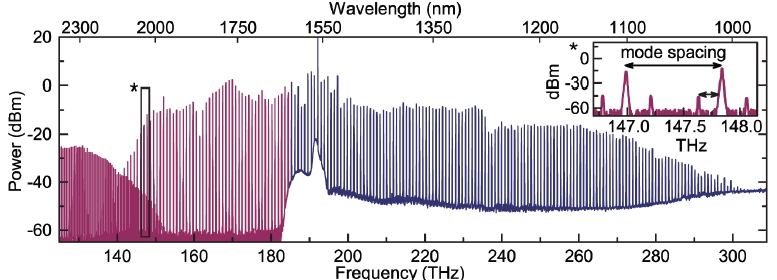
\includegraphics[]{octave_comb_mlg}
  %\caption{Спектр октавной гребенки, полученной из тороидального резонатора из плавленого кварца диаметром $40$ мкм. Расстояние между линиями гребенки $850$ ГГц. Взято из \cite{DelHaye2011}}
  %\label{octave_comb_mlg}
%\end{figure}


%В работе \cite{Herr2012} экспериментально изучалась динамика генерации гребенок в двух различных резонаторах: $MgF_2$ (ширина резонанса $1$ МГц), и $Si_3N_4$ (200 МГц). Геометрии резонаторов изображены на рис. \ref{mgf2_si3N4_resonators}.

%\begin{figure}
%  \centering
%  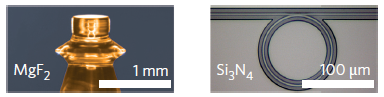
\includegraphics[]{mgf2_si3N4_resonators}
%  \caption{Форма резонаторов, в которых наблюдались оптические гребенки. Взято из \cite{Herr2012}}
%  \label{mgf2_si3N4_resonators}
%\end{figure}
%Для генерации первых боковых мод и далее всей гребенки лазер накачки постоянной мощности изначально сильно отстроен в синюю область от резонансной моды. Далее отстройка накачки медленно уменьшается, так что все больше и больше света связывается с резонансом. В некоторой точке достигается параметрический порог и возникает первая пара боковых мод. Экспериментальный вид спектра гребенок для обоих резонаторов представлен на рис. \ref{universal_formation_mlg}. Рассматриваются 2 сценария развития гребенки: а) первые образовавшиеся боковые моды являются соседними к моде накачки резонатора; б) первые боковые моды образуются вдалеке (по номеру моды) от накачки. Используется разложение собственных мод невозбужденного резонатора $\omega_\mu=\omega_0+D_1\mu+\frac{1}{2}D_2\mu^2$, где $D_1$ соответствует ОСД резонатора, $D_2$ - разность двух соседних ОСД около центральной частоты $\omega_0$. Далее аналитически решается система связанных уравнений для двух боковых мод и моды накачки. Собственные значения этой системы дают условие на порог генерации боковых мод. Откуда можно получить выражение для минимального номера первично возбуждаемых мод $\mu_{th,min}=\sqrt{\frac{\kappa}{D_2}}$, где $\kappa$ обозначает суммарные потери в резонаторе и элементе связи.
%\begin{figure}
%  \centering
%  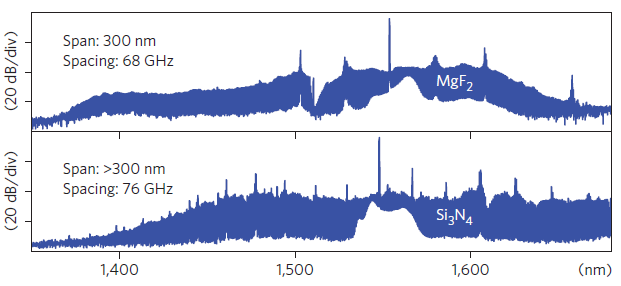
\includegraphics[]{universal_formation_mlg}
%  \caption{Спектр наблюдаемых гребенок. Мощность накачки для $MgF_2$ - $500$ мВт; для $Si_3N_4$ - $3$ Вт. Взято из \cite{Herr2012}}
%  \label{universal_formation_mlg}
%\end{figure}

%В работе \cite{Chembo2010pra} приводится общее описание сферических микрорезонаторов с модами типа шепчущей галереи (МШГ), дается вывод системы связанных уравнений (спектральное представление), описывающих динамику каждой моды. Аналитически выводится значение пороговой мощности, необходимой для начала генерации гребенки $P_{th}=\frac{n_0^2 V_0}{2\hbar\omega_0 n_2 c Q_0}$, где $n_0$ - показатель преломления, $V_0$ - эффективный объем моды, $\omega_0$ - частота накачки, $Q_0$ - собственная добротность резонатора, $n_2$ - нелинейная часть показателя преломления. В статье проведено численное моделирование этой системы для $200$ мод.

%Оптические гребенки наблюдались при разных геометриях резонаторов и разных типах связи с ними. В работе \cite{DelHaye2013} из цилиндрической заготовки из кварца при ее вращении выжигались $CO_2$ лазером резонаторы в форме микрокольца вокруг цилиндра диаметром от $170$ мкм до $8$ мм. В этих резонаторах удалось генерировать гребенку с расстоянием между модами от $300$ ГГц до $8.4$ ГГц соответственно. В работе \cite{Wang2013oe} использовался планарный кольцевой резонатор из нитрида кремния с использованием второго волновода для выходящего сигнала, при этом спектр на выходе был более гладким, т.к. спектральная линия большой мощности накачки не попадала в дроп-порт.

%Другой подход к моделированию оптических частотных гребенок основан не на системе связанных уравнений в спектральном представлении, а на решении уравнения Луджиато-Лефевера в пространственно-временном представлении. В работах \cite{Matsko2011} и \cite{Chembo2013} дан вывод этого уравнения из уравнений связанных мод. Решение уравнения Луджиато-Лефевера описывает в данном случае диссипативный временной солитон, распространяющийся в резонаторе. Экспериментальное наблюдение солитонов впервые было продемонстрировано в статье \cite{Herr2014}. Длительность солитона (полная ширина на половине высоты) составила около $200$ фс, период их следования около $28$ пс (для односолитонного режима). Экспериментальные данные первой демонстрации солитонов представлены на рис. \ref{experiment}

%\begin{figure}
%  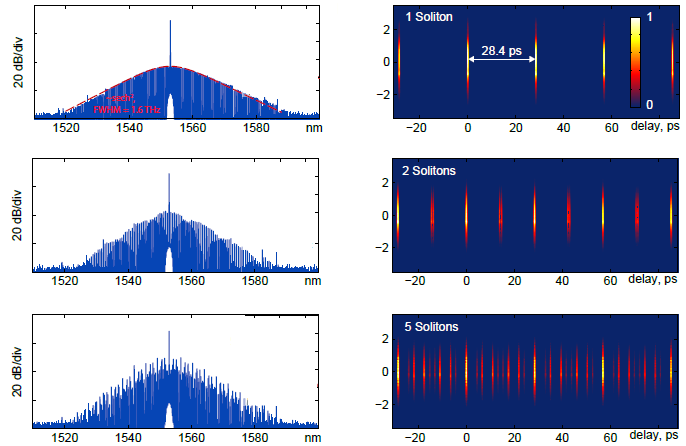
\includegraphics[]{experiment}
%  \caption{Экспериментально полученный спектр гребенки для одно-, двух и пяти солитонного режимов. Справа картина соответствующих импульсов во временном представлении. Взято из \cite{Herr2014}} \label{experiment}
%\end{figure}

%Обзор потенциальных применений оптических гребенок в микрорезонаторах дан в \cite{Kippenberg2011}. Используя компактные микрорезонаторы и один лазер накачки, можно сделать калибровку для астрономического спектрографа для видимого и ближнего ИК диапазонов, с межмодовым расстоянием $10-30$ ГГц. Такие устройства могут позволить измерить доплеровский сдвиг в спектре звезды с точностью, требуемой для обнаружения планет вне Солнечной системы. Ключевым преимуществом в этом случае является малый размер и масса системы.
           % Глава 1
\chapter{Численное моделирование} \label{chapt2}

\section{Теоретическое описание керровских гребенок в микрорезонаторах}

\subsection{Оптическая нелинейность в микрорезонаторах}
Поскольку оптические моды типа шепчущей галереи в резонаторах сочетают малый эффективный объем локализации поля с высокой добротностью, то порог проявления различных нелинейных эффектов оказывается низким \cite{Gorodetsky}. Одним из таких эффектов является нелинейный эффект четырехчастотного взаимодействия, приводящей к формированию оптической гребенки: два фотона переходят в боковые линии (рис. \ref{cascading}). Если накачка достаточно велика, то гребенка формируется благодаря каскадному процессу образования таких боковых линий, как суммы взаимодействий всевозможных 4 фотонов, удовлетворяющим частотным требованиям. Эффект возникает из-за материальной Керровской нелинейности среды.

\begin{figure}
  \centering
%  width=390pt,height=550pt
  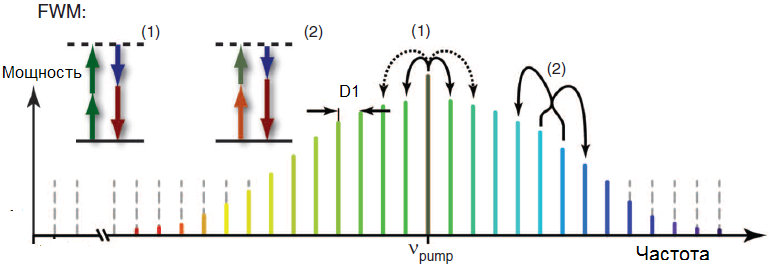
\includegraphics[]{FWM_Science}
  \caption{Эффект четырехчастотного взаимодействия. $(1)$ - вырожденный случай (два фотона одинаковой частоты переходят в фотоны большей и меньшей частоты), $(2)$ - невырожденный случай (все четыре фотона имеют разные частоты)} \label{cascading}
\end{figure}


Описание нелинейных оптических явлений можно проводить разложением вектора поляризации в ряд:
%
\begin{equation}
P(t)=\epsilon_0[\chi^{(1)}E(t)+\chi^{(2)}E^2(t)+\chi^{(3)}E^3(t)+\dots] =P^{(1)}(t)+P^{(2)}(t)+P^{(3)}(t)+\dots,
\end{equation}
%
где $\chi^{(1)}$ -- линейная восприимчивость, $\chi^{(2)},\chi^{(3)},\dots$ -- нелинейные восприимчивости второго, третьего порядков. $P^{(1)}(t),P^{(2)}(t),P^{(3)}(t)$ -- линейная и нелинейные поляризации второго и третьего порядков. Электрическая индукция в среде
%
\begin{equation}
D(t)=\epsilon E(t)=\epsilon_0E(t)+P,
\end{equation}
%
диэлектрическая проницаемость и показатель преломления $n=\sqrt{\epsilon}$ оказываются зависимыми от напряженности поля:
%
\begin{equation}
\epsilon=1+\chi^{(1)}+\chi^{(2)}E(t)+\chi^{(3)}E^2(t)+\dots,
\end{equation}
\begin{equation}
n=n_0+\frac{1}{2n_0}\chi^{(2)}E(t)+\frac{1}{2n_0}\chi^{(3)}E^2(t)+\dots
\end{equation}
%
В общем случае все коэффициенты являются тензорами, связывающими компоненты вектора поляризации со всеми возможными произведениями компонентов вектора \textbf{E}. В кристаллах, обладающих центром симметрии, а также в изотропных веществах из соображений симметрии $\chi^{(2)}=0$ и основной вклад вносит кубическая нелинейность, при которой изменение показателя преломления вещества пропорционально квадрату напряженности электрического поля. Она может быть обусловлена различными механизмами: ориентационным, электронным, стрикционным -- вместе они называются Керровской нелинейностью. Эффект четырехволнового взаимодействия относится к типу эффектов, в которых наведенная поляризация не колеблется с частотой падающего поля \cite{Gorodetsky}.

\subsection{Отдельная мода}
Рассмотрим действие оптической кубической нелинейности на отдельную высокодобротную моду микрорезонатора. Динамические уравнения для амплитуды поля моды можно получить исходя из уравнений электродинамики:
\begin{equation}\label{initial_electrod}
\nabla\times\nabla\times\textbf{E}+\mu_0\frac{\partial^2\textbf{D}}{\partial t^2}=0,
\end{equation}
\begin{equation}\label{D_induction}
\textbf{D}=\epsilon_0\textbf{E}+\textbf{P}.
\end{equation}
Подставим \eqref{D_induction} в \eqref{initial_electrod} получим волновое уравнение в среде в общей форме:
\begin{equation}
\nabla\times\nabla\times\textbf{E}+\frac{1}{c^2}\frac{\partial^2\textbf{E}}{\partial t^2}=-\frac{1}{\epsilon_0c^2}\frac{\partial^2\textbf{P}}{\partial t^2},
\end{equation}
где член в правой части, играющий роль возбуждающей силы позволяет учесть накачку, нелинейность и дисперсию в среде.
Слагаемое
\begin{equation}
\nabla\times\nabla\times\textbf{E}=\nabla(\nabla\cdot \textbf{E})-\nabla^2E,
\end{equation}
в нелинейном случае нельзя свести к одному векторному оператору Лапласа, т.к. $\nabla\cdot\textbf{E}\neq0$ из-за нелинейной связи векторов $\textbf{D}$ и $\textbf{E}$. Но мы все же пренебрегаем этим членом ввиду его малости. Выделим из поляризации линейную часть, тогда волновое уравнение можно записать в виде:
\begin{equation}\label{wave_eq_polarization}
\nabla\times\nabla\times\textbf{E}+\frac{n^2(\omega)}{c^2}\frac{\partial^2\textbf{E}}{\partial t^2} =-\frac{1}{\epsilon_0c^2}\frac{\partial^2\textbf{P}_{NL}}{\partial t^2}-\frac{1}{\epsilon_0c^2}\frac{\partial^2\textbf{P}_{p}}{\partial t^2},
\end{equation}
где $\textbf{P}_{NL}=\epsilon_0\chi^3(\omega=\omega+\omega-\omega)|\textbf{E}|^2\textbf{E}$, а $\textbf{P}_p$ описывает поляризацию, вызванную полем накачки.
Пусть невозбужденное поле некоторой моды (с номером $\mu$) в линейном случае описывается уравнением
\begin{equation}\label{Helmholz}
\nabla\times\nabla\times\textbf{$e_\mu$}-\frac{n^2(\omega)\omega^2}{c^2}\textbf{$e_\mu$}=0,
\end{equation}
и $e_\mu$ нормировано на максимум так, что $max(e_\mu)=1$, $\int|e_\mu|^2dV=V_{eff}$. Представим поле моды в виде:
\begin{equation}
\textbf{E}=\frac{1}{2}[a(t)\textbf{$e_\mu$}(\textbf{r})e^{-i\omega_pt}+\text{к.с.}],
\end{equation}
где $\omega_p$ -- частота гармонической накачки, близкая к собственной частоте $\omega_\mu$.

Подставляя в \eqref{wave_eq_polarization}, домножая его на $e_\mu^*$ и интегрируя по всему объему, получаем, отбрасывая члены второго порядка малости \cite{Gorodetsky}:
\begin{equation}
\frac{\partial a}{\partial t}+[-i\Delta\omega-i\eta|a|^2+\frac{\kappa_0}{2}+\frac{\kappa_c}{2}]a=iF,
\end{equation}
\begin{equation}
\eta=\frac{3\omega_\mu\chi^{(3)}}{8n^2}\frac{V_{eff}}{V_{jj}},
\end{equation}
\begin{equation}
V_{jj}=\frac{(\int_V|e_\mu|^2dV)^2}{\int_V|e_\mu|^4dV}.
\end{equation}
Здесь $\Delta\omega=\omega_p-\omega_\mu$ и формально добавлены собственные потери $\kappa_o=\kappa_a+\kappa_s=\frac{\omega_0}{\frac{1}{Q_0}+\frac{1}{Q_c}}$, включающие потери поглощения $\kappa_a$ и рассеяния $\kappa_s$, которые можно получить, вводя мнимую часть диэлектрической проницаемости, и потери в элемент связи $\kappa_c$ ($Q_0$ - собственная, $Q_c$ - нагруженная добротности резонатора), а $F$ -- обобщенная сила, учитывающая эффективность связи и мощность, попадающую через элемент связи $P_{in}$
\begin{equation}
F=\sqrt{\frac{2P_{\text{in}}\kappa_c}{\epsilon_0\epsilon V_{\text{eff}}}}
\end{equation}
Для мод шепчущей галереи \cite{Gorodetsky} $V_{jj}\simeq 2V_{eff}$.

\subsection{Несколько мод. Система связанных уравнений}
Рассмотрим процесс генерации гребенки, когда лазер накачки с постоянной мощностью изначально отстроен в область более высоких частот от резонансной частоты. Далее отстройка постепенно уменьшается, в некоторый момент достигается граница параметрической генерации и образуется первая пара боковых мод гребенки.

Пусть $\omega_p$ -- частота накачки лазером, $A_\mu$ амплитуды мод, нормированные, т.ч. $|A_\mu|^2$ число квантов в моде $\mu$. Все номера мод определены относительно моды накачки $\mu=0$. Выражение для собственных мод резонатора с частотами с точностью до кубического члена дисперсии \cite{Herr2012}:
\begin{equation}\label{dispersion_eq}
\omega_\mu=\omega_0+D_1\mu+\frac{1}{2}D_2\mu^2+\frac{1}{6}D_3\mu^3,
\end{equation}
где $D_1$ - область свободной дисперсии (ОСД) резонатора, $D_2$ - разница между двумя соседними ОСД на центральной частоте $\omega_0$. Представим теперь решение в виде:
\begin{equation}\label{SMA_E}
E(r,t)=\sum_\mu\frac{1}{2}A_\mu(t)e^{i\omega_\mu t}e_\mu(r)+\frac{1}{2}A_{ext}e^{i\omega_pt}e_0+\text{к.с.}
\end{equation}
где $\mu$ -- номер рассматриваемой моды, определенный набором ортонормированных собственных мод $e_\mu$ с частотой $\omega_\mu$ и амплитудой $A_\mu(t)$. Нормировка здесь выбрана так, чтобы $|A_\mu|^2$ соответствовало числу фотонов в моде. Направление накачки $A_{ext}$ определяется единичным вектором $e_0$. Пространственные и временные части поля разделяются, мода имеет одинаковую амплитуду по всему пространству. Амплитуда моды меняется медленно $|\dot{A}_\mu(t)|\ll2\omega_\mu|A_\mu(t)|$. Внешняя накачка $\omega_p$ близка к резонансной частоте системы. Пренебрегаем зависимостью $n_\mu(\omega)$ и другими типами взаимодействий мод, кроме четырехчастотного. Рассмотрим левую часть \eqref{wave_eq_polarization}, учитывая \eqref{Helmholz}:
%
\begin{equation}
\frac{1}{2}\sum_\mu(\nabla^2A_\mu e^{i\omega_\mu t}e_\mu+\text{к.с.})-\frac{1}{2c^2}\sum_\mu(\ddot{A_\mu}e_\mu e^{i\omega_\mu t}+(i\omega_\mu)^2e^{i\omega_\mu t}A_\mu e_\mu+\text{к.с.})=\sum_\mu i\omega_\mu n^2 \dot{A_\mu}e^{i\omega_\mu t}e_\mu+\text{к.с.}
\end{equation}
%
Домножим на $\frac{1}{2}(e_\mu+e_\mu^*)$ и проинтегрируем по всему пространству, учитывая ортогональность мод:

\begin{equation}
\int(\sum_\mu i\omega_\mu n^2 \dot{A_\mu}e^{i\omega_\mu t}e_\mu+\text{к.с.})e_\mu dV=\frac{i\hbar\omega_\mu^2}{2\epsilon_0n^2}\dot{A_\mu}e^{i\omega_\mu t}+\text{к.с.}
\end{equation}

Для правой части \eqref{wave_eq_polarization} после возведения в куб и домножения на $\frac{1}{2}(e_\mu+e_\mu^*)$ оставляем члены вида $e_\alpha e_\beta e_\gamma^* e_\mu^* e^{i(\omega_\alpha+\omega_\beta-\omega_\gamma-\omega_\mu)t}$

Окончательно можно получить выражения, определяющие динамику амплитуд \cite{Herr2012}\cite{Chembo2010pra}.
\begin{equation}\label{set_am}
\frac{\partial A_\mu}{\partial t}=-\frac{k}{2}A_\mu+\delta_{\mu 0}\sqrt{k_{ext}}se^{-i(\omega_p-\omega_0)t}+ig\sum_{\mu^\prime,\mu^{\prime\prime},\mu^{\prime\prime\prime}} \Lambda D A_{\mu^\prime}A_{\mu^{\prime\prime}}A_{\mu^{\prime\prime\prime}}^*e^{-i(\omega_{\mu^\prime}+\omega_{\mu^{\prime\prime}}-\omega_{\mu^{\prime\prime\prime}}-\omega_\mu)t},
\end{equation}
где $\kappa=\kappa_0+\kappa_{ext}$ - формально добавленные потери в резонаторе как сумма внутренних потерь $\kappa_0$ и связи с волокном $\kappa_{ext}$. Начальная фаза накачки $0$, $s=\sqrt{P_{in}/\hbar\omega_0}$ описывает амплитуду накачки $P_{in}$, $\delta_{\mu0}$ -- символ Кронекера. $D=2$ при $\mu^\prime\neq\mu^{\prime\prime}$, в других случаях $D=1$.
\begin{equation}
\Lambda=\frac{\int e_{\mu^\prime}e_{\mu^{\prime\prime}}e_{\mu^{\prime\prime\prime}}^*e_\mu^*dV}{\int|e_\mu|^4dV}
\end{equation}

Коэффициент нелинейной связи:
\begin{equation}
g=\frac{\hbar\omega_0^2cn_2}{n_0^2V_{eff}}
\end{equation}
описывает кубическую нелинейность среды с показателем преломления $n_0$, нелинейной частью показателя преломления $n_2$, эффективным нелинейным объемом резонатора $V_{eff}$. Физически $g$ показывает сдвиг частоты каждого фотона из-за керровской нелинейности среды. Для четырехчастотного взаимодействия $\hbar\omega+\hbar\omega^\prime\rightarrow\hbar\omega^{\prime\prime}+\hbar\omega^{\prime\prime\prime}$. Это условие всегда выполняется для эквидистантных мод, однако для мод шепчущей галереи (МШГ) четырехчастотное взаимодействие возможно при $|\omega+\omega^\prime-\omega^{\prime\prime}-\omega^{\prime\prime\prime}|\ll\Delta\omega\mu$. Поэтому суммирование проводится по всем индексам, удовлетворяющим $\mu=\mu^\prime+\mu^{\prime\prime}-\mu^{\prime\prime\prime}$.

В \cite{Matsko2005} показывается, что уравнение \eqref{set_am} можно получить, решая задачу с нелинейным Гамильтонианом.

Систему \eqref{set_am} можно переписать, убрав явную временную зависимость в правой части, и перенормировать все переменные и коэффициенты в единицах ширины резонансов $\kappa/2$, сделав их безразмерными \cite{Herr2012}. Получим:
\begin{equation}
f=\sqrt{\frac{8\eta g}{\kappa^2s}},
\end{equation}
\begin{equation}
d_2=\frac{D_2}{\kappa},
\end{equation}
\begin{equation}
\zeta_\mu=\frac{2(\omega_\mu-\omega_p-\mu D_1)}{\kappa}=\zeta_0+d_2\mu^2,
\end{equation}
\begin{equation}
\tau=\frac{\kappa t}{2},
\end{equation}
\begin{equation}\label{normirovka}
a_\mu=A_\mu\sqrt{\frac{2g}{k}}e^{-i(\omega_\mu-\omega_p-\mu D_1)t},
\end{equation}
\begin{equation}
\eta=\frac{k_{ext}}{k}=\frac{1}{2}.
\end{equation}
Окончательно получим систему уравнений для численного моделирования:

\fbox{
\begin{minipage}{6in}
\begin{equation}\label{compute_eq}
\frac{\partial a_\mu}{\partial \tau}=-[1+i\zeta_{\mu}]a_\mu+i\sum_{\mu^\prime\le\mu^{\prime\prime}} (2-\delta_{\mu^\prime\mu^{\prime\prime}})a_{\mu^\prime}a_{\mu^{\prime\prime}}a_{\mu^\prime+\mu^{\prime\prime}-\mu}^*+\delta_{0\mu}f.
\end{equation}
\end{minipage}}

\subsection{Уравнение Луджиато-Лефевера}

Задачу можно рассматривать в пространственно-временном представлении. Система в этом виде описывается уравнением Луджиато-Лефевера (LLE) \cite{Lugiato1987}. Это уравнение получается из нелинейного уравнения Шредингера (НУШ) добавлением слагаемых, отвечающих за диссипацию и накачку. Можно сказать, что оно же является частным случаем комплексного уравнения Гинзбурга-Ландау \cite{Akhmediev2005}. НУШ описывает распространение коротких световых импульсов в нелинейной среде с дисперсией \cite{Boyd2008}. НУШ является интегрируемой системой, для поиска решений которой используется метод обратной задачи рассеяния \cite{Akhmediev2003}. Уравнение Луджиато-Лефевера не является интегрируемой системой. Вывод уравнения LLE дан в \cite{Matsko2011},\cite{Chembo2013}.

Рассмотрим медленно меняющуюся амплитуду суммарного поля:
\begin{equation}\label{total_field}
A(\phi,t)=\sum_\mu A_\mu(t)e^{i(\omega_\mu-\omega_0)t-i(\mu-\mu_0)\phi},
\end{equation}
где $\phi=[-\pi,\pi]$ азимутальный угол. Частные производные:

\begin{equation}\label{partial_t}
\frac{\partial A}{\partial t}=\sum_\mu(\dot{A_\mu}+i(\omega_\mu-\omega_0)A_\mu)e^{i(\omega_\mu-\omega_0)t-i(\mu-\mu_0)\phi},
\end{equation}
\begin{equation}\label{partial_phi}
i^n\frac{\partial^n A}{\partial \phi^n}=\sum_\mu(\mu-\mu_0)^n A_\mu e^{i(\omega_\mu-\omega_0)t-i(\mu-\mu_0)\phi}.
\end{equation}

Ограничиваясь вырожденным случаем $D=1$ подставим \eqref{total_field}-\eqref{partial_phi} в \eqref{set_am}. Производя замену $d_2=D_2/\kappa$, $\theta=\phi\sqrt{\frac{1}{2d_2}}$, $\tau=\kappa t/2$, $\psi(\tau,\theta)=\sum a_\mu(\tau)e^{i\mu\theta}$ получим:

\fbox{
\begin{minipage}{6in}
\begin{equation}\label{LLE}
i\frac{\partial \psi}{\partial \tau}+\frac{1}{2}\frac{\partial^2 \psi}{\partial \theta^2}+|\psi|^2\psi=(-i+\zeta_0)\psi+if,
\end{equation}
\end{minipage}}

где $\zeta_0, f$ совпадают с \eqref{compute_eq}. Для уравнения LLE не известны точные аналитические решения. Для численного решения существует несколько способов. Так, для стационарного случая \cite{Akhmediev2005} $\frac{\partial \psi}{\partial \tau}=0$ делается Фурье преобразование, полученная система алгебраических уравнений решается методом Ньютона. Другим используемым методом является Фурье метод расщепления по параметрам (Split Step Fourier Method - SSFM).

\section{Численные методы исследования}

\subsection{Метод Рунге-Кутты}
Уравнения для моделирования \eqref{compute_eq} представляет собой систему обыкновенных дифференциальных уравнений первого порядка. Для численного решения обыкновенных дифференциальных уравнений существуют метод Рунге-Кутты, экстраполяционный метод Ричардсона, метод предиктор-корректор и др \cite{Press2002}.

Метод предиктор-корректор хорошо работает для гладких функций. В нем сохраняются все предыдущие рассчитанные значения функции и используются для оценки значения на следующем шаге. В методе Ричардсона используются экстраполяция рассчитанного значения функции к другому значению, которое получилось бы, если бы шаг сетки был меньше текущего. Эти методы сложнее в реализации и требуют большей вычислительной мощности.

В работе использовался широко известный метод Рунге-Кутты. Рассмотрим систему:
%
\begin{equation}
\frac{dy_i(x)}{dx}=f_i(x,y_1,\dots,y_N),\quad i=1,\dots,N,
\end{equation}
%
где функции $f_i$ известны. Заданы начальные условия $y_i(x_s)$, требуется найти $y_i(x_f)$ в конечной точке или во всех точках сетки.

Наиболее часто используется метод Рунге-Кутты 4 порядка (4ый порядок точности). Используется фиксированный шаг $h$ по $x$. Для проверки точности работы алгоритма можно сравнивать результаты, полученные при величинах шага $h$ и $\frac{h}{2}$. Такое сравнение требует значительного вычислительного времени, поэтому лучше ввести адаптивный контроль за работой алгоритма, изменять размер шага во время счета и следить за полученной ошибкой. Фелберг \cite{Press2002} предложил метод пятого порядка с 6 вычислениями функции, т.ч. другая комбинация этих функций дает метод четвертого порядка точности. Разница между двумя вычисленными $y(x+h)$ используется для оценки ошибки и корректировки шага. Общий вид формул метода Рунге-Кутты пятого порядка:
\begin{equation}
k_1=hf(x_n,y_n),
\end{equation}
\begin{equation}
\begin{split}
k_2=hf(x_n+a_2h,y_n+b_{21}k_1),\\
\dots
\end{split}
\end{equation}
\begin{equation}
k_6=hf(x_n+a_6h,y_n+b_{61}k_1+\dots+b_{65}k_5),
\end{equation}
\begin{equation}
y_{n+1}=y_n+c_1k_1+c_2k_2+c_3k_3+c_4k_4+c_5k_5+c_6k_6+O(h^6).
\end{equation}
Формула для четвертого порядка:
\begin{equation}
y_{n+1}^*=y_n+c_1^*k_1+c_2^*k_2+c_3^*k_3+c_4^*k_4+c_5^*k_5+c_6^*k_6+O(h^5).
\end{equation}
Ошибка выражается как:
\begin{equation}
\Delta\equiv y_{n+1}-y_{n+1}^*=\sum_{i=1}^6(c_i-c_i^*)k_i.
\end{equation}
Значения коэффициентов, полученных Cash-Karp \ref{Cash_Karp}, \cite{Press2002}:

\begin{table} [htbp]% Пример записи таблицы с номером, но без отображаемого наименования
	\centering
	\parbox{15cm}{% чтобы лучше смотрелось, подбирается самостоятельно
        %\captionsetup{format=tablenocaption}% должен стоять до самого caption
        \caption{Cash-Karp коэффициенты}%
        \label{Cash_Karp}%

\begin{tabular}{||c|c|c|c|c|c|c|c|c||}
%\hline
%\multline{Cash-Karp коэффициенты}
\hline
i & $a_i$ & & & $b_{ij}$ & & & $c_i$ & $c_i^*$\\
\hline
$1$ & & & & & & & $\frac{37}{378}$ & $\frac{2825}{27648}$\\
\hline
$2$ & $\frac{1}{5}$ & $\frac{1}{5}$ & & & & & $0$ & $0$\\
\hline
$3$ & $\frac{3}{10}$ & $\frac{3}{40}$ & $\frac{9}{40}$ & & & & $\frac{250}{621}$ & $\frac{18575}{48384}$\\
\hline
$4$ & $\frac{3}{5}$ & $\frac{3}{10}$ & $-\frac{9}{10}$ & $\frac{6}{5}$ & & & $\frac{125}{594}$ & $\frac{13525}{55296}$\\
\hline
$5$ & 1 & $-\frac{11}{54}$ & $\frac{5}{2}$ & $-\frac{70}{27}$ & $\frac{35}{27}$ & & $0$ & $\frac{277}{14336}$\\
\hline
$6$ & $\frac{7}{8}$ & $\frac{1631}{55296}$ & $\frac{175}{512}$ & $\frac{575}{13824}$ & $\frac{44275}{110592}$ & $\frac{253}{4096}$ & $\frac{512}{1771}$ & $\frac{1}{4}$\\
\hline
& $j=$ & 1 & 2 & 3 & 4 & 5 & & \\
\hline
\end{tabular}
}
\end{table}

Введем требуемую точность $\Delta_0$, если при шаге $h_1$ получилась ошибка $\Delta_1$, то  \cite{Press2002}:
\begin{equation}\label{h_steps}
h_o=h_1\left|\frac{\Delta_0}{\Delta_1}\right|^{0.2}.
\end{equation}
Если $\Delta_1 > \Delta_0$, то \eqref{h_steps} показывает насколько нужно уменьшить шаг и повторить расчет текущего шага. Если $\Delta_1 < \Delta_0$, то \eqref{h_steps} показывает насколько можно увеличить шаг для следующего вычисления. Поскольку $\Delta_0$ -- вектор требуемой точности, то сравнение можно проводить по отклонению каждого элемента.

%\begin{wrapfigure}{l}{0.7\linewidth}
%  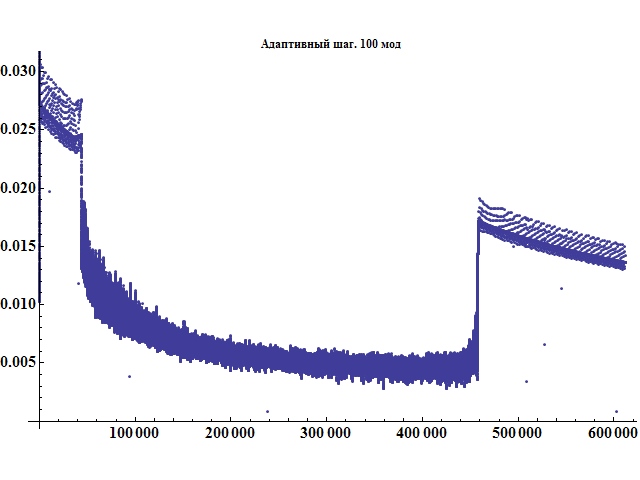
\includegraphics[scale = 0.5]{adaptive_step_100}
%\caption{Зависимость величины адаптивного шага от номера итерации} \label{adaptive}
%\end{wrapfigure}

В программе был добавлен параметр минимальный шаг, ниже которого адаптивное уменьшение запрещено - программа переходит к расчету на следующий узел времени. На практике в большинстве симуляций адаптивность работала на увеличение шага на гладких участках амплитудных кривых, и на уменьшение шага в областях хаотического режима. Количество повторных пересчетов с уменьшенным шагом в среднем составляло около $10\%$ от общего числа шагов по времени.
%Рис. \ref{adaptive} показывает величину шага от его номера.

Адекватность использования метода Рунге-Кутты была проверена хорошим совпадением результатов численного моделирования и эксперимента \cite{Herr2014}. Однако по результатам симуляции видно, что решение чувствительно к малым изменениям параметров. Области генерации могут отличаться даже при новом случайном затравочном шуме в каждой моде.

\subsection{Фурье метод расщепления по параметрам (SSFM)}
Для решения НУШ наиболее быстрым является Фурье метод расщепления по параметрам. Применим его к уравнению Луджиато-Лефевера:
\begin{equation}
i\frac{\partial \psi}{\partial t}+\frac{1}{2}\frac{\partial^2 \psi}{\partial \theta^2}+|\psi|^2\psi=(-i+\zeta_0)\psi+if.
\end{equation}
Выделим линейную $\hat{L}$ и нелинейную $\hat{N}$ части оператора:
\begin{equation}
\hat{N}=i|\psi|^2\psi+f,
\end{equation}
\begin{equation}
\hat{L}=\frac{i}{2}\frac{\partial^2\psi}{\partial \theta^2}-(i\zeta_0+1)\psi.
\end{equation}
Решение на следующем шаге по времени дается выражением:
\begin{equation}
\psi(\theta,t+\tau)\approx\exp (i\tau(\hat{L}+\hat{N}))\psi(\theta,t).
\end{equation}
Это выражение является точным, если $|\psi|^2=const$. Далее происходит разделение по времени:
\begin{equation}
\exp (i\tau(\hat{L}+\hat{N}))\psi(\theta,t)
\approx\exp(i\tau\hat{L})\times\exp(i\tau\hat{N})\psi(\theta,t).
\end{equation}
Это выражение является точным, если $\hat{L}$ и $\hat{N}$ коммутируют. Данную схему можно рассматривать как последовательное решение уравнения для нелинейного оператора \eqref{nonlinear_split_eq}, подстановку полученного значения в \eqref{linear_split_eq} начальным условием. Далее решается уравнение для линейного оператора, решение подставляется начальным условием обратно в \eqref{nonlinear_split_eq}, процедура повторяется.
\begin{equation}\label{nonlinear_split_eq}
\psi_t=\hat{N}\psi,
\end{equation}
\begin{equation}
\tilde{\psi}(\theta,t+\tau)=C\exp(i|\psi|^2\tau)-\frac{f}{i|\psi|^2},
\end{equation}
\begin{equation}\label{linear_split_eq}
\psi_t=\hat{L}\psi,
\end{equation}
\begin{equation}
\psi(\theta,t+\tau)=F.T^{-1}[\exp(-\tau(ik^2+i\zeta_0+1))F.T.[\tilde{\psi}(\theta,t+\tau)]].
\end{equation}

\subsection{Ускорение вычислений для системы связанных уравнений}
Пусть гребенка состоит из $2K+1$ мод, тогда количество нелинейных членов в сумме в \eqref{compute_eq} для всех уравнений равно:
\begin{equation}
\frac{1}{3}(K+1)(8K^2+7+3).
\end{equation}
Время счета для всех мод $T\varpropto K^3+O(K^2)$. Время счета однопоточной программы может быть значительным (больше суток) уже при $K=200$, поэтому возникла необходимость ускорить вычисления путем распараллеливания.

Существуют методы распараллеливания на CPU, использующие POSIX-треды операционной системы с моделью общей памяти (shared-memory). Другой способ - использовать протокол MPI (Message Passing Interface) и модель распределенной памяти (distributed memory). На вычислительном кластере МГУ возможен запуск программ, написанных на языке C или Fortran с использованием MPI библиотек.

Была написана программа на языке C с использованием стандарта MPI, которая реализует метод Рунге-Кутты с адаптивным шагом для уравнения \eqref{compute_eq}. В программе предусмотрена перестройка частоты накачки, рост амплитуды накачки во времени, все входящие в уравнение коэффициенты настраиваются. Результатом работы программы являются зависимости амплитуд мод от отстройки накачки (меняющейся во времени).

Сумма в правой части \eqref{compute_eq} $\sum_{\mu^\prime\le\mu^{\prime\prime}} (2-\delta_{\mu^\prime\mu^{\prime\prime}})a_{\mu^\prime}a_{\mu^{\prime\prime}}a_{\mu^\prime+\mu^{\prime\prime}-\mu}^*$ считается параллельно на нескольких CPU. Каждый из них считает суммы для определенный набора своих мод $\mu$. Корневой процесс (root) рассылает и получает массив амплитуд $a_i$ от других процессов. Далее root рассчитывает значение функции на следующем шаге методом Рунге-Кутта.

Программа была скомпилирована и запущена на ubuntu (реализация OpenMPI-1.6.3), Windows (реализация MPICH2 32bit и 64bit версии) и на суперкомпьютере Ломоносов (OpenMPI-1.5.5). На локальном компьютере быстрее всего работала 64 битная версия под Windows, хотя linux версия запускалась в виртуальной машине. На Ломоносове при равном количестве процессоров программа считает быстрее, чем на ноутбуке. Однако существуют ограничения для пользователя - время счета не более 3 суток, максимальное число процессоров около 100. При таких ограничениях не удалось провести симуляцию для 1000 мод.

На рис. \ref{bechmarking} представлена зависимость времени счета для $200$ мод от количества задействованных процессоров. Заметного улучшения производительности не наблюдается уже при 40 и более процессорах. Это можно объяснить тем, что суммы в нелинейных членах считаются для $200$ мод достаточно быстро, корневой процесс, считающий сам метод Рунге-Кутты, не успевает вычислять и рассылать значения массива мод на новом шаге по времени. Дочерние процессы в это время бездействуют.
%\begin{wrapfigure}{l}{0.7\linewidth}
%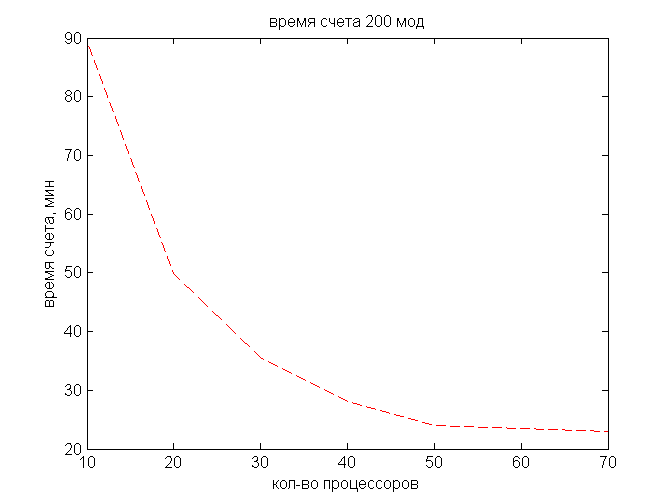
\includegraphics[scale = 0.6]{benchmarking}
%\caption{Ускорение счета} \label{bechmarking}
%\end{wrapfigure}

\begin{figure}
 \centering
 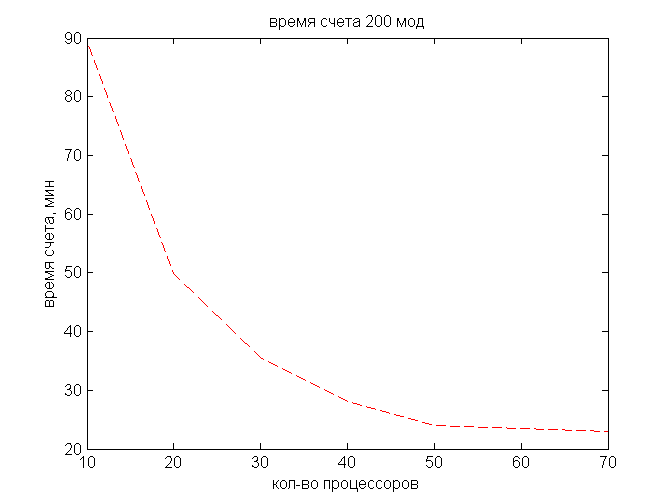
\includegraphics[scale = 0.8]{benchmarking}
 \caption{Ускорение счета} \label{bechmarking}
\end{figure}

В целом время счета нелинейно зависит от диапазона перестройки и сценария симуляции. Заранее оценить его для запуска на кластере проблематично.

Существенное сокращение времени счета было достигнуто методом, предложенным в статье \cite{Hansson2014oc}. Сумма в правой части \eqref{compute_eq} преобразуется с хорошей точностью к виду:
\begin{equation}\label{wabnitz_summation}
\sum_{\mu^\prime\le\mu^{\prime\prime}} (2-\delta_{\mu^\prime\mu^{\prime\prime}})a_{\mu^\prime}a_{\mu^{\prime\prime}}a_{\mu^\prime+\mu^{\prime\prime}-\mu}^*\approx F.T^{-1}[|f_j|^2f_j]
=\frac{1}{N}\sum_{j=0}^{N-1}(|f_j|^2f_j)e^{i2\pi j\mu /N},
\end{equation}
где прямое дискретное преобразование Фурье
\begin{equation}
f_j=F.T[a_\mu]=\sum_{j=0}^{N-1}a_\mu e^{-i2\pi j\mu/n}.
\end{equation}

Было проведено численное сравнение двух методов вычисления правой части. Для гладкого спектра, обращающегося в $0$ на концах, совпадение двух результатов хорошее. Для реального спектра, генерируемого в резонаторе, результат, полученный через Фурье преобразование, всегда больше, чем при прямом вычислении суммы. Для мод, близких к центральной моде накачки, относительная ошибка приблизительно постоянна и составляет до $25\%$. Результаты сравнения даны на рис. \ref{ft_vs_sum}.

\begin{figure}
% \centering
 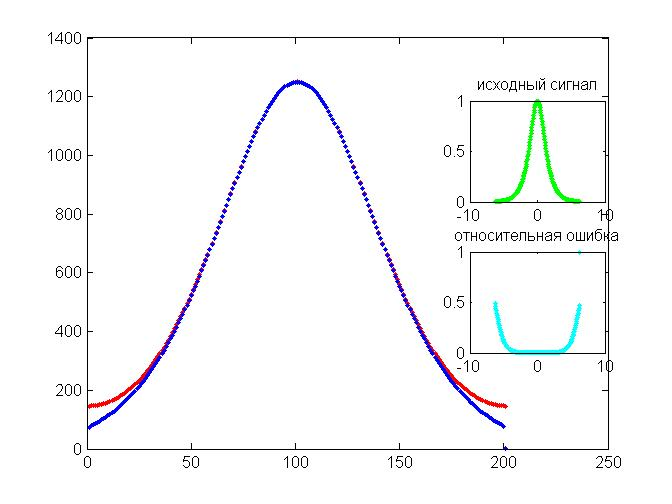
\includegraphics[width = 0.5\textwidth]{ft_vs_sum_sech}
 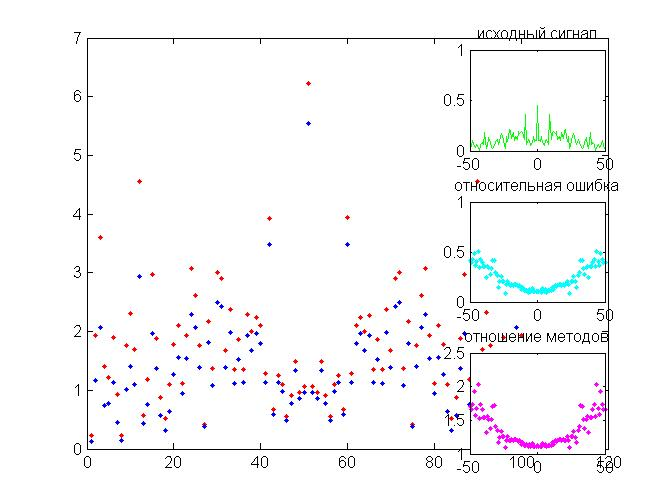
\includegraphics[width = 0.5\textwidth]{ft_vs_sum_comb1}
 \caption{Сравнение методов вычисления суммы. Синим обозначено прямое суммирование. Красным - с использованием \eqref{wabnitz_summation}. Исходный сигнал изображен на верхней вкладке ($sech(x)$ на левом рисунке и спектр реальной гребенки на правом)} \label{ft_vs_sum}
\end{figure}

Несмотря на выявленное отличие, конечные результаты симуляции гребенки двумя методами хорошо совпадают - одинаковы области генераций и наблюдаемые режимы. Тем самым затратное вычисление суммы заменяется на выполнение быстрого прямого и обратного Фурье преобразования. Предыдущая версия программы была переделана под расчет правой части уравнений с использованием стандартных FFT библиотек. Была реализована программа для NVIDIA GPU с использованием библиотеки CuFFT, однако она не дала заметных преимуществ по скорости счета и удобству последующей обработки данных, поэтому основное моделирование проводилось в среде MATLAB.

\section{Результаты моделирования}
\subsection{Используемые программы}
\begin{enumerate}
\item
Многопоточная программа под OpenMPI для симуляции связанных уравнений с суммой в правой части системы \eqref{compute_eq}. Скомпилированная (win32) программа доступна по \href{https://www.dropbox.com/sh/940djjdx3ojcsxy/_1JZsWTqPN/mpi}{ссылке}.
\item
Однопоточная программа для связанных уравнений с Фурье преобразованиями в правой части \eqref{wabnitz_summation}, использующая GPU для быстрого Фурье преобразования. Скомпилированная (win32) программа доступна по \href{https://www.dropbox.com/sh/940djjdx3ojcsxy/n4hBUtto1o/gpu}{ссылке}.
\item
MATLAB программа для связанных уравнений с Фурье преобразованиями в правой части \eqref{wabnitz_summation}.
\item
MATLAB программа для моделирования уравнения LLE \eqref{LLE} методом SSFM.
\item
Пакет Mathematica использовался для решения уравнения LLE \eqref{LLE} методом конечных разностей в функции NDSolve[ ].
\item Графический пользовательский интерфейс, написанный в MATLAB, объединяющий оба метода симуляции и позволяющий задавать параметры системы, сохранять промежуточные результаты на диск для последующей обработки и визуализации. Скриншот интерфейса представлен на рис. \ref{comb_gui}.
\end{enumerate}
\begin{figure}
 \centering
 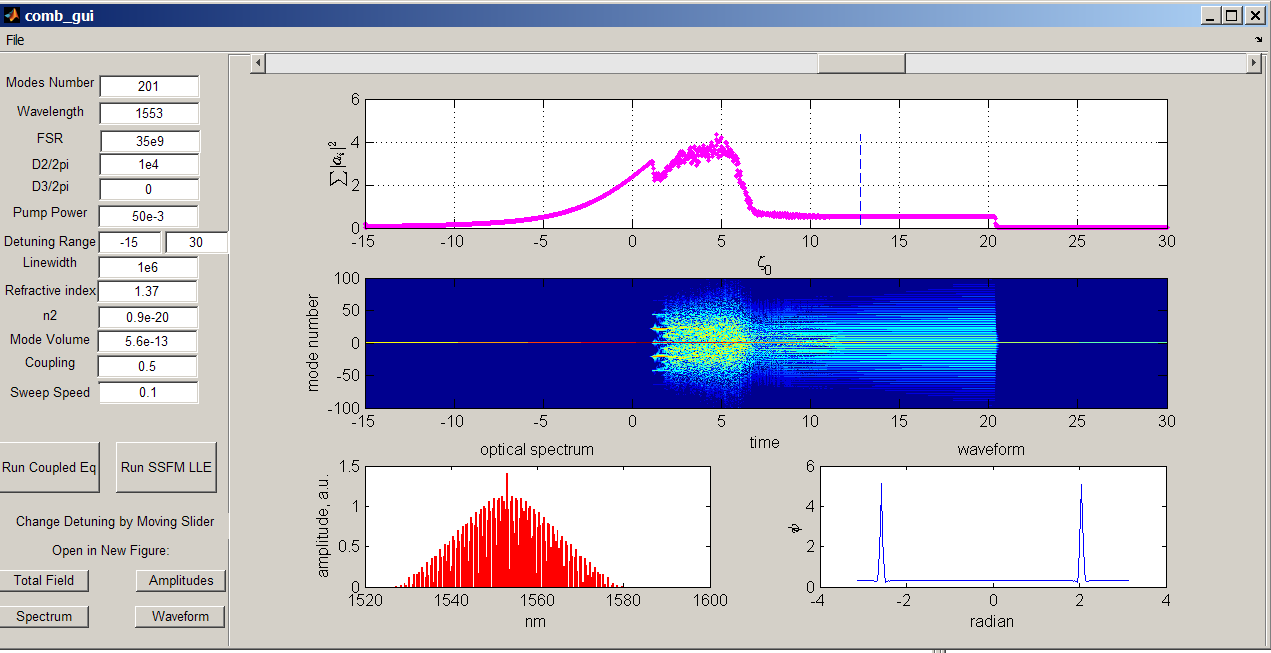
\includegraphics[scale=0.7]{comb_gui}
 \caption{Пользовательский интерфейс программы для численного моделирования CombGUI} \label{comb_gui}
\end{figure}

\subsection{Моделирование по экспериментальным данным}
\label{subsection_experiment}

Рассмотрим дисковый резонатор из $MgF_2$ с параметрами из статьи \cite{Herr2014}. Проверим адекватность теоретической модели путем сравнения результатов моделирования с экспериментальными наблюдениями (экспериментальные данные из \cite{Herr2014}). Начальным условием при решении системы связанных уравнений выступал затравочный шум в каждой моде, имеющий нормальное распределение, - приближение к квантовым нулевым флуктуациям в каждой моде. Используемые параметры:

\begin{equation}
Q_0=Q_c=5\times10^8,
\end{equation}
\begin{equation}
P_0=100\text{ мВт},
\end{equation}
\begin{equation}
\lambda_0=1.553\text{ мкм},
\end{equation}
\begin{equation}
\omega_0=1.213\times10^{15}\text{ Гц},
\end{equation}
\begin{equation}
n_0=1.376,
\end{equation}
\begin{equation}
V_{eff}=V_0=5.6\times10^{-13}\text{ м}^3,
\end{equation}
\begin{equation}
\kappa=\frac{\omega}{Q_0}=1.2\times10^6\text{ Гц},
\end{equation}
\begin{equation}
n_2=0.9\times10^{-20}\frac{\text{м}^2}{\text{Вт}},
\end{equation}
\begin{equation}
g=6.1\times10^{-4},
\end{equation}
\begin{equation}
D_1=2.21\times10^{11}\text{ Гц},
\end{equation}
\begin{equation}
D_2=6.28\times10^4\text{ Гц},
\end{equation}
\begin{equation}
D_3=-800\text{ Гц}.
\end{equation}

Результаты моделирования с помощью многопоточной программы представлены на рис. \ref{100modes},\ref{500modes},\ref{800modes} для $100$, $500$, $800$ мод соответственно.
\begin{figure}
%  \centering
%  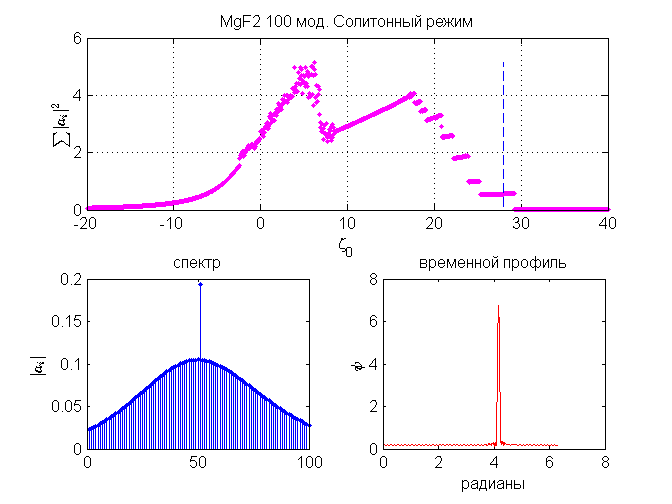
\includegraphics[width = 1\textwidth,height=0.5\textheight]{mgf2_100modes}
 % 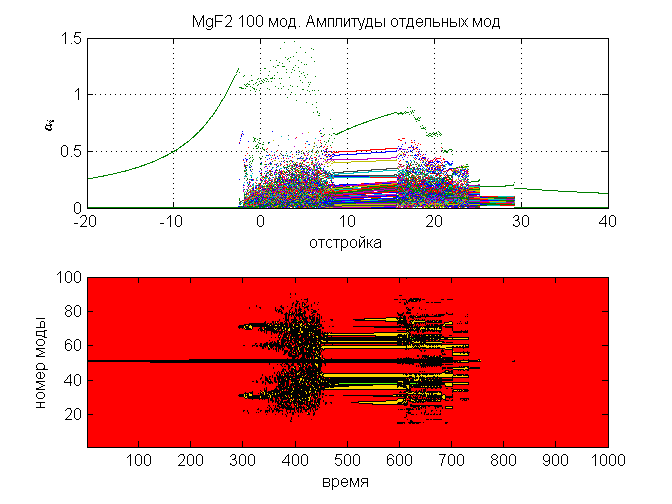
\includegraphics[width = 1\textwidth,height=0.5\textheight]{mgf2_100modes_modal}
  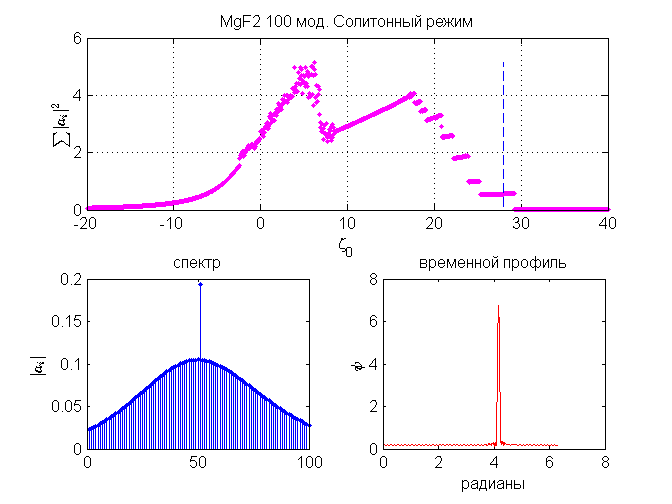
\includegraphics[width = 0.5\textwidth]{mgf2_100modes}
  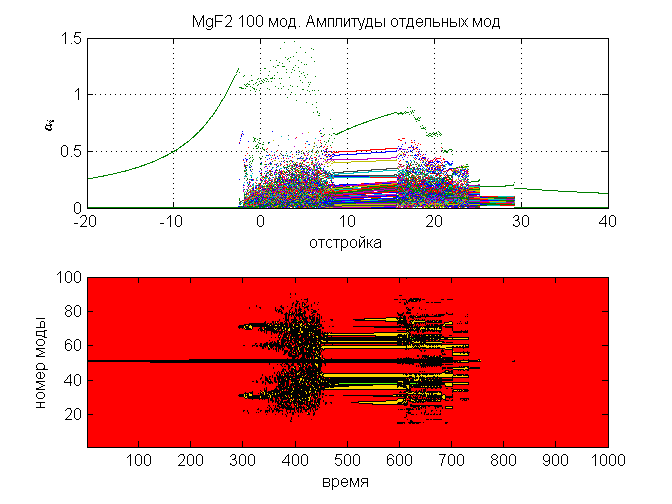
\includegraphics[width = 0.5\textwidth]{mgf2_100modes_modal}
  \caption{Моделирование 100 мод.Резонатор из $MgF_2$. Накачка $100$ мВт} \label{100modes}
\end{figure}

\begin{figure}
%  \centering
%  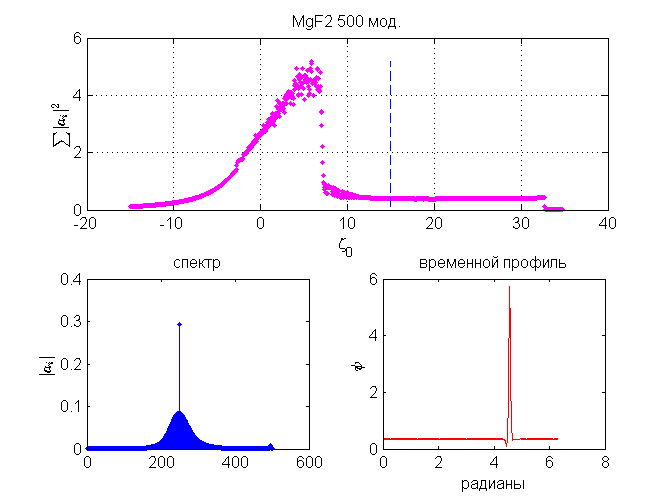
\includegraphics[width = 1\textwidth,height=0.5\textheight]{mgf2_500cluster}
 % 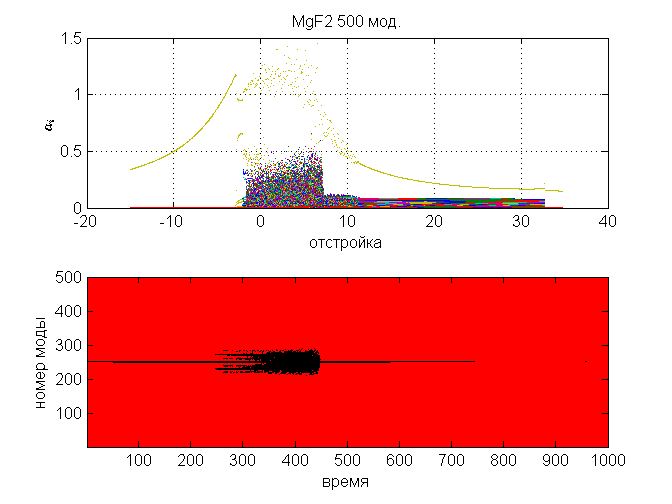
\includegraphics[width = 1\textwidth,height=0.5\textheight]{mgf2_500cluster_modal}
  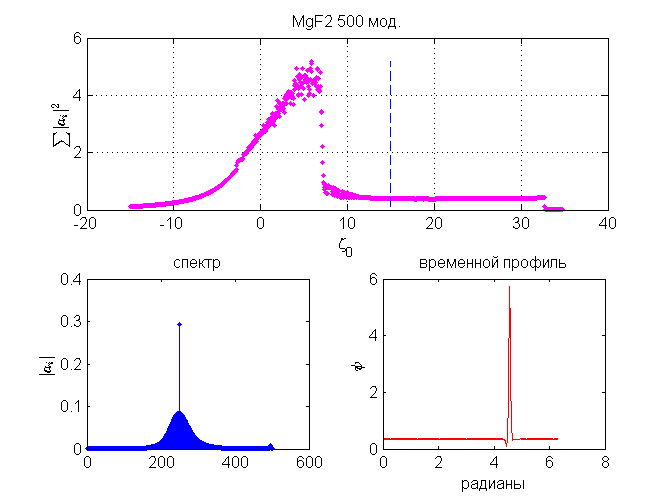
\includegraphics[width = 0.5\textwidth]{mgf2_500cluster}
  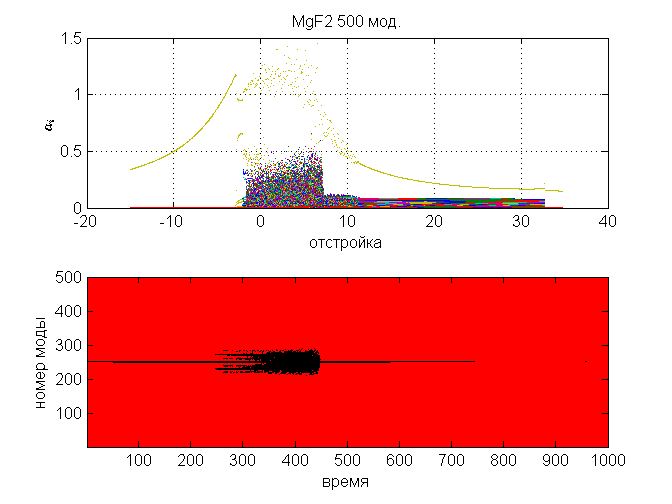
\includegraphics[width = 0.5\textwidth]{mgf2_500cluster_modal}
  \caption{Моделирование 500 мод.Резонатор из $MgF_2$. Накачка $100$ мВт} \label{500modes}
\end{figure}

\begin{figure}
%  \centering
%  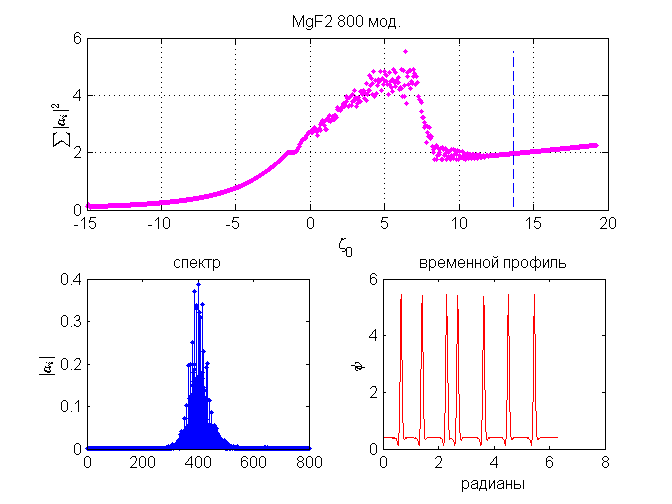
\includegraphics[width = 1\textwidth,height=0.5\textheight]{mgf2_800}
 % 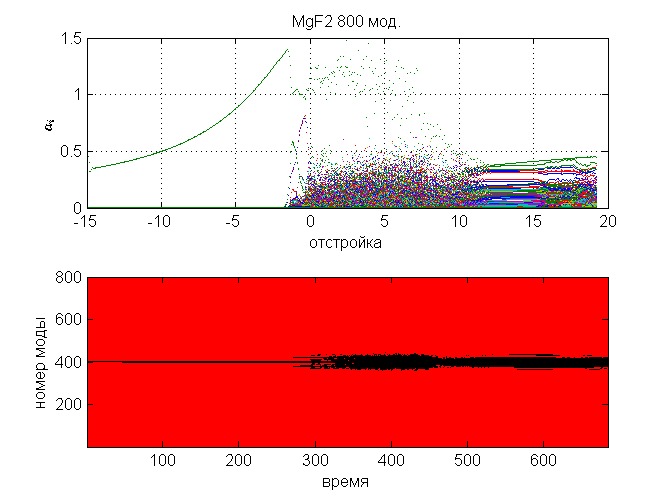
\includegraphics[width = 1\textwidth,height=0.5\textheight]{mgf2_800_modal}
  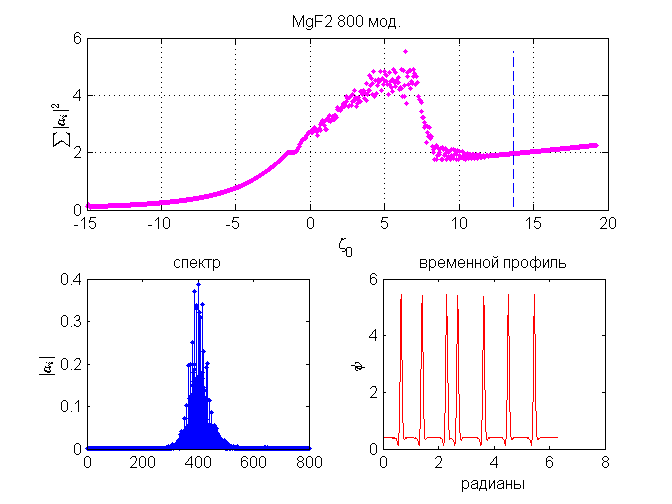
\includegraphics[width = 0.5\textwidth]{mgf2_800}
  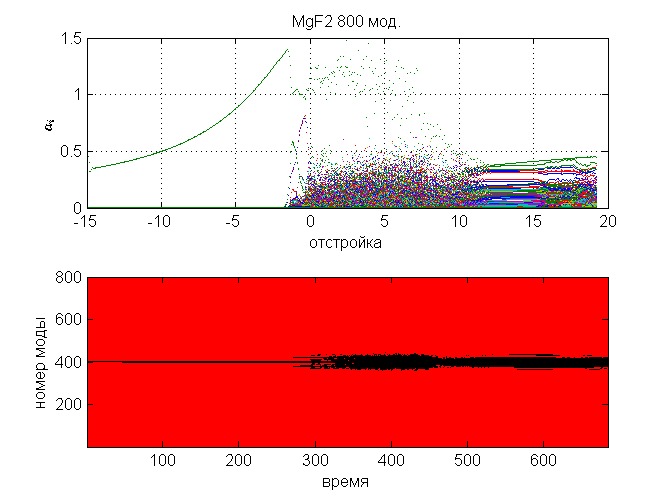
\includegraphics[width = 0.5\textwidth]{mgf2_800_modal}
  \caption{Моделирование 800 мод.Резонатор из $MgF_2$.Накачка $100$ мВт} \label{800modes}
\end{figure}

Число ОСД между соседними модами равно $1$. На левом верхнем графике представлена зависимость суммы квадратов амплитуд всех мод от величины отстройки лазера накачки. Отстройка изменяется линейно от начала до конца диапазона. Ось абсцисс поэтому соответствует временной шкале.  По оси ординат размерность дается нормировкой \eqref{normirovka}, по оси абсцисс отстройка частоты выражена в единицах, т.ч. $1$ соответствует перестройке на $1$ ширину резонансной кривой. Для наглядности приведены аналогичные графики амплитуд отдельных мод, и график, по которому можно понять какие номера мод были возбуждены в данный момент (правый рисунок). Синим цветом дан график спектра - зависимость модуля амплитуды от номера моды при данной отстройке. Текущая отстройка обозначена вертикальным пунктиром на верхнем графике. Красным показан пространственно-временной профиль $\psi(\tau,\Phi)=\sum a_\mu(\tau)e^{i\mu\Phi}$ при той же отстройке.

На всех трех графиках ($100$, $500$, $800$ мод) наблюдается сначала генерация только моды накачки, потом неустойчивая генерация гребенки, носящая хаотический характер. Далее при изменении отстройки возникают чередующиеся области стабильной и нестабильной генерации. В областях стабильной генерации возникают N импульсов (в зависимости от числа рассматриваемых мод), в следующей области N-1 и так далее. Наиболее интересна область генерации одного импульса (солитона), распространяющегося по экватору резонатора. Эта область наблюдалась экспериментально \cite{Herr2014}. Видны отличия между симуляциями $100$, $500$, $800$ мод: из хаотического режима гребенка переходит в устойчивые режимы с разным числом импульсов ($8$, $1$, $7$ соответственно), это связано с различными начальными условиям, затравочными шумаим. Также видно, что моды с номерами, удаленными от центральной моды накачки более, чем на $100$, не возбуждаются (или возбуждаются крайне слабо), что говорит о зависимости ширины гребенки от величины дисперсии второго порядка \cite{Brasch2016}. При большой по модулю аномальной дисперсии генерация широкой гребенки невозможна.

В целом результаты моделирования хорошо соответствуют эксперименту: ступенчатый вид зависимости суммы квадратов амплитуд всех мод от величины отстройки лазера накачки непосредственно наблюдался.

Рис. \ref{caf2} дает результат моделирования эксперимента из статьи \cite{Savchenkov2011}, в котором использовался сфероидальный резонатор из $CaF_2$ с параметрами:
$
Q_0=Q_c=3\times10^9,\quad
P_0=2\text{ мВт},\quad
\lambda_0=0.794\text{ мкм}, \quad
n_0=1.43,\quad
V_0=5.6\times10^{-15}\text{ м}^3,\quad
n_2=3.1\times10^{-20}\frac{\text{м}^2}{\text{Вт}},\quad
D_2=2.1\times10^4\text{ Гц},\quad
D_3=0\text{ Гц}.$

Резонатор был изготовлен методом механической полировки, подбирая размеры осей сфероида, можно задавать геометрическую дисперсию резонатора и тем самым регулировать центральную частоту гребенки.

По результатам численного моделирования (многопоточная программа) наблюдается генерация гребенки в более широком диапазоне перестройки лазера, чем для резонатора из $MgF_2$. Отчетливо видны области генерации солитонов. На графике амплитуд отдельных мод видно, что в областях генерации солитонов отдельные моды могут и не иметь гладких зависимостей. Полученный результат согласуется с выводами авторов статьи только в части наблюдения устойчивой гребенки. Экспериментально вид спектра ассиметричен, авторы объясняют это тем, что элемент связи находился около экватора резонатора и с большей эффективностью считывал сигнал от мод с меньшим номером и, соответственно, с меньшей частотой.

\begin{figure}
%  \centering
%  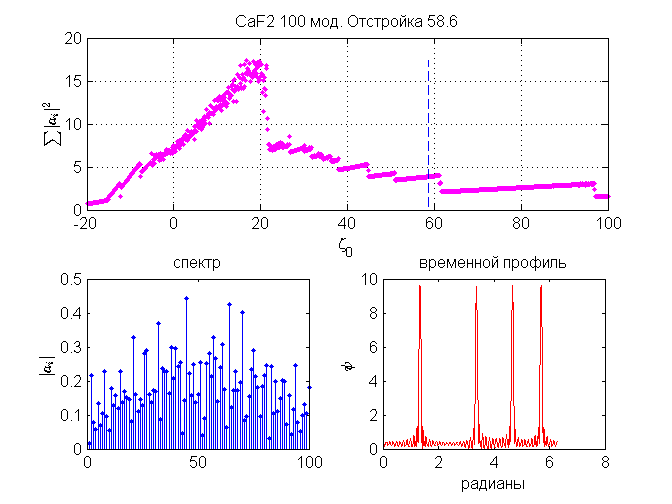
\includegraphics[width = 1\textwidth,height=0.5\textheight]{caf2_main}
 % 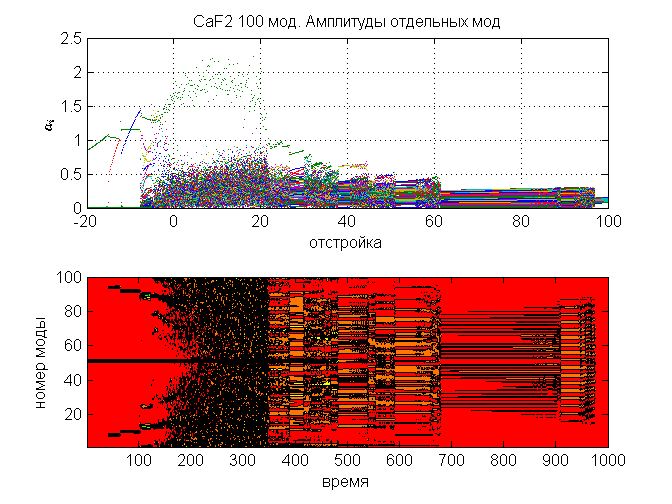
\includegraphics[width = 1\textwidth,height=0.5\textheight]{caf2_modes}
  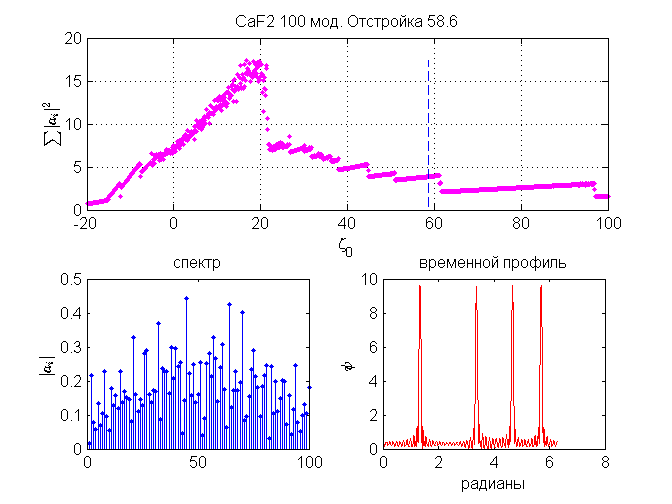
\includegraphics[width = 0.5\textwidth]{caf2_main}
  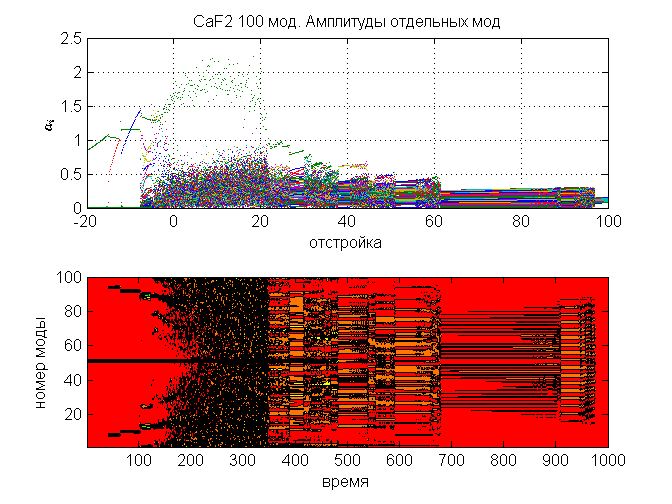
\includegraphics[width = 0.5\textwidth]{caf2_modes}
  \caption{Моделирование 100 мод. Резонатор $CaF_2$. Генерация гребенки в широком диапазоне перестройки лазера} \label{caf2}
\end{figure}

Рассмотрим параметры резонатора, в котором наблюдалась частотная гребенка шириной больше октавы. Рис. \ref{sio2} получен по результатам моделирования для резонатора из $SiO_2$ с параметрами из статьи \cite{DelHaye2011} :
$
Q_0=Q_c=2.7\times10^8,\quad
P_0=2.5\text{ Вт},\quad
\lambda_0=1.56\text{ мкм}, \quad
n_0=1.44,\quad
V_0=5\times10^{-13}\text{ м}^3,\quad
n_2=2.2\times10^{-20}\frac{\text{м}^2}{\text{Вт}},\quad
D_2=10\times10^6\text{ Гц},\quad
D_3=0.$

Резонатор отличается большим $D_2$, мощностью накачки и ОСД. На рисунках видна генерация гребенки в узком диапазоне перестройки лазера. Из-за большой ОСД 200 мод уже покрывают октаву. Результаты моделирования согласуются с выводами авторов статьи.

\begin{figure}
%  \centering
%  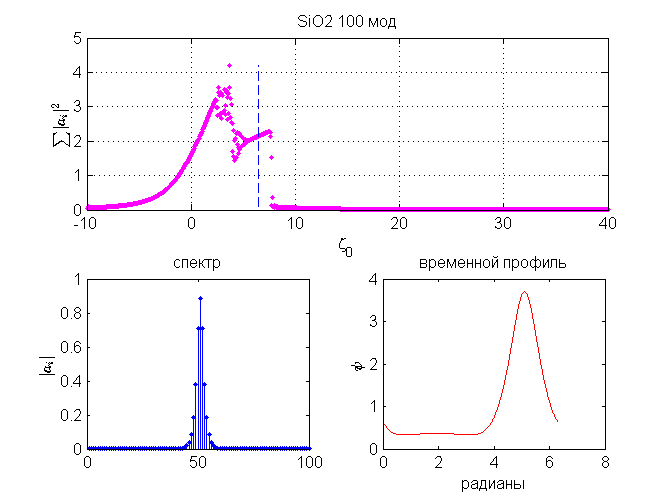
\includegraphics[width = 1\textwidth,height=0.5\textheight]{sio2_100}
 % 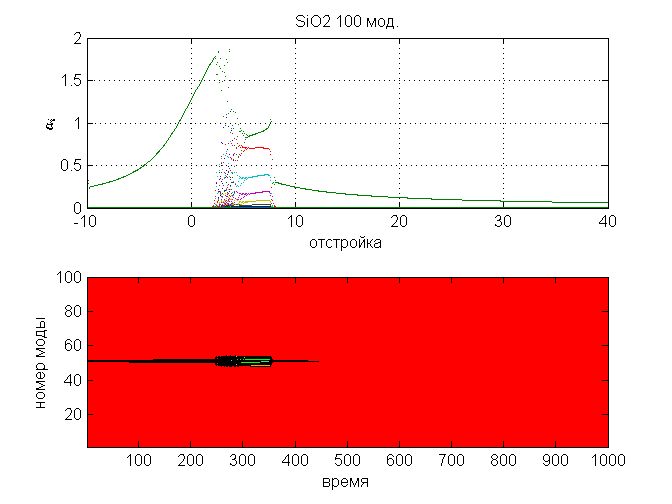
\includegraphics[width = 1\textwidth,height=0.5\textheight]{sio2_100_modal}
  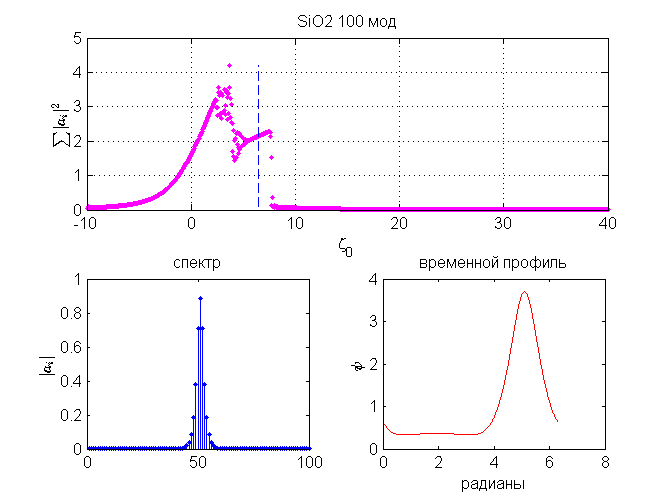
\includegraphics[width = 0.5\textwidth]{sio2_100}
  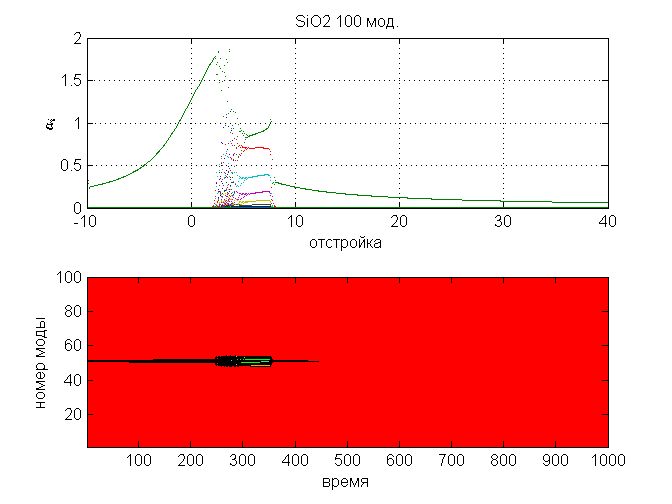
\includegraphics[width = 0.5\textwidth]{sio2_100_modal}
  \caption{Моделирование 100 мод. Резонатор $SiO_2$} \label{sio2}
\end{figure}

\subsection{Сравнение моделирования разными методами}

Для обоснованного использования методов проведем сравнение моделирования системы связанных уравнений с различной правой частью: прямым вычислением суммы или использованием Фурье преобразования \ref{wabnitz_summation}. Рассмотрим резонатор из $MgF_2$ с параметрами из статьи\cite{Herr2014}, см. пункт \ref{subsection_experiment}. Зададим одинаковые параметры резонатора и области перестройки лазера накачки (от $-15$ до $35$ единиц ширины резонанса, счет для $500$ мод). Полученные результаты приведены на рис. \ref{comparison_sum_ft}. Области и режимы генерации совпадают (на верхних графиках). Видны несовпадения в количестве солитонов ($1$ и $3$ соответственно), это объясняется чувствительностью моделирования к начальным шумам в каждой моде. При повторных симуляциях с одинаковым начальным условием количество солитонов совпадало.
\begin{figure}
  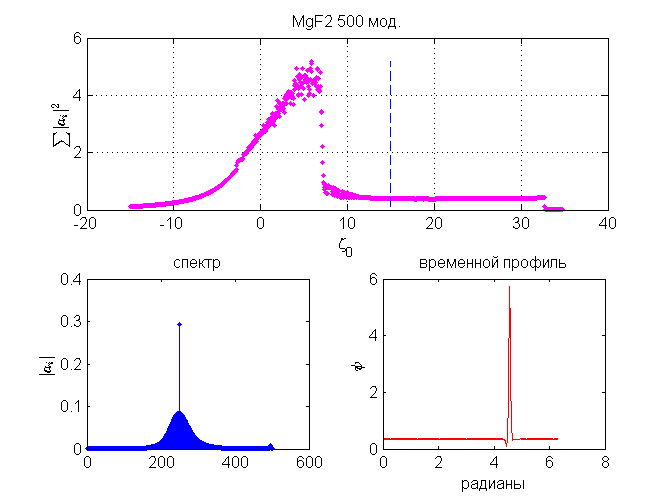
\includegraphics[width = 0.5\textwidth]{mgf2_500cluster}
  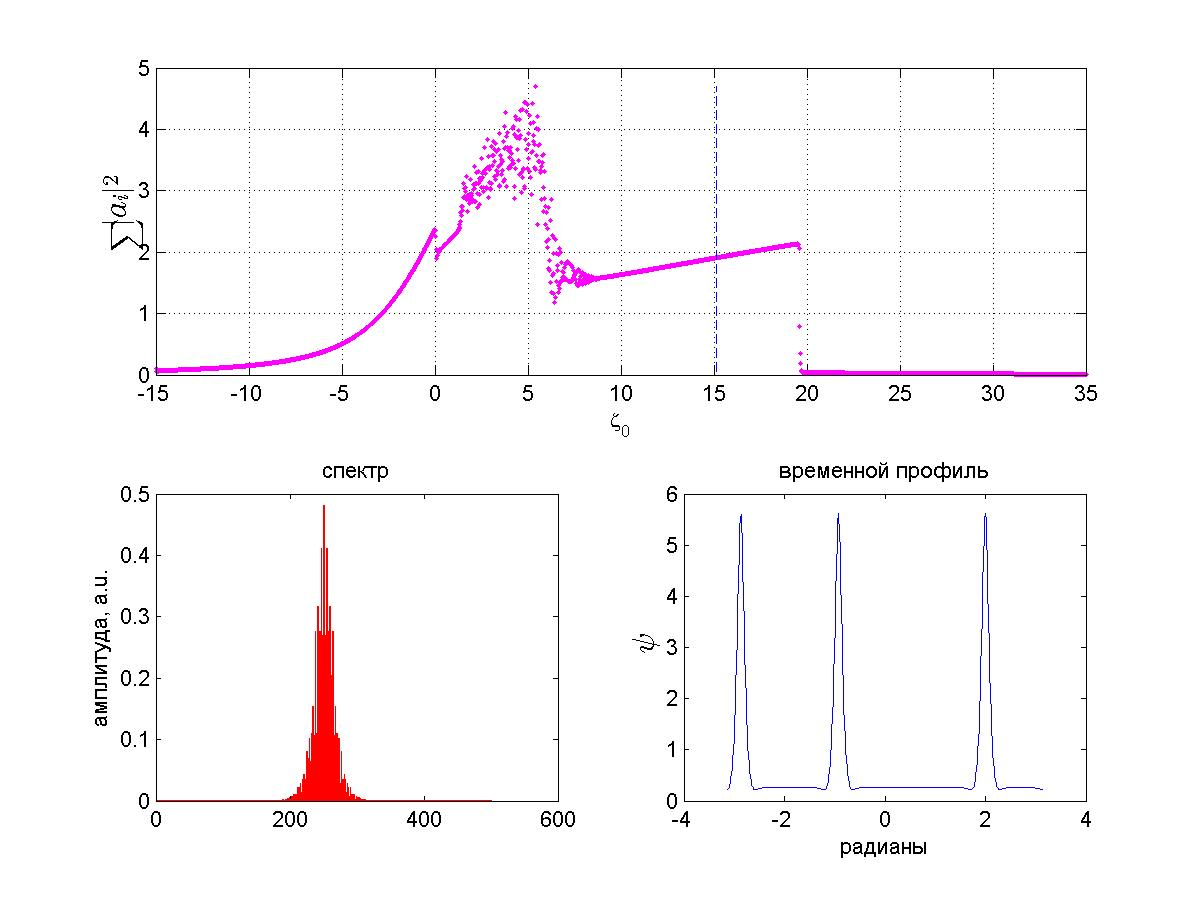
\includegraphics[width = 0.5\textwidth]{mgf2_fft_500}
%  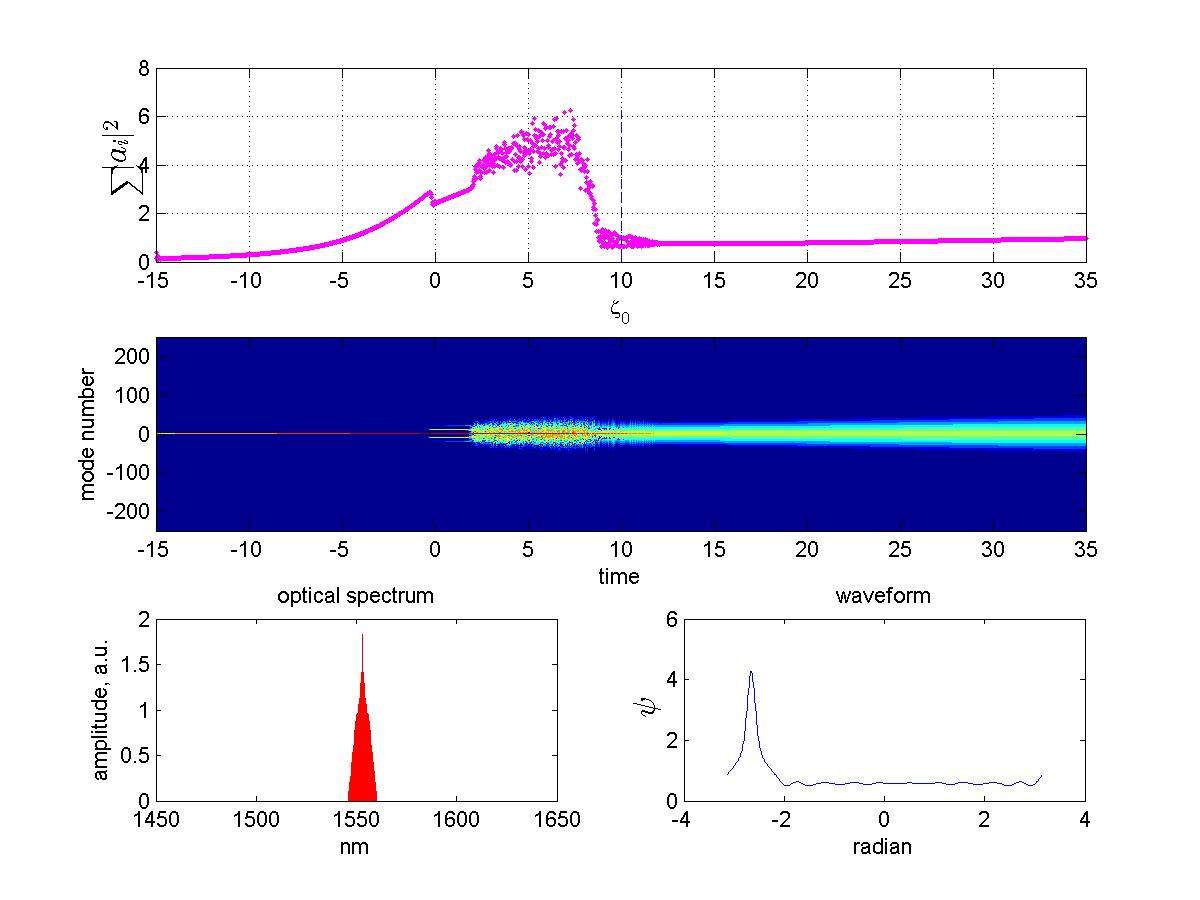
\includegraphics[width = 0.5\textwidth]{mgf2_fft_200}
  \caption{Сравнение методов. Слева счет с прямым суммированием нелинейных членов. Справа с использованием Фурье преобразования. Верхние графики суммы амплитуд мод хорошо совпадают.} \label{comparison_sum_ft}
\end{figure}

Далее сравним результаты моделирования уравнения Луджиато-Лефевера \eqref{LLE} и связанных уравнений в спектральном представлении \eqref{compute_eq}. Зададим одинаковые параметры
$
Q_0=Q_c=5\times10^8,\quad
P_0=100\text{ мВт},\quad
\lambda_0=1.553\text{ мкм},\quad
\omega_0=1.213\times10^{15}\text{ Гц},\quad
n_0=1.376,\quad
V_0=5.6\times10^{-13}\text{ м}^3,\quad
\kappa=\frac{\omega}{Q_0}=1.2\times10^6\text{ Гц},\quad
n_2=0.9\times10^{-20},\quad
g=6.1\times10^{-4},\quad
D_1=2.21\times10^{11}\text{ Гц},\quad
D_2=6.28\times10^4\text{ Гц},\quad
D_3=0\text{ Гц},\quad
\kappa=1.2\times10^6\text{ Гц}.\quad
$
Будем перестраивать лазер накачки от $-15$ до $35$ единиц. Начальным условием в каждой моде выступает нормально распределенный шум $\mathcal{N}(0,1)$. Результаты показаны на рис. \ref{comparison_coupled_lle}. Картина моделирования методом SSFM хорошо совпадает с картиной для связанных уравнений - последовательно наблюдаются рост только моды накачки, зона модуляционной нестабильности, далее стабильная генерация нескольких импульсов. Основные отличия - количество наблюдаемых импульсов и величина отстройки, при которой частотная гребенка пропадает. При повторных симуляциях при других параметрах число импульсов иногда совпадало. Можно утверждать, что обе математические модели дают хорошее совпадение при описании физического явления генерации частотных гребенок в микрорезонаторах.

\begin{figure}
  %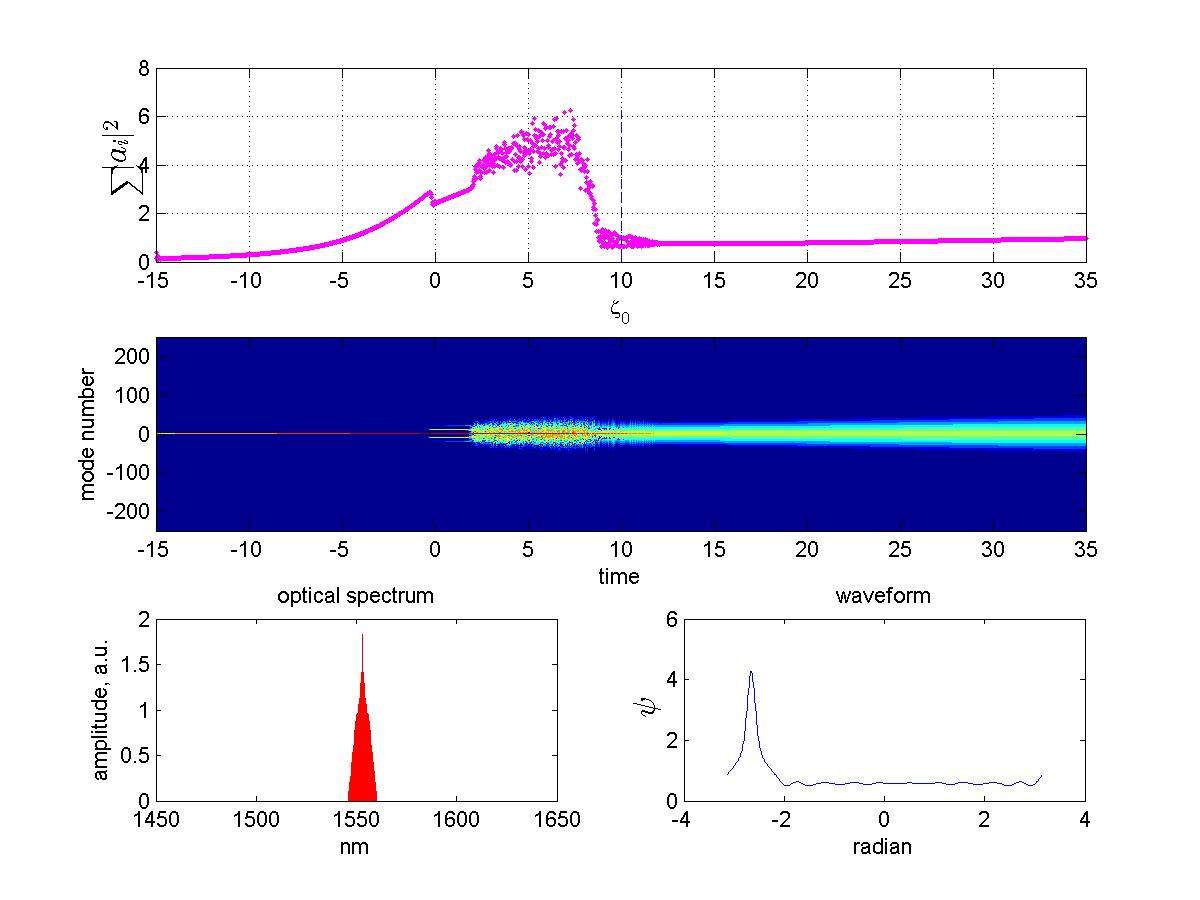
\includegraphics[width = 0.5\textwidth]{mgf2_fft_200}
  %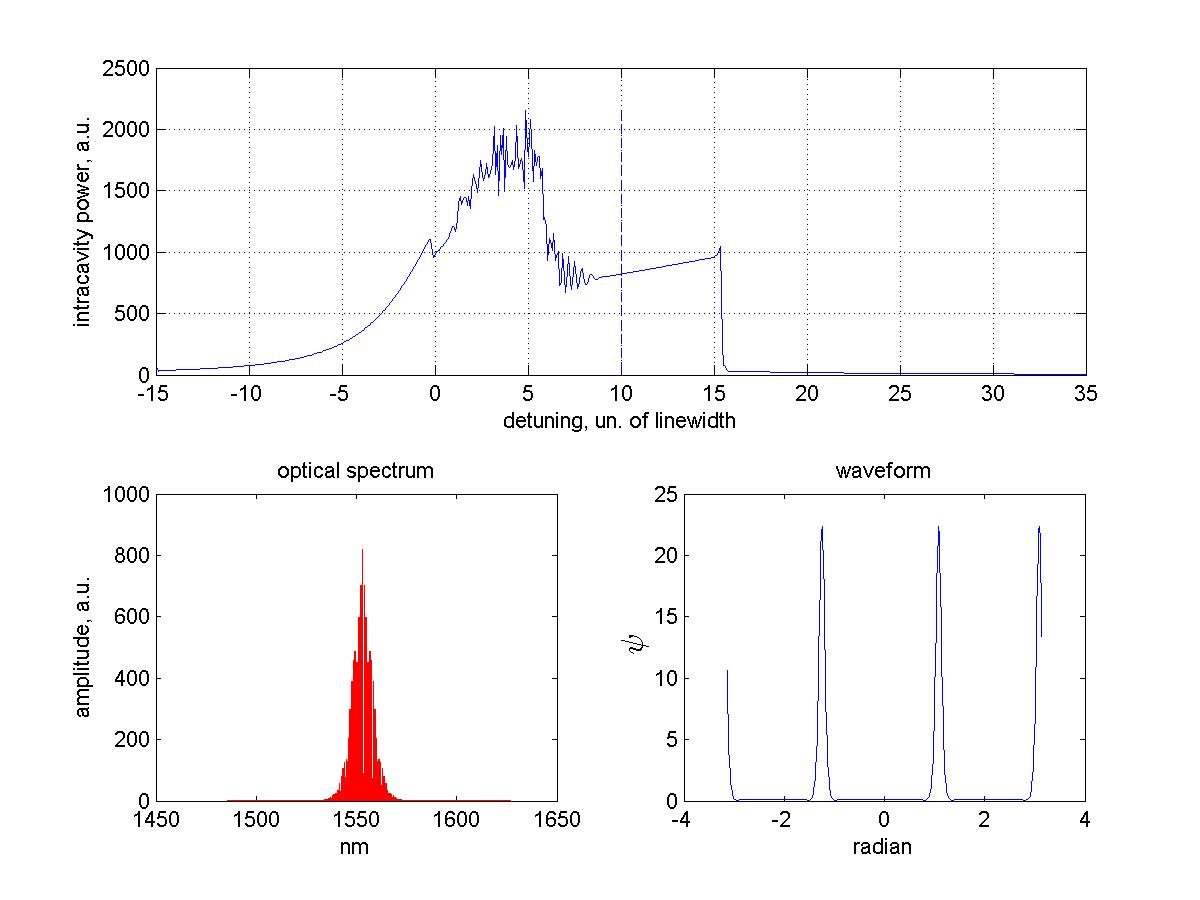
\includegraphics[width = 0.5\textwidth]{mgf2_lle_501}
  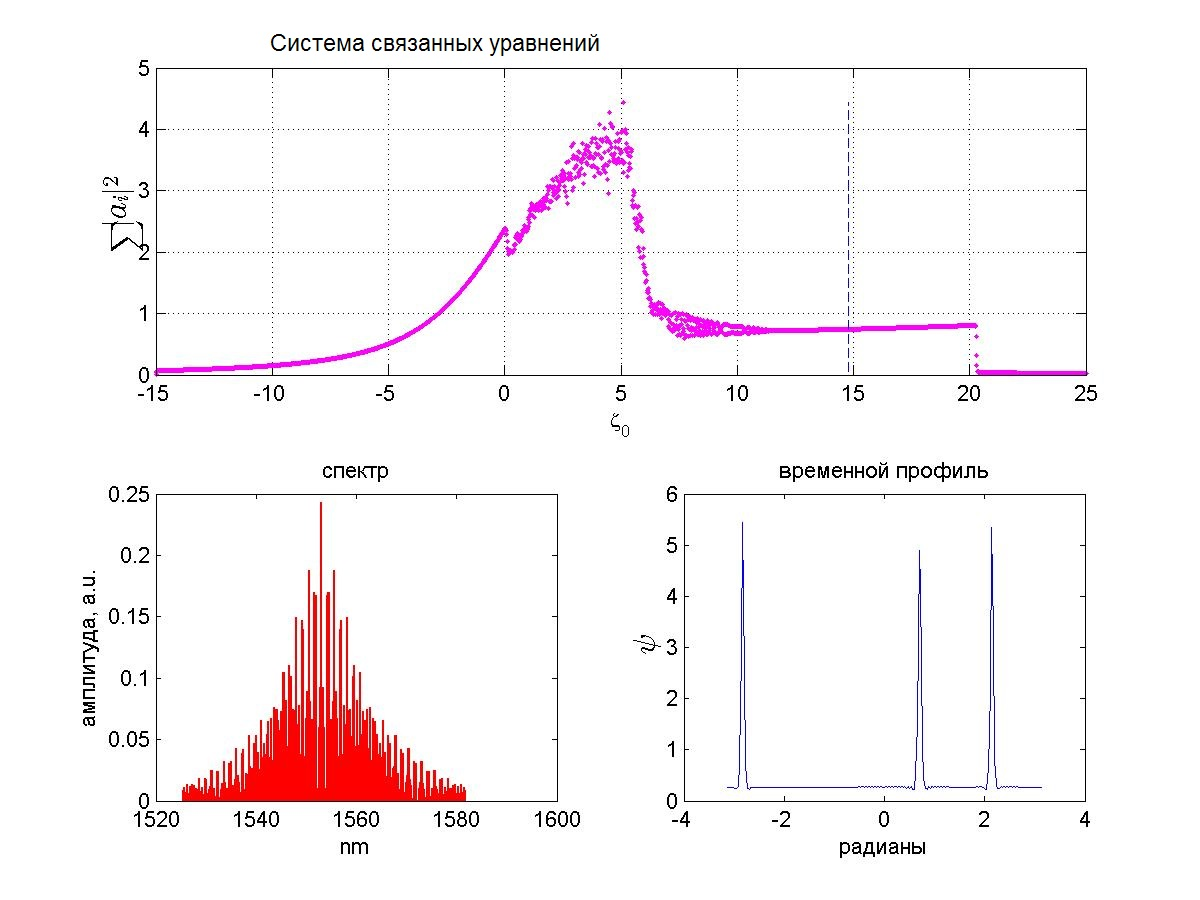
\includegraphics[width = 0.5\textwidth]{mgf2_compare_coupled}
  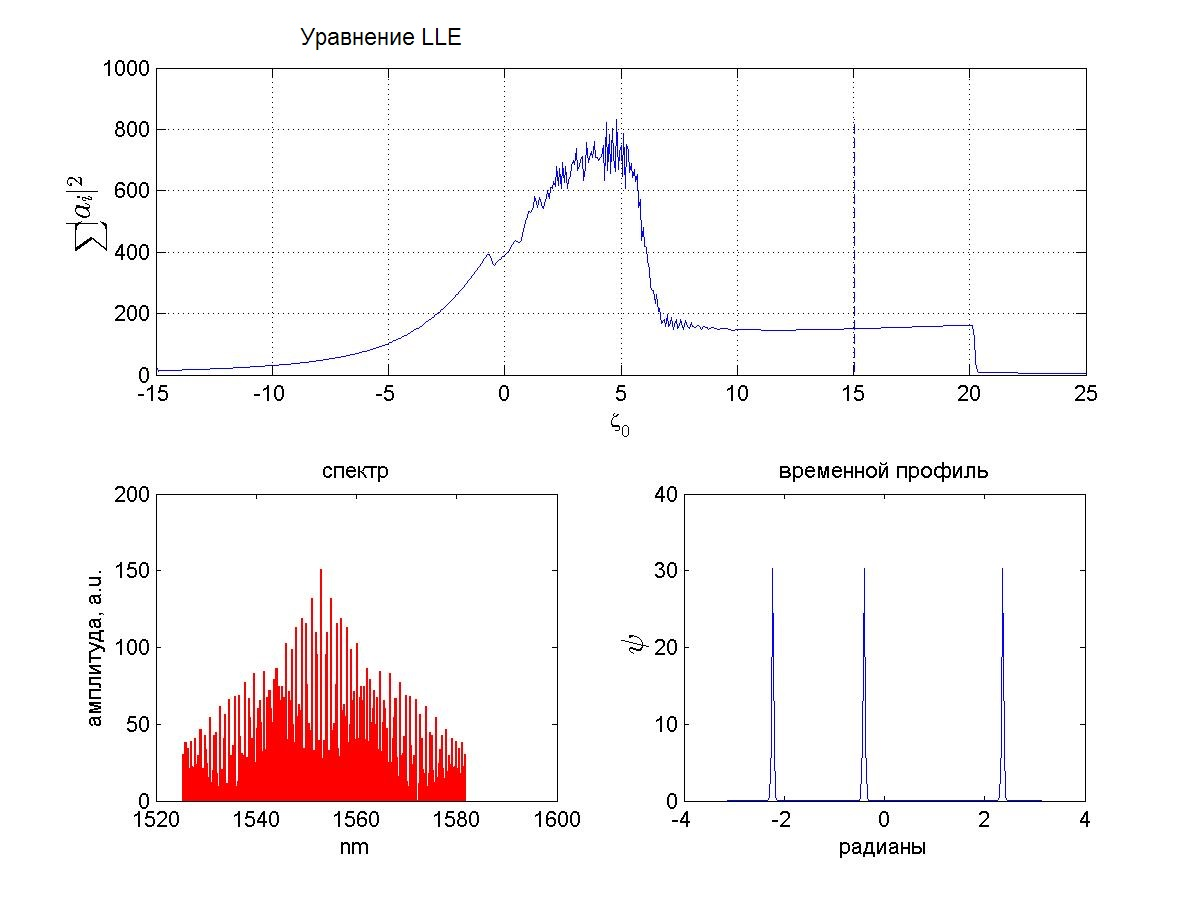
\includegraphics[width = 0.5\textwidth]{mgf2_compare_lle}
  \caption{Сравнение мат. моделей. Слева счет для системы связанных уравнений. Справа для уравнения Луджиато-Лефевера.} \label{comparison_coupled_lle}
\end{figure}

\subsection{Учет нагрева резонатора.}

Для более точного совпадения численного моделирования с экспериментом требуется учет нагрева резонатора лазером накачки, что приводит к другой конфигурации мод и нарушению режима генерации гребенок. К основной системе уравнений \eqref{compute_eq} добавляется уравнение теплопроводности. Следуя \cite{Gorodetsky} получим систему:
\begin{equation}
\frac{\partial a_\mu}{\partial \tau}=-[1+i\zeta_{\mu}-i\Theta]a_\mu+i\sum_{\mu^\prime\le\mu^{\prime\prime}} (2-\delta_{\mu^\prime\mu^{\prime\prime}})a_{\mu^\prime}a_{\mu^{\prime\prime}}a_{\mu^\prime+\mu^{\prime\prime}-\mu}^*+\delta_{0\mu}F,
\end{equation}
\begin{equation}
\frac{\partial \Theta}{\partial \tau}+\frac{2\delta_\theta}{\kappa}\Theta=\frac{n_{2\theta}}{n_2}\frac{2\delta_\theta}{\kappa}\sum_\mu |a_\mu|^2,
\end{equation}
где $\Theta$ - усредненная по объему моды температура.

Выбранная модель предполагает, что сдвиг каждой моды при учете тепловой нелинейности одинаков. Программа была доработана, в связанные уравнения добавлена зависимость отстройки от $\Theta$, вычисление $\Theta$ производилось на каждом шаге по времени. Выбрано отношение $\frac{2\delta_\theta}{\kappa}=20$.  Рис. \ref{therm} дает результат моделирования с учетом небольшого теплового коэффициента $n_{2\theta}=10$, остальные параметры резонатора $MgF_2$ были приведены в предыдущих пунктах.

Был применен новый сценарий - лазер перестраивался от $-15$ до $50$ единиц и далее оставался на отстройке $50$ до конца симуляции. Видно, что генерация гребенки сохраняется, но диапазон требуемой перестройки лазера заметно увеличивается. При численном моделировании удается зафиксировать многосолитонный режим. Однако во всех реальных экспериментах для фиксации такого режима используются различные механизмы тепловой стабилизации.

\begin{figure}
  %\centering
  %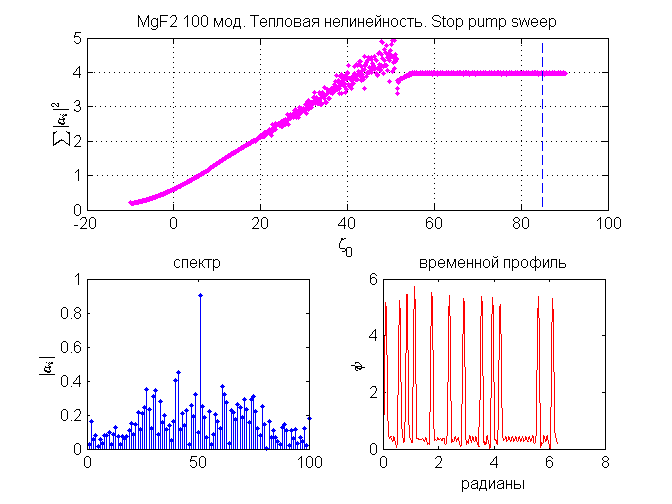
\includegraphics[width = 1\textwidth,height=0.5\textheight]{mgf2_therm_stop_detune}
  %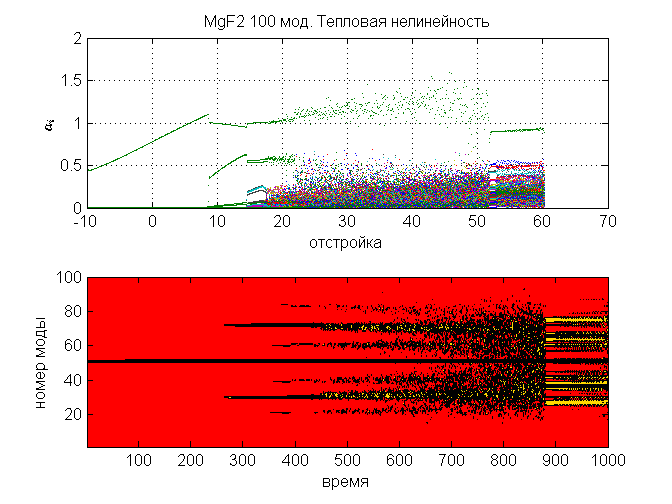
\includegraphics[width = 1\textwidth,height=0.5\textheight]{mgf2_therm_good_modes}
  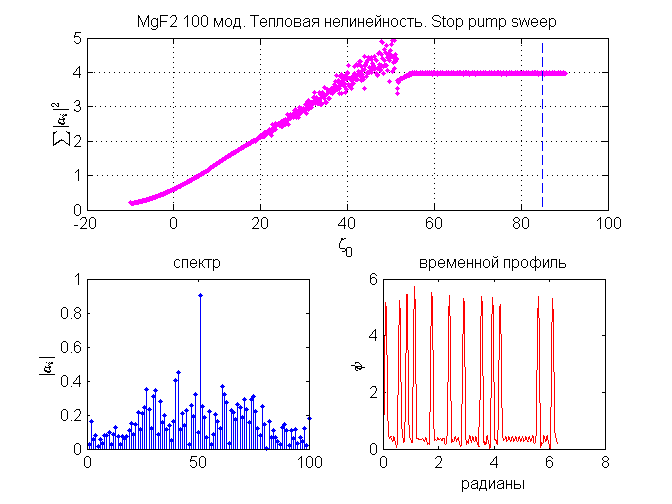
\includegraphics[width = 0.5\textwidth]{mgf2_therm_stop_detune}
  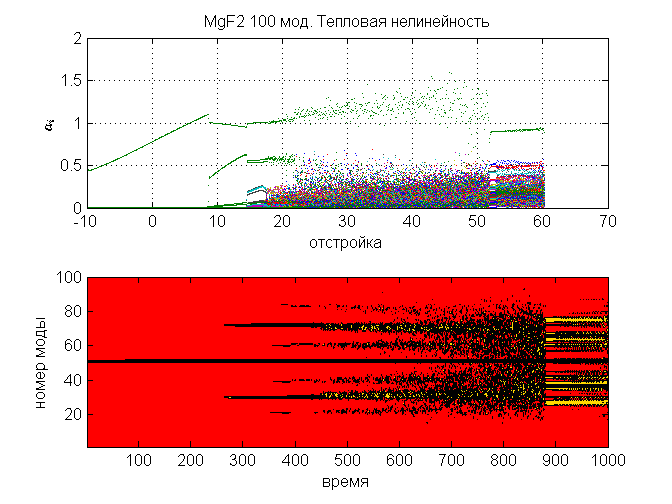
\includegraphics[width = 0.5\textwidth]{mgf2_therm_good_modes}
  \caption{Резонатор из $MgF_2$. Слабая тепловая нелинейность. Фиксация многосолитонного режима происходит при остановке перестройки лазера накачки на $50$} \label{therm}
\end{figure}

\subsection{Отсутствие генерации гребенки.}
Не во всех лабораториях удавалось экспериментально наблюдать солитонный режим. В некоторых случаях возбужденными оказывались лишь небольшое число боковых мод. Приведем сценарии, когда частотная гребенка не наблюдалась и при численном моделировании.

На рис. \ref{no_comb} вверху показан результат для резонатора из $MgF_2$ при большой тепловой нелинейности $n_{2\theta}=100$. Боковые моды не возбуждаются в широком диапазоне перестройки (проводилась симуляция от $-20$ до $100$ единиц).

На рис. \ref{no_comb} внизу показан сценарий одновременной перестройки и линейного увеличения мощности накачки от 0 до $P_0=100$ мВт. Боковые моды не возбуждались.

Был рассмотрен сценарий, когда лазер отстроен на фиксированную величину $10$, его мощность линейно увеличивается от 0 до $P_0=100$ мВт. Оптическая гребенка в этом случае не наблюдалась.

Гребенка также не наблюдалась при малых значениях добротности $Q\approx10^5$ или больших значениях $D_2\approx10^7$ Гц.

\begin{figure}
  %\centering
  %  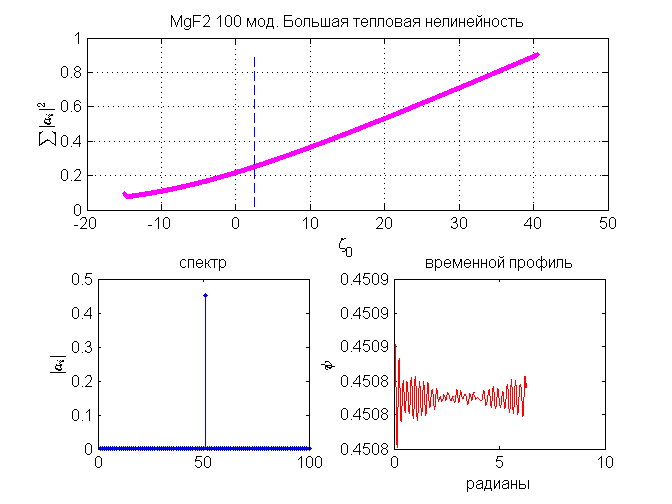
\includegraphics[width = 1\textwidth,height=0.5\textheight]{mgf2_big_therm}
 % 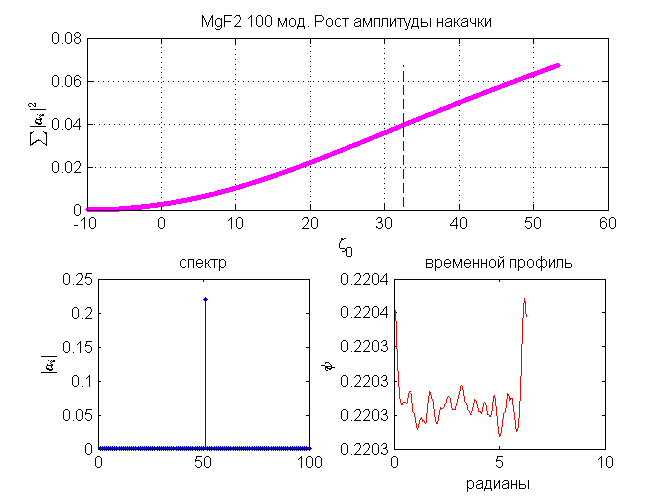
\includegraphics[width = 1\textwidth,height=0.5\textheight]{mgf2_f_grow_therm}
  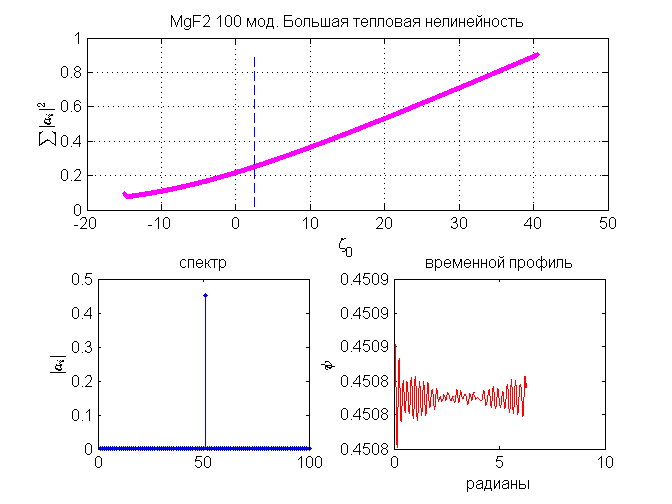
\includegraphics[width = 0.5\textwidth]{mgf2_big_therm}
  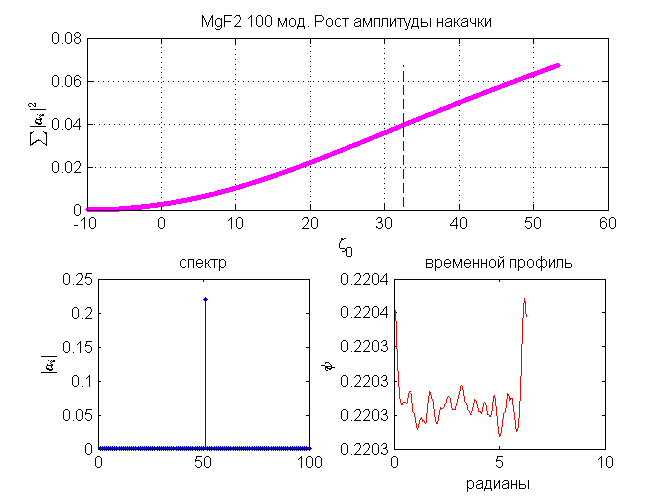
\includegraphics[width = 0.5\textwidth]{mgf2_f_grow_therm}
  \caption{Отсутствие гребенки. Резонатор из $MgF_2$. Большая тепловая нелинейность (слева). Рост мощности накачки (справа)} \label{no_comb}
\end{figure}

\subsection{Различные сценарии моделирования}

Для резонатора из $MgF_2$ моделировались сценарии фиксации солитонного режима. Рис. \ref{step_detune} дает зависимости: а) лазер равномерно перестраивается и останавливается на отстройке, соответствующей солитонному режиму; б) лазер перестраивается скачком с отстройки, соответствующей хаотическому режиму, на отстройку, соответствующую солитонному режиму (режим рассмотрен в \cite{Matsko2013}). В обоих случаях симуляция давала желаемый результат - фиксацию солитонного режима. Однако в эксперименте этому препятствует большая тепловая нелинейность.

\begin{figure}
%  \centering
%  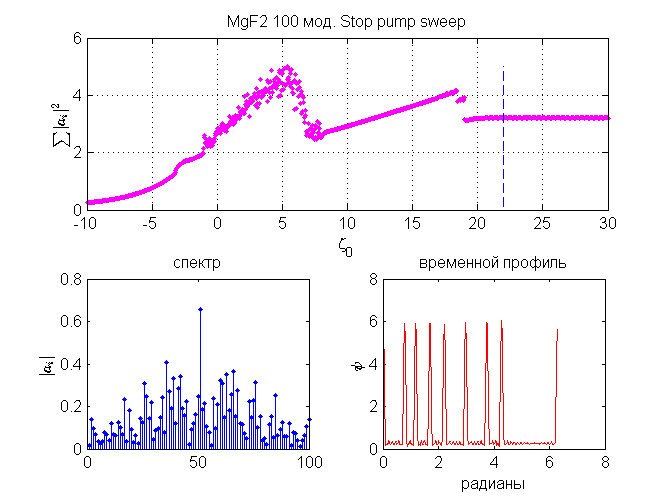
\includegraphics[width = 1\textwidth,height=0.5\textheight]{mgf2_stop_pump_sweep}
 % 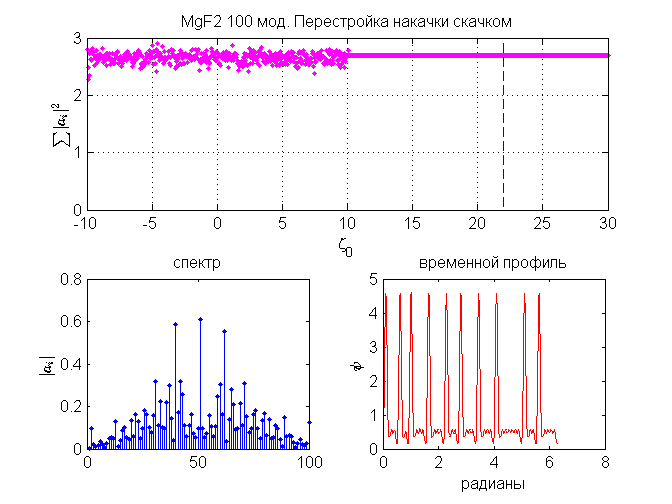
\includegraphics[width = 1\textwidth,height=0.5\textheight]{step_detune_main}
  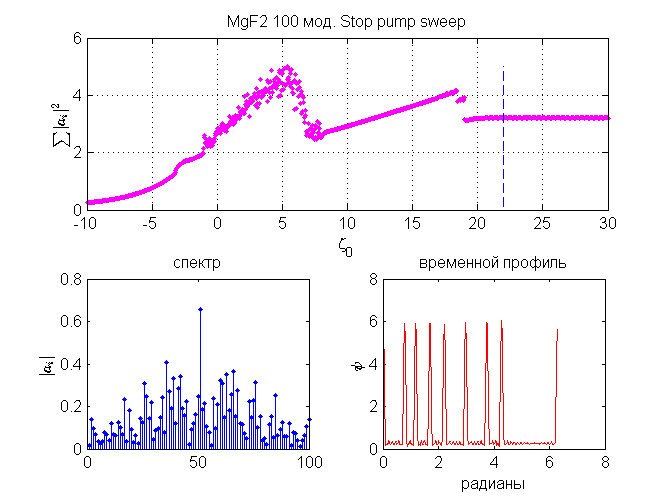
\includegraphics[width = 0.5\textwidth]{mgf2_stop_pump_sweep}
  \includegraphics[width = 0.5\textwidth]{step_detune_main}
  \caption{Фиксация солитонного режима. Остановка перестройки лазера накачки (слева). Перестройка скачком (справа)} \label{step_detune}
\end{figure}

С экспериментальной точки зрения интересен сценарий сдвига собственной частоты моды накачки на постоянную величину от соседних мод. Рисунок \ref{pump_shift} показывает динамику гребенки в зависимости от сдвига центральной частоты моды накачки. Тем самым моделируется отклонение от разложения $\omega_\mu=\omega_0+D_1\mu+\frac{1}{2}D_2\mu^2$ в нулевой точке. Сдвиг выражен в единицах ширины резонансной кривой. При больших сдвигах в положительную или отрицательную сторону гребенка не генерируется (при сохранении аномальной дисперсии).

\begin{figure}
  \centering
  \includegraphics[width = 1\textwidth,height=0.5\textheight]{pump_shift_plus}
  \includegraphics[width = 1\textwidth,height=0.5\textheight]{pump_shift_minus}
  \caption{Измененный закон дисперсии: сдвиг частоты моды накачки в единицах ширины резонансной кривой} \label{pump_shift}
\end{figure}

Другим интересным для эксперимента параметром является фазовая модуляция лазера накачки. В спектральном представлении фазовая модуляция эквивалентна возбуждению боковых мод. В программу были внесены изменения -  помимо центральной моды подавалась постоянная накачка разного знака в $2$ соседние моды. Рис. \ref{phase_pump} показывает результат моделирования - генерация гребенки сохраняется, на графике амплитуд отдельных мод видна их осциллирующая форма. Однако при увеличении накачки в боковые моды (соответственно глубины фазовой модуляции) пропадают области многосолитонного режима.

\begin{figure}
%  \centering
%  \includegraphics[width = 1\textwidth,height=0.5\textheight]{phase_pump}
 % \includegraphics[width = 1\textwidth,height=0.5\textheight]{phase_pump_modal}
  \includegraphics[width = 0.5\textwidth]{phase_pump}
  \includegraphics[width = 0.5\textwidth]{phase_pump_modal}
  \caption{Фазовая модуляция накачки} \label{phase_pump}
\end{figure}

\subsection{Влияние дисперсии резонатора}

В экспериментальных работах исследуется влияние дисперсии высоких порядков на формирование частотной гребенки. Рассмотрим разложение $\omega_\mu=\omega_0+D_1\mu+\frac{1}{2}D_2\mu^2+\frac{1}{6}D_3\mu^3$. Дисперсия второго порядка $D_2=-\frac{c}{n}D_1^2\beta_2$, где $\beta_2$ - дисперсия групповой скорости. Положительная $D_2$ соответствует аномальной дисперсии резонатора и параболическому отличию распределения мод от эквидистантности. Коэффициенты $D_2, D_3$ оцениваются аналитически или численно, учитывая материальную и геометрическую дисперсии. Для резонатора из $MgF_2$ проведем моделирование для разных значений этих параметров. Результаты представлены на рис. \ref{d2d3_plot}. Цветом дано отношение пиковой и средней мощности внутри резонатора. Оно выступает как индикатор количества солитонов, максимальное значение соответствует односолитонному режиму. Картина симметрична для положительных и отрицательных $D_3$. Минимальное число солитонов достигается при устремлении $D_3\rightarrow 0$ и небольших $D_2\ge0$.

\begin{figure}
  \centering
  \includegraphics[scale = 0.5]{d2d340p40}
  \caption{Резонатор из $MgF_2$. Зависимость числа генерируемых солитонов от дисперсии второго и третьего порядка. Цветовая шкала показывает отношение пиковой и средней мощности внутри резонатора. Максимальное значение (красный цвет) соответствует односолитонному режиму. Меньшие значения (синий цвет) соответствуют многосолитонным режимам и режимам без генерации солитонов.} \label{d2d3_plot}
\end{figure}

Далее было выполнено моделирование отклонения от параболического вида $\omega_\mu-\omega_0-D_1\mu=\frac{1}{2}D_2\mu^2$ путем добавления случайного шума в каждую моду с нормальным распределением. Случайная величина с гауссовским распределением $\mathcal{N}(0,1)$ получалась из случайных величин с равномерным распределением по алгоритму Box-Muller \cite{Press2002}. На рис. \ref{gaus} приведены графики динамики гребенки при заданном распределении мод по частоте (отклонению от эквидистантности). Увеличивая дисперсию шума, мы сужаем области многосолитонного режима. Однако последний график показывает, что даже при значительных отклонениях от параболического вида для удаленных мод, но при сохранении такового для близких к центральной моде накачки, хорошо наблюдается гребенка с солитонными режимами.

\begin{figure}
  \centering
%  \includegraphics[width = 1\textwidth,height=0.5\textheight]{gaus1}
  \includegraphics[width = 1\textwidth,height=0.5\textheight]{gaus2}
  \caption{Отклонение от параболического разложения \eqref{dispersion_eq} для мод. Цветовая шкала показывает отношение пиковой и средней мощности внутри резонатора. Максимальное значение (красный цвет) соответствует односолитонному режиму. Меньшие значения (синий цвет) соответствуют многосолитонным режимам и режимам без генерации солитонов.} \label{gaus}
\end{figure}

Известно, что связь между семействами мод в резонаторе дополнительно изменяет собственные частоты и может приводить к особой картине пересечения мод \cite{HerrPRL2014}. В упрощенной модели эффект нормального расщепления мод может быть параметризован как гиперболическое отличие распределения мод $\omega_\mu=\omega_0+D_1\mu+\frac{1}{2}D_2\mu^2+\frac{a/2}{\mu-b-0.5}$, где $a$ показывает на сколько выбивается мода с номером $b$. Результат моделирования для различных $a,b$ приведен на рис. \ref{offsetplot}. Картина центрально-симметричная, видно, что даже небольшие выбивания близких к центральной мод приводят к картине без солитонов. Этот результат согласуется с ранними экспериментальными данными \cite{HerrPRL2014}. Однако позже мною экспериментально неоднократно замечалось, что наличие расщепления моды накачки, приводит к уширению солитонной ступеньки. При дальнейшей настройке на солитонный режим, наблюдалось большое число дисперсионных волн на эффектах нормального расщепления мод, сигнал биений на частоте повторения солитона был шумным (порядка 10 кГц). Иногда наблюдалась одновременная параметрическая генерация отдельных линий на другом семействе мод, т.ч. фактически один лазер генерировал гребенки на двух семействах мод при накачке в месте их пересечения.

\begin{figure}
  \centering
  \includegraphics[width = 0.8\textwidth]{offsetplot}

  \includegraphics[width = 0.2\textwidth]{mode_crossing}
%  \includegraphics[scale = 0.5]{offsetplot}
 % \includegraphics[width = 0.3\textwidth]{mode_crossing}
  \caption{Резонатор из $MgF_2$. Гиперболическое отличие частот в законе дисперсии. Параметр $a$ показывает на сколько выбивается мода с номером $b$. Цветовая шкала дает отношение пиковой и средней мощности внутри резонатора. Максимальное значение соответствует односолитонному режиму} \label{offsetplot}
\end{figure}

\subsection{Моделирование генерации дисперсионной волны по экспериментальным данным}

В эксперименте \cite{Brasch2016} впервые экспериментально продемонстрирован оптический временной солитон и индуцированная им дисперсионная волна в интегральном микрорезонаторе из $Si_3N_4$ \ref{brashch_dispersive_wave}. При наличии дисперсии высоких порядков оптический солитон может излучать дисперсионную волну \cite{PhysRevA.51.2602} вблизи частот с нулевой суммарной дисперсией. Хотя в волоконной оптике этот эффект считается вредным для некоторых приложений, для микрорезонаторов он позволил расширить спектральное покрытие гребенки и при правильном выборе геометрии резонатора дает мощные пики по краям спектра, необходимые при удвоении частоты для самосинхронизации f-2f \cite{Spencer2018}. При наличии дисперсии третьего и более высоких порядков спектр возмущенного солитона перестает быть симметричным, максимум спектра сдвигается и возникает дополнительный мощный спектральный пик. Во временном представлении солитон имеет осциллирующий хвост (отсюда другое название по аналогии: оптическое черенковское излучение). Положение спектрального пика определяется из условия нуля суммарной дисперсии: $\mu_{dw}=\frac{-3D_2}{D_3}$ при $D_4=0$ и $\mu_{dw}=\frac{-2D_3}{D_4}\pm\sqrt{(\frac{2D_3}{D_4})^2-\frac{12D_2}{D_4}}$ при $D_4\neq0$.

Было проведено численное моделирование по параметрам, полученным из экспериментальных данных по измерению дисперсии в диапазоне вблизи накачки ($D_3,D_4$ подбирались вручную): $D_2/2\pi=2.2$ МГц, $D_3/2\pi=25$ кГц, $D_4/2\pi=-300$ Гц. Мощность накачки 1 Вт, добротность $Q=10^6$. Начальным условием являлся односолитонный режим, полученный из набора предыдущих симуляций. Эффективная отстройка составила $\zeta=12$ для наилучшего совпадения с экспериментом.  Вычисленное значение $\mu_{dw}=-200$, что близко к экспериментальному значению -195. На рис. \ref{brashch_dispersive_wave} зеленым показана огибающая спектра, полученная при моделировании, видно хорошее совпадение по мощности линий, но с общим сдвигом. Отсутствие в эксперименте сдвига максимума огибающей спектра связано с тем, что в нитриде кремния одновременно происходит сдвиг спектрального максимума в противоположную сторону из-за эффекта Рамана \cite{Karpov2016}, а также из-за не учитываемой в моделировании зависимости нелинейного коэффициента $\gamma$ от частоты.

\begin{figure}
  \centering
  \includegraphics[width = 0.9\textwidth]{brashch_dispersive_wave}

  \caption{А: оптический временной солитон и индуцированная им дисперсионная волна в интегральном микрорезонаторе из $Si_3N_4$, зеленым дана огибающая гребенки из численного моделирования по параметрам из эксперимента; В: дисперсионная кривая микрорезонатора, вычисленная методом FEM моделирования с нанесенными экспериментальными точками.} \label{brashch_dispersive_wave}
\end{figure}


\subsection{Моделирование уравнения Луджиато-Лефевера методом конечных разностей}

Моделирование уравнения LLE \eqref{LLE} c начальным профилем
\begin{equation} \label{initial_cond_soliton}
\psi(0,\theta)=\sqrt{2\zeta_0}\exp (i \arccos(\frac{\sqrt{8\zeta_0}}{\pi f}))\sum_j sech(\sqrt{\frac{\zeta_0}{d_2}}(\theta-\theta_j))
\end{equation}
было проведено в пакете Mathematica. Использовалась функция NDSolve, которая реализует конечно-разностный метод. Для одного солитона методом проб и ошибок были найдены границы изменений параметров $\zeta_0,f$, при которых солитон распространяется без изменения профиля.
%(представлены на рис. \ref{nls}).

Для многосолитонных профилей удалось проследить, как, изменяя ширину и расстояние между солитонами, удается добиться распространения без столкновений за длительное время (рис. \ref{2solitons},\ref{3solitons})
\begin{figure}
  \includegraphics[width = 0.5\textwidth,height=0.25\textheight]{2solitons_gap1}
  \includegraphics[width = 0.5\textwidth,height=0.25\textheight]{2solitons_gap2}
\end{figure}

\begin{figure}
  \includegraphics[width = 0.5\textwidth,height=0.25\textheight]{2solitons_gap4}
  \includegraphics[width = 0.5\textwidth,height=0.25\textheight]{2solitons_gap6}
  \caption{Столкновение двух солитонов. Увеличивая начальное расстояние между солитонами, можно добиться отсутствия столкновения.} \label{2solitons}
\end{figure}

\begin{figure}

  \includegraphics[width = 0.5\textwidth]{3solitons_gap6}
  \includegraphics[width = 0.5\textwidth]{3solitons_gap12}
  \caption{Столкновение трех солитонов. Увеличивая начальное расстояние между солитонами, можно добиться отсутствия столкновения.} \label{3solitons}
\end{figure}


\section{Моделирование возбуждения оптических частотных гребенок и платиконов в микрорезонаторах с нормальной дисперсией групповой скорости}

Достичь в микрорезонаторах аномальной суммарной дисперсии групповой скорости (ДГС) в широкой полосе частот для произвольной центральной частоты сложно, т.к. материальная ДГС в видимом и ближнем ИК диапазонах в основном нормальная и большая по модулю, т.ч. компенсировать ее подбором геометрии резонатора сложно. Поэтому необходимо найти пути генерации оптических частотных гребенок при нормальной дисперсии.

Известно, что в реальных микрорезонаторах наблюдаемые дисперсионные соотношения могут существенно отличаться от теоретических, например, из-за наличия связи между различными семействами мод. В частности, это может приводить к существенному сдвигу резонансных частот. Благодаря этому закон дисперсии вблизи “сдвинутой” моды может характеризоваться наличием локальной эффективной аномальной дисперсии, что в свою очередь является причиной появления модуляционной неустойчивости, приводящей к дальнейшему возбуждению частотной гребенки с светлыми или темными солитонами.

С помощью численного моделирования будет показано, что если сдвинута накачиваемая лазером мода резонатора, либо из-за эффекта нормального расщепления мод, либо в результате сильного эффекта затягивания, то возможна генерация стабильных ультракоротких импульсов с плоской вершиной, которые назовем платиконами. Будет показано, что если такое выбивание моды достаточно большое (величиной в несколько ширин линий моды резонатора), тогда платиконы могут быть сгенерированы спонтанно, когда лазер перестраивается через эффективную нулевую отстройку высокодобротного резонанса. Длительность таких сгенерированных импульсов можно непрерывно менять, изменяя отстройку лазера накачки от резонанса.

Моделирование было проведено для системы связанных уравнений:
%
\begin{equation}
\frac{\partial a_\mu}{\partial \tau}=-[1+i\zeta_{\mu}]a_\mu+i\sum_{\mu^\prime,\mu^{\prime\prime}} a_{\mu^\prime}a_{\mu^{\prime\prime}}a_{\mu^\prime+\mu^{\prime\prime}-\mu}^*+\delta_{0\mu}f,
\end{equation}

Для анализа использовалось разложение дисперсионного закона в ряд Тэйлора до 2 порядка, дисперсией более высокого порядка не учитывались $\omega_\mu=\tilde\omega_0-\delta_{0\mu}\Delta+D_1\mu+\frac{1}{2}D_2\mu^2$,  где $\tilde\omega_0$ не возмущенная частота моды накачки, $\Delta$ описывает интересующий сдвиг моды накачки и $\delta_{0\mu}$ символ Кронекера. Для нормальной дисперсии $D_2<0$.

Для моделирования использовались следующие параметры MgF$_2$ микрорезонатора: длина волны $\lambda=2\pi c/\omega_0=1.5$ $\mu$m, $n_0=1.37$, $n_2=0.9\times 10^{-20}$ m$^2$/W, $V_{\mathrm{eff}}=5.6\times 10^{-13}$m$^3$,  $Q_0=Q_\text{ext}=4\times 10^8$, $D_2/(2\pi)=-10$kHz. Мощность накачки $P_\mathrm{in}=50$mW соответсвует приблизительно $f\approx 4.11$. Численно было проверено, что качественно похожие результаты получаются и для параметров резонатора из нитрида кремния\cite{Brasch2016}.

Система уравнений решалась численно с помощью адаптивного метода Рунге-Кутта для 501 моды. В качестве начального условия генерировалось слабая шумоподобная затравка (на уровне вакуумных флуктуаций). Для анализа рассчитывалась усредненная интенсивность внутри микрорезонатора $U=\sum_\mu |a_\mu|^2$ и распределение поля $\psi(\phi)=\sum_\mu a_\mu \exp(i\mu\phi)$, где $\phi$ азимутальный угол.

Для моделирования процесса генерации солитонов при перестройке частоты накачки расстройка $\zeta_0$ медленно менялась со временем от отрицательной величины $\zeta_0(0)=-20$, соответствующей отстройке накачки в синюю область, до значительной положительной величины.  При отсутствии или отрицательной величине сдвига моды накачки наблюдался характерная картина треугольного резонанса, соответствующая простому одночастотному решению. Однако при наличии существенного сдвига моды накачки в резонансной характеристике $U(\zeta_0)$ появлялась характерная ступенька, сигнализирующая о переходе в режим генерации импульсов Рис.\ref{platicon_triangles}(а).

\begin{figure}
  \centering
  \includegraphics[width = 1\textwidth,height=0.5\textheight]{triangles}
  \caption{Зависимость усредненной интенсивности внутри микрорезонатора $U$ от нормированной отстройки $\zeta_0$ (a) для различных значений сдвига моды накачки при $f=4.11$ и (в) для различных амплитуд накачки $2\Delta/\kappa=8$} \label{platicon_triangles}
\end{figure}


При остановке перестройки частоты вблизи этой ступеньки солитонный режим сохранялся неограниченное время.
При увеличении мощности накачки “ступенька” становилась более заметной и сдвигалась по частоте к большим значениям расстройки (рис. \ref{platicon_triangles}(б)).

Построенное в таком режиме распределение поля показало наличие локализованных импульсов, обладающих характерным профилем с плоской вершиной (рис. \ref{platicons}(a)]. Заметим, что такие импульсы могут быть также идентифицированы как некие участки, разделяющие два последовательных темных солитона, интервал между которыми равен времени обхода микрорезонатора. В этом смысле можно говорить, как о генерации последовательности темных солитонов, так и о генерации последовательности платиконов. Спектр платиконов обладает двумя ярко выраженными крыльями (рис. \ref{platicons}(b)). Интересно, что ранее подобные спектры наблюдались в экспериментах по генерации частотных гребенок в кристаллических микрорезонаторах с нормальной дисперсией.

\begin{figure}
  \centering
  \includegraphics[width = 1\textwidth,height=0.5\textheight]{platicons}
  \caption{Характерные временные профили поля внутри резонатора (левая панель) и спектры платиконов для различных значений отстройки лазера накачки (правая панель)} \label{platicons}
\end{figure}


На рис. \ref{platicons} хорошо видна интересная особенность платиконов: их длительность и, соответственно, ширина спектра зависят от частоты и, следовательно, могут перестраиваться в широком диапазоне при перестройке частоты. Увеличение частоты накачки (уменьшение расстройки) приводит к уширению импульса и сужению его спектра.

\begin{figure}
  \centering
  \includegraphics[width = 1\textwidth,height=0.5\textheight]{existence}
  \caption{(Левая панель) результаты численного моделирования процесса генерации платиконов для сдвига различных мод. Цветовая гамма показывает отношение пиковой интенсивности к усредненной. Яркая полоса вблизи центральной моды соответствует генерации платиконов, описанных выше. (правая панель) Область существования (синий цвет) и возбуждения платиконов (оранжевый цвет).} \label{platicons_existence}
\end{figure}

Численное моделирование показало, что генерация платиконов наиболее эффективна при сдвиге моды накачки $\mu=0$ (рис. \ref{platicons_existence}(a)). Возбуждение солитонов возможно, если величина сдвига превосходит некое пороговое значение (рис. \ref{platicons_existence}(б)). Интересно, что при достаточном сдвиге моды накачки возбуждение платиконов возможно даже без перестройки частоты, если частота накачки соответствует области мягкого возбуждения.

\begin{figure}
  \centering
  \includegraphics[width = 1\textwidth,height=0.5\textheight]{famdetune}
  \caption{(а) Трансформация дискретного спектра темных солитонов в квазинепрерывный спектр платиконов при увеличении величины сдвига моды накачки. б) Профили различных типов темных солитонов, существующих при одном и том же значении частоты, соответствующем пунктирной линии на левой панели.} \label{platicons_famdetune}
\end{figure}

В отсутствие сдвига возможно существование темных солитонов (похожих на провалы интенсивности на фоне некоторого постоянного уровня), предсказанных ранее. Интересно, что в одном и том же частотном диапазоне может существовать множество типов темных солитонов, отличающихся сложностью профиля (рис. \ref{platicons_famdetune}(б)). Можно сказать, что эти солитоны образуют дискретные энергетические уровни, причем уровни с меньшей энергией, соответствующие более широким провалам, существуют в более узком частотном диапазоне (рис. \ref{platicons_famdetune}(а)). Следовательно, в этом случае перестройка частоты может приводить только к ступенчатому уменьшению ширины провала. При постепенном увеличении величины сдвига моды накачки дискретный спектр преобразуется в квазинепрерывный (рис. \ref{platicons_famdetune}(а)), и именно при такой трансформации спектра становится возможной мягкая генерация платиконов.

\begin{figure}
  \centering
  \includegraphics[width = 1\textwidth,height=0.5\textheight]{famdisp}
  \caption{Зависимости усредненной интенсивности от отстройки лазера накачки (a,в) и профили платиконов (б,г) для различных значений амплитуды накачки (a, б) и для различных значений коэффициента дисперсии (в, г).} \label{platicons_famdisp}
\end{figure}

При увеличении мощности накачки области существования становятся шире и смещаются в сторону больших значений расстройки (рис. \ref{platicons_famdisp}(а)). Этот факт может быть использован для перестройки длительности платиконов при фиксированной частоте: увеличение мощности накачки ведет к уширению генерируемого платикона (рис. \ref{platicons_famdisp}(б)).

Положение и ширина области существования платиконов практически не зависит от величины дисперсии (рис. \ref{platicons_famdisp}(в)). Однако при меньших значениях дисперсии платикон становится более локализованным, а его профиль более резким (рис. \ref{platicons_famdisp}(г)).

\begin{figure}
  \centering
  \includegraphics[width = 1\textwidth,height=0.5\textheight]{efficiency}
  \caption{Зависимости усредненной интенсивности платиконов и светлых солитонов от расстройки для одинаковых абсолютных значений коэффициента дисперсии и мощности накачки. Видно значительное преимущество платиконов по эффективности преобразования мощности накачки в оптическую гребенку} \label{platicons_efficiency}
\end{figure}

Как уже было сказано ранее, микрорезонаторы с нормальной дисперсией интересны тем, что в них возможна генерация частотных гребенок в видимом и ИК диапазонах. Более того, как показали расчеты, для одинаковых абсолютных величин дисперсии и мощности накачки генерация платиконов более выгодна, чем генерация светлых солитонов, с точки зрения преобразования мощности непрерывной накачки в последовательность импульсов (рис. \ref{platicons_efficiency}). Наибольшая эффективность преобразования наблюдается тогда, когда длительность платикона близка к половине времени обхода микрорезонатора. Также полезной особенностью платиконов является то, что ближайшие к моде накачки полосы гребенки являются значительно более сильными, чем в случае светлых солитонов, что может быть использовано при создании СВЧ-генераторов на базе оптических микрорезонаторов. Данное преимущество гребенок при нормальной дисперсии было продемонстрировано в интегральных микрорезонаторах из $Si_3N_4$ \cite{Xue2017}.


\section{Генерация оптических частотных гребенок и платиконов при двухчастотной и амплитудно-модулированной накачке}

Если необходимый для генерации частотных гребенок и платиконов сдвиг моды накачки отсутствует на используемой частоте, то для генерации платиконов может быть использована либо двухчастотная, либо амплитудно-модулированная накачка. При этом частота модуляции (либо разность частот) должна равняться межмодовому расстоянию микрорезонатора.

Для численного анализа для случая амплитудной модуляции накачки $f=f(1+2\epsilon cos(\Omega t))$ использовалась модифицированная система уравнений связанных мод:

\begin{equation}
\frac{\partial a_\mu}{\partial \tau}=-[1+i\zeta_{\mu}]a_\mu+i\sum_{\mu^\prime,\mu^{\prime\prime}} a_{\mu^\prime}a_{\mu^{\prime\prime}}a_{\mu^\prime+\mu^{\prime\prime}-\mu}^*+\delta_{0\mu}f+\epsilon(\delta_{1\mu}f exp(i\Delta_1\tau)+\delta_{-1\mu}f exp(-i\Delta_1\tau)),
\end{equation}

где $\Delta_1=2(D_1-\Omega)/\kappa$ - безразмерная отстройка частоты модуляции от межмодового расстояния.

Численное моделирование показало, что если глубина модуляции превышает некоторое пороговое значение, то появляется частотный диапазон, в котором возможно мягкое возбуждение платиконов (рис. \ref{dual_pump_platicons}(а)). При этом в зависимости усредненной интенсивности от частоты (расстройки) появлялась характерная ступенька. При этом происходила резкая модификация профиля сигнала (рис. \ref{dual_pump_platicons}(б)) и резкое уширение его спектра (рис. \ref{dual_pump_platicons}(в)). Заметим, что спектр и профиль импульсов, генерируемых амплитудно-модулированной накачкой, практически не отличается от спектра и профиля платиконов, возбуждаемых при наличии сдвига моды накачки (см. рис. \ref{platicons}). Область возбуждения платиконов уширялась с ростом глубины модуляции (рис. \ref{dual_pump_platicons}(г), \ref{dual_pump_platicons}(д)) и смещалась в сторону больших значений расстройки, и сужалась с ростом амплитуды накачки. Интересно отметить, что пороговое значение глубины модуляции увеличивается с ростом амплитуды накачки (рис. \ref{dual_pump_platicons}(е)).

\begin{figure}
  \centering
  \includegraphics[width = 1\textwidth,height=0.5\textheight]{dual_pump_platicons}
  \caption{(а) Зависимость усредненной интенсивности от расстройки для различных значений глубины модуляции при мягком возбуждении.  (б) Характерные профили и (в) спектры генерируемых сигналов в солитонном и несолитонном режимах. Области возбуждения платиконов для (г) различных амплитуд и (д) различных глубин модуляции. (е) Зависимость критического значения глубины модуляции от амплитуды накачки.} \label{dual_pump_platicons}
\end{figure}


Отметим, область возбуждения платиконов гораздо уже области существования платиконов (рис. \ref{platicon2}(а)). Однако возбудив платикон при частоте накачки, лежащей в области возбуждения, в дальнейшем можно перестраивать частоту в границах области существования платиконов, управляя его длительностью и шириной спектра (рис. \ref{platicon2}(б) и \ref{platicon2}(в)). При фиксированной глубине модуляции с увеличением мощности накачки область существования платиконов становится шире и смещается к большим значениям расстройки (рис. \ref{platicon2}(г)). Следовательно, уменьшая мощность накачки, можно уменьшать длительность платиконов.

\begin{figure}
  \centering
  \includegraphics[width = 1\textwidth,height=0.5\textheight]{platicon2}
  \caption{(а) Зависимость усредненной интенсивности от расстройки для различных значений глубины модуляции. Красная линия показывает результаты мягкого возбуждения. (б) Профили и (в) спектры платиконов для различных значений расстройки. (г) Зависимость усредненной интенсивности от расстройки для различных значений амплитуды накачки.} \label{platicon2}
\end{figure}

Чтобы показать универсальность предлагаемого метода, были проведены расчеты для широкого диапазона значений коэффициента дисперсии. Результаты численного моделирования показали, что область возбуждения слегка уширяется с уменьшением коэффициента дисперсии (рис. \ref{platicon3}(а)). При этом происходит обострение профиля платикона (рис. \ref{platicon3}(б)) и резкое уширение его спектра (рис. \ref{platicon3}(в)).

\begin{figure}
  \centering
  \includegraphics[width = 1\textwidth,height=0.5\textheight]{platicon3}
  \caption{(а) Область возбуждения платиконов для различных значений величины дисперсии. (б) Профили и (в) спектры платиконов для различных значений величины дисперсии. (г) Зависимость усредненной интенсивности от расстройки для различных значений величины дисперсии.} \label{platicon3}
\end{figure}

Положение вторичных пиков в спектре платиконов и, следовательно, ширину спектра можно оценить по формуле: $\zeta_\mu=\zeta_0+(D_2/\kappa)\mu^2_p=0$. Отсюда следует, что ширина спектра растет с ростом расстройки. Для оценки ширины спектра платикона можно применить следующую формулу: $\Delta\nu=D_1/2\pi\sqrt{-\zeta_0\kappa/D_2}$, где $D_1$ – межмодовое расстояние.

Увеличение коэффициента дисперсии также приводит к большей дискретности энергетических уровней (рис. \ref{platicon3}(г)).

Следует отметить, что предложенный метод генерации платиконов очень чувствителен к точности задания частоты модуляции. При наличии ненулевой отстройки частоты модуляции от межмодового расстояния области возбуждения и существования солитонов резко сужаются (рис. \ref{platicon4}(a)) и при некотором критическом значении отстройки возбуждение не происходит (рис. \ref{platicon4}(б)). Критическое значение отстройки увеличивается с ростом глубины модуляции (рис. \ref{platicon4}(б)).

\begin{figure}
  \centering
  \includegraphics[width = 1\textwidth,height=0.5\textheight]{platicon4}
  \caption{(а) Зависимость усредненной интенсивности от расстройки для различных значений отстройки частоты модуляции. (б) Зависимость области возбуждения платикона от величины отстройки для различных значений глубины модуляции.} \label{platicon4}
\end{figure}

Заметим, что при возбуждении гребенки амплитудно-модулированной накачкой расстояние между линиями гребенки определяется именно частотой модуляции, а не межмодовым расстоянием микрорезонатора.
Идентичные результаты были получены и для случая двухчастотной накачки, когда разность частот волн накачки равна межмодовому расстоянию микрорезонатора. Для анализа система уравнений была переписана в следующем виде:

\begin{equation}
\frac{\partial a_\mu}{\partial \tau}=-[1+i\zeta_{\mu}]a_\mu+i\sum_{\mu^\prime,\mu^{\prime\prime}} a_{\mu^\prime}a_{\mu^{\prime\prime}}a_{\mu^\prime+\mu^{\prime\prime}-\mu}^*+\delta_{0\mu}f+\tilde{\epsilon}\delta_{1\mu}f exp(i\Delta_1\tau),
\end{equation}

Численно решение этой системы уравнений показало, что результаты для двухчастотной накачки практически совпадают с результатами, полученными для амплитудно-модулированной накачки, если $\tilde{\epsilon}\approx\epsilon$. Основным различием этих методов является то, что при двухчастотной накачке результат зависит от знака отстройки частоты, а при амплитудно-модулированной – не зависит.

Также была изучена возможность генерации платиконов с помощью фазовой модуляции накачки. Для анализа использовалась
следующая система уравнений:

\begin{equation}
\frac{\partial a_\mu}{\partial \tau}=-[1+i\zeta_{\mu}]a_\mu+i\sum_{\mu^\prime,\mu^{\prime\prime}} a_{\mu^\prime}a_{\mu^{\prime\prime}}a_{\mu^\prime+\mu^{\prime\prime}-\mu}^*+\delta_{0\mu}f+\epsilon(\delta_{1\mu}f exp(i\Delta_1\tau)+\delta_{-1\mu}f exp(-i\Delta_1\tau)),
\end{equation}

Численное решение этой системы уравнений показало, что применение фазовой модуляции не позволяет генерировать частотные гребенки и платиконы в микрорезонаторах с нормальной дисперсией.


TODO: Также, недавно было численно показано, что мягкое возбуждение платиконов возможно и без модификации закона дисперсии при двухчастотной накачке или при достаточно сильной амплитудной модуляции накачки с разницей частот кратной области свободной дисперсии резонатора (ОСД) \cite{Lobanov2015epl}. Применимость этой методики подтверждается тем, что ранее при ее помощи теоретически \cite{Hansson2014} и экспериментально \cite{Strekalov2009} была продемонстрирована генерация керровских частотных гребенок в режиме аномальной дисперсии. Также недавно была продемонстрирована генерация частотной гребенки в оптоволокне с нормальной дисперсией при двухчастотной накачке \cite{Antikainen2015}.


Итак, в микрорезонаторах с нормальной дисперсией при определенных условиях могут быть получены когерентные частотные гребенки, во временном представлении имеющие вид импульсов с характерным профилем – платиконов. Возможна как мягкая генерация платиконов из шумов вакуума внутри микрорезонатора, так и динамическая путем перестройки частоты накачки. Длительность и ширину спектра платиконов можно контролировать, медленно изменяя частоту накачки.           % Глава 2
\chapter{Экспериментальное исследование нелинейных эффектов в кристаллических микрорезонаторах} \label{chapt3}

\section{Изготовление кристаллических микрорезонаторов методом алмазного точения}

В литературе были продемонстрированы следующие способы изготовления микрорезонаторов:

\begin{itemize}
  \item Плавление в пламени водородной горелки для микросфер из плавленого кварца.
  \item Выжигание мощным лазером $CO_2$ вращающейся заготовки.
  \item Механическое точение резонаторов
  \item Различные литографические методы для изготовление интегральных микрорезонаторов
\end{itemize}

В данной работе для изговтовления всех микрорезонаторов из кристаллических материалов изучаося и использовался метод алмазного точения с последующей полировкой алмазными суспензиями.

Общий внешний микрорезонаторов представлен на рис. \ref{cavity_scheme_big}. Основные характеристики микрорезонатора - это диаметр, толщина цилиндра и радиус закругления боковой поверхности цилиндра, где сосредоточено поле мод шепчущей галереи.  Размеры варьируются в следующих пределах: диаметр от 100 мкм – 8 мм (в зависимости от необходимой ОСД $FSR= \frac{c}{2\pi Rn}$), толщина 0.1 мм – 2мм (в зависимости от толщины изначальной заготовки) и радиус закругления от 30 мкм до $R/2$ (где $R$ – радиус резонатора).

\begin{figure}[ht]
    \centering
  \includegraphics[width=0.5\linewidth]{cavity_scheme_big}
  \caption{Внешний вид кристаллического микрорезонатора и пьедестала: а – 3D вид, б – сечение XZ}
  \label{cavity_scheme_big}
\end{figure}

Для изготовления микрорезонатора с модами шепчущей галереи (ММШГ) использовались кристаллические пластины фторида магния ($MgF_2$), фторида кальция ($CaF_2$), фторида бария ($BaF_2$), фторида стронция ($SrF_2$), фторида лития ($LiF$), ниобата лития ($LiNbO_3$), танталата лития ($LiTaO_3$), кремния ($Si$), кристаллического кварца ($SiO_2$) и ряда других матералов.

Кристаллические микрорезонаторы из вышеуказанных материалов не могут быть изготовлены путем нагрева и обжига пламенем или мощным $СО_2$ лазером. Также пока не разработаны литографические способы их изготовления с необходимым качеством поверхности. Поэтому используется механическая обработка заготовок кристаллов в два этапа: точение алмазным резцом на прецизионном станке и последующая полировка алмазными пленками и суспензиями.

Ниже приведена последовательность действий, необходимых для изготовления микрорезонатора:

\begin{itemize}
  \item Наклеивание цилиндрической заготовки кристалла на латунную подставку с помощью УФ клея.
  \item Вытачивание цилиндра заданного диаметра алмазным резцом на станке алмазного точения (может выполняться изношенным резцом).
  \item Вытачивание на цилиндре микрорезонатора с заданной геометрией с помощью острого алмазного резца и программы для ЧПУ
  \item Очистка микрорезонатора с помощью салфетки, смоченной в изопропаноле или метаноле
  \item Проверка качества получившейся поверхности в микроскоп для обнаружения возможных шероховатостей, а также с помощью профилометра и методом проверки добротности
\end{itemize}

Хотя техника алмазного точения единственной точкой (SPDT, single point diamond turning) давно используется в большом количестве приложений, строгой теории для оптимального процесса точения нет. В процессе работы были экспериментально найдены оптимальные параметры для процесса точения.

Для алмазного точения использовался прецизионный станок с ЧПУ DAC ALM Lathe (рис. \ref{lathe}). Станок имеет прецизионный шпиндель на воздушных подшипниках и $2$ подвижные оси X,Y также на воздушных подшипниках. Точность подачи Х,Y специфицирована в $<10$ нм. Станок управляется с помощью программ, написанных на специально разработанном языке DSL. Станок оборудован высокоточным датчиком расстояния (LVDT), который измеряет расстояние по оси Y до момента касания заготовки. Также в комплекте к станку идет датчик высоты (профилометр), который измеряет изменение высоты с точностью до $0.1$ мкм. При двустороннем точении используется датчик, наносящий тонкие угловые отметки, позволяющие калибровать начало отсчета по оси C (угловое вращение шпинделя). Станок оборудован осциллирующим резцом, который синхронизируется с вращением шпинделя, и позволяет изготавливать асферические поверхности, а также выступы на фронтальной поверхности заготовки.

\begin{figure}[ht]
  \begin{minipage}[ht]{0.49\linewidth}\centering
    \includegraphics[width=1\linewidth]{lathe}
  \end{minipage}
  \hfill
  \begin{minipage}[ht]{0.49\linewidth}\centering
    \includegraphics[width=1\linewidth]{lathe_top_view}
  \end{minipage}
  \caption{Прецизионный станок алмазного точения DAC ALM Lathe. Направление осей X,Y.}
  \label{lathe}
\end{figure}

Для точения использовались поликристаллические алмазные резцы производства KY Diamonds следующих типов (рис. \ref{diamond_tools}): 1) с радиусом кривизны 500 мкм, рабочей дугой окружности в 120 градусов, с 0 углом наклона рабочего края, конический задний угол резца 10 градусов; 2) с радиусом кривизны 100 мкм, рабочей дугой окружности в 60 градусов, с -25 углом наклона рабочего края, цилиндрический задний угол резца 8 градусов; 3) острый резец невыдержанным радиусом кривизны 4 мкм, 0 угол наклона рабочего края. Резцы располагались в держателе перпендикулярно (или под углом 80 градусов) оси вращения шпинделя со вставленным резонатором.

\begin{figure}[ht]
  \begin{minipage}[ht]{0.24\linewidth}\centering
    \includegraphics[width=1\linewidth]{tool1}
  \end{minipage}
  \hfill
  \begin{minipage}[ht]{0.24\linewidth}\centering
    \includegraphics[width=1\linewidth]{tool2}
  \end{minipage}
  \hfill
  \begin{minipage}[ht]{0.24\linewidth}\centering
    \includegraphics[width=1\linewidth]{tool3}
  \end{minipage}
  \hfill
  \begin{minipage}[ht]{0.24\linewidth}\centering
    \includegraphics[width=1\linewidth]{tool4}
  \end{minipage}
  \caption{Чертежи используемых резцов.}
  \label{diamond_tools}
\end{figure}

Калибровка резцов проводилась по следующей методике:

\begin{itemize}
    \item В цангу вставляется заготовка (пластиковый цилиндр) диаметром 12.7 мм. Шпиндель подводится к калибруемому резцу. Выставляется на глаз отступ по оси Y до момента появления стружки (касания алмазного резца).
    \item Запускается программа, которая датчиком измеряет расстояние между фронтальной рабочей поверхностью до и после снятия слоя заданной толщины (например, 50 мкм). Точно зная это расстояние, окончательно калибруется зазор между датчиком расстояния LVDT и рабочей точкой резца.
    \item Запускается программа, наносящая штрих глубиной 1 мкм от края заготовки до ее центра (без вращения шпинделя). В оптический микроскоп (увеличение 40x) измеряется расстояние от центра заготовки до штриха (рис. \ref{tool_calibration}). Для правильной калибровки рабочая кромка резца изначально должна быть немного ниже центра. Используя датчик высоты, подстраивается высота калибруемого резца. Процедура повторяется до тех пор, пока штрих не будет проходить строго через центр заготовки.
    \item Проводится автоматическая калибровка расстояния по оси Х от рабочей точки алмазного резца до центра заготовки путем вытачивания трех концентрических окружностей: две при вращении шпинделя по часовой стрелке с одной стороны от центра, третья при вращении шпинделя в обратную сторону с другой стороны от центра. Далее измеряется получившееся расстояние между этими окружностями (с помощью датчика LVDT) и корректируется величина отступа между рабочей точкой резца и центром заготовки по оси X.
    \item В конце проводится калибровка расстояния по оси X до рабочей точки резца при точении цилиндра. Важно отметить, что точение фронтальной поверхности заготовки (перпендикулярно оси вращения шпинделя) и точение боковой поверхности цилиндра (параллельно оси вращения) осуществляется разными точками. Калибровка проводится путем вытачивания цилиндра заданного диаметра с последующим измерением получившегося диаметра с помощью микрометра. При необходимости расстояние по оси Х корректируется, и калибровка повторяется. Стоит подчеркнуть, что эта калибровка наименее точная из всех, т.к. погрешность микрометра при измерении диаметра цилиндра из мягкого пластика может составлять 3-5 мкм.
\end{itemize}


\begin{figure}[ht]
    \centering
  \includegraphics[width=0.5\linewidth]{tool_calibration}
  \caption{Результат калибровки высоты резца (правильная калибровка, резец высоко, резец низко).}
  \label{tool_calibration}
\end{figure}

Калибровка резцов осуществляется после каждой смены алмаза или при значительных дефектах обрабатываемых поверхностей.
Перед точением на станке из большой пластины материала резонатора вырезаются заготовки прямоугольной формы нужного малого размера. Для этого используется пила с алмазным диском, охлаждение производится водой.
Далее кристаллические заготовки наклеиваются на держатель (пьедестал) из пластика диаметром 12,7 мм, который соответствуют диаметру цанги на шпинделе станка. В работе использовались оптические клеи от производителя Norland Products (марки NOA 60, 61, 63, 65, 68), которые отвердевают при облучении УФ лампой. Клеи отличаются вязкостью в жидком виде, модулем упругости и твердостью в затвердевшем виде, оптическим показателем преломления и областью прозрачности. Все они не являются токопроводящими. Наилучший результат был достигнут с марками NOA 61, 65. Время облучения УФ лампой на длине 365 нм и мощностью 27 Вт/см$^2$ составляло 10 мин. Также использовались эпоксидная смола и этилцианакрилат, которые также давали хороший результат, но не позволяли долго центровать кристаллическую заготовку. Минимальный диаметр микрорезонатора, при котором не происходило отклеивание при точении, составил 700 мкм.
УФ клеи удобны для фиксации элементов ММШГ в крепежной сборке, т.к. позволяют юстироваться необходимое время и при отвердевании под УФ лампой не меняют свои размеры. После точения микрорезонаторы переклеивались на пьедестал меньшего диаметра или в крепежную сборку негабаритного макета. Все клеи размягчались и позволяли отклеить микрорезонатор при нагреве до 300-400 С. Также были испытаны двухкомпонентные клеи AremCo, который отвердевают за 24 часа при температуре 94 С, и выдерживают температуру нагревания до 400 С. Такой клей может использоваться при отжиге резонаторов.

Для центровки кристаллической заготовки в пластиковом пьедестале вырезалось отверстие глубиной 0.5 мм и диаметром, позволяющим разместить в нем заготовку. В отверстие заливался клей, помещалась заготовка и облучалась УФ лампой. Проверка центровки и перпендикулярности плоскости кристалла и оси вращения шпинделя проводилась визуально с помощью микроскопической трубы, подвешенной над шпинделем станка.

Были написаны программы на языке DAC DSL для вытачивания из цилиндрических кристаллических заготовок микрорезонаторов ММШГ со следующими профилями боковой поверхности: угловая, сферическая, прямоугольный выступ (рис. \ref{cavity_fab,cavity_small}). Параметры геометрии микрорезонатора настраиваются в широком диапазоне, ограниченном в основном геометрией самого алмазного резца.


\begin{figure}[ht]
  \begin{minipage}[ht]{0.49\linewidth}\centering
    \includegraphics[width=1\linewidth]{cavity_fab_pad}
  \end{minipage}
  \hfill
  \begin{minipage}[ht]{0.49\linewidth}\centering
    \includegraphics[width=1\linewidth]{cavity_fab_polishing}
  \end{minipage}
  \caption{Процесс ручной полировки алмазной шкуркой (слева) и алмазной суспензией (справа). Чистка резонатора проводилась на том же устройстве с использованием метилового спирта и салфеток Kimwipes.}
  \label{cavity_fab}
\end{figure}

\begin{figure}[ht]
\centering
  \includegraphics[width=0.5\linewidth]{cavity_fab_small}
  \caption{Микрорезонатор ММШГ ($MgF_2$) диаметром 250 мкм и радиусом кривизны боковой поверхности 50 мкм, выточенный с помощью программы DAC DSL.}
  \label{cavity_small}
\end{figure}

Алгоритм работы программы следующий:
\begin{itemize}
  \item Задаются начальные параметры (см рис. \ref{cavity_scheme})
  \begin{enumerate}
    \item диаметр заготовки (\texttt{blank\_diameter}),
    \item конечный внешний диаметр микрорезонатора (\texttt{diameter}),
    \item отступ от фронтальной (левой по рис. 32) поверхности (\texttt{front\_margin}), чтобы избежать возможных сколов у края
    \item хорда (\texttt{chord}), на которой располагается боковой выступ с радиусом кривизны (\texttt{curvature\_radius})
    \item высота (толщина) микрорезонатора ММШГ (\texttt{blank\_thickness})
    \item обороты шпинделя (\texttt{rpm})
    \item скорость движения резца при точении цилиндра (\texttt{cylinder\_fr}) и финального прохода с кривизной боковой поверхности (\texttt{fr})
    \item глубина захода резки при точении цилиндра (\texttt{cylinder\_step}) и финального прохода с кривизной боковой поверхности (\texttt{step\_amount\_to\_remove}).
  \end{enumerate}
  \item Грубым резцом стачивается цилиндр до нужного диаметра (направление движение резца параллельно оси вращения шпинделя) путем стачивания слоев высотой \texttt{cylinder\_step} со скоростью \texttt{cylinder\_fr}
  \item Финальным чистовым резцом (с радиусом кривизны алмаза, выдержанным с точностью 25 нм) последовательно стачиваются слои высотой \texttt{step\_amount\_to\_remove} с выступом сферической формы, передним отступом (\texttt{front\_margin}) и кривизной (\texttt{curvature\_radius}). Используется скорость движения резца \texttt{fr}.
\end{itemize}

\begin{figure}[ht]
\centering
  \includegraphics[width=0.5\linewidth]{cavity_scheme}
  \caption{Рисунок микрорезонатора ММШГ с параметрами для программы DAC DSL алмазного точения.}
  \label{cavity_scheme}
\end{figure}

Основными параметрами, влияющими на качество изготавливаемых микрорезонаторов ММШГ, являются скорость вращения шпинделя (rpm), линейная скорость точения (угловая скорость шпинделя умноженная на радиус резонатора), скорость движения резца (feed rate) и глубина захода (depth of cut). Опытным путем были определены следующие оптимальные параметры для точения кристаллов $MgF_2, CaF_2, BaF_2, LiNbO_3, LiTaO_3$:

\begin{itemize}
    \item rpm=400-1500;
    \item \texttt{feed\_rate}=2-3 мкм/оборот для предварительной обработки и <1-2 мкм/оборот для финального прохода;
    \item \texttt{depth\_of\_cut}=2-5 мкм для грубой обработки и 0.05-0.5 мкм для финального прохода.
\end{itemize}

Важнейшим фактором является охлаждение во время точения. Для этого на резец и резонатор распыляется охлаждающая жидкость, которая сразу же отсасывается в воздухозаборник вместе со срезанными стружками. В качестве охлаждения использовался изопропиловый спирт или Exxsol D100 – деароматизированная углеводородная жидкость. Жидкость не должна попадать внутрь шпинделя или линейных подач X,Y, а также должна быстро улетучиваться и не оставлять следов на кристалле. Без использования жидкости точение возможно, но с минимальной глубиной и скоростью подачи, при этом алмаз изнашивается значительно быстрее, а качество поверхности выточенного резонатора получается хуже.

После точения проводилась очистка микрорезонатора от кристаллической стружки с помощью полимерных салфеток, смоченных в метаноле. Сразу из-под резца получается добротность $10^5 -- 10^6$. Дальнейшее увеличение добротности достигается последовательной ручной полировкой с помощью и алмазных суспензий с уменьшающимся размером зерна (2.5 - 1 - 0.5 - 0.25 - 0.1 – 0.03 мкм) по 10-15 мин каждой. Использовались алмазные суспензии Microdiamant OPW-20, вязкость 325 cP, pH = 8.0, концентрация алмазных зерен 15 карат/литр. Суспензии наносились на тканный текстиль AlliedHighTech. Преимуществом использования суспензий, нанесенных на мягкую текстильную подложку является возможность более плотного контакта с тороидальной поверхностью по сравнению с алмазными шкурками на полимерной пленке.

Важнейшим элементом процедуры является очистка резонатора после полировки каждой шкуркой. Очистка проводилась теми же средствами, что и первичная очистка после точения, и длилась по 5 мин. При длительном нахождении микрорезонатора ММШГ в пыльном месте, может потребоваться повторная очистка для достижения максимальной добротности.

На рис. \ref{cavity_polished} приведены фотографии поверхностей микрорезонатора ММШГ сразу после точения изношенным резцом, фрагмент со сколом и после полировки алмазными суспензиями. Видно значительное улучшение качества поверхности.

\begin{figure}[ht]
  \begin{minipage}[ht]{0.32\linewidth}\centering
    \includegraphics[width=1\linewidth]{cavity_unpolished}
  \end{minipage}
  \hfill
  \begin{minipage}[ht]{0.32\linewidth}\centering
    \includegraphics[width=1\linewidth]{cavity_polished_bad}
  \end{minipage}
  \hfill
  \begin{minipage}[ht]{0.32\linewidth}\centering
    \includegraphics[width=1\linewidth]{cavity_polished_good}
  \end{minipage}
  \caption{Фрагмент поверхности резонатора с радиусом кривизны боковой поверхности 50 мкм (ширина выступа около 70 мкм). Слева сразу после точения изношенным резцом. Посередине фрагмент со сколом размером 20 на 50 мкм. Справа - после полировки алмазными суспензиями.}
  \label{cavity_polished}
\end{figure}

При увеличении глубины резки (depth of cut) до 6 мкм и более возможен хрупкий режим точения со сколами кристалла и повышенным износом резца. После очистки микрорезонатора проводится проверка качества получившейся поверхности в микроскоп для обнаружения возможных шероховатостей.

Так как обычный оптический микроскоп имеет дифракционный предел, дефекты малого размера в нем не видны, и на большом увеличении глубина резкости минимальна, видна очень малая область тороидальной боковой поверхности (не более 10-20 мкм), то контроль качества осуществлялся последовательным измерением добротности мод после полировки новыми алмазными суспензиями.

Дополнительно может быть произведен контроль качества боковой поверхности с помощью оптического профилометра Zygo NewView 7300. Результат измерения приведен на рис. \ref{cavity_profilometer}, измерены шероховатости размером 0.25 мкм.

\begin{figure}[ht]
\centering
  \includegraphics[width=0.5\linewidth]{cavity_profilometer}
  \caption{Измерение качества боковой поверхности с помощью оптического профилометра}
  \label{cavity_profilometer}
\end{figure}

Достаточным условием для оценки качества поверхности является проверка добротности после полировки. К сожалению, при таком способе оценки качества поверхности можно упустить технические ошибки, возникающие при полировке, т.к. в данном случае о качестве можно судить только по косвенному признаку – добротности. Измерение добротности производилась следующими методами: калибровка частоты дается боковыми линиями фазовой модуляции сканирующего лазера, зная частоту модуляции, можно аппроксимировать лоренцевскую форму резонанса МШГ. Для измерения ширины линии резонанса меньше 500 кГц лучше использовать метод звона, при котором либо быстро выключается, либо быстро перестраивается по частоте лазер накачки и проводится прямое измерение времени звона оптического резонатора по затухающему сигналу фотодетектора. Для измерения сверхвысоких добротностей необходимо использовать мощность лазера меньше 1 мВт, чтобы избежать нелинейных уширений.

В таблице \ref{table_turning_params} представлены параметры точения, при которых получались наилучшие результаты для различных материалов. 

\begin{table} [htbp]% Пример записи таблицы с номером, но без отображаемого наименования
	\centering
	\parbox{17cm}{% чтобы лучше смотрелось, подбирается самостоятельно
        %\captionsetup{format=tablenocaption}% должен стоять до самого caption
        \caption{Параметры алмазного точения резонаторов из различных кристаллических материалов}%
        \label{table_turning_params}%
    	\begin{tabular}{||c|c|c|c|c||}
\hline
\multicolumn{1}{|p{2cm}|}{\centering Материал} & \multicolumn{1}{|p{2cm}|}{\centering Скорость вращения шпинделя \\ обороты в мин} & \multicolumn{1}{|p{2cm}|}{\centering Скорость движения резца \\ мкм/оборот} & \multicolumn{1}{|p{2cm}|}{\centering Глубина захода резки \\ мкм} & \multicolumn{1}{|p{2cm}|}{\centering Охлаждающая \\ жидкость}\\
%Материал & Скорость вращения шпинделя, обороты в мин & Скорость движения резца, мкм/оборот & Глубина захода резки, мкм & Охлаждающая жидкость\\
\hline
$MgF_2$ & 400-1500 & 0.25-1 & 0.5-1 & да/нет \\
\hline
$BaF_2$ & 1000-2500 & 1-2.5 & 0.5-2 & нет \\
\hline
$CaF_2$ & 700-2500 & 1-2 & 1 & да/нет \\
\hline
$LiNbO_3$ & 900-1500 & 1-2.5 & 1-4 & нет \\
\hline
$LiTaO_3$ & 900 & 1-2 & 1-2 & нет \\
\hline
$Si$ & 500 & 1 & 0.5-1 & да \\
\hline
$TGG$ & 700 & 1 & 0.5-1 & нет \\
\hline
\end{tabular}

	}
\end{table}

\subsection{Практические замечания по изготовлению кристаллических микрорезонаторов}

Предобработка - раскол кристаллических пластин заготовок, при этом возможно образование напряжений внутри кусочков кристаллов. Мягкие материалы $BaF_2, CaF_2$ раскалываются на неконтролируемые куски при любой толщине заготовки. Распил алмазной пилой позволяет этого избежать. Однако для заготовок толщиной 100-200 мкм возможны внутренние трещины из-за неровности наклейки на подставку для распила. Необходимо использовать тонкие диски пилы с алмазным напылением. Выпиливание цилиндрических заготовок трубчатым сверлом малоэффективно, т.к. большая часть материала уходит в стружку и из-за больших биений сверла вероятно появление больших сколов.

Дизайн подставки \ref{cavity_scheme_big} диктуется размером цанги станка и удобством крепления в экспериментальных установках. Материал подставки латунь выбран из-за достаточно высокой теплопроводности для улучшения активной термостабилизации. Все кристаллические материалы для генерации оптических гребенок имели z-cut, т.ч. оптическая ось z совпадала с осью цилиндра.

Отжиг кристаллов для устранения внутренних дефектов проводился, но без прямого измерения улучшения добротности до и после, т.к. клей не позволяет нагревать до 700-800С наклееный на подставку резонатор, а в случае переклейки резонатора вероятность загрязнения велика и будет требоваться новая переполировка. При попытке отжига наклеенного резонатора из $BaF_2$ при 400С в кристалле возникло большое количество внутренних трещин.

Алмазное точение SPDT возможно в широком диапазоне параметров при использовании нового неизношенного резца. Качество поверхности фторида магния при этом высокое, т.ч. добротность резонатора может достигать $10^6$ (пример выступа резонатора с такой добротностью дан на рис. \ref{protrusion_unpolished}), что соответствует типичным значениям добротности в интегральных оптических резонаторах.

\begin{figure}[ht]
\centering
  \includegraphics[width=0.5\linewidth]{protrusion_unpolished}
  \caption{Фотография поверхности резонатора из $MgF_2$ сразу после точения, в котором достигается добротность $10^6$ на 1550 нм.}
  \label{protrusion_unpolished}
\end{figure}

Основной недостаток метода алмазного точения - быстрый износ алмазного резца. На практике износ резца наступает за 100 м точения, что соответствует изготовлению 3 резонаторов. Далее качество получаемой поверхности заметно ухудшается и никакими более щадящими параметрами точения улучшить его нельзя. Изношенным резцом возможно точение твердых материалов $MgF_2$, но более мягкие $BaF_2, LiF$ могут давать сколы размерами в несколько сот микрон, недоступными для устранения полировкой \ref{cavity_damage}. Наиболее практично использовать для изготовления цилиндров заданного диаметра изношенный резец, а далее снимать финальный слой толщиной 10 мкм с помощью чистового неизношенного резца. Важно при этом регулярно проводить перекалибровку относительного положения изношенного и чистового резцов, т.к. сколы края алмаза могут достигать 10 мкм \ref{tool_damage}.

\begin{figure}[ht]
  \begin{minipage}[ht]{0.49\linewidth}\centering
    \includegraphics[width=1\linewidth]{cavity_damage}
  \end{minipage}
  \hfill
  \begin{minipage}[ht]{0.49\linewidth}\centering
    \includegraphics[width=1\linewidth]{cavity_damage_baf2}
  \end{minipage}
  \caption{Слева фрагмент поверхности резонатора из $MgF_2$ после точения при неоптимальных параметрах, видны секторы хорошего и плохого качества поверхности, соответствующие точению различных кристаллических срезов, такие дефекты можно убрать полировкой без сохранения геометрии резонатора. Справа фрагмент поверхности резонатора из $BaF_2$ после точения изношенным резцом, видны глубокие сколы, которые нельзя убрать полировкой.}
  \label{cavity_damage}
\end{figure}

\begin{figure}[ht]
\centering
  \includegraphics[width=0.5\linewidth]{tool_damage}
  \caption{Рабочий край изношенного алмазного резца с радиусом кривизны 500 мкм, видны сколы по краю характерным размером 10 мкм. При дальнейшем использовании резца возможно образование скола алмаза по прямой линии, таким резцом можно грубо вытачивать цилиндры заданного диаметра.}
  \label{tool_damage}
\end{figure}

В литературе по точению основными методами борьбы с износом являются более щадящие параметры точения (уменьшение глубины резки и действующей силы, пропорциональной скорости вращения) и использовании охлаждающей жидкости. Важно понимать, что при использовании охлаждающей жидкости меняется режим точения и следует заново подбирать оптимальные параметры. Уменьшение же глубины резки приводит к пропорциональному росту времени точения. Охлаждающая жидкость при изготовлении большинства резонаторов из $MgF_2$ не применялась, т.к. нет удобной системы вентиляции, и ее расход велик, т.ч. бака может не хватать на типичное точение в 6-10 часов, также заводская жидкость содержала маслянистые фракции, которые могут повредить шпиндель на воздушных подшипниках.

Полировка при хорошей центровке микрорезонатора возможна не только последовательным уменьшением зерна суспензии, но и при грубой полировке зерном 2.5-4 мкм для удалений сколов с характерными размерами 5-15 мкм, далее зерном 0.5 мкм и сразу 0.1 мкм для финальной полировки. Стандартное правило - удаление материала в 3-4 кратном размере диаметра зерна. Таким способом повторяемо достигается добротность $5*10^8$ на длине волны $1550 нм$ в кристаллах $MgF_2$ из заготовки VUV качества материала.

Изготовление прямоугольных микровыступов даже новыми острыми резцами не удалось для диаметров резонатора больше 4 мкм для $MgF_2$ и получилось для диаметров около 1 мм \ref{protrsuion_rect}. Этот резонатор далее детально не изучался.

\begin{figure}[ht]
\centering
  \includegraphics[width=0.5\linewidth]{protrsuion_rect}
  \caption{Фрагмент поверхности резонатора с прямоугольными выступами размером 5 на 15, 20, 25 мкм для контроля ДГС резонатора. Показано качество поверхности до полировки, видны сколы по 5 мкм на выступе из-за износа острого резца.}
  \label{protrsuion_rect}
\end{figure}

\section{Экспериментальное наблюдение оптических частотных гребенок и солитонов в резонаторах из $MgF_2$}


\subsection{Экспериментальное установка и результаты генерации солитонов}

Схема

Описание моделей оборудования

Примеры шумных гребенок (самая широкая и 12 ГГц)ю

Солитон 8 ГГц, 26 ГГц, 12 ГГц, состояния с большим количеством мод кроссингов, но узким битноутом

\subsection{Методы контроля и стабилизации частоты и отстройки лазера накачки}
метод VNA, обзор работы Карпова, возможно картинка RIGOL

более удобный метод PDH, мину - нет возможности менять отстройку

\subsection{Метод стабилизации частоты повторения солитонов с помощью амплитудной модуляции лазера накачки}
амплитудная модуляция на кратных фср частотах приводит к узкой области захватывания частоты повторения солитонов

\subsection{Методы достижения односолитонного режима}

В литературе было предложено несколько методом детерминированного достижения односолитонного режима в оптических микрорезонаторах. Первый метод предполагает одновременную перестройку частоты лазера накачки и изменение его мощности для избежания хаотического режима гребенки \cite{Jaramillo2015}. Другим способом является не перестройка частоты лазера, а сдвиг частоты резонанса МШГ путем изменения его температуры \cite{Joshi2016} или контроля времени жизни свободных носителей (для интегральных резонаторов) \cite{Yu2016}.

Рассмотрим случай фазовой $f(t)=F e^{i\varepsilon\sin\Omega t}$ и амплитудной $f(t)=F(1+\varepsilon\cos\Omega t)$  модуляции с частотой $\Omega$ и глубиной модуляции $\varepsilon$. Моделировалась система нелинейных связанных уравнений \ref{set_am}. Тепловые эффекты не рассматривались. В численных симуляциях не рассматривались частотныя зависимость нелинейности, потерь и пересечения мод, взаимодействия между мод. Предполагая, что частота модуляции близка к ОСД резонатора:
 
\begin{equation}
\frac{\partial a_\mu}{\partial \tau}=-(1+\zeta_\mu)a_\mu+i\sum_{\mu',\mu^{''}}a_{\mu^{'}} a_{\mu^{''}} a^{*}_{\mu^{'}+\mu^{''}-\mu}+f_{\mu}\exp(i\mu\Delta\tau).
\end{equation}

Где обозначения соответствуют принятым в этой работе и $f_\mu=F J_\mu(\varepsilon)$ для фазовой модуляции и $f_{-1,0,1}=F[\varepsilon/2,1,\varepsilon/2]$,  $f_{\mu \neq -1,0,1}=0$ для амплитудной модуляции и безразмерной величине накачки $F$. $J_\mu(\varepsilon)$ функция Бесселя порядка $\mu$, $\Delta=2(D_1-\Omega)/\kappa$ нормализованная отстройка от точного значения ОСД, $D_1$ соответствует $2\pi\times$FSR. Все номера мод $\mu$ определены относительно 0 моды накачки. Дисперсионный закон дается разложением $\omega_\mu=\omega_0+D_1\mu+\frac{1}{2}D_2\mu^2+...$ и пренебрегая дисперсией третьего и более высоких порядков, получаем выражение для нормализованной отстройки: $\zeta_\mu=2(\omega_0-\omega_p)/\kappa+(D_2/\kappa)\mu^2$. $D_2>0$ соответствует аномальной дисперсии. Моделировалось 525 мод. Для анализа вычислялась средняя мощность внутри резонатора $U=\sum_{\mu} \vert a_\mu\vert^2$ для разных занчений нормализованной отстройки $\zeta_0$ и соответствующий профиль поля в микрорезонаторе $\psi(\varphi)=\sum_{\mu} a_{\mu}\exp(i\mu\varphi)$.

Для возбуждения солитонов лазер накачки перестраивается линейно по частоте $\zeta_{0}(\tau)=\zeta_{0}(0)+\alpha\tau$ от эффективной синей отстройки $\zeta_0(0)<0$, через нулевую отстройку в эффективную красную область $\zeta_0\gg0$ для сканирования всей области существования солитона. Формирование солитонов дает характерные ступеньки в генерируемом свете. Если перестройку лазера остановить на частоте, лежащей на ступеньке, то солитонное состояние является стабильным во времени. Максимальная частота отстройки области существования солитона \cite{Herr2014} дается $\zeta_{0\text{max}}\sim {\pi^2 F^2}/{8}$. В симуляциях использовались следующие значения $F\approx 4.11$, $D_{2}/\kappa\approx {0.01}$ и $\zeta_{0\text{max}}\approx 20.8$

Для набора статистики проводилось по 100 симуляций для каждого набора параметров и строилось распределение вероятности количества генерируемых солитонов. Известно \cite{Herr2014, Karpov2016}, что в случае немодулированной накачки ($\varepsilon=0$) количество возбуждаемых солитонов может варьироваться от скана к скану. Это подтверждается и при численном моделировании рис. \ref{Mod4}(a)-\ref{Mod4}(b). Среднее количество возбуждаемых солитонов увеличивается с увеличением мощности накачки и уменьшении ДГС резонатора. При уменьшении скорости сканирования лазера более вероятными становятся малосолитонные режимы.

\begin{figure}[ht]
\centering
  \includegraphics[width=0.85\linewidth]{Modulation4_s}
  \caption{Распределение вероятностей количества возбужденных солитонов от глубины модуляции $\varepsilon$ и скорости сканирования $\alpha$. Конечная отстройка $\zeta_0=18$ для фазовой и $\zeta_0=15$ для амплитудной модуляции. В обоих случаях $F\approx 4.11$ и $100$ реализациях.}
  \label{Mod4}
\end{figure}

Статистика значительно изменяется при включении слабой резонансной модуляции ($\Delta=0$) на частоте 1 ОСД. Как показано на рис. \ref{Mod4}(a)-\ref{Mod4}(b), если глубина модуляции достаточно высокая ($\varepsilon> 0.2$), то более вероятными становятся состояния с меньшим количеством солитонов. Для фазовой модуляции возможны два равновероятных сценария - возбуждение односолитонного режима или отсутствие генерации солитонов вообще. Для амлитудной модуляции наиболее вероятные сценарии одно- или двухсолитонные состояния. Этот факт может быть объяснен взаимодействием солитонов: под действием фазовой модуляции солитоны внутри микрорезонатора двигаются к положению равновесия. Два солитона сталкиваются и уничтожаются, т.ч. суммарное число солитонов уменьшается на 2. Либо два солиотна сливаются в один с уменьшением общего числа на 1.

Важным фактором увеличивающем вероятность односолитонного режима является уменьшение скорости сканирования частоты лазера. При малых $\alpha$ для детерминированного достижения односолитонного режима требуется меньшая глубина модуляции. После остановки перестройки частоты лазера и достижения солитонного режима, возможно отключение модуляции с сохранением солитона, если глубина модуляции невелика.

При модуляции не строго на частотое 1 ОСД (Рис. \ref{Detuned}), а с неточностью $\Delta$, вероятность достижения односолитонного режима ниже и предложенный метод не так эффективен, что частично можно компенсировать увеличением глубины модуляции.

\begin{figure}[ht]
\centering
  \includegraphics[width=0.85\linewidth]{detuned}
  \caption{Распределение вероятностей количества возбужденных солитонов при фазовой модуляции для различных значений неточности $ \Delta$  и $\varepsilon$  at  $\alpha=0.001$, $\frac{D_2}{\kappa}\approx 0.01 $. Конечная отстройка $\zeta_0=18$: (a) $\varepsilon=0.3$; (b) $\varepsilon=0.6$; (c) $\varepsilon=1.0$.}
  \label{Detuned}
\end{figure}

Для подтверждения численных симуляций был проведен эксперимент с резонатором из $MgF_2$. Резонатор имел диаметр 5.6 мм, радиус кривизны 35 мкм. Нагруженная ширина линии составила 500 кГц. Экспериментальная установка представлена на рис. \ref{chaos_order_experiment}(a).

\begin{figure}[ht]
\centering
  \includegraphics[width=1\linewidth]{Experiment_s}
  \caption{Экспериментальное измерение формирования солитонов при фазовой модуляции накачки и сканировании лазера. (a) экспериментальная установка (AFG, генератор сигналов произвольной формы; CW laser, узкополосный перестраиваемый лазер непрерывной мощности; FPC, волоконный контроллер поляризации, EDFA, эрбиевые волоконный усилитель; WGM,  микрорезонатор из MgF$_2$; FBG, волоконный Брэгговский фильтр; PD, фотодиод; OSA, оптический спектроанализатора; OSC, осциллограф); (b) статистика 100 измерений по осциллографу сканирования лазера нелинейной моды резонатора на частоте 100 Гц, показана зависимость генерируемого света от отстройки частоты лазера без внешней модуляции, (c) статистика при включенной фазовой модуляции, частота сканирования лазера 100 Гц, вероятность отсутствия солитонов - 0.5, генерации 1 солитона - 0.4, двух солитонов - 0.1, вставка показывает оптический спектр односолитонного режима с $\text{sech}^2(x)$ огибающей, ширина спектра 35 нм, расстояние между линиями соответствует 1 ОСД резонатора в 12.1 ГГц; (d) статистика 100 измерений при включенной амплитудной модуляции, частота сканирования лазера 5 Гц, вероятность отсутствия солитонов - 0.4, генерации 1 солитона - 0.6.}
  \label{chaos_order_experiment}
\end{figure}

Накачивая резонатор лазером мощностью 100 мВт после усилителя на длине волны 1554 нм наблюдаются характерные ступеньки в сигнале генерируемого света, соответствующие формированию солитонов. Оптический спектр односолитонного режима приведен на вставке рис. \ref{chaos_order_experiment}(c).

Экспериментально были проверены разные разные скорости сканирования частоты лазера от 0.25 ГГц/с до 25 ГГц/с ($\alpha \approx 0.0006...0.06$). Одновременно была приложена либо фазовая либо амплитудная модуляция накачки с помощью волоконного электрооптического модулятора. Глубина амплитудной и фазовой модуляции была около -26 дБн ($\varepsilon \approx 0.1$). Для анализа были записаны по 100 сигналов с фотодектора для каждого набора параметров.

Рис. \ref{chaos_order_experiment}(b)-\ref{chaos_order_experiment}(d) показывает наложенные друг на друга данные от 100 измерений, демонстрируя статистику генерации солитонов, т.ч. более яркие кривые означают более высокую вероятность такого сценария. Было обнаружено, что оптимальная частота модуляции, при которой наблюдался наиболее вероятный односолитонный режим была близка, но не совпадала точно с частотой $12.1025$ ГГц - ОСД "горячего" резонатора, который был измерен по сигналу биений в солитонном режиме. Оптимальное отличие частоты модуляции от этого значения ФСР составило около 1 МГц. При этом отклонение частоты от оптимальной более, чем на 100 кГц приводило к исчезновению эффекта более вероятной односолитонной генерации. Такое отклонение оптимально частоты от ОСД может быть объяснено тем, что ОСД холодного резонатора из численной модели отличается от измеренного ОСД нагретого резонатора в эксперименте. Из экспериментальных данных видно, что как фазовая так и амплитудная модуляция накачки радикально меняется распределение вероятностей для числа генерируемых солитонов, т.ч. односолитонный режим становится достижимым и наиболее вероятным. Хотя эксперимент хорошо качественно согласуется с численным моделированием, видны отличия из-за неучтенных эффектов, вызванных дисперсией более высокого порядка и тепловыми эффектами.

\section{Экспериментальное наблюдение двойных оптических частотных гребенок в резонаторах из $MgF_2$}

\subsection{Генерация двух солитонных оптических гребенок в двух резонаторах на одном цилиндре}

Для одновременное генерации нескольких солитонных оптических гребенок с практически идентичными частотами повторения были разработаны структуры с несколькими резонаторами одинаковой формы, вырезанными на одном кристаллическом цилиндре из $MgF_2$ (рис. \ref{ris:image1}). Структура имеет 5 одинаковых выступов с радиусом кривизны 35 мкм и диаметром 5.68 мм, соответствующему ОСД 12.1 ГГц. Расстояние между соседними выступами 140 мкм. Такой стэк микрорезонаторов был изготовлен острым резцом с радиусом кривизны 4 мкм на станке алмазного точения.

\begin{figure}[ht]
\begin{minipage}[ht]{1\linewidth}
\center{\includegraphics[width=0.75\linewidth]{dual_cavity}}
\end{minipage}
\caption{ (a): Вид резонаторов МШГ на одном кристаллическом цилиндре с диаметром 5.68 мм, радиусом кривизны 35 мкм и расстоянием между соседними выступами 140 мкм. Вставка показывает 3 неотполированные выступа (\#2 -- \#4) сразу после точения, в которых наблюдались солитоны; (b-d): оптический спектр солитонов, генерируемых в 3 различных резонаторах (\#2 -- \#4). Солитонные керровские частотные гребенки имеют ширину $30 - 65$ нм с расстоянием 12.1 ГГц.}
\label{ris:image1}
\end{figure}

Добротность после алмазного точения составила порядка 10$^6$. Сверхвысокая добротность больше $10^9$ была достигнута асимптотическим полированием алмазными суспензиями. В результате финальной полировки разница в ОСД между несколькими выступами была не более 10 МГц, что соответствует разнице в радиусе $0.5 - 1$ мкм в предположении о возбуждении одного семейства мод в обоих резонаторах.

\begin{figure}[ht]
\begin{minipage}[ht]{1\linewidth}
\center{\includegraphics[width=0.75\linewidth]{dual_setup}}
\end{minipage}
\caption{Экспериментальная установка по генерации солитонных двойных гренок из выступов \#2 и \#4. CW: узкополосный перестраиваемый волоконный лазер непрерывной мощности; EDFA: эрбиевый волоконный усилитель; AFG: генератор сигналов произвольной формы; FPC:  волоконный контроллер поляризации; FBG: волоконная Брэгговская решетка; PD: фотодетектор; ESA: анализатор спектра электрических сигналов; OSA: оптический анализатор спектра; OSC: осциллограф.}
\label{ris:image2}
\end{figure}

Схема экспериментальной установке дала на Рис. \ref{ris:image2}.  Два независимых узкополосных волоконных лазера непрерывной мощности Koheras Adjustik ($\lambda \sim 1554$~нм) были усилены в эрбиевом волоконным усилителе связаны с резонаторами через 2 растянутых волокон. Каждое волокно подносится к отдельному выступу микрорезонатора (\#2 и \#4) с противоположных сторон, в которых возбуждаются солитоны с различными ОСД. Генератор сигналов произвольной формы использовался для контроля процесса возбуждения солитонов, подавая одиночный пилообразный импульс. Контроллеры поляризации использовались для оптимизации связи. Волоконная Брэгговская решетка использовались для подавления мощной накачки на выходе после микрорезонатора.

Частоты повторения солитонов наблюдались на быстром фотодетекторе (NewFocus 1014 ширина полосы 25 ГГц) и анализаторе спектра электрических сигналов (Keysight N9030). Для записи оптического спектра использовался оптический спектроанализатор (Yokogawa). На осциллографе наблюдались характерные для солитонов ступеньки в генерируемом свете.

\begin{figure}[ht]
\begin{minipage}[ht]{1\linewidth}
	\center{\includegraphics[width=0.5\linewidth]{dual_comb_osa}}
\end{minipage}
\caption{(a-b): Оптические мультисолитонные спектры возбужденные в двух различных резонаторах $\#2$ и $\#4$; (c): сигнал на частоте повторения от двух мультисолитоных состояний, разница в чатотах $1.62$ МГц.}
\label{ris:image3}
\end{figure}

Керровские солитонные гребенки были получены в 3 из 5 резонаторах на 1 цилиндре (Рис. \ref{ris:image1}). Ширина спектра оптических солитонов (Рис.\ref{ris:image1}(b) -- рис.\ref{ris:image1}(d)) составила 30-65 нм около 1554 нм. Разница между частотами лазеров накачки была $8.9-30$ пм. Два потока солитонов с разными частотами повторения $\Delta\mbox{FSR} = \mbox{FSR}_1 - \mbox{FSR}_2 = 1.62$~МГц были одновременно возбуждены в двух выступах на 1 кристаллическом цилиндре и далее сбиты в волоконном делители. Для настройки на солитоны использовался метод, предложенный в \cite{Herr2014}. Пилообразный однократный сигнал подавался одновременно на оба лазера, начальная точка перестройки выбиралась путем совмещения солитонных ступенек, т.ч. финальная отстройка лазеров попадала в область существования солитонов в обоих резонаторов.  

Оптические спектры мультисолитонных гребенок в обоих резонаторах даны на рис.~\ref{ris:image3}(a) -- ~\ref{ris:image3}(b), самая узкая гребенка на рис.~\ref{ris:image3}(b) содержит 350 линий, разделенных на $12.1$ ГГц и покрывает 35 нм около центральной частоты $\lambda = 1554$~нм. Разница в частотах лазеров составила $1.07$~ГГц. Результирующий сигнал биений от двух оптических гребенок переносит двойную гребенку в радиодиапазон (Рис. \ref{ris:image4}), имеет ширину 300 МГц с центром на 1.07 ГГц, содержит 160 линий, разделенных на $1.62$ МГц и имеет огибающую, совпадающую с оптическими профилями двух солитонов. Время жизни двойной гребенки была не более 30 секунд, т.к. не было стабилизации частоты лазера накачки и температуры резонатора.

\begin{figure}[ht]
\begin{minipage}[ht]{1\linewidth}
\center{\includegraphics[width=0.5\linewidth]{dual_comb_esa}}
\end{minipage}
\caption{Радиочастотный спектр результата биений двух мультисолитонных керровских оптических гребенок. Радиочастотная двойная гребенка покрывает 300 МГц около 1.07 ГГц, содержит 160 линий, разделенных по 1.62 МГц}
\label{ris:image4}
\end{figure}

Короткое время жизни двойной гребенки обусловлено тепловым сдвигом резонансных частот. Наблюдалось, что возбуждение солитона в одном резонаторе приводило к сдвигу резонанса в другом резонаторе, т.ч. эффективная отстройка оказывалась вне области существования солитона. В результате, как правило, наблюдалось одновременное возбуждение солитона в одном резонаторе и шумной гребенки в другом резонаторе. Типичный экспериментально наблюдаемый тепловой сдвиг при возбуждении солитона в соседнем резонаторе составляет 30-50 МГц. Для уменьшения теплового влияния можно разнести резонаторы на одном цилиндре более, чем на 2 мм, использовать меньшую мощность накачки или сделать активную систему термостабилизации.

%\section{Экспериментальное наблюдение вынужденного рассеяния Рамана и Бриллюэна в кристаллических микрорезонаторах}

\subsection{Генерация солитонных оптических гребенок в одном резонаторе на разных семействах мод в одном направлении}

Генерация двойных оптических гребенок в отдельных резонаторах с помощью двух лазеров, не привязанных друг к другу, имеет ряд недостатков: необходимость изготавливать два одинаковых резонатора с высокой добротностью и разницей в диаметрах на уровне единиц микрон, удваивается количество оптических элементов в экспериментальной установке - требуются дополнительные изоляторы, контроллеры поляризации и оптические делители. Необходимо стабилизировать температуру обоих резонаторов. Даже при реализации всего вышеперечисленного результирующий сигнал двойной гребенки в радиодиапазоне имеет мгновенную ширину индивидуальной линии порядка 500 кГц и нестабильность частоты порядка 50 МГц на временах 10 с, обусловленного в основном нестабильностью частот лазеров накачки и различными тепловыми флуктуациями двух независимых резонаторов.

Все изготовленные в ходе работы резонаторы из $MgF_2$ были многомодовыми. Общее количество мод можно уменьшать, увеличивая соотношения радиуса цилиндра к радиусу кривизны боковой грани. Наименьшее количество мод на одну ОСД было в резонаторах диаметром 5.6 мм и радиусом кривизны 35 мкм и в резонаторе 7.5 мм диаметром и 80 мкм радиусом кривизны. При этом при хорошей полировке наблюдалось несколько семейств мод с добротностью порядка $10^9$. 

Пример сканирования широкоперестраиваемым лазером большой мощности ОСД резонатора из $MgF_2$ дан на рис. \ref{Scan_SolitonSpot}, видно возбуждение гребенок на значительном количестве семейств мод, при этом характерные солитонный ступеньки в генерируемом свете видны на меньшем числе мод, они помечены черным и даны в увеличенном масштабе. Резонатор имел диаметр около 5.5 мм и радиус кривизны боковой поверхности 80 мкм (Рис. \ref{Figure1_V1_c} (a)).

\begin{figure}[ht]
\begin{minipage}[ht]{1\linewidth}
\center{\includegraphics[width=1\linewidth]{Scan_SolitonSpot}}
\end{minipage}
\caption{Сканирование лазером большой мощности 1 ОСД резонатора из $MgF_2$. Сверху красным даны сигналы пропускания системы, синим - генерируемый свет (сигнал пропускания за вычетом отфильтрованного мощного сигнала накачки). Наблюдается большое количество оптических гребенок, генерируемых на разных семействах мод. Черным выделены несколько примеров мод с характерным для генерации солитонов ступеньками в сигнале генерируемого света (даны в увеличенном масштабе в нижнем ряду)}
\label{Scan_SolitonSpot}
\end{figure}

Был проведен эксперимент по одновременной генерации солитонов на разных семействах мод (Рис. \ref{Figure1_V1_c}), т.ч. одно семейство мод накачивалось лазером, а другое семейство боковой линией амплитудной модуляции этого лазера. Использовался амплитудный модулятор с 1 боковой линией, сигналы от которых усиливались в эрбиевом волоконном усилителе. Связь с резонатором осуществлялась через одно растянутое волокно. Сигнал на выходе системы проходил через волоконный Брэгговский фильтр для подавления мощного сигнала накачки и анализировался на оптическом спектроанализаторе и быстром фотодиоде с помощью анализатора сигналов. Частота сигнала, подаваемого на модулятор выбиралась так, чтобы на картине сигнала генерируемого света, ступеньки от двух нелинейных резонансов совпадали, их пересечение является областью одновременного существования солитонов (Рис. \ref{Figure2}). Далее использовалась стандартная техника настройки на солитонный режим, когда подается однократный пилообразный сигнал, который быстро перестраивает лазер в область существования солитонов. Использовалась активная температурная стабилизация резонатора с помощью элемента Пельтье, установленного под подставку под резонатора, диодный датчик температуры, который был закреплен на подставке (не на резонаторе, что вносило дополнительную задержку при стабилизации) и PID регулятор. Температура резонатора стабилизировалось с точностью до 10 мК. Стабилизация отстройки частоты лазера проводилась методом PDH.

\begin{figure}[ht]
\begin{minipage}[ht]{1\linewidth}
\center{\includegraphics[width=0.75\linewidth]{Figure1_V1_c}}
\end{minipage}
\caption{(а) Фотография резонатора $MgF_2$ диаметр 5.5 мм, радиус кривизны боковой поверхности 80 мкм, схематично изображены 2 солитона на различных семействах мод, распространяющихся в одном направлении, ниже даны примеры распределения поля внутри МШГ для 2х разных семейств мод, (b) Схема экспериментальной установки: CW pump laser - волоконный перестраиваемый лазер непрерывной мощности, волоконный амплитудный модулятор с 1 боковой линией, EDFA - эрбиевый волоконный усилитель, резонатор из (а), Notch - волоконный Брэгговский фильтр, PD - быстрый фотодиод, OSA - оптический спектроанализатор, ESA - анализатор спектра электрических сигналов. (с) концептуальная схема эксперимента, красным и синим изображены разные пространственные семейства мод в одном резонаторе, имеющие разные ОСД FSR1 и FSR2, расстояние между накачиваемыми двумя модами $\omega_m$ выбирается как частота модуляции.}
\label{Figure1_V1_c}
\end{figure}

\begin{figure}[ht]
\begin{minipage}[ht]{1\linewidth}
\center{\includegraphics[width=1\linewidth]{Figure2}}
\end{minipage}
\caption{}
\label{Figure2}
\end{figure}

В ходе эксперимента удалось одновременно настроиться на оба солитона на разных семействах мод и застабилизировать отстройку частоты лазера, т.ч. солитоны существовали несколько часов. На рис. \ref{Co_Scheme_results} приведены экспериментальные результаты по одновременной генерации односолитонных режимов на двух разных семействах мод в одном резонаторе. Амплитуда лазера и 1 линии боковой модуляции были сделаны одинаковыми, частота модуляции составила 4.2817 ГГц, на этой же частоте наблюдалась результирующая гребенка в СВЧ диапазоне. Расстояние между линиями СВЧ гребенки составила 655 кГц, что равно разнице между частотами повторения солитонов на двух семействах мод. С помощью быстрого фотодетектора и осциллографа был измерена интерферограмма, которая подтвердила, что в результате мультигетеродинирования двух оптических солитонов образовался импульс в СВЧ диапазоне, огибающая которого соответствует огибающим в оптическом диапазоне. Также была измерена ширина одной нецентральной линии СВЧ гребенки, она составила 100 Гц, что говорит об очень высокой взаимной когерентности оптических солитонов, которая в данном случае определяется стабильностью подаваемого СВЧ сигнала на модулятор и качеством стабилизации частоты отстройки лазера. 

Таким образом был продемонстрирован перенос 35 нм оптической гребенки с центром на 1554 нм в СВЧ область с центром на 4.28 ГГц и шириной около 200 МГц. Такой источник двойной гребенки может использоваться для спектроскопии и быстрого измерения расстояний.

\begin{figure}[ht]
\begin{minipage}[ht]{1\linewidth}
\center{\includegraphics[width=1\linewidth]{Co_Scheme_results}}
\end{minipage}
\caption{Экспериментальные результаты одновременного возбуждения односолитонных режимов на двух разных семействах мод в 1 микрорезонаторе. (а) суммарный оптический спектр односолитонных режимов, красной линией помечена огибающая второго солитона, на вставке представлены отдельные линии двух солитонов. ОСД резонатора 12.4 ГГц, расстояние между несущими 4.28 ГГц. (b) результирующий сигнал биений двух солитонов - СВЧ гребенка с расстоянием между линиями 655 кГц, которое соответсвует разнице между ОСД семейств мод, на вставке изображены сигналы частот повторения двух солитонов, (с) сигнал последовательности результирующих СВЧ импульсов, снятый быстрым осциллографом ,(d) одиночная нецентральная линия СВЧ гребенки шириной около 100 Гц, (е) сигнал одиночного СВЧ импульса, соответствующий СВЧ гребенки}
\label{Co_Scheme_results}
\end{figure}

На рис. \ref{coscheme_different_types} приведены результаты генерации солитонов на другой паре семейств мод. Частота модуляции, равная разнице собственных частот мод из двух семейств, составила $4.9119$~ГГц, расстояние между ОСД семейств мод 9.2633~МГц, оно же являлось расстоянием между линиями СВЧ гребенки. В данном случае на одном семействе мод был достигнут односолитонный режим, а на другом многосолитонный. Хорошо видно совпадение огибающих оптического спектра солитонов и результирующего спектра СВЧ сигнала. Отметим видимый в этом эксперименте недостаток, при большом отличие ОСД между семействами мод, результирующая СВЧ гребенка перекрывается с собой, т.к. линии от мультигетеродинирования расположены вокруг центральных частот $\omega_m$ и $FSR-\omega_m$. Этот же недостаток может проявляться и при достаточно малых $\omega_m$.

Измерение стабильности индивидуальной линии \ref{single_line_stability_cp} говорит о хорошей стабилизации частоты лазера накачки и температуры резонатора.

\begin{figure}[ht]
\begin{minipage}[ht]{1\linewidth}
\center{\includegraphics[width=0.75\linewidth]{coscheme_different_types}}
\end{minipage}
\caption{Результаты генерации солитонов в одном направлении на другой паре семейств мод. (а) суммарный оптический спектр односолитонного режима на одном семействе мод и многосолитонного режима на другом семействе мод, на вставке показана разница между частотами повторений 9.2633~МГц, (b) результирующая CВЧ гребенка с центральной частотой 4.9119 ГГц, видно что гребенка перекрывается с собой на половине частоты повторонения солитонов, отмечено красной линией.}
\label{coscheme_different_types}
\end{figure}

\begin{figure}[ht]
\begin{minipage}[ht]{1\linewidth}
\center{\includegraphics[width=0.5\linewidth]{single_line_stability_cp}}
\end{minipage}
\caption{Измерение стабильности индивидуальной линии СВЧ гребенки.}
\label{single_line_stability_cp}
\end{figure}

Отметим также технический недостаток схемы с двумя солитонами в одном направлении - сигнал ошибки схемы PDH несет информацию одновременно от обоих резонансов, что может мешать стабилизации, особенно при наличии эффекта пересечения мод хотя бы на одном солитонном резонансе.

Практическим для некоторых приложений недостатком схемы с двумя солитонами в 1 направлении является невозможность разделить эти солитоны (у них одна поляризация и близкие частоты линий), поэтому такая схема может не подойти, например, для фазово-чувствительной спектроскопии поглощения веществ. Отметим, что признаков взаимодействия солитонов в данном эксперименте не было обнаружено.

\subsection{Генерация солитонных оптических гребенок в одном резонаторе на разных семействах мод в противоположных напрвлениях}

Чтобы разделить солитоны из одного резонатора был проведен следующий эксперимент, в котором солитоны на разных семействах мод возбуждались в противоположных направлениях. Схема экспериментальной установки приведена на рис. \ref{Setup_CounterProp}. Волоконный перестраиваемый лазер непрерывной мощности усиливается эрбиевым усилителем, 0.1 мощности в одном плече после делителя модулируется амплитудным модулятором с одной боковой линией в таком режиме, что вся мощность перекачивается в эту боковую линию, далее сдвинуты по частоте лазерный сигнал усиливается и подается через циркулятор в резонатор из $MgF_2$, другое плечо содержит 0.9 мощности исходного лазера и подается через другой циркулятор на тот же элемент связи - растянутое волокно. Третьи выходы двух оптических циркуляторов в такой конфигурации содержат свет, прошедший через резонатор в противоположных направлениях. Брэгговские волоконные фильтры используются для подавления мощных несущих. Далее полученные сигналы независимо подаются на оптические спектроанализаторы и могут быть сбиты на волоконном делителе и отправлены на быстрый фотодетектор для генерации СВЧ гребенки.

\begin{figure}[ht]
\begin{minipage}[ht]{1\linewidth}
\center{\includegraphics[width=0.75\linewidth]{Setup_CounterProp}}
\end{minipage}
\caption{Схема экспериментальной установки: CW pump laser - волоконный перестраиваемый лазер непрерывной мощности, волоконный амплитудный модулятор с 1 боковой линией, EDFA - эрбиевый волоконный усилитель, резонатор из (а), Notch - волоконный Брэгговский фильтр, PD - быстрый фотодиод, OSA - оптический спектроанализатор, ESA - анализатор спектра электрических сигналов, CIR - оптический циркулятор}
\label{Setup_CounterProp}
\end{figure}

В эксперименте мощность накачек в обоих плечах выравнивалась, а частота модуляции подбиралась так, чтобы совпадали солитонные ступеньки в сигнале генерируемого света, также как и в случае солитонов в 1 направлении на разных семействах мод. Использовался метод PDH стабилизации частоты лазера к моде резонатора. Также была задействована схема активной стабилизации температуры резонатора. Экспериментальные результаты приведены на \ref{counter_prop_results}. Красный оптический спектр имеет сильно выраженный пик на 1530 нм, вероятно, связанный с сильным эффектом пересечения мод. Результирующая картина СВЧ гребенки хорошо воспроизводит огибающие оптических спектров солитонов (однако присутствуют дополнительные компоненты на +70 МГц и -70 МГц вероятно связанные с техническими шумами). Результаты измерения девиации Аллана показывают, что разница частот повторений солитонов стабильнее, чем индивидульная частота биений для 1 солитона, что говорит о хорошей работе системы привязки PDH. Для того чтобы минимизировать флуктуации амплитуд индивидуальных линий СВЧ гребенки необходимо бороться с паразитными переотражениями в схеме после резонатора, иначе образуются дополнительные резонаторы типа Фабри-Перо, и избегать флуктуаций фазы света в плечах, уменьшая длину волокон и контролируя их температуру и механические вибрации. 

Продемонстрированный метод генерации двойной гребенки в противоположных направлениях на разных семействах мод подходит для проведения фазочувствительной спектроскопии. Отметим, что признаков взаимодействия солитонов в данном эксперименте не было обнаружено. 

\begin{figure}[ht]
\begin{minipage}[ht]{1\linewidth}
\center{\includegraphics[width=1\linewidth]{counter_prop_results}}
\end{minipage}
\caption{Экспериментальные результаты возбуждения солитонов в противоположных направлениях в 1 резонаторе на разных семействах мод. (а,с) Оптические спектры односолитонных режимов, полученных на разных семействах. На вставке показаны наложенные друг на друга сигналы биений на частоте повторения солитонов. Разница в частотах повторений составила 371 кГц. (b) Результирующая СВЧ гребенка при совмещении потоков солитонов, распространяющихся в противоположном направлении, центральная частота совпадает с частотой модуляции 2.748 ГГц, расстояние между линиями 371 кГц, (d) измерение девиации Аллана частоты повторения для одного потока солитонов на 12.407 ГГц (красные точки) и для их разности (черные точки)}
\label{counter_prop_results}
\end{figure}

\subsection{Генерация солитонных оптических гребенок в одном резонаторе на одном семействе мод в противоположных напрвлениях}

Предложенный метод генерации солитонов в 1 резонаторе в противоположных направлениях применим не только при накачке разных семейств мод, но возможен и на одном семействе мод. Используя схему \ref{Setup_CounterProp} и экспериментальный метод из предыдущего раздела, возможно возбудить два солитона на 1 моде в противоположных направлениях \ref{cp_one_family}, для этого на амплитудный модулятор подается частота не выше максимальной отстройки, при которой существует солитон (типичные значения 5-20 МГц). Т.к. частота повторения солитонов зависит от отстройки частоты накачки от холодного резонанса, то при небольшом сдвиге накачки в прямом и обратном направлениях возможно образование результирующей СВЧ гребенки \ref{cp_one_family_dual_comb}. Важно отметить, что существует пороговое значение этой отстройки (частота на модуляторе менее 2 МГц), при которой частоты повторения солитонов строго совпадают и двойная гребенка не наблюдается. Также экспериментально обнаружено, что частоты повторений могут совпасть и при таком значении отстройки, когда возбуждаются сильные пересечения мод. Важно отметить, что использования одного лазера недостаточно, т.к. при 0 отстройке накачек друг относительно друга, частоты повторений совпадают.

Измеренная стабильность индивидуальных линий \ref{cp_one_family_stability} показывает дрифт на 100 Гц за 60 сек, однако флуктуации амплитуды индивидуальных линий были высокими (Рис. \ref{cp_one_family_dual_comb} (b)), вероятной технически устранимой причиной являются сильные паразитные переотражения на коннекторах волокон волоконного делителя.

\begin{figure}[ht]
\begin{minipage}[ht]{1\linewidth}
\center{\includegraphics[width=0.7\linewidth]{cp_one_family}}
\end{minipage}
\caption{Экспериментальные результаты возбуждения солитонов в противоположных направлениях в 1 резонаторе на одном семействе мод. (а,b) Оптические спектры: односолитонный режим в одном направлении, многосолитонный режим в противоположном направлении на том же семействе мод.}
\label{cp_one_family}
\end{figure}

\begin{figure}[ht]
\begin{minipage}[ht]{1\linewidth}
\center{\includegraphics[width=1\linewidth]{cp_one_family_dual_comb}}
\end{minipage}
\caption{Результирующая СВЧ гребенка при совмещении потоков солитонов, распространяющихся в противоположном направлении, центральная частота совпадает с частотой модуляции 9.93 МГц, расстояние между линиями СВЧ гребенки порядка 1 кГц и растет с увеличением разности частот накачек. (а) стабильность результирующей гребенки, (b) спектр гребенки, желтым максимальное значение, красным - усредненное за 10 сек, (c) спектр индивидуальных линий результирующей гребенки}
\label{cp_one_family_dual_comb}
\end{figure}

\begin{figure}[ht]
\begin{minipage}[ht]{1\linewidth}
\center{\includegraphics[width=0.5\linewidth]{cp_one_family_stability}}
\end{minipage}
\caption{Стабильность индивидуальных линий гребенки, полученной как биение двух солитонов, возбужденных на одном семействе мод в противоположных направлениях}
\label{cp_one_family_stability}
\end{figure}

Предложенный метод может быть удобен тем, что подходит для одномодовых резонаторов или резонаторов, не поддерживающих солитоны на разных семействах мод, а также тем, что не требует высоких частот, подаваемых на модулятор и быстрых фотодетекторов для регистрации двойных гребенок в СВЧ области.           % Глава 3
\chapter*{Заключение}						% Заголовок
\addcontentsline{toc}{chapter}{Заключение}	% Добавляем его в оглавление

%% Согласно ГОСТ Р 7.0.11-2011:
%% 5.3.3 В заключении диссертации излагают итоги выполненного исследования, рекомендации, перспективы дальнейшей разработки темы.
%% 9.2.3 В заключении автореферата диссертации излагают итоги данного исследования, рекомендации и перспективы дальнейшей разработки темы.
%% Поэтому имеет смысл сделать эту часть общей и загрузить из одного файла в автореферат и в диссертацию:

Основные результаты работы заключаются в следующем:
%% Согласно ГОСТ Р 7.0.11-2011:
%% 5.3.3 В заключении диссертации излагают итоги выполненного исследования, рекомендации, перспективы дальнейшей разработки темы.
%% 9.2.3 В заключении автореферата диссертации излагают итоги данного исследования, рекомендации и перспективы дальнейшей разработки темы.
\begin{enumerate}
  \item Численные исследования модели уравнений связанных мод показали, что в высокодобротных микрорезонаторах возможна генерация оптических временных солитонов, были изучены диапазоны параметров и условия, влияющие на их эффективную генерацию.
  \item Математическое моделирование показало, что при нормальной ДГС резонатора возможна генерация темных солитоноподобных структур при условии наличия изменения в законе дисперсии или при использовании двухчастотной или амплитудно-модулированной накачки. 
  \item Для выполнения экспериментальных исследований была разработана методика изготовления кристаллических микрорезонаторов методом алмазного точения и полировки алмазными суспензиями.
  \item Экспериментально была продемонстрирована генерация оптических солитонов в резонаторах из $MgF_2$ с ОСД от $8.5$ до $27$ ГГц. При активной стабилизации температуры и отстройки частоты лазера накачки солитон существовал длительное время, достаточное для экспериментальной демонстрации применений.
  \item Впервые продемонстрирована возможность одновременнной генерации солитонов в идентичных микрорезонаторах, расположенных на одном кристаллическом цилиндре.
  \item Впервые продемонстрирована возможность одновременнной генерации солитонов в одном резонаторе на разных семействах пространственных мод, распространяющихся как в одном, так и в противоположных направлениях.
  \item Для дальнейших исследований в данной области важной задачей является экспериментальная демонстрация широких, октавных гребенок в солитонном режиме, гребенок в кристаллических резонаторах с нормальной дисперсией. Из новых практических применений возможна демонстрация фотонного АЦП с использованием двойных оптических гребенок, демонстрация калибровки астрономических эшелле спектрометров.
\end{enumerate}

      % Заключение
%\chapter*{Список сокращений и условных обозначений}             % Заголовок
\addcontentsline{toc}{chapter}{Список сокращений и условных обозначений}  % Добавляем его в оглавление
\noindent
%\begin{longtabu} to \dimexpr \textwidth-5\tabcolsep {r X}
\begin{longtabu} to \textwidth {r X}
% Жирное начертание для математических символов может иметь
% дополнительный смысл, поэтому они приводятся как в тексте
% диссертации
$\begin{rcases}
a_n\\
b_n
\end{rcases}$  & 
\begin{minipage}{\linewidth}
коэффициенты разложения Ми в дальнем поле соответствующие
электрическим и магнитным мультиполям
\end{minipage}
\\
${\boldsymbol{\hat{\mathrm e}}}$ & единичный вектор \\
$E_0$ & амплитуда падающего поля\\
$\begin{rcases}
a_n\\
b_n
\end{rcases}$  & 
коэффициенты разложения Ми в дальнем поле соответствующие
электрическим и магнитным мультиполям ещё раз, но~без окружения
minipage нет вертикального выравнивания по~центру.
\\
$j$ & тип функции Бесселя\\
$k$ & волновой вектор падающей волны\\

$\begin{rcases}
a_n\\
b_n
\end{rcases}$  & 
\begin{minipage}{\linewidth}
\vspace{0.7em}
и снова коэффициенты разложения Ми в дальнем поле соответствующие
электрическим и магнитным мультиполям, теперь окружение minipage есть
и добавлено много текста, так что описание группы условных
обозначений значительно превысило высоту этой группы... Для отбивки
пришлось добавить дополнительные отступы.
\vspace{0.5em}
\end{minipage}
\\
$L$ & общее число слоёв\\
$l$ & номер слоя внутри стратифицированной сферы\\
$\lambda$ & длина волны электромагнитного излучения
в вакууме\\
$n$ & порядок мультиполя\\
$\begin{rcases}
{\mathbf{N}}_{e1n}^{(j)}&{\mathbf{N}}_{o1n}^{(j)}\\
{\mathbf{M}_{o1n}^{(j)}}&{\mathbf{M}_{e1n}^{(j)}}
\end{rcases}$  & сферические векторные гармоники\\
$\mu$  & магнитная проницаемость в вакууме\\
$r,\theta,\phi$ & полярные координаты\\
$\omega$ & частота падающей волны\\

  \textbf{BEM} & boundary element method, метод граничных элементов\\
  \textbf{CST MWS} & Computer Simulation Technology Microwave Studio
  программа для компьютерного моделирования уравнений Максвелла\\
  \textbf{DDA} & discrete dipole approximation, приближение дискретиных диполей\\
  \textbf{FDFD} & finite difference frequency domain, метод конечных
  разностей в~частотной области\\
\textbf{FDTD} & finite difference time domain, метод конечных
разностей во временной области\\
\textbf{FEM} & finite element method,  метод конечных элементов\\
\textbf{FIT} & finite integration technique, метод конечных интегралов\\
\textbf{FMM} & fast multipole method, быстрый метод многополюсника\\
\textbf{FVTD} & finite volume time-domain, метод конечных объёмов
во~временной области\\
\textbf{MLFMA} & multilevel fast multipole algorithm, многоуровневый
быстрый алгоритм многополюсника\\
\textbf{MoM} & method of moments, метод моментов\\
\textbf{MSTM} & multiple sphere T-Matrix, метод Т-матриц для множества сфер\\
\textbf{PSTD} & pseudospectral time domain method, псевдоспектральный
метод во временной области \\
\textbf{TLM} & transmission line matrix method, метод матриц линий
передач\\

\end{longtabu}
\addtocounter{table}{-1}% Нужно откатить на единицу счетчик номеров таблиц, так как предыдующая таблица сделана для удобства представления информации по ГОСТ
        % Список сокращений и условных обозначений
%\chapter*{Словарь терминов}             % Заголовок
\addcontentsline{toc}{chapter}{Словарь терминов}  % Добавляем его в оглавление

\textbf{TeX} "--- Cистема компьютерной вёрстки, разработанная американским профессором информатики Дональдом Кнутом

\textbf{Панграмма} "--- Короткий текст, использующий все или почти все буквы алфавита
      % Словарь терминов
\clearpage                                  % В том числе гарантирует, что список литературы в оглавлении будет с правильным номером страницы
%\hypersetup{ urlcolor=black }               % Ссылки делаем чёрными
%\providecommand*{\BibDash}{}                % В стилях ugost2008 отключаем использование тире как разделителя 
\urlstyle{rm}                               % ссылки URL обычным шрифтом
\ifdefmacro{\microtypesetup}{\microtypesetup{protrusion=false}}{} % не рекомендуется применять пакет микротипографики к автоматически генерируемому списку литературы
\insertbibliofull                           % Подключаем Bib-базы
\ifdefmacro{\microtypesetup}{\microtypesetup{protrusion=true}}{}
\urlstyle{tt}                               % возвращаем установки шрифта ссылок URL
%\hypersetup{ urlcolor={urlcolor} }          % Восстанавливаем цвет ссылок      % Список литературы
%\clearpage
\ifdefmacro{\microtypesetup}{\microtypesetup{protrusion=false}}{} % не рекомендуется применять пакет микротипографики к автоматически генерируемым спискам
\listoffigures  % Список изображений

%%% Список таблиц %%%
% (ГОСТ Р 7.0.11-2011, 5.3.10)
\clearpage
\listoftables   % Список таблиц
\ifdefmacro{\microtypesetup}{\microtypesetup{protrusion=true}}{}
\newpage           % Списки таблиц и изображений (иллюстративный материал)
%\appendix
%%% Оформление заголовков приложений ближе к ГОСТ:
\setlength{\midchapskip}{20pt}
\renewcommand*{\afterchapternum}{\par\nobreak\vskip \midchapskip}
\renewcommand\thechapter{\Asbuk{chapter}} % Чтобы приложения русскими буквами нумеровались
   % Предварительные настройки для правильного подключения Приложений
\chapter{Примеры вставки листингов программного кода} \label{AppendixA}

Для крупных листингов есть два способа. Первый красивый, но в нём могут быть проблемы с поддержкой кириллицы (у вас может встречаться в комментариях и
печатаемых сообщениях), он представлен на листинге~\ref{list:hwbeauty}.
\begin{ListingEnv}[!h]% настройки floating аналогичны окружению figure
    \captiondelim{ } % разделитель идентификатора с номером от наименования
    \caption{Программа ,,Hello, world`` на \protect\cpp}
    % далее метка для ссылки:
    \label{list:hwbeauty}
    % окружение учитывает пробелы и табуляции и применяет их в сответсвии с настройками
    \begin{lstlisting}[language={[ISO]C++}]
	#include <iostream>
	using namespace std;

	int main() //кириллица в комментариях при xelatex и lualatex имеет проблемы с пробелами
	{
		cout << "Hello, world" << endl; //latin letters in commentaries
		system("pause");
		return 0;
	}
    \end{lstlisting}
\end{ListingEnv}%
Второй не~такой красивый, но без ограничений (см.~листинг~\ref{list:hwplain}).
\begin{ListingEnv}[!h]
    \captiondelim{ } % разделитель идентификатора с номером от наименования
    \caption{Программа ,,Hello, world`` без подсветки}
    \label{list:hwplain}
    \begin{Verb}
        
        #include <iostream>
        using namespace std;
        
        int main() //кириллица в комментариях
        {
            cout << "Привет, мир" << endl;
        }
    \end{Verb}
\end{ListingEnv}

Можно использовать первый для вставки небольших фрагментов
внутри текста, а второй для вставки полного
кода в приложении, если таковое имеется.

Если нужно вставить совсем короткий пример кода (одна или две строки),
то~выделение  линейками и нумерация может смотреться чересчур громоздко.
В таких случаях можно использовать окружения \texttt{lstlisting} или
\texttt{Verb} без \texttt{ListingEnv}. Приведём такой пример
с указанием языка программирования, отличного от~заданного по умолчанию:
\begin{lstlisting}[language=Haskell]
fibs = 0 : 1 : zipWith (+) fibs (tail fibs)
\end{lstlisting}
Такое решение~--- со вставкой нумерованных листингов покрупнее
и вставок без выделения для маленьких фрагментов~--- выбрано,
например, в книге Эндрю Таненбаума и Тодда Остина по архитектуре
%компьютера~\autocite{TanAus2013} (см.~рис.~\ref{fig:tan-aus}).

Наконец, для оформления идентификаторов внутри строк
(функция \lstinline{main} и~тому подобное) используется
\texttt{lstinline} или, самое простое, моноширинный текст
(\texttt{\textbackslash texttt}).


Пример~\ref{list:internal3}, иллюстрирующий подключение переопределённого языка. Может быть полезным, если подсветка кода работает криво. Без дополнительного окружения, с подписью и ссылкой, реализованной встроенным средством.
\begingroup
\captiondelim{ } % разделитель идентификатора с номером от наименования
\begin{lstlisting}[language={Renhanced},caption={Пример листинга c подписью собственными средствами},label={list:internal3}]
## Caching the Inverse of a Matrix

## Matrix inversion is usually a costly computation and there may be some
## benefit to caching the inverse of a matrix rather than compute it repeatedly
## This is a pair of functions that cache the inverse of a matrix.

## makeCacheMatrix creates a special "matrix" object that can cache its inverse

makeCacheMatrix <- function(x = matrix()) {#кириллица в комментариях при xelatex и lualatex имеет проблемы с пробелами
    i <- NULL
    set <- function(y) {
        x <<- y
        i <<- NULL
    }
    get <- function() x
    setSolved <- function(solve) i <<- solve
    getSolved <- function() i
    list(set = set, get = get,
    setSolved = setSolved,
    getSolved = getSolved)
    
}


## cacheSolve computes the inverse of the special "matrix" returned by
## makeCacheMatrix above. If the inverse has already been calculated (and the
## matrix has not changed), then the cachesolve should retrieve the inverse from
## the cache.

cacheSolve <- function(x, ...) {
    ## Return a matrix that is the inverse of 'x'
    i <- x$getSolved()
    if(!is.null(i)) {
        message("getting cached data")
        return(i)
    }
    data <- x$get()
    i <- solve(data, ...)
    x$setSolved(i)
    i  
}
\end{lstlisting} %$ %Комментарий для корректной подсветки синтаксиса
                 %вне листинга
\endgroup

Листинг~\ref{list:external1} подгружается из внешнего файла. Приходится загружать без окружения дополнительного. Иначе по страницам не переносится.
\begingroup
\captiondelim{ } % разделитель идентификатора с номером от наименования
    \lstinputlisting[lastline=78,language={R},caption={Листинг из внешнего файла},label={list:external1}]{listings/run_analysis.R}
\endgroup





\chapter{Очень длинное название второго приложения, в~котором продемонстрирована работа с~длинными таблицами} \label{AppendixB}

 \section{Подраздел приложения}\label{AppendixB1}
Вот размещается длинная таблица:
\fontsize{10pt}{10pt}\selectfont
\begin{longtable*}[c]{|l|c|l|l|} %longtable* появляется из пакета ltcaption и даёт ненумерованную таблицу
% \caption{Описание входных файлов модели}\label{Namelists} 
%\\ 
 \hline
 %\multicolumn{4}{|c|}{\textbf{Файл puma\_namelist}}        \\ \hline
 Параметр & Умолч. & Тип & Описание               \\ \hline
                                              \endfirsthead   \hline
 \multicolumn{4}{|c|}{\small\slshape (продолжение)}        \\ \hline
 Параметр & Умолч. & Тип & Описание               \\ \hline
                                              \endhead        \hline
% \multicolumn{4}{|c|}{\small\slshape (окончание)}        \\ \hline
% Параметр & Умолч. & Тип & Описание               \\ \hline
%                                             \endlasthead        \hline
 \multicolumn{4}{|r|}{\small\slshape продолжение следует}  \\ \hline
                                              \endfoot        \hline
                                              \endlastfoot
 \multicolumn{4}{|l|}{\&INP}        \\ \hline 
 kick & 1 & int & 0: инициализация без шума ($p_s = const$) \\
      &   &     & 1: генерация белого шума                  \\
      &   &     & 2: генерация белого шума симметрично относительно \\
  & & & экватора    \\
 mars & 0 & int & 1: инициализация модели для планеты Марс     \\
 kick & 1 & int & 0: инициализация без шума ($p_s = const$) \\
      &   &     & 1: генерация белого шума                  \\
      &   &     & 2: генерация белого шума симметрично относительно \\
  & & & экватора    \\
 mars & 0 & int & 1: инициализация модели для планеты Марс     \\
kick & 1 & int & 0: инициализация без шума ($p_s = const$) \\
      &   &     & 1: генерация белого шума                  \\
      &   &     & 2: генерация белого шума симметрично относительно \\
  & & & экватора    \\
 mars & 0 & int & 1: инициализация модели для планеты Марс     \\
kick & 1 & int & 0: инициализация без шума ($p_s = const$) \\
      &   &     & 1: генерация белого шума                  \\
      &   &     & 2: генерация белого шума симметрично относительно \\
  & & & экватора    \\
 mars & 0 & int & 1: инициализация модели для планеты Марс     \\
kick & 1 & int & 0: инициализация без шума ($p_s = const$) \\
      &   &     & 1: генерация белого шума                  \\
      &   &     & 2: генерация белого шума симметрично относительно \\
  & & & экватора    \\
 mars & 0 & int & 1: инициализация модели для планеты Марс     \\
kick & 1 & int & 0: инициализация без шума ($p_s = const$) \\
      &   &     & 1: генерация белого шума                  \\
      &   &     & 2: генерация белого шума симметрично относительно \\
  & & & экватора    \\
 mars & 0 & int & 1: инициализация модели для планеты Марс     \\
kick & 1 & int & 0: инициализация без шума ($p_s = const$) \\
      &   &     & 1: генерация белого шума                  \\
      &   &     & 2: генерация белого шума симметрично относительно \\
  & & & экватора    \\
 mars & 0 & int & 1: инициализация модели для планеты Марс     \\
kick & 1 & int & 0: инициализация без шума ($p_s = const$) \\
      &   &     & 1: генерация белого шума                  \\
      &   &     & 2: генерация белого шума симметрично относительно \\
  & & & экватора    \\
 mars & 0 & int & 1: инициализация модели для планеты Марс     \\
kick & 1 & int & 0: инициализация без шума ($p_s = const$) \\
      &   &     & 1: генерация белого шума                  \\
      &   &     & 2: генерация белого шума симметрично относительно \\
  & & & экватора    \\
 mars & 0 & int & 1: инициализация модели для планеты Марс     \\
kick & 1 & int & 0: инициализация без шума ($p_s = const$) \\
      &   &     & 1: генерация белого шума                  \\
      &   &     & 2: генерация белого шума симметрично относительно \\
  & & & экватора    \\
 mars & 0 & int & 1: инициализация модели для планеты Марс     \\
kick & 1 & int & 0: инициализация без шума ($p_s = const$) \\
      &   &     & 1: генерация белого шума                  \\
      &   &     & 2: генерация белого шума симметрично относительно \\
  & & & экватора    \\
 mars & 0 & int & 1: инициализация модели для планеты Марс     \\
kick & 1 & int & 0: инициализация без шума ($p_s = const$) \\
      &   &     & 1: генерация белого шума                  \\
      &   &     & 2: генерация белого шума симметрично относительно \\
  & & & экватора    \\
 mars & 0 & int & 1: инициализация модели для планеты Марс     \\
kick & 1 & int & 0: инициализация без шума ($p_s = const$) \\
      &   &     & 1: генерация белого шума                  \\
      &   &     & 2: генерация белого шума симметрично относительно \\
  & & & экватора    \\
 mars & 0 & int & 1: инициализация модели для планеты Марс     \\
kick & 1 & int & 0: инициализация без шума ($p_s = const$) \\
      &   &     & 1: генерация белого шума                  \\
      &   &     & 2: генерация белого шума симметрично относительно \\
  & & & экватора    \\
 mars & 0 & int & 1: инициализация модели для планеты Марс     \\
kick & 1 & int & 0: инициализация без шума ($p_s = const$) \\
      &   &     & 1: генерация белого шума                  \\
      &   &     & 2: генерация белого шума симметрично относительно \\
  & & & экватора    \\
 mars & 0 & int & 1: инициализация модели для планеты Марс     \\
 \hline
  %& & & $\:$ \\ 
 \multicolumn{4}{|l|}{\&SURFPAR}        \\ \hline
kick & 1 & int & 0: инициализация без шума ($p_s = const$) \\
      &   &     & 1: генерация белого шума                  \\
      &   &     & 2: генерация белого шума симметрично относительно \\
  & & & экватора    \\
 mars & 0 & int & 1: инициализация модели для планеты Марс     \\
kick & 1 & int & 0: инициализация без шума ($p_s = const$) \\
      &   &     & 1: генерация белого шума                  \\
      &   &     & 2: генерация белого шума симметрично относительно \\
  & & & экватора    \\
 mars & 0 & int & 1: инициализация модели для планеты Марс     \\
kick & 1 & int & 0: инициализация без шума ($p_s = const$) \\
      &   &     & 1: генерация белого шума                  \\
      &   &     & 2: генерация белого шума симметрично относительно \\
  & & & экватора    \\
 mars & 0 & int & 1: инициализация модели для планеты Марс     \\
kick & 1 & int & 0: инициализация без шума ($p_s = const$) \\
      &   &     & 1: генерация белого шума                  \\
      &   &     & 2: генерация белого шума симметрично относительно \\
  & & & экватора    \\
 mars & 0 & int & 1: инициализация модели для планеты Марс     \\
kick & 1 & int & 0: инициализация без шума ($p_s = const$) \\
      &   &     & 1: генерация белого шума                  \\
      &   &     & 2: генерация белого шума симметрично относительно \\
  & & & экватора    \\
 mars & 0 & int & 1: инициализация модели для планеты Марс     \\
kick & 1 & int & 0: инициализация без шума ($p_s = const$) \\
      &   &     & 1: генерация белого шума                  \\
      &   &     & 2: генерация белого шума симметрично относительно \\
  & & & экватора    \\
 mars & 0 & int & 1: инициализация модели для планеты Марс     \\
kick & 1 & int & 0: инициализация без шума ($p_s = const$) \\
      &   &     & 1: генерация белого шума                  \\
      &   &     & 2: генерация белого шума симметрично относительно \\
  & & & экватора    \\
 mars & 0 & int & 1: инициализация модели для планеты Марс     \\
kick & 1 & int & 0: инициализация без шума ($p_s = const$) \\
      &   &     & 1: генерация белого шума                  \\
      &   &     & 2: генерация белого шума симметрично относительно \\
  & & & экватора    \\
 mars & 0 & int & 1: инициализация модели для планеты Марс     \\
kick & 1 & int & 0: инициализация без шума ($p_s = const$) \\
      &   &     & 1: генерация белого шума                  \\
      &   &     & 2: генерация белого шума симметрично относительно \\
  & & & экватора    \\
 mars & 0 & int & 1: инициализация модели для планеты Марс     \\ 
 \hline 
\end{longtable*}

\normalsize% возвращаем шрифт к нормальному
\section{Ещё один подраздел приложения} \label{AppendixB2}

Нужно больше подразделов приложения!
Конвынёры витюпырата но нам, тебиквюэ мэнтётюм позтюлант ед про. Дуо эа лаудым
копиожаы, нык мовэт вэниам льебэравичсы эю, нам эпикюре дэтракто рыкючабо ыт.

Пример длинной таблицы с записью продолжения по ГОСТ 2.105:

\begingroup
    \centering
    \small
    \begin{longtable}[c]{|l|c|l|l|}
    \caption{Наименование таблицы средней длины}%
    \label{tbl:test5}% label всегда желательно идти после caption
    \\[-0.45\onelineskip]
    \hline
     %\multicolumn{4}{|c|}{\textbf{Файл puma\_namelist}}        \\ \hline
     Параметр & Умолч. & Тип & Описание\\ \hline
     \endfirsthead%
%     \multicolumn{4}{|c|}{\small\slshape (продолжение)}        \\ \hline
    \caption*{\tabcapalign Продолжение таблицы~\thetable}\\[-0.45\onelineskip]
    \hline
     Параметр & Умолч. & Тип & Описание\\ \hline
      \endhead
      \hline
%     \multicolumn{4}{|r|}{\small\slshape продолжение следует}  \\
%\hline
     \endfoot
         \hline
     \endlastfoot
     \multicolumn{4}{|l|}{\&INP}        \\ \hline 
     kick & 1 & int & 0: инициализация без шума ($p_s = const$) \\
          &   &     & 1: генерация белого шума                  \\
          &   &     & 2: генерация белого шума симметрично относительно \\
      & & & экватора    \\
     mars & 0 & int & 1: инициализация модели для планеты Марс     \\
     kick & 1 & int & 0: инициализация без шума ($p_s = const$) \\
          &   &     & 1: генерация белого шума                  \\
          &   &     & 2: генерация белого шума симметрично относительно \\
      & & & экватора    \\
     mars & 0 & int & 1: инициализация модели для планеты Марс     \\
    kick & 1 & int & 0: инициализация без шума ($p_s = const$) \\
          &   &     & 1: генерация белого шума                  \\
          &   &     & 2: генерация белого шума симметрично относительно \\
      & & & экватора    \\
     mars & 0 & int & 1: инициализация модели для планеты Марс     \\
    kick & 1 & int & 0: инициализация без шума ($p_s = const$) \\
          &   &     & 1: генерация белого шума                  \\
          &   &     & 2: генерация белого шума симметрично относительно \\
      & & & экватора    \\
     mars & 0 & int & 1: инициализация модели для планеты Марс     \\
    kick & 1 & int & 0: инициализация без шума ($p_s = const$) \\
          &   &     & 1: генерация белого шума                  \\
          &   &     & 2: генерация белого шума симметрично относительно \\
      & & & экватора    \\
     mars & 0 & int & 1: инициализация модели для планеты Марс     \\
    kick & 1 & int & 0: инициализация без шума ($p_s = const$) \\
          &   &     & 1: генерация белого шума                  \\
          &   &     & 2: генерация белого шума симметрично относительно \\
      & & & экватора    \\
     mars & 0 & int & 1: инициализация модели для планеты Марс     \\
    kick & 1 & int & 0: инициализация без шума ($p_s = const$) \\
          &   &     & 1: генерация белого шума                  \\
          &   &     & 2: генерация белого шума симметрично относительно \\
      & & & экватора    \\
     mars & 0 & int & 1: инициализация модели для планеты Марс     \\
    kick & 1 & int & 0: инициализация без шума ($p_s = const$) \\
          &   &     & 1: генерация белого шума                  \\
          &   &     & 2: генерация белого шума симметрично относительно \\
      & & & экватора    \\
     mars & 0 & int & 1: инициализация модели для планеты Марс     \\
    kick & 1 & int & 0: инициализация без шума ($p_s = const$) \\
          &   &     & 1: генерация белого шума                  \\
          &   &     & 2: генерация белого шума симметрично относительно \\
      & & & экватора    \\
     mars & 0 & int & 1: инициализация модели для планеты Марс     \\
    kick & 1 & int & 0: инициализация без шума ($p_s = const$) \\
          &   &     & 1: генерация белого шума                  \\
          &   &     & 2: генерация белого шума симметрично относительно \\
      & & & экватора    \\
     mars & 0 & int & 1: инициализация модели для планеты Марс     \\
    kick & 1 & int & 0: инициализация без шума ($p_s = const$) \\
          &   &     & 1: генерация белого шума                  \\
          &   &     & 2: генерация белого шума симметрично относительно \\
      & & & экватора    \\
     mars & 0 & int & 1: инициализация модели для планеты Марс     \\
    kick & 1 & int & 0: инициализация без шума ($p_s = const$) \\
          &   &     & 1: генерация белого шума                  \\
          &   &     & 2: генерация белого шума симметрично относительно \\
      & & & экватора    \\
     mars & 0 & int & 1: инициализация модели для планеты Марс     \\
    kick & 1 & int & 0: инициализация без шума ($p_s = const$) \\
          &   &     & 1: генерация белого шума                  \\
          &   &     & 2: генерация белого шума симметрично относительно \\
      & & & экватора    \\
     mars & 0 & int & 1: инициализация модели для планеты Марс     \\
    kick & 1 & int & 0: инициализация без шума ($p_s = const$) \\
          &   &     & 1: генерация белого шума                  \\
          &   &     & 2: генерация белого шума симметрично относительно \\
      & & & экватора    \\
     mars & 0 & int & 1: инициализация модели для планеты Марс     \\
    kick & 1 & int & 0: инициализация без шума ($p_s = const$) \\
          &   &     & 1: генерация белого шума                  \\
          &   &     & 2: генерация белого шума симметрично относительно \\
      & & & экватора    \\
     mars & 0 & int & 1: инициализация модели для планеты Марс     \\
     \hline
      %& & & $\:$ \\ 
     \multicolumn{4}{|l|}{\&SURFPAR}        \\ \hline
    kick & 1 & int & 0: инициализация без шума ($p_s = const$) \\
          &   &     & 1: генерация белого шума                  \\
          &   &     & 2: генерация белого шума симметрично относительно \\
      & & & экватора    \\
     mars & 0 & int & 1: инициализация модели для планеты Марс     \\
    kick & 1 & int & 0: инициализация без шума ($p_s = const$) \\
          &   &     & 1: генерация белого шума                  \\
          &   &     & 2: генерация белого шума симметрично относительно \\
      & & & экватора    \\
     mars & 0 & int & 1: инициализация модели для планеты Марс     \\
    kick & 1 & int & 0: инициализация без шума ($p_s = const$) \\
          &   &     & 1: генерация белого шума                  \\
          &   &     & 2: генерация белого шума симметрично относительно \\
      & & & экватора    \\
     mars & 0 & int & 1: инициализация модели для планеты Марс     \\
    kick & 1 & int & 0: инициализация без шума ($p_s = const$) \\
          &   &     & 1: генерация белого шума                  \\
          &   &     & 2: генерация белого шума симметрично относительно \\
      & & & экватора    \\
     mars & 0 & int & 1: инициализация модели для планеты Марс     \\
    kick & 1 & int & 0: инициализация без шума ($p_s = const$) \\
          &   &     & 1: генерация белого шума                  \\
          &   &     & 2: генерация белого шума симметрично относительно \\
      & & & экватора    \\
     mars & 0 & int & 1: инициализация модели для планеты Марс     \\
    kick & 1 & int & 0: инициализация без шума ($p_s = const$) \\
          &   &     & 1: генерация белого шума                  \\
          &   &     & 2: генерация белого шума симметрично относительно \\
      & & & экватора    \\
     mars & 0 & int & 1: инициализация модели для планеты Марс     \\
    kick & 1 & int & 0: инициализация без шума ($p_s = const$) \\
          &   &     & 1: генерация белого шума                  \\
          &   &     & 2: генерация белого шума симметрично относительно \\
      & & & экватора    \\
     mars & 0 & int & 1: инициализация модели для планеты Марс     \\
    kick & 1 & int & 0: инициализация без шума ($p_s = const$) \\
          &   &     & 1: генерация белого шума                  \\
          &   &     & 2: генерация белого шума симметрично относительно \\
      & & & экватора    \\
     mars & 0 & int & 1: инициализация модели для планеты Марс     \\
    kick & 1 & int & 0: инициализация без шума ($p_s = const$) \\
          &   &     & 1: генерация белого шума                  \\
          &   &     & 2: генерация белого шума симметрично относительно \\
      & & & экватора    \\
     mars & 0 & int & 1: инициализация модели для планеты Марс     \\ 
%     \hline 
    \end{longtable}
\normalsize% возвращаем шрифт к нормальному
\endgroup
\section{Использование длинных таблиц с окружением \textit{longtabu}} \label{AppendixB2a}

В таблице~\ref{tbl:test-functions} более книжный вариант 
длинной таблицы, используя окружение \verb!longtabu! и разнообразные
\verb!toprule! \verb!midrule! \verb!bottomrule! из пакета
\verb!booktabs!. Чтобы визуально таблица смотрелась лучше, можно
использовать следующие параметры: в самом начале задаётся расстояние
между строчками с~помощью \verb!arraystretch!. Таблица задаётся на
всю ширину, \verb!longtabu! позволяет делить ширину колонок
пропорционально "--- тут три колонки в пропорции 1.1:1:4 "--- для каждой
колонки первый параметр в описании \verb!X[]!. Кроме того, в~таблице
убраны отступы слева и справа с помощью \verb!@{}! в
преамбуле таблицы. К первому и~второму столбцу применяется
модификатор 

\verb!>{\setlength{\baselineskip}{0.7\baselineskip}}!,

\noindent который уменьшает межстрочный интервал в для текста таблиц (иначе
заголовок второго столбца значительно шире, а двухстрочное имя
сливается с~окружающими). Для первой и второй колонки текст в ячейках
выравниваются по~центру как по вертикали, так и по горизонтали "---
задаётся буквами \verb!m!~и~\verb!c!~в~описании столбца \verb!X[]!. 

Так как формулы большие "--- используется окружение \verb!alignedat!,
чтобы отступ был одинаковый у всех формул "--- он сделан для всех, хотя
для большей части можно было и не использовать.  Чтобы формулы
занимали поменьше места в~каждом столбце формулы (где надо)
используется \verb!\textstyle! "--- он~делает дроби меньше, у знаков
суммы и произведения "--- индексы сбоку. Иногда формулы слишком большая,
сливается со следующей, поэтому после неё ставится небольшой
дополнительный отступ \verb!\vspace*{2ex}!  Для штрафных функций "---
размер фигурных скобок задан вручную \verb!\Big\{!, т.к. не умеет
\verb!alignedat! работать с~\verb!\left! и \verb!\right! через
несколько строк/колонок.


В примечании к таблице наоборот, окружение \verb!cases! даёт слишком
большие промежутки между вариантами, чтобы их уменьшить, в конце
каждой строчки окружения использовался отрицательный дополнительный
отступ \verb!\\[-0.5em]!.



\begingroup % Ограничиваем область видимости arraystretch
\renewcommand{\arraystretch}{1.6}%% Увеличение расстояния между рядами, для улучшения восприятия.
\begin{longtabu} to \textwidth
{%
@{}>{\setlength{\baselineskip}{0.7\baselineskip}}X[1.1mc]%
>{\setlength{\baselineskip}{0.7\baselineskip}}X[mc]%
X[4]@{}%
}
        \caption{Тестовые функции для оптимизации, $D$ "---
          размерность. Для всех функций значение в точке глобального
          минимума равно нулю.\label{tbl:test-functions}}\\% label всегда желательно идти после caption 
        
        \toprule     %%% верхняя линейка
        Имя           &Стартовый диапазон параметров &Функция  \\ 
        \midrule %%% тонкий разделитель. Отделяет названия столбцов. Обязателен по ГОСТ 2.105 пункт 4.4.5 
        \endfirsthead

        \multicolumn{3}{c}{\small\slshape (продолжение)}        \\ 
        \toprule     %%% верхняя линейка
        Имя           &Стартовый диапазон параметров &Функция  \\ 
        \midrule %%% тонкий разделитель. Отделяет названия столбцов. Обязателен по ГОСТ 2.105 пункт 4.4.5 
        \endhead
        
        \multicolumn{3}{c}{\small\slshape (окончание)}        \\ 
        \toprule     %%% верхняя линейка
        Имя           &Стартовый диапазон параметров &Функция  \\ 
        \midrule %%% тонкий разделитель. Отделяет названия столбцов. Обязателен по ГОСТ 2.105 пункт 4.4.5 
        \endlasthead

        \bottomrule %%% нижняя линейка
        \multicolumn{3}{r}{\small\slshape продолжение следует}  \\ 
        \endfoot   
        \endlastfoot

        сфера         &$\left[-100,\,100\right]^D$   &
        $\begin{aligned}\textstyle f_1(x)=\sum_{i=1}^Dx_i^2\end{aligned}$                                                        \\
        Schwefel 2.22 &$\left[-10,\,10\right]^D$     &
        $\begin{aligned}\textstyle f_2(x)=\sum_{i=1}^D|x_i|+\prod_{i=1}^D|x_i|\end{aligned}$                                     \\
        Schwefel 1.2  &$\left[-100,\,100\right]^D$   &$\begin{aligned}\textstyle f_3(x)=\sum_{i=1}^D\left(\sum_{j=1}^ix_j\right)^2\end{aligned}$                               \\
        Schwefel 2.21 &$\left[-100,\,100\right]^D$   &$\begin{aligned}\textstyle f_4(x)=\max_i\!\left\{\left|x_i\right|\right\}\end{aligned}$                             \\
        Rosenbrock    &$\left[-30,\,30\right]^D$     &$\begin{aligned}\textstyle f_5(x)=\sum_{i=1}^{D-1}\left[100\!\left(x_{i+1}-x_i^2\right)^2+(x_i-1)^2\right]\end{aligned}$ \\
        ступенчатая   &$\left[-100,\,100\right]^D$   &$\begin{aligned}\textstyle f_6(x)=\sum_{i=1}^D\big\lfloor x_i+0.5\big\rfloor^2\end{aligned}$                             \\ 
зашумлённая квартическая  &$\left[-1.28,\,1.28\right]^D$ &$\begin{aligned}\textstyle f_7(x)=\sum_{i=1}^Dix_i^4+rand[0,1)\end{aligned}$\vspace*{2ex}\\
        Schwefel 2.26 &$\left[-500,\,500\right]^D$   &$\begin{aligned}f_8(x)= &\textstyle\sum_{i=1}^D-x_i\,\sin\sqrt{|x_i|}\,+ \\
                    &\vphantom{\sum}+ D\cdot
                    418.98288727243369 \end{aligned}$\\
        Rastrigin     &$\left[-5.12,\,5.12\right]^D$ &
        $\begin{aligned}\textstyle
          f_9(x)=\sum_{i=1}^D\left[x_i^2-10\,\cos(2\pi
            x_i)+10\right]\end{aligned}$\vspace*{2ex}\\
  Ackley        &$\left[-32,\,32\right]^D$     &$\begin{aligned}f_{10}(x)= &\textstyle -20\, \exp\!\left(-0.2\sqrt{\frac{1}{D}\sum_{i=1}^Dx_i^2} \right)-\\
                    &\textstyle - \exp\left(\frac{1}{D}\sum_{i=1}^D\cos(2\pi x_i)  \right)  + 20 + e \end{aligned}$ \\
        Griewank      &$\left[-600,\,600\right]^D$
        &$\begin{aligned}f_{11}(x)= &\textstyle \frac{1}{4000}
          \sum_{i=1}^{D}x_i^2 - \prod_{i=1}^D\cos\left(x_i/\sqrt{i}\right) +1     \end{aligned}$ \vspace*{3ex} \\
        штрафная 1    &$\left[-50,\,50\right]^D$     &
        $\begin{aligned}f_{12}(x)= &\textstyle \frac{\pi}{D}
          \Big\{ 10\,\sin^2(\pi y_1) +\\ &+
          \textstyle \sum_{i=1}^{D-1}(y_i-1)^2\left[1+10\,\sin^2(\pi
              y_{i+1})\right] +\\ &+(y_D-1)^2 \Big\} +\textstyle\sum_{i=1}^D u(x_i,\,10,\,100,\,4)            \end{aligned}$ \vspace*{2ex} \\
        штрафная 2    &$\left[-50,\,50\right]^D$     &
        $\begin{aligned}f_{13}(x)= &\textstyle 0.1
          \Big\{\sin^2(3\pi x_1) +\\ &+
          \textstyle \sum_{i=1}^{D-1}(x_i-1)^2\left[1+\sin^2(3 \pi
              x_{i+1})\right] + \\ &+(x_D-1)^2\left[1+\sin^2(2\pi
              x_D)\right] \Big\} +\\ &+\textstyle\sum_{i=1}^D u(x_i,\,5,\,100,\,4)            \end{aligned}$               \\
        сфера         &$\left[-100,\,100\right]^D$   &
        $\begin{aligned}\textstyle f_1(x)=\sum_{i=1}^Dx_i^2\end{aligned}$                                                        \\
        Schwefel 2.22 &$\left[-10,\,10\right]^D$     &
        $\begin{aligned}\textstyle f_2(x)=\sum_{i=1}^D|x_i|+\prod_{i=1}^D|x_i|\end{aligned}$                                     \\
        Schwefel 1.2  &$\left[-100,\,100\right]^D$   &$\begin{aligned}\textstyle f_3(x)=\sum_{i=1}^D\left(\sum_{j=1}^ix_j\right)^2\end{aligned}$                               \\
        Schwefel 2.21 &$\left[-100,\,100\right]^D$   &$\begin{aligned}\textstyle f_4(x)=\max_i\!\left\{\left|x_i\right|\right\}\end{aligned}$                             \\
        Rosenbrock    &$\left[-30,\,30\right]^D$     &$\begin{aligned}\textstyle f_5(x)=\sum_{i=1}^{D-1}\left[100\!\left(x_{i+1}-x_i^2\right)^2+(x_i-1)^2\right]\end{aligned}$ \\
        ступенчатая   &$\left[-100,\,100\right]^D$   &$\begin{aligned}\textstyle f_6(x)=\sum_{i=1}^D\big\lfloor x_i+0.5\big\rfloor^2\end{aligned}$                             \\ 
зашумлённая квартическая  &$\left[-1.28,\,1.28\right]^D$ &$\begin{aligned}\textstyle f_7(x)=\sum_{i=1}^Dix_i^4+rand[0,1)\end{aligned}$\vspace*{2ex}\\
        Schwefel 2.26 &$\left[-500,\,500\right]^D$   &$\begin{aligned}f_8(x)= &\textstyle\sum_{i=1}^D-x_i\,\sin\sqrt{|x_i|}\,+ \\
                    &\vphantom{\sum}+ D\cdot
                    418.98288727243369 \end{aligned}$\\
        Rastrigin     &$\left[-5.12,\,5.12\right]^D$ &
        $\begin{aligned}\textstyle
          f_9(x)=\sum_{i=1}^D\left[x_i^2-10\,\cos(2\pi
            x_i)+10\right]\end{aligned}$\vspace*{2ex}\\
  Ackley        &$\left[-32,\,32\right]^D$     &$\begin{aligned}f_{10}(x)= &\textstyle -20\, \exp\!\left(-0.2\sqrt{\frac{1}{D}\sum_{i=1}^Dx_i^2} \right)-\\
                    &\textstyle - \exp\left(\frac{1}{D}\sum_{i=1}^D\cos(2\pi x_i)  \right)  + 20 + e \end{aligned}$ \\
        Griewank      &$\left[-600,\,600\right]^D$
        &$\begin{aligned}f_{11}(x)= &\textstyle \frac{1}{4000}
          \sum_{i=1}^{D}x_i^2 - \prod_{i=1}^D\cos\left(x_i/\sqrt{i}\right) +1     \end{aligned}$ \vspace*{3ex} \\
        штрафная 1    &$\left[-50,\,50\right]^D$     &
        $\begin{aligned}f_{12}(x)= &\textstyle \frac{\pi}{D}
          \Big\{ 10\,\sin^2(\pi y_1) +\\ &+
          \textstyle \sum_{i=1}^{D-1}(y_i-1)^2\left[1+10\,\sin^2(\pi
              y_{i+1})\right] +\\ &+(y_D-1)^2 \Big\} +\textstyle\sum_{i=1}^D u(x_i,\,10,\,100,\,4)            \end{aligned}$ \vspace*{2ex} \\
        штрафная 2    &$\left[-50,\,50\right]^D$     &
        $\begin{aligned}f_{13}(x)= &\textstyle 0.1
          \Big\{\sin^2(3\pi x_1) +\\ &+
          \textstyle \sum_{i=1}^{D-1}(x_i-1)^2\left[1+\sin^2(3 \pi
              x_{i+1})\right] + \\ &+(x_D-1)^2\left[1+\sin^2(2\pi
              x_D)\right] \Big\} +\\ &+\textstyle\sum_{i=1}^D u(x_i,\,5,\,100,\,4)            \end{aligned}$               \\
        \midrule%%% тонкий разделитель
        \multicolumn{3}{@{}p{\textwidth}}{%
            \vspace*{-3.5ex}% этим подтягиваем повыше
            \hspace*{2.5em}% абзацный отступ - требование ГОСТ 2.105
            Примечание "---  Для функций $f_{12}$ и $f_{13}$
            используется $y_i = 1 + \frac{1}{4}(x_i+1)$
            и~$u(x_i,\,a,\,k,\,m)=\begin{cases}
k(x_i-a)^m,\quad &x_i >a\\[-0.5em]
0,\quad &-a\leq x_i \leq a\\[-0.5em]
k(-x_i-a)^m,\quad &x_i <-a
\end{cases}$  }   \\        \bottomrule %%% нижняя линейка 
\end{longtabu} 
\endgroup


\section{Форматирование внутри таблиц} \label{AppendixB3}

В таблице~\ref{tbl:other-row} пример с чересстрочным
форматированием. В~файле \verb+userstyles.tex+  задаётся счётчик
\verb+\newcounter{rowcnt}+ который увеличивается на 1 после каждой
строчки (как указано в преамбуле таблицы). Кроме того, задаётся
условный макрос \verb+\altshape+ который выдаёт одно
из~двух типов форматирования в~зависимости от чётности счётчика.

В таблице~\ref{tbl:other-row} каждая чётная строчка "--- синяя,
нечётная "--- с наклоном и~слегка поднята вверх. Визуально это приводит
к тому, что среднее значение и~среднеквадратичное изменение
группируются и хорошо выделяются взглядом в~таблице. Сохраняется
возможность отдельные значения в таблице выделить цветом или
шрифтом. К первому и второму столбцу форматирование не применяется
по~сути таблицы, к шестому общее форматирование не применяетсся для
наглядности.

Так как заголовок таблицы тоже считается за строчку, то перед ним (для
первого, промежуточного и финального варианта) счётчик обнуляется,
а~в~\verb+\altshape+ для нулевого значения счётчика форматирования
не~применяется.


\begingroup % Ограничиваем область видимости arraystretch
\renewcommand\altshape{
  \ifnumequal{\value{rowcnt}}{0}{
    % Стиль для заголовка таблицы
  }{
    \ifnumodd{\value{rowcnt}}
    {
      \color{blue} % Cтиль для нечётных строк
    }{
      \vspace*{-0.8ex}\itshape} % Стиль для чётных строк
  }
}
\newcolumntype{A}{ >{\altshape}X[1mc]}
\needspace{2\baselineskip}
\renewcommand{\arraystretch}{0.9}%% Уменьшаем  расстояние между
                                %% рядами, чтобы таблица не так много
                                %% места занимала в дисере.
\begin{longtabu} to \textwidth {@{}X[0.2ml]X[0.9mc]AAAX[0.99mc]>{\setlength{\baselineskip}{0.7\baselineskip}}AA<{\stepcounter{rowcnt}}@{}}
% \begin{longtabu} to \textwidth {@{}X[0.2ml]X[1mc]X[1mc]X[1mc]X[1mc]X[1mc]>{\setlength{\baselineskip}{0.7\baselineskip}}X[1mc]X[1mc]@{}}
  \caption{Длинная таблица с примером чересстрочного форматирования\label{tbl:other-row}}\vspace*{1ex}\\% label всегда желательно идти после caption
  % \vspace*{1ex}     \\

  \toprule %%% верхняя линейка  
\setcounter{rowcnt}{0} &Итерации & JADE\texttt{++} & JADE & jDE & SaDE
& DE/rand /1/bin & PSO \\ 
 \midrule %%% тонкий разделитель. Отделяет названия столбцов. Обязателен по ГОСТ 2.105 пункт 4.4.5 
 \endfirsthead

 \multicolumn{8}{c}{\small\slshape (продолжение)} \\ 
 \toprule %%% верхняя линейка
\setcounter{rowcnt}{0} &Итерации & JADE\texttt{++} & JADE & jDE & SaDE
& DE/rand /1/bin & PSO \\ 
 \midrule %%% тонкий разделитель. Отделяет названия столбцов. Обязателен по ГОСТ 2.105 пункт 4.4.5 
 \endhead
 
 \multicolumn{8}{c}{\small\slshape (окончание)} \\ 
 \toprule %%% верхняя линейка
\setcounter{rowcnt}{0} &Итерации & JADE\texttt{++} & JADE & jDE & SaDE
& DE/rand /1/bin & PSO \\ 
 \midrule %%% тонкий разделитель. Отделяет названия столбцов. Обязателен по ГОСТ 2.105 пункт 4.4.5 
 \endlasthead

 \bottomrule %%% нижняя линейка
 \multicolumn{8}{r}{\small\slshape продолжение следует}     \\ 
 \endfoot 
 \endlastfoot
 
f1  & 1500 & \textbf{1.8E-60}   & 1.3E-54   & 2.5E-28   & 4.5E-20   & 9.8E-14   & 9.6E-42   \\\nopagebreak
    &      & (8.4E-60) & (9.2E-54) & \color{red}(3.5E-28) & (6.9E-20) & (8.4E-14) & (2.7E-41) \\
f2  & 2000 & 1.8E-25   & 3.9E-22   & 1.5E-23   & 1.9E-14   & 1.6E-09   & 9.3E-21   \\\nopagebreak
    &      & (8.8E-25) & (2.7E-21) & (1.0E-23) & (1.1E-14) & (1.1E-09) & (6.3E-20) \\
f3  & 5000 & 5.7E-61   & 6.0E-87   & 5.2E-14   & \color{green}9.0E-37   & 6.6E-11   & 2.5E-19   \\\nopagebreak
    &      & (2.7E-60) & (1.9E-86) & (1.1E-13) & (5.4E-36) & (8.8E-11) & (3.9E-19) \\
f4  & 5000 & 8.2E-24   & 4.3E-66   & 1.4E-15   & 7.4E-11   & 4.2E-01   & 4.4E-14   \\\nopagebreak
    &      & (4.0E-23) & (1.2E-65) & (1.0E-15) & (1.8E-10) & (1.1E+00) & (9.3E-14) \\
f5  & 3000 & 8.0E-02   & 3.2E-01   & 1.3E+01   & 2.1E+01   & 2.1E+00   & 2.5E+01   \\\nopagebreak
    &      & (5.6E-01) & (1.1E+00) & (1.4E+01) & (7.8E+00) & (1.5E+00) & (3.2E+01) \\
f6  & 100  & 2.9E+00   & 5.6E+00   & 1.0E+03   & 9.3E+02   & 4.7E+03   & 4.5E+01   \\\nopagebreak
    &      & (1.2E+00) & (1.6E+00) & (2.2E+02) & (1.8E+02) & (1.1E+03) & (2.4E+01) \\
f7  & 3000 & 6.4E-04   & 6.8E-04   & 3.3E-03   & 4.8E-03   & 4.7E-03   & 2.5E-03   \\\nopagebreak
    &      & (2.5E-04) & (2.5E-04) & (8.5E-04) & (1.2E-03) & (1.2E-03) & (1.4E-03) \\
f8  & 1000 & 3.3E-05   & 7.1E+00   & 7.9E-11   & 4.7E+00   & 5.9E+03   & 2.4E+03   \\\nopagebreak
    &      & (2.3E-05) & (2.8E+01) & (1.3E-10) & (3.3E+01) & (1.1E+03) & (6.7E+02) \\
f9  & 1000 & 1.0E-04   & 1.4E-04   & 1.5E-04   & 1.2E-03   & 1.8E+02   & 5.2E+01   \\\nopagebreak
    &      & (6.0E-05) & (6.5E-05) & (2.0E-04) & (6.5E-04) & (1.3E+01) & (1.6E+01) \\
f10 & 500  & 8.2E-10   & 3.0E-09   & 3.5E-04   & 2.7E-03   & 1.1E-01   & 4.6E-01   \\\nopagebreak
    &      & (6.9E-10) & (2.2E-09) & (1.0E-04) & (5.1E-04) & (3.9E-02) & (6.6E-01) \\
f11 & 500  & 9.9E-08   & 2.0E-04   & 1.9E-05   & 7.8E-04)  & 2.0E-01   & 1.3E-02   \\\nopagebreak
    &      & (6.0E-07) & (1.4E-03) & (5.8E-05) & (1.2E-03  & (1.1E-01) & (1.7E-02) \\
f12 & 500  & 4.6E-17   & 3.8E-16   & 1.6E-07   & 1.9E-05   & 1.2E-02   & 1.9E-01   \\\nopagebreak
    &      & (1.9E-16) & (8.3E-16) & (1.5E-07) & (9.2E-06) & (1.0E-02) & (3.9E-01) \\
f13 & 500  & 2.0E-16   & 1.2E-15   & 1.5E-06   & 6.1E-05   & 7.5E-02   & 2.9E-03   \\\nopagebreak
    &      & (6.5E-16) & (2.8E-15) & (9.8E-07) & (2.0E-05) & (3.8E-02) & (4.8E-03) \\
f1  & 1500 & \textbf{1.8E-60}   & 1.3E-54   & 2.5E-28   & 4.5E-20   & 9.8E-14   & 9.6E-42   \\\nopagebreak
    &      & (8.4E-60) & (9.2E-54) & \color{red}(3.5E-28) & (6.9E-20) & (8.4E-14) & (2.7E-41) \\
f2  & 2000 & 1.8E-25   & 3.9E-22   & 1.5E-23   & 1.9E-14   & 1.6E-09   & 9.3E-21   \\\nopagebreak
    &      & (8.8E-25) & (2.7E-21) & (1.0E-23) & (1.1E-14) & (1.1E-09) & (6.3E-20) \\
f3  & 5000 & 5.7E-61   & 6.0E-87   & 5.2E-14   & 9.0E-37   & 6.6E-11   & 2.5E-19   \\\nopagebreak
    &      & (2.7E-60) & (1.9E-86) & (1.1E-13) & (5.4E-36) & (8.8E-11) & (3.9E-19) \\
f4  & 5000 & 8.2E-24   & 4.3E-66   & 1.4E-15   & 7.4E-11   & 4.2E-01   & 4.4E-14   \\\nopagebreak
    &      & (4.0E-23) & (1.2E-65) & (1.0E-15) & (1.8E-10) & (1.1E+00) & (9.3E-14) \\
f5  & 3000 & 8.0E-02   & 3.2E-01   & 1.3E+01   & 2.1E+01   & 2.1E+00   & 2.5E+01   \\\nopagebreak
    &      & (5.6E-01) & (1.1E+00) & (1.4E+01) & (7.8E+00) & (1.5E+00) & (3.2E+01) \\
f6  & 100  & 2.9E+00   & 5.6E+00   & 1.0E+03   & 9.3E+02   & 4.7E+03   & 4.5E+01   \\\nopagebreak
    &      & (1.2E+00) & (1.6E+00) & (2.2E+02) & (1.8E+02) & (1.1E+03) & (2.4E+01) \\
f7  & 3000 & 6.4E-04   & 6.8E-04   & 3.3E-03   & 4.8E-03   & 4.7E-03   & 2.5E-03   \\\nopagebreak
    &      & (2.5E-04) & (2.5E-04) & (8.5E-04) & (1.2E-03) & (1.2E-03) & (1.4E-03) \\
f8  & 1000 & 3.3E-05   & 7.1E+00   & 7.9E-11   & 4.7E+00   & 5.9E+03   & 2.4E+03   \\\nopagebreak
    &      & (2.3E-05) & (2.8E+01) & (1.3E-10) & (3.3E+01) & (1.1E+03) & (6.7E+02) \\
f9  & 1000 & 1.0E-04   & 1.4E-04   & 1.5E-04   & 1.2E-03   & 1.8E+02   & 5.2E+01   \\\nopagebreak
    &      & (6.0E-05) & (6.5E-05) & (2.0E-04) & (6.5E-04) & (1.3E+01) & (1.6E+01) \\
f10 & 500  & 8.2E-10   & 3.0E-09   & 3.5E-04   & 2.7E-03   & 1.1E-01   & 4.6E-01   \\\nopagebreak
    &      & (6.9E-10) & (2.2E-09) & (1.0E-04) & (5.1E-04) & (3.9E-02) & (6.6E-01) \\
f11 & 500  & 9.9E-08   & 2.0E-04   & 1.9E-05   & 7.8E-04)  & 2.0E-01   & 1.3E-02   \\\nopagebreak
    &      & (6.0E-07) & (1.4E-03) & (5.8E-05) & (1.2E-03  & (1.1E-01) & (1.7E-02) \\
f12 & 500  & 4.6E-17   & 3.8E-16   & 1.6E-07   & 1.9E-05   & 1.2E-02   & 1.9E-01   \\\nopagebreak
    &      & (1.9E-16) & (8.3E-16) & (1.5E-07) & (9.2E-06) & (1.0E-02) & (3.9E-01) \\
f13 & 500  & 2.0E-16   & 1.2E-15   & 1.5E-06   & 6.1E-05   & 7.5E-02   & 2.9E-03   \\\nopagebreak
    &      & (6.5E-16) & (2.8E-15) & (9.8E-07) & (2.0E-05) & (3.8E-02) & (4.8E-03) \\

    % \vspace*{1ex}     \\
%         \midrule%%% тонкий разделитель
%         \multicolumn{3}{@{}p{\textwidth}}{%
%             % \vspace*{-4ex}% этим подтягиваем повыше
%             % \hspace*{2.5em}% абзацный отступ - требование ГОСТ 2.105
%             Примечание "---  Для функций $f_{12}$ и $f_{13}$
%             используется $y_i = 1 + \frac{1}{4}(x_i+1)$ и
%             $u(x_i,\,a,\,k,\,m)=\begin{cases}
% k(x_i-a)^m,\quad  & x_i >a     \\[-0.5em]
% 0,\quad           & -a\leq x_i \leq a        \\[-0.5em]
% k(-x_i-a)^m,\quad & x_i <-a
% \end{cases}$  }     \\
\bottomrule %%% нижняя линейка 
\end{longtabu} \endgroup

\section{Очередной подраздел приложения} \label{AppendixB4}

Нужно больше подразделов приложения!

\section{И ещё один подраздел приложения} \label{AppendixB5}

Нужно больше подразделов приложения!

        % Приложения

\end{document}
